% Plantilla para TFG - Universidad de Cuenca
% Diseño original: Agustín Borrego / Inma Hernández

\documentclass[11pt, oneside]{book}
\setlength{\marginparwidth}{2cm}
\setlength\headheight{48pt}

% \newcommand\todo[1]{\textcolor{red}{#1}}

% Paquetes esenciales
\usepackage{iftex}
\ifPDFTeX
\usepackage[utf8]{inputenc}
\usepackage[T1]{fontenc}
\usepackage[sfdefault]{arimo} % Arial (clon métrico) — guía UCuenca
\renewcommand*{\ttdefault}{\sfdefault} % Arial también en \texttt y URLs
\else
\usepackage{fontspec}
\setmainfont{Arial}
\setsansfont{Arial}
\setmonofont{Arial}
\fi
\usepackage[spanish]{babel}

% Formato y diseño
\usepackage{geometry}
\usepackage{setspace}
\usepackage{titlesec}
\usepackage{fancyhdr}
\usepackage{parskip}
\usepackage{etoolbox}
\usepackage{xpatch}

% Tablas y figuras
\usepackage{graphicx}
\usepackage{longtable}
\usepackage{booktabs}
\usepackage{tabularx}
\usepackage{multirow}
\usepackage{float}
\usepackage[table,xcdraw,dvipsnames]{xcolor}
\usepackage{caption}
\usepackage[titles]{tocloft}

% Enlaces y referencias
\usepackage[bookmarks,breaklinks,colorlinks=true,allcolors=black,citecolor=black]{hyperref}
\usepackage{url}
\urlstyle{same}
\usepackage[square,numbers]{natbib}
\usepackage{tocbibind}

% Listas y enumeraciones
\usepackage{enumitem}

% Código fuente
\usepackage{listings}

% Utilidades
\usepackage{ragged2e}
\usepackage{amsmath}
\usepackage{amssymb}
\usepackage[italic]{mathastext} % Arial también en fórmulas
\usepackage{csquotes}
\usepackage{soul}
\sethlcolor{cyan}

% Símbolos especiales
\usepackage[official]{eurosym}
\usepackage{academicons}
\ifPDFTeX\else
\makeatletter\renewfontfamily\ai@font{academicons.otf}\makeatother % XeLaTeX no la halla por nombre
\fi
\definecolor{orcidlogocol}{HTML}{A6CE39}

% Herramientas de desarrollo (comentar en versión final)
\usepackage{todonotes}
\usepackage{comment}
% =========================================
% FORMATO DE TÍTULOS
% =========================================

\titleformat{\chapter}[block]{\center\bfseries}{\thechapter.}{.5em}{}
\titleformat{\section}[block]{\bfseries}{\thesection.}{.5em}{}
\titleformat{\subsection}[block]{\bfseries}{\thesubsection.}{.5em}{}
\titleformat{\subsubsection}[block]{\bfseries}{\thesubsubsection.}{.5em}{}

\titlespacing*{\chapter}{0pt}{-20pt}{0pt}
\titlespacing*{\section}{0pt}{0pt}{0pt}
\titlespacing*{\subsection}{0pt}{0pt}{0pt}
\titlespacing*{\subsubsection}{0pt}{0pt}{0pt}

% =========================================
% CONFIGURACIÓN DE PÁGINA
% =========================================

% Márgenes
\geometry{a4paper, portrait, margin=2.54cm}

% Profundidad del índice
\setcounter{tocdepth}{3}
\setcounter{secnumdepth}{3}

% Indentación y espaciado
\setlength{\parindent}{0pt}
\setstretch{1.5}

% =========================================
% CÓDIGO FUENTE
% =========================================

\lstset{
  basicstyle=\sffamily,
  breaklines=true,
}

% =========================================
% ENCABEZADOS Y PIES DE PÁGINA
% =========================================

\definecolor{mycolor}{HTML}{4F81BD}

\fancyhf{}
\lhead{\hspace*{-0.4cm}\raisebox{-0.8cm}[0pt][0pt]{
\includegraphics[width=4.6cm,height=1.45cm]{figs/logos/Logo_UCuenca.png}}}
\rhead{\thepage}
\lfoot{Aarón Sebastian Ortiz Quezada - Christian Sebastián Padilla Bernal}
\renewcommand{\headrulewidth}{0pt}
\renewcommand{\footrulewidth}{0.5pt}

\makeatletter
\patchcmd{\footrule}{\if@fancyplain}{\color{mycolor}\if@fancyplain}{}{}
\makeatother

\fancypagestyle{plain}{
    \fancyhf{}
    \fancyhead[L]{\hspace*{-0.4cm}\raisebox{-1cm}[0pt][0pt]{
\includegraphics[width=4.6cm,height=1.45cm]{figs/logos/Logo_UCuenca.png}}}
    \fancyhead[R]{\thepage}
    \fancyfoot[L]{Aarón Sebastian Ortiz Quezada - Christian Sebastián Padilla Bernal}
    \renewcommand{\headrulewidth}{0pt}
    \renewcommand{\footrulewidth}{0.5pt}
}
\pagestyle{fancy}


% =========================================
% ÍNDICE: PUNTOS GUÍA EN ENTRADAS DE CAPÍTULO
% =========================================

\renewcommand{\cftchapleader}{\normalfont\cftdotfill{\cftdotsep}}

% Sin espacio extra entre entradas: solo el interlineado 1.5
\setlength{\cftbeforechapskip}{0pt}
\AtBeginDocument{%
  \addtocontents{lof}{\protect\renewcommand{\protect\addvspace}[1]{}}%
  \addtocontents{lot}{\protect\renewcommand{\protect\addvspace}[1]{}}%
}

% =========================================
% FIGURAS Y TABLAS (formato IEEE)
% =========================================

% Numeración continua: Fig. 1, 2, ... y TABLA I, II, ...
\counterwithout{figure}{chapter}
\counterwithout{table}{chapter}
\renewcommand{\thetable}{\Roman{table}}

\captionsetup[figure]{labelsep=period}
\captionsetup[table]{labelsep=newline, justification=centering}

% Índices: "Fig. 1. Nombre" y "TABLA I Nombre"
\renewcommand{\cftfigpresnum}{Fig.~}
\renewcommand{\cftfigaftersnum}{.}
\setlength{\cftfignumwidth}{4.2em}
\setlength{\cftfigindent}{0pt}
\renewcommand{\cfttabpresnum}{TABLA~}
\setlength{\cfttabnumwidth}{8em}
\setlength{\cfttabindent}{0pt}


\begin{document}

    \renewcommand{\tablename}{TABLA}
    \renewcommand{\figurename}{Fig.}
    \renewcommand{\listtablename}{Índice de tablas}
    \renewcommand{\contentsname}{Índice de contenido}
    \renewcommand{\listfigurename}{Índice de figuras}
    \renewcommand{\bibname}{Referencias}
    
    % Portada y preliminares
    \thispagestyle{empty} % Impide que se incluya número de página en la portada

\begin{center}
 %\vspace*{0.16in}
    
\includegraphics[width=0.9\textwidth]{figs/logos/Logo_UCuenca.png}

 \vspace*{0.10in}
 
    \begin{spacing}{1.5}
        {\fontsize{18}{21}\selectfont \textbf{Universidad de Cuenca}}\par
        {\fontsize{14}{17}\selectfont Facultad de Ingeniería}\par
        {\fontsize{14}{17}\selectfont Carrera de Ingeniería en Ciencias de la Computación}\par
    \end{spacing}

    \vspace{0.5cm}
    \begin{singlespace}
        {\fontsize{12}{14}\selectfont \textbf{Lorem ipsum dolor sit amet, consectetur adipiscing elit, sed do eiusmod tempor incididunt ut labore et dolore magna aliqua}\par}
    \end{singlespace}
    \vspace{0.5cm}


    \begin{flushright}
    \begin{minipage}{0.5\textwidth}
    \singlespacing
    \justify\hyphenpenalty=10000
    Trabajo de titulación previo a la obtención del título de Ingeniero en Ciencias de la Computación
    \end{minipage}
    \end{flushright}

    
    \begin{flushleft}
        \singlespacing
        \textbf{Autores:}
        
        Oscar Javier Orellana Pinos \\
        % ORCID: \href{https://orcid.org/0000-0000-0000-0000}{\textcolor{orcidlogocol}{\aiOrcid} \hspace{2mm} 0000-0000-0000-0000}

        Santiago Nicolas Velez Dumas \\
        % ORCID: \href{https://orcid.org/0000-0000-0000-0000}{\textcolor{orcidlogocol}{\aiOrcid} \hspace{2mm} 0000-0000-0000-0000}
        
    \end{flushleft}

    \vspace*{0.1cm}

    \begin{flushleft}
        \singlespacing
        \textbf{Director:}
        
        Oscar Patricio Alvear Alvear \\
        ORCID: \href{https://orcid.org/0000-0003-4569-9364}{\textcolor{orcidlogocol}{\aiOrcid}\,0000-0003-4569-9364}
    
    \end{flushleft}
    
    \vspace{2cm}
    \textbf{Cuenca, Ecuador}
    \\
    \number\year-\ifnum\month<10 0\fi\number\month-\ifnum\day<10 0\fi\number\day

\end{center}


\clearpage
% La portada es la página 1 (número oculto); el Resumen es la página 2

    \chapter*{Resumen}
\addcontentsline{toc}{chapter}{Resumen}
\markboth{RESUMEN}{RESUMEN}

\begin{spacing}{1.5}

Lorem ipsum dolor sit amet, consectetur adipiscing elit, sed do eiusmod tempor incididunt ut labore et dolore magna aliqua. Ut enim ad minim veniam, quis nostrud exercitation ullamco laboris nisi ut aliquip ex ea commodo consequat. Duis aute irure dolor in reprehenderit in voluptate velit esse cillum dolore eu fugiat nulla pariatur. Excepteur sint occaecat cupidatat non proident, sunt in culpa qui officia deserunt mollit anim id est laborum. Sed ut perspiciatis unde omnis iste natus error sit voluptatem accusantium doloremque laudantium, totam rem aperiam eaque ipsa quae ab illo inventore veritatis et quasi architecto beatae vitae dicta sunt explicabo. Aquí puede usar cursivas \textit{lorem ipsum} y también código en línea \texttt{lorem\_ipsum} cuando lo necesite.

Nemo enim ipsam voluptatem quia voluptas sit aspernatur aut odit aut fugit, sed quia consequuntur magni dolores eos qui ratione voluptatem sequi nesciunt. Neque porro quisquam est, qui dolorem ipsum quia dolor sit amet, consectetur, adipisci velit, sed quia non numquam eius modi tempora incidunt ut labore et dolore magnam aliquam quaerat voluptatem.

\end{spacing}

\hspace{1.27cm}\textit{Palabras clave del autor:} lorem ipsum, dolor sit amet, consectetur adipiscing elit, sed do eiusmod

\vfill % empuja el bloque CC hacia el pie de página

\begin{minipage}[t]{0.5\linewidth}
  
\includegraphics[width=5cm]{figs/logos/image.png}
\end{minipage}
\par\vspace{0.25cm}
\begin{spacing}{0.5}
\begin{footnotesize}
El contenido de esta obra corresponde al derecho de expresión de los autores y no compromete el pensamiento institucional de la Universidad de Cuenca ni desata su responsabilidad frente a terceros. Los autores asumen la responsabilidad por la propiedad intelectual y los derechos de autor.
\par\vspace{0.6em} % una línea en blanco de separación
\textbf{Repositorio Institucional:} \href{https://dspace.ucuenca.edu.ec/}{\textcolor{blue}{\underline{\nolinkurl{https://dspace.ucuenca.edu.ec/}}}}
\end{footnotesize}
\end{spacing}
\vspace{0.45cm}\null % pequeño margen entre el enlace y el pie de página

    \chapter*{Abstract}
\addcontentsline{toc}{chapter}{Abstract}

\begin{spacing}{1.5}

Certificate Authorities regulated under Ecuadorian law operate on PKI infrastructures with structural limitations in rigidity, tight coupling, and low scalability, incompatible with the operational continuity and audited traceability requirements mandated by Resolution ARCOTEL-\allowbreak 2024-\allowbreak 0176. This work proposes a reference architecture designed across four phases: normative requirements analysis, architectural design using the C4 model under TOGAF ADM, implementation of an Immutable Log Service module with Hyperledger Fabric, and evaluation using PoC and ATAM. Analysis of PKI standards and the Ecuadorian regulatory framework yielded eight business drivers decomposed into twenty-four non-functional requirements and twenty-six quality attribute scenarios; the binding constraints (immediate OCSP response and exclusive private key storage in certified HSM hardware) eliminated styles relying on eventual consistency. The resulting architecture adopts a Service-Based style with selective asynchrony and Microkernel extensibility, realized as ten coarse-grained containers backed by thirty-nine architectural decision records. The PoC experiment confirmed that the fire-and-forget pattern does not degrade the main write path, that the \texttt{HashChainEngine} guarantees local log integrity independently of network availability, and that the module enforces data protection without exposing personal information in plaintext, satisfying the data protection law by construction. The ATAM analysis complements these results with quality attribute trade-off evaluation and residual risk identification.

\end{spacing}

\hspace{1.27cm}\textit{Author Keywords:} reference architecture, public key infrastructure, certificate authority, immutable log, Ecuadorian regulatory framework

\vfill % empuja el bloque CC hacia el pie de página

\begin{minipage}[t]{0.5\linewidth}
  
\includegraphics[width=5cm]{figs/logos/image.png}
\end{minipage}
\par\vspace{0.25cm}
\begin{spacing}{0.5}
\begin{footnotesize}\hyphenpenalty=10000 % sin cortar palabras con guion
The content of this work corresponds to the right of expression of the authors and does not compromise the institutional thinking of the University of Cuenca, nor does it release its responsibility before third parties. The \linebreak authors assume responsibility for the intellectual property and copyrights.
\par\vspace{0.6em} % una línea en blanco de separación
\textbf{Institutional Repository:} \href{https://dspace.ucuenca.edu.ec/}{\textcolor{blue}{\underline{\nolinkurl{https://dspace.ucuenca.edu.ec/}}}}
\end{footnotesize}
\end{spacing}
\vspace{0.45cm}\null % pequeño margen entre el enlace y el pie de página

    
    % Índices
    \hypersetup{linkcolor=black}
    
    \cleardoublepage
    \phantomsection
    \tableofcontents

    \cleardoublepage
    \phantomsection
    \listoffigures

    \cleardoublepage
    \phantomsection
    \listoftables

    % Cláusulas legales
    % \chapter*{Cláusula de Licencia y Autorización para Publicación en el Repositorio Institucional}
\addcontentsline{toc}{chapter}{Cláusula de Licencia y Autorización para Publicación}
% \addcontentsline{toc}{chapter}{Cláusula de licencia y autorización para publicación en el Repositorio Institucional}
   
Oscar Javier Orellana Pinos y Santiago Nicolas Velez Dumas, en calidad de autores y titulares de los derechos morales y patrimoniales del trabajo de titulación “Lorem ipsum dolor sit amet, consectetur adipiscing elit, sed do eiusmod tempor incididunt ut labore et dolore magna aliqua”, de conformidad con el Art. 114 del CÓDIGO ORGÁNICO DE LA ECONOMÍA SOCIAL DE LOS CONOCIMIENTOS, CREATIVIDAD E INNOVACIÓN reconocemos a favor de la Universidad de Cuenca una licencia gratuita, intransferible y no exclusiva para el uso no comercial de la obra, con fines estrictamente académicos.\\

Asimismo, autorizamos a la Universidad de Cuenca para que realice la publicación de este trabajo de titulación en el repositorio institucional, de conformidad a lo dispuesto en el Art. 144 de la Ley Orgánica de Educación Superior.

\vspace{3cm}

Cuenca, \today

\vspace{3cm}

%[Firma con esfero azul)

\begin{center}
    \noindent\rule{8cm}{0.4pt}\\
    Oscar Javier Orellana Pinos\\
    C.I: 0000000000  % Reemplace por su número de cédula

    \vspace{1.5cm}

    \noindent\rule{8cm}{0.4pt}\\
    Santiago Nicolas Velez Dumas\\
    C.I: 0000000000  % Reemplace por su número de cédula
\end{center}

    % \chapter*{Cláusula de Propiedad Intelectual}
\addcontentsline{toc}{chapter}{Cláusula de Propiedad Intelectual}

Aarón Sebastian Ortiz Quezada y Christian Sebastián Padilla Bernal, autores del trabajo de titulación “Propuesta de una Arquitectura de Referencia para Autoridades de Certificación Basada en Principios de Modularidad, Desacoplamiento y Tecnologías Emergentes”, certificamos que todas las ideas, opiniones y contenidos expuestos en la presente investigación son de exclusiva responsabilidad de sus autores.


\vspace{3cm}

Cuenca, \today  

\vspace{3cm}

\begin{center}
    \noindent\rule{8cm}{0.4pt}\\
    Aarón Sebastian Ortiz Quezada\\
    C.I: 0105820260

    \vspace{1.5cm}

    \noindent\rule{8cm}{0.4pt}\\
    Christian Sebastián Padilla Bernal\\
    C.I: 0106485832
\end{center}
    % \chapter*{Certifico}
\addcontentsline{toc}{chapter}{Certifico}
\vspace{3cm}

Que el presente proyecto de tesis “Propuesta de una Arquitectura de Referencia para Autoridades de Certificación Basada en Principios de Modularidad, Desacoplamiento y Tecnologías Emergentes”, fue dirigido y revisado por mi persona.

\vspace{5cm}

%[Firma con esfero azul)

\begin{center}
    \noindent\rule{8cm}{0.4pt}\\
    Ing. Oscar Patricio Alvear Alvear\\
    C.I: 0103922308\\
    Director
\end{center}

    
\chapter*{Agradecimientos}
\addcontentsline{toc}{chapter}{Agradecimientos}

\vspace{2cm}

A nuestras familias, por su amor, paciencia y apoyo incondicional a lo largo de toda nuestra formación. Cada logro alcanzado en este camino lleva también su esfuerzo, sus sacrificios y la confianza que depositaron en nosotros incluso en los momentos más difíciles.

A nuestros amigos, por acompañarnos durante estos años, por las jornadas compartidas, las palabras de aliento y por hacer de esta etapa una experiencia mucho más llevadera y significativa.

Al Ing. Oscar Patricio Alvear Alvear, director de este trabajo de titulación, por su guía, su disposición y sus observaciones siempre oportunas. Su orientación y exigencia académica fueron fundamentales para dar forma y rigor a esta investigación.

Al Ing. Pedro José Reyes Bernal, por formar parte de esta etapa y por su apoyo en el desarrollo de la idea que dio origen a este proyecto. Sus aportes y su tiempo contribuyeron de manera significativa a que esta propuesta se hiciera realidad.

A todas las personas que, de una u otra forma, hicieron posible la culminación de este trabajo, nuestro más sincero agradecimiento.

\vspace{1.5cm}

\begin{flushright}
\textbf{Aarón Sebastian Ortiz Quezada}\\
\textbf{Christian Sebastián Padilla Bernal}
\end{flushright}

  
    % Capítulos principales
    
\chapter{Introducción}\label{cap:introduccion}

En la actualidad, muchas empresas dependen de servicios digitales para asegurar la continuidad operativa y la protección de sus transacciones \cite{rashid2025establishing}. En este entorno, la Infraestructura de Clave Pública (PKI) se ha consolidado como el pilar tecnológico que sostiene la seguridad y la confianza en el ecosistema digital global, constituyéndose en la base de las transacciones electrónicas y del negocio electrónico \cite{prodanovic2019_pki, rashid2025establishing}. Su propósito principal es asegurar la confiabilidad de las interacciones digitales, estableciendo mecanismos que garanticen autenticidad, integridad y confidencialidad \cite{rashid2025establishing}. Dentro de este marco, las Autoridades de Certificación (CA) cumplen un rol esencial, actuando como entidades responsables de verificar identidades y gestionar el ciclo de vida de los certificados digitales, los cuales vinculan una identidad con una clave criptográfica \cite{mana2019_swimpki}. Estos certificados se convierten en elementos indispensables para habilitar transacciones seguras en diferentes sectores \cite{rashid2025establishing}.

En el ámbito de las CA, los sistemas tradicionales han sido analizados debido a distintas deficiencias que afectan su funcionamiento y evolución \cite{wu2009_sshca}. Una de las más relevantes, especialmente en arquitecturas jerárquicas o simples, es la rigidez generada por implementaciones fuertemente acopladas \cite{wu2009_sshca}. Este acoplamiento limita la expansión de servicios y dificulta la incorporación de nuevos servicios, restringiendo tanto la eficiencia como la calidad del desarrollo de software \cite{wu2009_sshca}. Aunque el modelo jerárquico permite una expansión inicial adecuada, concentra un punto crítico de vulnerabilidad al depender completamente de la Root CA, lo que implica un riesgo alto si esta llega a comprometerse \cite{prodanovic2019_pki}. A esto se añade que muchos sistemas heredados mantienen estructuras poco flexibles, lo cual dificulta su modernización y la introducción de mejoras \cite{wu2009_sshca}.

Otra deficiencia identificada se relaciona con la centralización de los procesos de validación, lo que deja a los usuarios expuestos a ataques tales como Man-In-The-Middle (MITM) en situaciones donde los servicios de verificación pueden ser manipulados \cite{yasin2019_korgan}. Asimismo, los sistemas CA y PKI presentan dificultades para manejar un creciente volumen de usuarios y transacciones, lo que pone a prueba la capacidad de respuesta de las plataformas tradicionales \cite{wu2009_sshca}. Estas limitaciones estructurales dificultan que una CA evolucione al ritmo que demandan las nuevas necesidades tecnológicas y los requisitos de seguridad contemporáneos \cite{Rezaei2025}.

Ante las deficiencias identificadas como el acoplamiento fuerte entre componentes, la dificultad para incorporar nuevos servicios, las vulnerabilidades asociadas a puntos únicos de falla que facilitan ataques como MITM y la capacidad limitada para manejar altos volúmenes de usuarios y transacciones, se propone el diseño de una Arquitectura de Software capaz de superar las restricciones de los modelos tradicionales y ofrecer una estructura más flexible, modular y resiliente. La propuesta busca aplicar principios de separación estricta de funciones esenciales a través de componentes pequeños e independientes que permitan ampliar servicios sin comprometer la estabilidad general del sistema. Además, con el fin de reducir la dependencia de componentes centrales y mitigar los riesgos asociados a puntos únicos de falla, pueden considerarse enfoques descentralizados, entre ellos modelos basados en Practical Byzantine Fault Tolerance (PBFT), que permiten eliminar la dependencia de entidades intermedias para la validación y distribuir la responsabilidad operativa dentro de la arquitectura \cite{yasin2019_korgan}. En paralelo, el manejo de claves privadas se apoyará en módulos criptográficos de hardware (HSM) que garanticen niveles adecuados de protección y cumplimiento normativo \cite{aciobanitei2020_learned, chesnokov2020_eds}. Finalmente, la integración de tecnología blockchain se incorpora como un elemento arquitectónico relevante para asegurar inmutabilidad y trazabilidad precisa en los procesos de auditoría \cite{Rezaei2025}.

El objetivo principal de este diseño es establecer una arquitectura de referencia que pueda ser adoptada por diferentes Autoridades de Certificación que operan bajo el marco legal ecuatoriano y que requieren estructuras más flexibles que faciliten la expansión de servicios y la reutilización de componentes. La investigación examinará diferentes enfoques arquitectónicos como los modelos modulares, orientados a servicios y basados en eventos, con el fin de combinar sus principales ventajas y construir una arquitectura equilibrada en términos de seguridad, mantenibilidad y capacidad de evolución \cite{prodanovic2019_pki}.

\subsection*{Objetivos de Investigación}

El objetivo general del presente trabajo es desarrollar un prototipo de arquitectura
de referencia para Autoridades de Certificación reguladas bajo el marco legal ecuatoriano,
enfocada en la modularidad y escalabilidad, que sirva como modelo para superar las
limitaciones de rigidez y acoplamiento de los sistemas PKI tradicionales.

Para alcanzar este objetivo general se definen los siguientes cuatro objetivos específicos.
\begin{enumerate}
  \item Analizar los estándares PKI (X.509, OCSP), los modelos de confianza y los marcos
        regulatorios nacionales (ARCOTEL y MINTEL) e internacionales relevantes (NIST/eIDAS),
        para definir los requisitos funcionales y no funcionales que debe cumplir una
        arquitectura de CA moderna en Ecuador.
  \item Diseñar la arquitectura de referencia focalizada en los componentes críticos de la CA
        (emisión, gestión, validación y auditoría), aplicando patrones de modularidad y
        seguridad, y formalizando la estructura mediante la elaboración de artefactos técnicos
        tangibles usando modelos C4 bajo la metodología TOGAF.
  \item Implementar una prueba de concepto (PoC) del módulo de auditoría en un entorno de
        simulación, integrando un componente de tecnología blockchain (Hyperledger Fabric)
        para verificar la viabilidad y eficacia de los principios definidos en la arquitectura
        de referencia.
  \item Evaluar el diseño de la arquitectura de referencia mediante el método Architecture
        Tradeoff Analysis Method (ATAM) para identificar riesgos y compromisos en atributos
        de calidad; y validar el desempeño del prototipo desarrollado mediante métricas clave
        (latencia de emisión, acoplamiento eferente Ce).
\end{enumerate}

\subsection*{Organización del Documento}
El presente documento se organiza en los siguientes capítulos. El Capítulo 2 (Antecedentes) contextualiza el estado actual de la PKI, describiendo la evolución de sus arquitecturas, los problemas estructurales de los sistemas tradicionales y los enfoques emergentes que motivan esta investigación. El Capítulo 3 (Marco Teórico) establece los fundamentos conceptuales, normativos y metodológicos del trabajo: los principios criptográficos y el estándar X.509, el marco legal ecuatoriano encabezado por la Resolución ARCOTEL-2024-0176, los estilos y patrones de arquitectura de software, y los \textit{frameworks} de diseño y evaluación TOGAF ADM y ATAM. El Capítulo 4 (Trabajos Relacionados) revisa las propuestas existentes en la literatura sobre arquitecturas PKI modulares y descentralizadas, identificando brechas existentes. El Capítulo 5 (Metodología) constituye el núcleo del trabajo: detalla las cuatro fases del proceso de diseño, análisis de requisitos normativos y funcionales, construcción del modelo arquitectónico mediante TOGAF ADM (fases Preliminary a D), diseño e implementación del módulo de auditoría, y validación de la arquitectura mediante ATAM, junto con los artefactos producidos en cada etapa, las decisiones arquitectónicas documentadas en ADRs y los escenarios del Árbol de Utilidad evaluados. El Capítulo 6 (Resultados) presenta la arquitectura de referencia obtenida, los diagramas C4, las métricas de acoplamiento y los resultados de las pruebas del prototipo de auditoría. Finalmente, el Capítulo 7 (Conclusiones) sintetiza los hallazgos, discute las implicaciones de las decisiones arquitectónicas para las CA ecuatorianas, enumera las limitaciones del estudio y propone líneas de trabajo futuro.

    \chapter{Antecedentes} \label{cap:antecedentes}

La Infraestructura de Clave Pública (PKI) se ha consolidado como el pilar tecnológico que sustenta la confianza en el ecosistema digital global, habilitando transacciones electrónicas seguras en sectores que van desde el comercio electrónico hasta la administración pública \cite{rashid2025establishing, prodanovic2019_pki}. Sin embargo, la arquitectura subyacente de los sistemas PKI ha evidenciado, a lo largo de su evolución, limitaciones estructurales que comprometen su seguridad, escalabilidad y capacidad de adaptación a entornos normativos cada vez más exigentes \cite{dumitrescu2024failurespublickeyinfrastructure}. Este capítulo contextualiza dichas limitaciones, describe los enfoques que la investigación reciente ha propuesto para superarlas, y sitúa el problema en el marco regulatorio ecuatoriano que motiva el diseño de la arquitectura de referencia propuesta.

% ─────────────────────────────────────────────────────────────────────────────

\section{Evolución de la Infraestructura de Clave Pública}

La arquitectura de la PKI ha experimentado una transformación significativa, pasando de modelos simples y centralizados, diseñados para entornos cerrados, hacia ecosistemas complejos y distribuidos, necesarios para la interoperabilidad global \cite{prodanovic2019_pki, radzali2025_trustmodels}. A continuación se examina esta evolución, desde los modelos jerárquicos iniciales hasta los incidentes que evidenciaron el coste real de la confianza centralizada.

\subsection{Modelo de CA simple y PKI jerárquica}

El modelo más básico de PKI, conocido como arquitectura de CA simple, fue concebido para entornos reducidos donde todos los participantes confían en una única Autoridad de Certificación \cite{prodanovic2019_pki}. Si bien es fácil de implementar, carece por diseño de mecanismos de delegación y escalabilidad, por lo que resultó insuficiente para satisfacer las necesidades de organizaciones en crecimiento \cite{prodanovic2019_pki}.

Para superar estas limitaciones surgió la PKI jerárquica, en la que una CA Raíz (\textit{Root CA}) ocupa el vértice de la cadena de confianza y delega la emisión cotidiana de certificados en CAs subordinadas \cite{prodanovic2019_pki, radzali2025_trustmodels}. Este esquema simplificó la validación, de modo que las partes confiantes solo deben anclar su confianza en la Root CA, y distribuyó la carga operativa hacia los niveles inferiores de la jerarquía \cite{radzali2025_trustmodels}. No obstante, la centralización de toda la confianza en la raíz introdujo un riesgo crítico: el Punto Único de Fallo (SPoF, \textit{Single Point of Failure}). Si la clave privada de la Root CA es comprometida, la totalidad de la arquitectura pierde su validez, y los atacantes quedan habilitados para emitir certificados fraudulentos para cualquier dominio \cite{radzali2025_trustmodels, turan2024_semidecentralized}. Adicionalmente, en entornos con múltiples dominios organizacionales, el modelo jerárquico genera cuellos de botella administrativos que limitan su expansión \cite{wu2009_sshca}.

\subsection{Modelos de confianza distribuida: PKI de Malla y CA Puente}

En respuesta a las limitaciones del modelo jerárquico, se desarrollaron arquitecturas de confianza distribuida orientadas a mejorar la resiliencia y la interoperabilidad entre dominios independientes \cite{radzali2025_trustmodels}.

La PKI de Malla (\textit{Mesh PKI} o certificación cruzada) establece relaciones de confianza directas y bidireccionales entre múltiples CAs independientes, eliminando la dependencia de una única raíz central \cite{radzali2025_trustmodels, prodanovic2019_pki}. Esta arquitectura resultó eficaz en redes pequeñas o en contextos donde la creación de una autoridad central era inviable \cite{radzali2025_trustmodels}. Sin embargo, a medida que la red crece, el número de relaciones de certificación cruzada aumenta de forma exponencial, haciendo que la administración de rutas de certificación y el mantenimiento de políticas de seguridad consistentes entre dominios se tornen computacionalmente costosos e inmanejables \cite{radzali2025_trustmodels, prodanovic2019_pki}.

El modelo de CA Puente (\textit{Bridge CA}) fue diseñado para resolver tanto la fragilidad del modelo jerárquico como la complejidad operativa del modelo de malla \cite{radzali2025_trustmodels}. Una CA Puente actúa como intermediario de confianza que interconecta distintas jerarquías PKI mediante certificaciones cruzadas con las CAs principales de cada dominio \cite{radzali2025_trustmodels}. Al certificarse con la Bridge CA, una organización adquiere automáticamente interoperabilidad con todos los dominios conectados sin necesidad de establecer vínculos directos \cite{radzali2025_trustmodels}. Si bien este enfoque reduce la complejidad de la gestión multi-dominio, reintroduce un punto centralizado de vulnerabilidad: si la CA Puente es comprometida, la brecha se propaga por toda la red interconectada de confianza \cite{radzali2025_trustmodels, prodanovic2019_pki}.

\subsection{Incidentes históricos: el colapso de la confianza centralizada}

Las vulnerabilidades estructurales de los modelos basados en confianza centralizada no permanecieron como riesgos teóricos \cite{dumitrescu2024failurespublickeyinfrastructure}. En 2011, los ataques a las CAs Comodo y DigiNotar demostraron, de forma devastadora, las consecuencias reales del SPoF \cite{zhao2020_trustca, panigrahi2023_blockchainpki}. Los atacantes, al comprometer los sistemas internos de estas autoridades, lograron emitir certificados digitales fraudulentos para dominios de alta visibilidad como Google, Yahoo, Skype, Microsoft, Mozilla y Facebook, lo que les permitió interceptar comunicaciones cifradas mediante ataques Man-in-the-Middle (MITM) a escala masiva \cite{zhao2020_trustca}. DigiNotar terminó en quiebra, y el incidente expuso que la confianza ciega en entidades centralizadas, sin mecanismos independientes de verificación y auditoría, constituye una debilidad sistémica irresoluble dentro del paradigma PKI tradicional \cite{dumitrescu2024failurespublickeyinfrastructure, panigrahi2023_blockchainpki}.

% ─────────────────────────────────────────────────────────────────────────────

\section{Problemas estructurales de las PKI tradicionales y sus modelos de confianza}

Más allá de los incidentes puntuales, los sistemas PKI monolíticos arrastran un conjunto de deficiencias estructurales que limitan su idoneidad para los entornos digitales actuales \cite{dumitrescu2024failurespublickeyinfrastructure, wu2009_sshca}. A continuación se analizan las más críticas, desde la concentración del control de revocación hasta las limitaciones de escalabilidad que comprometen su viabilidad a largo plazo.

\subsection{Punto Único de Fallo y monopolio de revocación}

La concentración de la autoridad de emisión en una CA centralizada crea un SPoF cuyo impacto se extiende a todos los certificados emitidos bajo su cadena de confianza \cite{turan2024_semidecentralized, panigrahi2023_blockchainpki}. Esta centralización se agrava con el denominado monopolio de revocación: en la arquitectura PKI tradicional, únicamente la CA emisora tiene autoridad para ejecutar la revocación de un certificado \cite{turan2024_semidecentralized}. Si la CA está fuera de servicio, ya sea por mantenimiento, incidente o fuera de horario laboral, un certificado comprometido no puede ser invalidado de forma inmediata, dejando expuesto al ecosistema durante el período de inaccesibilidad \cite{turan2024_semidecentralized, kaluhina2018problems}.

\subsection{Ineficiencia de los mecanismos de revocación: CRL y OCSP}

Los dos protocolos estándar de verificación de estado de revocación presentan limitaciones inherentes que comprometen la seguridad del ecosistema \cite{rfc5280, rfc6960}:

Las Listas de Certificados Revocados (CRL) son archivos firmados y fechados publicados periódicamente por la CA \cite{rfc5280}. Esta periodicidad introduce una \textit{ventana de latencia de revocación}: un certificado revocado permanece confiable para los clientes hasta que la siguiente CRL sea descargada y procesada, dando origen al problema de los ``certificados zombie'' \cite{rfc5280, turan2024_semidecentralized}. Adicionalmente, el tamaño de las CRL crece con el tiempo, incrementando el consumo de ancho de banda y el tiempo de procesamiento \cite{rfc5280, zhao2020_trustca}.

El Protocolo de Estado de Certificado en Línea (OCSP) fue diseñado para corregir la latencia de las CRL mediante consultas individuales en tiempo real al respondedor del emisor \cite{rfc6960}. Sin embargo, al centralizar estas consultas en un único servicio en línea, el respondedor OCSP se convierte en un blanco privilegiado para ataques de Denegación de Servicio (DoS) \cite{rfc6960, zhao2020_trustca}. Adicionalmente, ante la imposibilidad de contactar al respondedor, la mayoría de los clientes aplican una política de \textit{soft-fail}: aceptan silenciosamente el certificado sin verificar su estado, lo que permite que un atacante que bloquee las consultas OCSP eluda por completo el mecanismo de revocación \cite{wrotniak2024_provable}.

\subsection{Vulnerabilidad a ataques MITM y falta de transparencia}

La ausencia de mecanismos de verificación cruzada independientes obliga a los clientes a depositar una confianza ciega en las CA \cite{zhao2020_trustca, dumitrescu2024failurespublickeyinfrastructure}. Si una CA emite un certificado fraudulento, ya sea por compromiso interno o por coerción externa, no existe ningún registro público obligatorio que permita a dominios, navegadores o usuarios detectar la emisión no autorizada \cite{zhao2020_trustca, dumitrescu2024failurespublickeyinfrastructure}. Esta opacidad habilita ataques MITM sostenidos que pueden pasar desapercibidos durante semanas o meses, como demostró el caso DigiNotar \cite{zhao2020_trustca}.

La ausencia de trazas de auditoría inmutables y verificables públicamente es, por tanto, una deficiencia de diseño inherente a los sistemas PKI centralizados \cite{panigrahi2023_blockchainpki, Rezaei2025}.

\subsection{Limitaciones de escalabilidad e inflexibilidad arquitectónica}

Los sistemas CA tradicionales fueron concebidos para entornos operativos estables y de alcance acotado \cite{wu2009_sshca, mana2019_swimpki}. Ante el crecimiento exponencial del volumen de certificados, impulsado por la proliferación de servicios digitales, dispositivos IoT y entornos multi-nube, las arquitecturas monolíticas presentan cuellos de botella operativos que afectan la capacidad de respuesta y la continuidad del servicio \cite{wu2009_sshca, dulia2023_pkiapplications}. Igualmente, la estructura fuertemente acoplada de estos sistemas dificulta la incorporación de nuevos perfiles de certificado, la integración con APIs externas y la adaptación a requisitos normativos cambiantes sin intervenciones profundas en el núcleo del sistema \cite{wu2009_sshca, mana2019_swimpki}.

% ─────────────────────────────────────────────────────────────────────────────

\section{Contexto normativo ecuatoriano y la brecha tecnológica}

En América Latina, los marcos regulatorios de firma electrónica están fuertemente influenciados por la Ley Modelo de la CNUDMI (Comisión de las Naciones Unidas para el Derecho Mercantil Internacional), que busca equiparar la validez jurídica de la firma digital con la firma manuscrita \cite{paucar2024_firmas}. Ecuador ha articulado este mandato a través de la Ley de Comercio Electrónico, Firmas Electrónicas y Mensajes de Datos (LCE) y, en su desarrollo técnico más reciente, mediante la Resolución ARCOTEL-2024-0176 \cite{arcotel20240176}. Esta norma impone requisitos operativos estrictos a las Entidades de Certificación Acreditadas: publicación inmediata de certificados emitidos, actualización periódica de CRL, disponibilidad del servicio OCSP en tiempo real y habilitación de un canal web para que los suscriptores puedan solicitar la revocación de sus propios certificados \cite{arcotel20240176}.

Los sistemas PKI monolíticos actualmente en operación presentan una brecha estructural respecto a estos requisitos \cite{arcotel20240176, dumitrescu2024failurespublickeyinfrastructure}. El monopolio de revocación y la dependencia en actualizaciones por lotes impiden garantizar la inmediatez exigida por la norma \cite{turan2024_semidecentralized, arcotel20240176}. La ausencia de registros de auditoría inmutables y verificables públicamente compromete la transparencia que ARCOTEL demanda \cite{arcotel20240176, Rezaei2025}. Y la arquitectura fuertemente acoplada de los sistemas heredados obstaculiza la adaptación ágil ante nuevos perfiles de certificado o cambios normativos \cite{arcotel20240176, wu2009_sshca, turan2024_semidecentralized}.

Esta brecha no es exclusiva del contexto ecuatoriano: estudios comparativos sobre la regulación de firmas electrónicas en América Latina confirman que la mayoría de los marcos jurídicos de la región avanzan hacia requisitos de mayor auditabilidad, disponibilidad y control del usuario final, superando las capacidades de los sistemas monolíticos tradicionales \cite{paucar2024_firmas}. La convergencia de estas presiones normativas con las deficiencias técnicas documentadas de la PKI tradicional configura el problema central que esta investigación aborda: la necesidad de una arquitectura de referencia modular, auditable y alineada con el marco regulatorio vigente, que pueda ser adoptada por las Autoridades de Certificación que operan en el ecosistema ecuatoriano \cite{nakagawa2023reference, diasvalle2021}.

    Quis autem vel eum iure reprehenderit qui in ea voluptate velit esse quam nihil molestiae consequatur, vel illum qui dolorem eum fugiat quo voluptas nulla pariatur.

Nemo enim ipsam voluptatem quia voluptas sit aspernatur aut odit aut fugit, sed quia consequuntur magni dolores eos qui ratione voluptatem sequi nesciunt. Neque porro quisquam est, qui dolorem ipsum quia dolor sit amet, consectetur, adipisci velit, sed quia non numquam eius modi tempora incidunt ut labore et dolore magnam aliquam quaerat voluptatem. Ut enim ad minima veniam, quis nostrum exercitationem ullam corporis suscipit laboriosam, nisi ut aliquid ex ea commodi consequatur. Quis autem vel eum iure reprehenderit qui in ea voluptate velit esse quam nihil molestiae consequatur, vel illum qui dolorem eum fugiat quo voluptas nulla pariatur. At vero eos et accusamus et iusto odio dignissimos ducimus qui blanditiis praesentium voluptatum deleniti atque corrupti quos dolores et quas molestias excepturi sint occaecati cupiditate non provident.

% ─────────────────────────────────────────────────────────────────────────────

\section{Infraestructura de Clave Pública (PKI)}

Temporibus autem quibusdam et aut officiis debitis aut rerum necessitatibus saepe eveniet ut et voluptates repudiandae sint et molestiae non recusandae. Lorem ipsum dolor sit amet, consectetur adipiscing elit, sed do eiusmod tempor incididunt ut labore et dolore magna aliqua. Ut enim ad minim veniam, quis nostrud exercitation ullamco laboris nisi ut aliquip ex ea commodo consequat.

\subsection{Fundamentos criptográficos: criptografía asimétrica, cadena de confianza y modelos de confianza}

At vero eos et accusamus et iusto odio dignissimos ducimus qui blanditiis praesentium voluptatum deleniti atque corrupti quos dolores et quas molestias excepturi sint occaecati cupiditate non provident. Et harum quidem rerum facilis est et expedita distinctio, nam libero tempore, cum soluta nobis est eligendi optio cumque nihil impedit quo minus id quod maxime placeat facere possimus. Temporibus autem quibusdam et aut officiis debitis aut rerum necessitatibus saepe eveniet ut et voluptates repudiandae sint et molestiae non recusandae. Lorem ipsum dolor sit amet, consectetur adipiscing elit, sed do eiusmod tempor incididunt ut labore et dolore magna aliqua.

Ut enim ad minima veniam, quis nostrum exercitationem ullam corporis suscipit laboriosam, nisi ut aliquid ex ea commodi consequatur. Quis autem vel eum iure reprehenderit qui in ea voluptate velit esse quam nihil molestiae consequatur, vel illum qui dolorem eum fugiat quo voluptas nulla pariatur. Et harum quidem rerum facilis est et expedita distinctio, nam libero tempore, cum soluta nobis est eligendi optio cumque nihil impedit quo minus id quod maxime placeat facere possimus. Lorem ipsum dolor sit amet, consectetur adipiscing elit, sed do eiusmod tempor incididunt ut labore et dolore magna aliqua. Ut enim ad minim veniam, quis nostrud exercitation ullamco laboris nisi ut aliquip ex ea commodo consequat.

% ----------------------------------------------------------------------
% EJEMPLO de figura (copia el bloque, descomentalo y reemplaza ruta y caption):
% \begin{figure}[H]
%   \centering
%   \includegraphics[width=\textwidth]{figs/mi_figura.pdf}
%   \caption[Titulo corto]{Descripcion de la figura.}
%   \label{fig:mi_figura}   % se cita con: Figura~\ref{fig:mi_figura}
% \end{figure}
% ----------------------------------------------------------------------

Nemo enim ipsam voluptatem quia voluptas sit aspernatur aut odit aut fugit, sed quia consequuntur magni dolores eos qui ratione voluptatem sequi nesciunt. Neque porro quisquam est, qui dolorem ipsum quia dolor sit amet, consectetur, adipisci velit, sed quia non numquam eius modi tempora incidunt ut labore et dolore magnam aliquam quaerat voluptatem. Ut enim ad minima veniam, quis nostrum exercitationem ullam corporis suscipit laboriosam, nisi ut aliquid ex ea commodi consequatur. At vero eos et accusamus et iusto odio dignissimos ducimus qui blanditiis praesentium voluptatum deleniti atque corrupti quos dolores et quas molestias excepturi sint occaecati cupiditate non provident. Temporibus autem quibusdam et aut officiis debitis aut rerum necessitatibus saepe eveniet ut et voluptates repudiandae sint et molestiae non recusandae.

Sed ut perspiciatis unde omnis iste natus error sit voluptatem accusantium doloremque laudantium, totam rem aperiam eaque ipsa quae ab illo inventore veritatis.

\begin{itemize}
    \item At vero eos et accusamus et iusto odio dignissimos ducimus qui blanditiis praesentium voluptatum deleniti atque corrupti quos dolores et quas molestias excepturi sint occaecati cupiditate non provident.

    \item Ut enim ad minim veniam, quis nostrud exercitation ullamco laboris nisi ut aliquip ex ea commodo consequat.

    \item Duis aute irure dolor in reprehenderit in voluptate velit esse cillum dolore eu fugiat nulla pariatur.
\end{itemize}

\subsection{Roles del ecosistema PKI}

Lorem ipsum dolor sit amet, consectetur adipiscing elit, sed do eiusmod tempor incididunt ut labore et dolore magna aliqua.

\begin{itemize}
    \item At vero eos et accusamus et iusto odio dignissimos ducimus qui blanditiis praesentium voluptatum deleniti atque corrupti quos dolores et quas molestias.

    \item Neque porro quisquam est, qui dolorem ipsum quia dolor sit amet, consectetur, adipisci velit, sed quia non numquam eius modi tempora incidunt.

    \item Neque porro quisquam est, qui dolorem ipsum quia dolor sit amet, consectetur, adipisci velit, sed quia non numquam.

    \item At vero eos et accusamus et iusto odio dignissimos ducimus qui blanditiis praesentium voluptatum deleniti.

    \item Ut enim ad minim veniam, quis nostrud exercitation ullamco laboris nisi ut aliquip ex ea commodo consequat.
\end{itemize}

\subsection{Estándar X.509 v3: estructura de certificado, extensiones críticas y OIDs}

At vero eos et accusamus et iusto odio dignissimos ducimus qui blanditiis praesentium voluptatum deleniti atque corrupti quos dolores et quas molestias excepturi sint occaecati cupiditate non provident. Et harum quidem rerum facilis est et expedita distinctio, nam libero tempore, cum soluta nobis est eligendi optio cumque nihil impedit quo minus id quod maxime placeat facere possimus.

\begin{itemize}
    \item Et harum quidem rerum facilis est et expedita.
    \item Et harum quidem rerum facilis est et expedita.
    \item Quis autem vel eum iure reprehenderit qui in.
    \item Ut enim ad minima veniam, quis nostrum exercitationem.
    \item Temporibus autem quibusdam et aut officiis debitis aut.
    \item Quis autem vel eum iure reprehenderit qui in ea.
\end{itemize}

Lorem ipsum dolor sit amet, consectetur adipiscing elit, sed do eiusmod tempor incididunt ut labore et dolore magna aliqua. Duis aute irure dolor in reprehenderit in voluptate velit esse cillum dolore eu fugiat nulla pariatur.

\begin{itemize}
    \item Neque porro quisquam est, qui dolorem ipsum quia dolor sit amet, consectetur, adipisci.

    \item Neque porro quisquam est, qui dolorem ipsum quia dolor sit amet, consectetur, adipisci velit, sed.

    \item Nemo enim ipsam voluptatem quia voluptas sit aspernatur aut odit aut fugit, sed quia consequuntur magni dolores eos qui ratione.
\end{itemize}

Ut enim ad minim veniam, quis nostrud exercitation ullamco laboris nisi ut aliquip ex ea commodo consequat. Duis aute irure dolor in reprehenderit in voluptate velit esse cillum dolore eu fugiat nulla pariatur. Sed ut perspiciatis unde omnis iste natus error sit voluptatem accusantium doloremque laudantium, totam rem aperiam eaque ipsa quae ab illo inventore veritatis.

\subsection{Ciclo de vida del certificado: emisión, renovación y revocación (CRL vs.\ OCSP)}

Ut enim ad minima veniam, quis nostrum exercitationem ullam corporis suscipit laboriosam, nisi ut aliquid ex ea commodi consequatur.

\begin{enumerate}
    \item Neque porro quisquam est, qui dolorem ipsum quia dolor sit amet, consectetur, adipisci velit, sed.
    \item Ut enim ad minim veniam, quis nostrud exercitation ullamco laboris.
    \item Et harum quidem rerum facilis est et expedita distinctio, nam libero tempore, cum soluta nobis est eligendi.
    \item At vero eos et accusamus et iusto odio dignissimos ducimus qui blanditiis praesentium voluptatum deleniti.
\end{enumerate}

At vero eos et accusamus et iusto odio dignissimos ducimus qui blanditiis praesentium voluptatum deleniti atque corrupti quos dolores et quas molestias excepturi sint occaecati cupiditate non provident.

\begin{itemize}
    \item Ut enim ad minim veniam, quis nostrud exercitation ullamco laboris nisi ut aliquip ex ea commodo consequat.

    \item At vero eos et accusamus et iusto odio dignissimos ducimus qui blanditiis praesentium voluptatum deleniti atque corrupti quos dolores et quas molestias excepturi sint occaecati cupiditate non provident.
\end{itemize}

\subsection{Gestión de claves y HSM: PKCS\#11, FIPS 140-2 y \textit{key ceremony}}

Ut enim ad minim veniam, quis nostrud exercitation ullamco laboris nisi ut aliquip ex ea commodo consequat. Excepteur sint occaecat cupidatat non proident, sunt in culpa qui officia deserunt mollit anim id est laborum. Sed ut perspiciatis unde omnis iste natus error sit voluptatem accusantium doloremque laudantium, totam rem aperiam eaque ipsa quae ab illo inventore veritatis. Nemo enim ipsam voluptatem quia voluptas sit aspernatur aut odit aut fugit, sed quia consequuntur magni dolores eos qui ratione voluptatem sequi nesciunt.

Ut enim ad minim veniam, quis nostrud exercitation ullamco laboris nisi ut aliquip ex ea commodo consequat. Excepteur sint occaecat cupidatat non proident, sunt in culpa qui officia deserunt mollit anim id est laborum.

\begin{itemize}
    \item Lorem ipsum dolor sit amet, consectetur adipiscing elit.
    \item Duis aute irure dolor in reprehenderit in voluptate.
    \item At vero eos et accusamus et iusto odio dignissimos ducimus qui blanditiis praesentium voluptatum deleniti atque corrupti quos.
    \item Quis autem vel eum iure reprehenderit qui in ea voluptate velit esse quam nihil.
\end{itemize}

Duis aute irure dolor in reprehenderit in voluptate velit esse cillum dolore eu fugiat nulla pariatur. Excepteur sint occaecat cupidatat non proident, sunt in culpa qui officia deserunt mollit anim id est laborum. Nemo enim ipsam voluptatem quia voluptas sit aspernatur aut odit aut fugit, sed quia consequuntur magni dolores eos qui ratione voluptatem sequi nesciunt.

Ut enim ad minim veniam, quis nostrud exercitation ullamco laboris nisi ut aliquip ex ea commodo consequat. Excepteur sint occaecat cupidatat non proident, sunt in culpa qui officia deserunt mollit anim id est laborum. Sed ut perspiciatis unde omnis iste natus error sit voluptatem accusantium doloremque laudantium, totam rem aperiam eaque ipsa quae ab illo inventore veritatis. Nemo enim ipsam voluptatem quia voluptas sit aspernatur aut odit aut fugit, sed quia consequuntur magni dolores eos qui ratione voluptatem sequi nesciunt.

% ─────────────────────────────────────────────────────────────────────────────

\section{Marco Normativo}

Et harum quidem rerum facilis est et expedita distinctio, nam libero tempore, cum soluta nobis est eligendi optio cumque nihil impedit quo minus id quod maxime placeat facere possimus. Temporibus autem quibusdam et aut officiis debitis aut rerum necessitatibus saepe eveniet ut et voluptates repudiandae sint et molestiae non recusandae. Lorem ipsum dolor sit amet, consectetur adipiscing elit, sed do eiusmod tempor incididunt ut labore et dolore magna aliqua. Duis aute irure dolor in reprehenderit in voluptate velit esse cillum dolore eu fugiat nulla pariatur.

\subsection{Marco legal ecuatoriano}

\subsubsection{Ley de Comercio Electrónico y Firmas Electrónicas (LCE) y su Reglamento}

Neque porro quisquam est, qui dolorem ipsum quia dolor sit amet, consectetur, adipisci velit, sed quia non numquam eius modi tempora incidunt ut labore et dolore magnam aliquam quaerat voluptatem. Ut enim ad minima veniam, quis nostrum exercitationem ullam corporis suscipit laboriosam, nisi ut aliquid ex ea commodi consequatur. At vero eos et accusamus et iusto odio dignissimos ducimus qui blanditiis praesentium voluptatum deleniti atque corrupti quos dolores et quas molestias excepturi sint occaecati cupiditate non provident. Et harum quidem rerum facilis est et expedita distinctio, nam libero tempore, cum soluta nobis est eligendi optio cumque nihil impedit quo minus id quod maxime placeat facere possimus.

\subsubsection{Resolución ARCOTEL-2024-0176}

Sed ut perspiciatis unde omnis iste natus error sit voluptatem accusantium doloremque laudantium, totam rem aperiam eaque ipsa quae ab illo inventore veritatis. Neque porro quisquam est, qui dolorem ipsum quia dolor sit amet, consectetur, adipisci velit, sed quia non numquam eius modi tempora incidunt ut labore et dolore magnam aliquam quaerat voluptatem.

\begin{itemize}
    \item At vero eos et accusamus et iusto odio dignissimos ducimus qui blanditiis praesentium voluptatum deleniti atque corrupti.
    \item Sed ut perspiciatis unde omnis iste natus error sit voluptatem accusantium doloremque laudantium, totam rem aperiam eaque ipsa.
    \item Quis autem vel eum iure reprehenderit qui in ea voluptate velit.
    \item Duis aute irure dolor in reprehenderit in voluptate velit esse cillum dolore eu fugiat.
    \item Quis autem vel eum iure reprehenderit qui in ea voluptate velit.
\end{itemize}

\subsubsection{LOPDP: implicaciones para datos personales en el proceso de emisión}

Ut enim ad minima veniam, quis nostrum exercitationem ullam corporis suscipit laboriosam, nisi ut aliquid ex ea commodi consequatur. At vero eos et accusamus et iusto odio dignissimos ducimus qui blanditiis praesentium voluptatum deleniti atque corrupti quos dolores et quas molestias excepturi sint occaecati cupiditate non provident. Et harum quidem rerum facilis est et expedita distinctio, nam libero tempore, cum soluta nobis est eligendi optio cumque nihil impedit quo minus id quod maxime placeat facere possimus.

\subsection{Estándares internacionales de referencia}

Nemo enim ipsam voluptatem quia voluptas sit aspernatur aut odit aut fugit, sed quia consequuntur magni dolores eos qui ratione voluptatem sequi nesciunt. Ut enim ad minima veniam, quis nostrum exercitationem ullam corporis suscipit laboriosam, nisi ut aliquid ex ea commodi consequatur.

\begin{itemize}
    \item Quis autem vel eum iure reprehenderit qui in ea voluptate velit esse quam nihil molestiae consequatur, vel illum qui dolorem eum fugiat quo voluptas nulla.

    \item Temporibus autem quibusdam et aut officiis debitis aut rerum necessitatibus saepe eveniet ut et voluptates repudiandae sint et molestiae non recusandae.
\end{itemize}

\subsection{Brecha normativa: qué exige ARCOTEL que los sistemas monolíticos no pueden satisfacer por diseño}

Ut enim ad minim veniam, quis nostrud exercitation ullamco laboris nisi ut aliquip ex ea commodo consequat. Duis aute irure dolor in reprehenderit in voluptate velit esse cillum dolore eu fugiat nulla pariatur.

\begin{enumerate}
    \item At vero eos et accusamus et iusto odio dignissimos ducimus qui blanditiis praesentium voluptatum deleniti atque corrupti quos dolores et quas molestias excepturi sint occaecati cupiditate non.

    \item Ut enim ad minim veniam, quis nostrud exercitation ullamco laboris nisi ut aliquip ex ea commodo consequat.
\end{enumerate}

% ─────────────────────────────────────────────────────────────────────────────

\section{Arquitectura de Software}

Excepteur sint occaecat cupidatat non proident, sunt in culpa qui officia deserunt mollit anim id est laborum. Sed ut perspiciatis unde omnis iste natus error sit voluptatem accusantium doloremque laudantium, totam rem aperiam eaque ipsa quae ab illo inventore veritatis.

\subsection{Arquitecturas de referencia: definición, propósito y diferencia con la arquitectura de instancia}

Duis aute irure dolor in reprehenderit in voluptate velit esse cillum dolore eu fugiat nulla pariatur. Excepteur sint occaecat cupidatat non proident, sunt in culpa qui officia deserunt mollit anim id est laborum. Sed ut perspiciatis unde omnis iste natus error sit voluptatem accusantium doloremque laudantium, totam rem aperiam eaque ipsa quae ab illo inventore veritatis. Nemo enim ipsam voluptatem quia voluptas sit aspernatur aut odit aut fugit, sed quia consequuntur magni dolores eos qui ratione voluptatem sequi nesciunt.

Ut enim ad minima veniam, quis nostrum exercitationem ullam corporis suscipit laboriosam, nisi ut aliquid ex ea commodi consequatur. Quis autem vel eum iure reprehenderit qui in ea voluptate velit esse quam nihil molestiae consequatur, vel illum qui dolorem eum fugiat quo voluptas nulla pariatur. At vero eos et accusamus et iusto odio dignissimos ducimus qui blanditiis praesentium voluptatum deleniti atque corrupti quos dolores et quas molestias excepturi sint occaecati cupiditate non provident.

\subsection{Atributos de calidad como conductores del diseño (ISO/IEC 25010)}

Sed ut perspiciatis unde omnis iste natus error sit voluptatem accusantium doloremque laudantium, totam rem aperiam eaque ipsa quae ab illo inventore veritatis. Nemo enim ipsam voluptatem quia voluptas sit aspernatur aut odit aut fugit, sed quia consequuntur magni dolores eos qui ratione voluptatem sequi nesciunt.

\begin{itemize}
    \item Duis aute irure dolor in reprehenderit in voluptate velit esse cillum dolore eu.

    \item Quis autem vel eum iure reprehenderit qui in ea voluptate velit esse quam nihil molestiae.

    \item Sed ut perspiciatis unde omnis iste natus error sit voluptatem accusantium doloremque laudantium, totam rem aperiam.

    \item Duis aute irure dolor in reprehenderit in voluptate velit esse cillum dolore eu fugiat nulla pariatur.
\end{itemize}

\subsection{Estilos arquitectónicos relevantes}

Sed ut perspiciatis unde omnis iste natus error sit voluptatem accusantium doloremque laudantium, totam rem aperiam eaque ipsa quae ab illo inventore veritatis. Neque porro quisquam est, qui dolorem ipsum quia dolor sit amet, consectetur, adipisci velit, sed quia non numquam eius modi tempora incidunt ut labore et dolore magnam aliquam quaerat voluptatem.

\begin{itemize}
    \item Duis aute irure dolor in reprehenderit in voluptate velit esse cillum dolore eu fugiat nulla pariatur.

    \item Lorem ipsum dolor sit amet, consectetur adipiscing elit, sed do eiusmod tempor incididunt ut labore et dolore magna aliqua.

    \item Excepteur sint occaecat cupidatat non proident, sunt in culpa qui officia deserunt mollit anim id est laborum.

    \item At vero eos et accusamus et iusto odio dignissimos ducimus qui blanditiis praesentium voluptatum deleniti atque corrupti quos dolores et quas molestias excepturi.

    \item Duis aute irure dolor in reprehenderit in voluptate velit esse cillum dolore eu fugiat nulla pariatur.

    \item Quis autem vel eum iure reprehenderit qui in ea voluptate velit esse quam nihil molestiae consequatur, vel illum qui dolorem eum fugiat.

    \item Temporibus autem quibusdam et aut officiis debitis aut rerum necessitatibus saepe eveniet ut et voluptates repudiandae sint et molestiae non recusandae.

    \item Lorem ipsum dolor sit amet, consectetur adipiscing elit, sed do eiusmod tempor incididunt ut labore et dolore magna aliqua.

    \item Lorem ipsum dolor sit amet, consectetur adipiscing elit, sed do eiusmod tempor incididunt ut labore et dolore magna aliqua.
\end{itemize}

\subsection{Patrones aplicados}

Ut enim ad minim veniam, quis nostrud exercitation ullamco laboris nisi ut aliquip ex ea commodo consequat. Duis aute irure dolor in reprehenderit in voluptate velit esse cillum dolore eu fugiat nulla pariatur. Excepteur sint occaecat cupidatat non proident, sunt in culpa qui officia deserunt mollit anim id est laborum. Sed ut perspiciatis unde omnis iste natus error sit voluptatem accusantium doloremque laudantium, totam rem aperiam eaque ipsa quae ab illo inventore veritatis. Nemo enim ipsam voluptatem quia voluptas sit aspernatur aut odit aut fugit, sed quia consequuntur magni dolores eos qui ratione voluptatem sequi nesciunt.

\subsubsection{Patrones arquitectónicos}

\begin{itemize}
    \item Excepteur sint occaecat cupidatat non proident, sunt in culpa qui officia deserunt mollit anim id est laborum.

    \item Et harum quidem rerum facilis est et expedita distinctio, nam libero tempore, cum soluta nobis est eligendi optio cumque nihil impedit quo minus id quod maxime placeat facere possimus.

    \item Lorem ipsum dolor sit amet, consectetur adipiscing elit, sed do eiusmod tempor incididunt ut labore et dolore magna aliqua.

    \item Nemo enim ipsam voluptatem quia voluptas sit aspernatur aut odit aut fugit, sed quia consequuntur magni dolores eos qui ratione voluptatem sequi nesciunt.

    \item Quis autem vel eum iure reprehenderit qui in ea voluptate velit esse quam nihil molestiae consequatur, vel illum qui dolorem eum fugiat quo voluptas nulla pariatur.
\end{itemize}

\subsubsection{Patrones de diseño}

\begin{itemize}
    \item Excepteur sint occaecat cupidatat non proident, sunt in culpa qui officia deserunt mollit anim id est laborum.

    \item At vero eos et accusamus et iusto odio dignissimos ducimus qui blanditiis praesentium voluptatum deleniti atque corrupti quos dolores et quas molestias excepturi sint occaecati cupiditate.

    \item Ut enim ad minim veniam, quis nostrud exercitation ullamco laboris nisi ut aliquip ex ea commodo consequat.

    \item At vero eos et accusamus et iusto odio dignissimos ducimus qui blanditiis praesentium voluptatum deleniti atque corrupti quos dolores et quas molestias excepturi sint occaecati cupiditate non provident.

    \item Neque porro quisquam est, qui dolorem ipsum quia dolor sit amet, consectetur, adipisci velit, sed quia non numquam eius modi tempora incidunt ut labore et dolore magnam aliquam quaerat voluptatem.

\end{itemize}

\subsection{Acoplamiento Eferente (Ce) como indicador de modularidad}

Lorem ipsum dolor sit amet, consectetur adipiscing elit, sed do eiusmod tempor incididunt ut labore et dolore magna aliqua. Duis aute irure dolor in reprehenderit in voluptate velit esse cillum dolore eu fugiat nulla pariatur. Excepteur sint occaecat cupidatat non proident, sunt in culpa qui officia deserunt mollit anim id est laborum. Sed ut perspiciatis unde omnis iste natus error sit voluptatem accusantium doloremque laudantium, totam rem aperiam eaque ipsa quae ab illo inventore veritatis. Nemo enim ipsam voluptatem quia voluptas sit aspernatur aut odit aut fugit, sed quia consequuntur magni dolores eos qui ratione voluptatem sequi nesciunt.

Nemo enim ipsam voluptatem quia voluptas sit aspernatur aut odit aut fugit, sed quia consequuntur magni dolores eos qui ratione voluptatem sequi nesciunt. Neque porro quisquam est, qui dolorem ipsum quia dolor sit amet, consectetur, adipisci velit, sed quia non numquam eius modi tempora incidunt ut labore et dolore magnam aliquam quaerat voluptatem. Ut enim ad minima veniam, quis nostrum exercitationem ullam corporis suscipit laboriosam, nisi ut aliquid ex ea commodi consequatur.

% ─────────────────────────────────────────────────────────────────────────────

\section{TOGAF ADM}

Ut enim ad minim veniam, quis nostrud exercitation ullamco laboris nisi ut aliquip ex ea commodo consequat. Duis aute irure dolor in reprehenderit in voluptate velit esse cillum dolore eu fugiat nulla pariatur. Excepteur sint occaecat cupidatat non proident, sunt in culpa qui officia deserunt mollit anim id est laborum.

\subsection{Enterprise Architecture: definición, propósito y capas}

Lorem ipsum dolor sit amet, consectetur adipiscing elit, sed do eiusmod tempor incididunt ut labore et dolore magna aliqua. Ut enim ad minim veniam, quis nostrud exercitation ullamco laboris nisi ut aliquip ex ea commodo consequat. Duis aute irure dolor in reprehenderit in voluptate velit esse cillum dolore eu fugiat nulla pariatur. Sed ut perspiciatis unde omnis iste natus error sit voluptatem accusantium doloremque laudantium, totam rem aperiam eaque ipsa quae ab illo inventore veritatis.

Ut enim ad minim veniam, quis nostrud exercitation ullamco laboris nisi ut aliquip ex ea commodo consequat. Duis aute irure dolor in reprehenderit in voluptate velit esse cillum dolore eu fugiat nulla pariatur.

\begin{itemize}
    \item Nemo enim ipsam voluptatem quia voluptas sit aspernatur aut.
    \item Lorem ipsum dolor sit amet, consectetur adipiscing elit, sed do eiusmod.
    \item Lorem ipsum dolor sit amet, consectetur adipiscing elit, sed do eiusmod.
    \item Lorem ipsum dolor sit amet, consectetur adipiscing elit, sed do eiusmod tempor.
\end{itemize}

\subsection{TOGAF Standard 10th Ed.: estructura del \textit{framework}, Architecture Repository y Architecture Capability}

Neque porro quisquam est, qui dolorem ipsum quia dolor sit amet, consectetur, adipisci velit, sed quia non numquam eius modi tempora incidunt ut labore et dolore magnam aliquam quaerat voluptatem. Ut enim ad minima veniam, quis nostrum exercitationem ullam corporis suscipit laboriosam, nisi ut aliquid ex ea commodi consequatur. At vero eos et accusamus et iusto odio dignissimos ducimus qui blanditiis praesentium voluptatum deleniti atque corrupti quos dolores et quas molestias excepturi sint occaecati cupiditate non provident.

Lorem ipsum dolor sit amet, consectetur adipiscing elit, sed do eiusmod tempor incididunt ut labore et dolore magna aliqua. Ut enim ad minim veniam, quis nostrud exercitation ullamco laboris nisi ut aliquip ex ea commodo consequat. Duis aute irure dolor in reprehenderit in voluptate velit esse cillum dolore eu fugiat nulla pariatur.

Lorem ipsum dolor sit amet, consectetur adipiscing elit, sed do eiusmod tempor incididunt ut labore et dolore magna aliqua. Ut enim ad minim veniam, quis nostrud exercitation ullamco laboris nisi ut aliquip ex ea commodo consequat.

\subsection{Architecture Development Method (ADM): ciclo iterativo y fases}

Et harum quidem rerum facilis est et expedita distinctio, nam libero tempore, cum soluta nobis est eligendi optio cumque nihil impedit quo minus id quod maxime placeat facere possimus. Temporibus autem quibusdam et aut officiis debitis aut rerum necessitatibus saepe eveniet ut et voluptates repudiandae sint et molestiae non recusandae. Lorem ipsum dolor sit amet, consectetur adipiscing elit, sed do eiusmod tempor incididunt ut labore et dolore magna aliqua.

\begin{itemize}
    \item Ut enim ad minima veniam, quis nostrum exercitationem ullam corporis suscipit laboriosam, nisi ut aliquid ex ea commodi.

    \item Et harum quidem rerum facilis est et expedita distinctio, nam libero tempore, cum soluta nobis est eligendi optio cumque nihil impedit quo minus id quod maxime.

    \item Neque porro quisquam est, qui dolorem ipsum quia dolor sit amet, consectetur, adipisci velit, sed quia non numquam.

    \item Sed ut perspiciatis unde omnis iste natus error sit voluptatem accusantium doloremque laudantium, totam rem aperiam eaque ipsa quae.

    \item Excepteur sint occaecat cupidatat non proident, sunt in culpa qui officia deserunt mollit anim id est laborum.

    \item At vero eos et accusamus et iusto odio dignissimos ducimus qui blanditiis praesentium voluptatum deleniti atque corrupti quos.

    \item Quis autem vel eum iure reprehenderit qui in ea voluptate velit esse quam nihil molestiae consequatur, vel.

    \item Sed ut perspiciatis unde omnis iste natus error sit voluptatem accusantium doloremque laudantium, totam rem aperiam.

    \item Ut enim ad minim veniam, quis nostrud exercitation ullamco laboris nisi ut aliquip ex ea commodo.

    \item Quis autem vel eum iure reprehenderit qui in ea voluptate velit esse quam nihil molestiae consequatur, vel illum qui dolorem eum fugiat quo voluptas nulla pariatur.
\end{itemize}

\subsection{ADM \textit{Tailoring}: personalización del ciclo de desarrollo arquitectónico}

Duis aute irure dolor in reprehenderit in voluptate velit esse cillum dolore eu fugiat nulla pariatur. Sed ut perspiciatis unde omnis iste natus error sit voluptatem accusantium doloremque laudantium, totam rem aperiam eaque ipsa quae ab illo inventore veritatis. Nemo enim ipsam voluptatem quia voluptas sit aspernatur aut odit aut fugit, sed quia consequuntur magni dolores eos qui ratione voluptatem sequi nesciunt. Neque porro quisquam est, qui dolorem ipsum quia dolor sit amet, consectetur, adipisci velit, sed quia non numquam eius modi tempora incidunt ut labore et dolore magnam aliquam quaerat voluptatem.

Ut enim ad minima veniam, quis nostrum exercitationem ullam corporis suscipit laboriosam, nisi ut aliquid ex ea commodi consequatur. Quis autem vel eum iure reprehenderit qui in ea voluptate velit esse quam nihil molestiae consequatur, vel illum qui dolorem eum fugiat quo voluptas nulla pariatur. At vero eos et accusamus et iusto odio dignissimos ducimus qui blanditiis praesentium voluptatum deleniti atque corrupti quos dolores et quas molestias excepturi sint occaecati cupiditate non provident. Et harum quidem rerum facilis est et expedita distinctio, nam libero tempore, cum soluta nobis est eligendi optio cumque nihil impedit quo minus id quod maxime placeat facere possimus. Temporibus autem quibusdam et aut officiis debitis aut rerum necessitatibus saepe eveniet ut et voluptates repudiandae sint et molestiae non recusandae.

\subsection{Architecture Decision Records (ADRs): formato, propósito y vínculo con principios}

Temporibus autem quibusdam et aut officiis debitis aut rerum necessitatibus saepe eveniet ut et voluptates repudiandae sint et molestiae non recusandae. Lorem ipsum dolor sit amet, consectetur adipiscing elit, sed do eiusmod tempor incididunt ut labore et dolore magna aliqua. Ut enim ad minim veniam, quis nostrud exercitation ullamco laboris nisi ut aliquip ex ea commodo consequat. Duis aute irure dolor in reprehenderit in voluptate velit esse cillum dolore eu fugiat nulla pariatur.

Duis aute irure dolor in reprehenderit in voluptate velit esse cillum dolore eu fugiat nulla pariatur. Excepteur sint occaecat cupidatat non proident, sunt in culpa qui officia deserunt mollit anim id est laborum. Nemo enim ipsam voluptatem quia voluptas sit aspernatur aut odit aut fugit, sed quia consequuntur magni dolores eos qui ratione voluptatem sequi nesciunt.

% ─────────────────────────────────────────────────────────────────────────────

\section{ATAM (\textit{Architecture Tradeoff Analysis Method})}

Lorem ipsum dolor sit amet, consectetur adipiscing elit, sed do eiusmod tempor incididunt ut labore et dolore magna aliqua. Ut enim ad minim veniam, quis nostrud exercitation ullamco laboris nisi ut aliquip ex ea commodo consequat.

\subsection{Origen y contexto: SEI/CMU, Kazman et al.}

Temporibus autem quibusdam et aut officiis debitis aut rerum necessitatibus saepe eveniet ut et voluptates repudiandae sint et molestiae non recusandae. Lorem ipsum dolor sit amet, consectetur adipiscing elit, sed do eiusmod tempor incididunt ut labore et dolore magna aliqua. Ut enim ad minim veniam, quis nostrud exercitation ullamco laboris nisi ut aliquip ex ea commodo consequat. Excepteur sint occaecat cupidatat non proident, sunt in culpa qui officia deserunt mollit anim id est laborum. Nemo enim ipsam voluptatem quia voluptas sit aspernatur aut odit aut fugit, sed quia consequuntur magni dolores eos qui ratione voluptatem sequi nesciunt.

\subsection{Proceso ATAM: fases, roles y dinámica colaborativa}

Quis autem vel eum iure reprehenderit qui in ea voluptate velit esse quam nihil molestiae consequatur, vel illum qui dolorem eum fugiat quo voluptas nulla pariatur.

\begin{enumerate}
    \item Nemo enim ipsam voluptatem quia voluptas sit aspernatur aut odit aut.
    \item Sed ut perspiciatis unde omnis iste natus error sit voluptatem accusantium doloremque laudantium, totam rem aperiam eaque ipsa quae ab.
    \item Nemo enim ipsam voluptatem quia voluptas sit aspernatur aut odit aut fugit, sed.
    \item Quis autem vel eum iure reprehenderit qui in ea voluptate velit esse quam nihil molestiae consequatur.
\end{enumerate}

Sed ut perspiciatis unde omnis iste natus error sit voluptatem accusantium doloremque laudantium, totam rem aperiam eaque ipsa quae ab illo inventore veritatis. Nemo enim ipsam voluptatem quia voluptas sit aspernatur aut odit aut fugit, sed quia consequuntur magni dolores eos qui ratione voluptatem sequi nesciunt.

\subsection{Utility Tree: escenarios de calidad, conductores arquitectónicos y priorización}

Nemo enim ipsam voluptatem quia voluptas sit aspernatur aut odit aut fugit, sed quia consequuntur magni dolores eos qui ratione voluptatem sequi nesciunt. Neque porro quisquam est, qui dolorem ipsum quia dolor sit amet, consectetur, adipisci velit, sed quia non numquam eius modi tempora incidunt ut labore et dolore magnam aliquam quaerat voluptatem.

Excepteur sint occaecat cupidatat non proident, sunt in culpa qui officia deserunt mollit anim id est laborum. Sed ut perspiciatis unde omnis iste natus error sit voluptatem accusantium doloremque laudantium, totam rem aperiam eaque ipsa quae ab illo inventore veritatis. Nemo enim ipsam voluptatem quia voluptas sit aspernatur aut odit aut fugit, sed quia consequuntur magni dolores eos qui ratione voluptatem sequi nesciunt.

\subsection{Conceptos clave: \textit{sensitivity points}, \textit{tradeoff points}, riesgos y no-riesgos}

Lorem ipsum dolor sit amet, consectetur adipiscing elit, sed do eiusmod tempor incididunt ut labore et dolore magna aliqua.

\begin{itemize}
    \item Excepteur sint occaecat cupidatat non proident, sunt in culpa qui officia deserunt mollit anim id est laborum.

    \item Temporibus autem quibusdam et aut officiis debitis aut rerum necessitatibus saepe eveniet ut et voluptates repudiandae sint et molestiae non recusandae.

    \item Nemo enim ipsam voluptatem quia voluptas sit aspernatur aut odit aut fugit, sed.

    \item Lorem ipsum dolor sit amet, consectetur adipiscing elit, sed do eiusmod.
\end{itemize}

\subsection{Aplicación en Arquitecturas de Referencia}

Ut enim ad minim veniam, quis nostrud exercitation ullamco laboris nisi ut aliquip ex ea commodo consequat. Duis aute irure dolor in reprehenderit in voluptate velit esse cillum dolore eu fugiat nulla pariatur. Excepteur sint occaecat cupidatat non proident, sunt in culpa qui officia deserunt mollit anim id est laborum. Nemo enim ipsam voluptatem quia voluptas sit aspernatur aut odit aut fugit, sed quia consequuntur magni dolores eos qui ratione voluptatem sequi nesciunt. Ut enim ad minima veniam, quis nostrum exercitationem ullam corporis suscipit laboriosam, nisi ut aliquid ex ea commodi consequatur. Quis autem vel eum iure reprehenderit qui in ea voluptate velit esse quam nihil molestiae consequatur, vel illum qui dolorem eum fugiat quo voluptas nulla pariatur.

\subsection{Vínculo \texorpdfstring{ATAM~$\leftrightarrow$~ADRs}{ATAM <-> ADRs}: cada \textit{sensitivity point} debe tener un ADR}

Et harum quidem rerum facilis est et expedita distinctio, nam libero tempore, cum soluta nobis est eligendi optio cumque nihil impedit quo minus id quod maxime placeat facere possimus. Temporibus autem quibusdam et aut officiis debitis aut rerum necessitatibus saepe eveniet ut et voluptates repudiandae sint et molestiae non recusandae. Lorem ipsum dolor sit amet, consectetur adipiscing elit, sed do eiusmod tempor incididunt ut labore et dolore magna aliqua. Ut enim ad minim veniam, quis nostrud exercitation ullamco laboris nisi ut aliquip ex ea commodo consequat. Duis aute irure dolor in reprehenderit in voluptate velit esse cillum dolore eu fugiat nulla pariatur.

% ─────────────────────────────────────────────────────────────────────────────

\section{Tecnologías Habilitantes}

Ut enim ad minim veniam, quis nostrud exercitation ullamco laboris nisi ut aliquip ex ea commodo consequat. Duis aute irure dolor in reprehenderit in voluptate velit esse cillum dolore eu fugiat nulla pariatur. Sed ut perspiciatis unde omnis iste natus error sit voluptatem accusantium doloremque laudantium, totam rem aperiam eaque ipsa quae ab illo inventore veritatis.

\subsection{Modelo C4 (Simon Brown): niveles, diferencia con UML y notación}

At vero eos et accusamus et iusto odio dignissimos ducimus qui blanditiis praesentium voluptatum deleniti atque corrupti quos dolores et quas molestias excepturi sint occaecati cupiditate non provident. Et harum quidem rerum facilis est et expedita distinctio, nam libero tempore, cum soluta nobis est eligendi optio cumque nihil impedit quo minus id quod maxime placeat facere possimus.

\begin{itemize}
    \item Duis aute irure dolor in reprehenderit in voluptate velit esse cillum dolore eu fugiat.
    \item Lorem ipsum dolor sit amet, consectetur adipiscing elit, sed do eiusmod tempor incididunt.
    \item Et harum quidem rerum facilis est et expedita.
    \item Lorem ipsum dolor sit amet, consectetur adipiscing elit, sed do eiusmod tempor.
\end{itemize}

Et harum quidem rerum facilis est et expedita distinctio, nam libero tempore, cum soluta nobis est eligendi optio cumque nihil impedit quo minus id quod maxime placeat facere possimus. Temporibus autem quibusdam et aut officiis debitis aut rerum necessitatibus saepe eveniet ut et voluptates repudiandae sint et molestiae non recusandae.

\subsection{Distributed Ledger Technology (DLT) para auditoría: blockchain permisionado y Hyperledger Fabric}

Quis autem vel eum iure reprehenderit qui in ea voluptate velit esse quam nihil molestiae consequatur, vel illum qui dolorem eum fugiat quo voluptas nulla pariatur. At vero eos et accusamus et iusto odio dignissimos ducimus qui blanditiis praesentium voluptatum deleniti atque corrupti quos dolores et quas molestias excepturi sint occaecati cupiditate non provident. Et harum quidem rerum facilis est et expedita distinctio, nam libero tempore, cum soluta nobis est eligendi optio cumque nihil impedit quo minus id quod maxime placeat facere possimus.

Ut enim ad minima veniam, quis nostrum exercitationem ullam corporis suscipit laboriosam, nisi ut aliquid ex ea commodi consequatur. At vero eos et accusamus et iusto odio dignissimos ducimus qui blanditiis praesentium voluptatum deleniti atque corrupti quos dolores et quas molestias excepturi sint occaecati cupiditate non provident. Et harum quidem rerum facilis est et expedita distinctio, nam libero tempore, cum soluta nobis est eligendi optio cumque nihil impedit quo minus id quod maxime placeat facere possimus. Temporibus autem quibusdam et aut officiis debitis aut rerum necessitatibus saepe eveniet ut et voluptates repudiandae sint et molestiae non recusandae.

    \chapter{Trabajos Relacionados} \label{cap:trabajos_relacionados}

Duis aute irure dolor in reprehenderit in voluptate velit esse cillum dolore eu fugiat nulla pariatur. Excepteur sint occaecat cupidatat non proident, sunt in culpa qui officia deserunt mollit anim id est laborum. Sed ut perspiciatis unde omnis iste natus error sit voluptatem accusantium doloremque laudantium, totam rem aperiam eaque ipsa quae ab illo inventore veritatis. Neque porro quisquam est, qui dolorem ipsum quia dolor sit amet, consectetur, adipisci velit, sed quia non numquam eius modi tempora incidunt ut labore et dolore magnam aliquam quaerat voluptatem. Quis autem vel eum iure reprehenderit qui in ea voluptate velit esse quam nihil molestiae consequatur, vel illum qui dolorem eum fugiat quo voluptas nulla pariatur.

% ─────────────────────────────────────────────────────────────────────────────

\section{Arquitecturas modulares y por capas para sistemas CA}

Ut enim ad minima veniam, quis nostrum exercitationem ullam corporis suscipit laboriosam, nisi ut aliquid ex ea commodi consequatur. Quis autem vel eum iure reprehenderit qui in ea voluptate velit esse quam nihil molestiae consequatur, vel illum qui dolorem eum fugiat quo voluptas nulla pariatur.

\subsection{Marco SSH para sistemas CA (Wu y Sang, 2009)}

Excepteur sint occaecat cupidatat non proident, sunt in culpa qui officia deserunt mollit anim id est laborum. Sed ut perspiciatis unde omnis iste natus error sit voluptatem accusantium doloremque laudantium, totam rem aperiam eaque ipsa quae ab illo inventore veritatis. Nemo enim ipsam voluptatem quia voluptas sit aspernatur aut odit aut fugit, sed quia consequuntur magni dolores eos qui ratione voluptatem sequi nesciunt. Neque porro quisquam est, qui dolorem ipsum quia dolor sit amet, consectetur, adipisci velit, sed quia non numquam eius modi tempora incidunt ut labore et dolore magnam aliquam quaerat voluptatem.

Et harum quidem rerum facilis est et expedita distinctio, nam libero tempore, cum soluta nobis est eligendi optio cumque nihil impedit quo minus id quod maxime placeat facere possimus. Temporibus autem quibusdam et aut officiis debitis aut rerum necessitatibus saepe eveniet ut et voluptates repudiandae sint et molestiae non recusandae. Lorem ipsum dolor sit amet, consectetur adipiscing elit, sed do eiusmod tempor incididunt ut labore et dolore magna aliqua.

Neque porro quisquam est, qui dolorem ipsum quia dolor sit amet, consectetur, adipisci velit, sed quia non numquam eius modi tempora incidunt ut labore et dolore magnam aliquam quaerat voluptatem. Quis autem vel eum iure reprehenderit qui in ea voluptate velit esse quam nihil molestiae consequatur, vel illum qui dolorem eum fugiat quo voluptas nulla pariatur. At vero eos et accusamus et iusto odio dignissimos ducimus qui blanditiis praesentium voluptatum deleniti atque corrupti quos dolores et quas molestias excepturi sint occaecati cupiditate non provident.

\subsection{Marco de PKI común para SWIM (Mana y Friligkos, 2019)}

Ut enim ad minima veniam, quis nostrum exercitationem ullam corporis suscipit laboriosam, nisi ut aliquid ex ea commodi consequatur. Quis autem vel eum iure reprehenderit qui in ea voluptate velit esse quam nihil molestiae consequatur, vel illum qui dolorem eum fugiat quo voluptas nulla pariatur. At vero eos et accusamus et iusto odio dignissimos ducimus qui blanditiis praesentium voluptatum deleniti atque corrupti quos dolores et quas molestias excepturi sint occaecati cupiditate non provident. Et harum quidem rerum facilis est et expedita distinctio, nam libero tempore, cum soluta nobis est eligendi optio cumque nihil impedit quo minus id quod maxime placeat facere possimus.

Excepteur sint occaecat cupidatat non proident, sunt in culpa qui officia deserunt mollit anim id est laborum. Nemo enim ipsam voluptatem quia voluptas sit aspernatur aut odit aut fugit, sed quia consequuntur magni dolores eos qui ratione voluptatem sequi nesciunt. Ut enim ad minima veniam, quis nostrum exercitationem ullam corporis suscipit laboriosam, nisi ut aliquid ex ea commodi consequatur. Quis autem vel eum iure reprehenderit qui in ea voluptate velit esse quam nihil molestiae consequatur, vel illum qui dolorem eum fugiat quo voluptas nulla pariatur.

% ─────────────────────────────────────────────────────────────────────────────

\section{Propuestas de descentralización: diagnóstico correcto, solución normativamente incompatible}

Nemo enim ipsam voluptatem quia voluptas sit aspernatur aut odit aut fugit, sed quia consequuntur magni dolores eos qui ratione voluptatem sequi nesciunt. Neque porro quisquam est, qui dolorem ipsum quia dolor sit amet, consectetur, adipisci velit, sed quia non numquam eius modi tempora incidunt ut labore et dolore magnam aliquam quaerat voluptatem. Ut enim ad minima veniam, quis nostrum exercitationem ullam corporis suscipit laboriosam, nisi ut aliquid ex ea commodi consequatur. At vero eos et accusamus et iusto odio dignissimos ducimus qui blanditiis praesentium voluptatum deleniti atque corrupti quos dolores et quas molestias excepturi sint occaecati cupiditate non provident. Temporibus autem quibusdam et aut officiis debitis aut rerum necessitatibus saepe eveniet ut et voluptates repudiandae sint et molestiae non recusandae.

Ut enim ad minima veniam, quis nostrum exercitationem ullam corporis suscipit laboriosam, nisi ut aliquid ex ea commodi consequatur. Quis autem vel eum iure reprehenderit qui in ea voluptate velit esse quam nihil molestiae consequatur, vel illum qui dolorem eum fugiat quo voluptas nulla pariatur. At vero eos et accusamus et iusto odio dignissimos ducimus qui blanditiis praesentium voluptatum deleniti atque corrupti quos dolores et quas molestias excepturi sint occaecati cupiditate non provident. Et harum quidem rerum facilis est et expedita distinctio, nam libero tempore, cum soluta nobis est eligendi optio cumque nihil impedit quo minus id quod maxime placeat facere possimus. Temporibus autem quibusdam et aut officiis debitis aut rerum necessitatibus saepe eveniet ut et voluptates repudiandae sint et molestiae non recusandae.

% ─────────────────────────────────────────────────────────────────────────────

\section{Análisis formal de debilidades estructurales PKI y modelos híbridos de confianza}

Nemo enim ipsam voluptatem quia voluptas sit aspernatur aut odit aut fugit, sed quia consequuntur magni dolores eos qui ratione voluptatem sequi nesciunt. Neque porro quisquam est, qui dolorem ipsum quia dolor sit amet, consectetur, adipisci velit, sed quia non numquam eius modi tempora incidunt ut labore et dolore magnam aliquam quaerat voluptatem.

\subsection{Suite de implementación de PKI híbrida (Chia et al., 2021)}

Et harum quidem rerum facilis est et expedita distinctio, nam libero tempore, cum soluta nobis est eligendi optio cumque nihil impedit quo minus id quod maxime placeat facere possimus. Lorem ipsum dolor sit amet, consectetur adipiscing elit, sed do eiusmod tempor incididunt ut labore et dolore magna aliqua. Ut enim ad minim veniam, quis nostrud exercitation ullamco laboris nisi ut aliquip ex ea commodo consequat.

Ut enim ad minim veniam, quis nostrud exercitation ullamco laboris nisi ut aliquip ex ea commodo consequat. Duis aute irure dolor in reprehenderit in voluptate velit esse cillum dolore eu fugiat nulla pariatur. Excepteur sint occaecat cupidatat non proident, sunt in culpa qui officia deserunt mollit anim id est laborum. Sed ut perspiciatis unde omnis iste natus error sit voluptatem accusantium doloremque laudantium, totam rem aperiam eaque ipsa quae ab illo inventore veritatis. Neque porro quisquam est, qui dolorem ipsum quia dolor sit amet, consectetur, adipisci velit, sed quia non numquam eius modi tempora incidunt ut labore et dolore magnam aliquam quaerat voluptatem. Ut enim ad minima veniam, quis nostrum exercitationem ullam corporis suscipit laboriosam, nisi ut aliquid ex ea commodi consequatur.

Sed ut perspiciatis unde omnis iste natus error sit voluptatem accusantium doloremque laudantium, totam rem aperiam eaque ipsa quae ab illo inventore veritatis. Nemo enim ipsam voluptatem quia voluptas sit aspernatur aut odit aut fugit, sed quia consequuntur magni dolores eos qui ratione voluptatem sequi nesciunt. Neque porro quisquam est, qui dolorem ipsum quia dolor sit amet, consectetur, adipisci velit, sed quia non numquam eius modi tempora incidunt ut labore et dolore magnam aliquam quaerat voluptatem.

\subsection{Seguridad demostrable para esquemas PKI (Wrotniak et al., 2024)}

Nemo enim ipsam voluptatem quia voluptas sit aspernatur aut odit aut fugit, sed quia consequuntur magni dolores eos qui ratione voluptatem sequi nesciunt. Neque porro quisquam est, qui dolorem ipsum quia dolor sit amet, consectetur, adipisci velit, sed quia non numquam eius modi tempora incidunt ut labore et dolore magnam aliquam quaerat voluptatem. Ut enim ad minima veniam, quis nostrum exercitationem ullam corporis suscipit laboriosam, nisi ut aliquid ex ea commodi consequatur. Quis autem vel eum iure reprehenderit qui in ea voluptate velit esse quam nihil molestiae consequatur, vel illum qui dolorem eum fugiat quo voluptas nulla pariatur. At vero eos et accusamus et iusto odio dignissimos ducimus qui blanditiis praesentium voluptatum deleniti atque corrupti quos dolores et quas molestias excepturi sint occaecati cupiditate non provident.

Sed ut perspiciatis unde omnis iste natus error sit voluptatem accusantium doloremque laudantium, totam rem aperiam eaque ipsa quae ab illo inventore veritatis. Nemo enim ipsam voluptatem quia voluptas sit aspernatur aut odit aut fugit, sed quia consequuntur magni dolores eos qui ratione voluptatem sequi nesciunt. Ut enim ad minima veniam, quis nostrum exercitationem ullam corporis suscipit laboriosam, nisi ut aliquid ex ea commodi consequatur. Quis autem vel eum iure reprehenderit qui in ea voluptate velit esse quam nihil molestiae consequatur, vel illum qui dolorem eum fugiat quo voluptas nulla pariatur. Et harum quidem rerum facilis est et expedita distinctio, nam libero tempore, cum soluta nobis est eligendi optio cumque nihil impedit quo minus id quod maxime placeat facere possimus.

At vero eos et accusamus et iusto odio dignissimos ducimus qui blanditiis praesentium voluptatum deleniti atque corrupti quos dolores et quas molestias excepturi sint occaecati cupiditate non provident. Et harum quidem rerum facilis est et expedita distinctio, nam libero tempore, cum soluta nobis est eligendi optio cumque nihil impedit quo minus id quod maxime placeat facere possimus. Temporibus autem quibusdam et aut officiis debitis aut rerum necessitatibus saepe eveniet ut et voluptates repudiandae sint et molestiae non recusandae. Lorem ipsum dolor sit amet, consectetur adipiscing elit, sed do eiusmod tempor incididunt ut labore et dolore magna aliqua. Ut enim ad minim veniam, quis nostrud exercitation ullamco laboris nisi ut aliquip ex ea commodo consequat.

% ─────────────────────────────────────────────────────────────────────────────

\section{Calidad y evaluación de arquitecturas PKI orientadas a servicios}

Ut enim ad minim veniam, quis nostrud exercitation ullamco laboris nisi ut aliquip ex ea commodo consequat. Duis aute irure dolor in reprehenderit in voluptate velit esse cillum dolore eu fugiat nulla pariatur. Excepteur sint occaecat cupidatat non proident, sunt in culpa qui officia deserunt mollit anim id est laborum.

\subsection{SOAQM: Modelo de calidad para aplicaciones SOA basado en ISO 25010 (Franca y Soares, 2015)}

Ut enim ad minima veniam, quis nostrum exercitationem ullam corporis suscipit laboriosam, nisi ut aliquid ex ea commodi consequatur. Quis autem vel eum iure reprehenderit qui in ea voluptate velit esse quam nihil molestiae consequatur, vel illum qui dolorem eum fugiat quo voluptas nulla pariatur. Et harum quidem rerum facilis est et expedita distinctio, nam libero tempore, cum soluta nobis est eligendi optio cumque nihil impedit quo minus id quod maxime placeat facere possimus.

Duis aute irure dolor in reprehenderit in voluptate velit esse cillum dolore eu fugiat nulla pariatur. Excepteur sint occaecat cupidatat non proident, sunt in culpa qui officia deserunt mollit anim id est laborum. Sed ut perspiciatis unde omnis iste natus error sit voluptatem accusantium doloremque laudantium, totam rem aperiam eaque ipsa quae ab illo inventore veritatis. Nemo enim ipsam voluptatem quia voluptas sit aspernatur aut odit aut fugit, sed quia consequuntur magni dolores eos qui ratione voluptatem sequi nesciunt.

\subsection{ATRAF: Marco unificado de análisis de compromisos y riesgos arquitectónicos (Ben Hassouna, 2025)}

Excepteur sint occaecat cupidatat non proident, sunt in culpa qui officia deserunt mollit anim id est laborum. Sed ut perspiciatis unde omnis iste natus error sit voluptatem accusantium doloremque laudantium, totam rem aperiam eaque ipsa quae ab illo inventore veritatis. Nemo enim ipsam voluptatem quia voluptas sit aspernatur aut odit aut fugit, sed quia consequuntur magni dolores eos qui ratione voluptatem sequi nesciunt. Neque porro quisquam est, qui dolorem ipsum quia dolor sit amet, consectetur, adipisci velit, sed quia non numquam eius modi tempora incidunt ut labore et dolore magnam aliquam quaerat voluptatem.

Excepteur sint occaecat cupidatat non proident, sunt in culpa qui officia deserunt mollit anim id est laborum. Nemo enim ipsam voluptatem quia voluptas sit aspernatur aut odit aut fugit, sed quia consequuntur magni dolores eos qui ratione voluptatem sequi nesciunt. Neque porro quisquam est, qui dolorem ipsum quia dolor sit amet, consectetur, adipisci velit, sed quia non numquam eius modi tempora incidunt ut labore et dolore magnam aliquam quaerat voluptatem.

Lorem ipsum dolor sit amet, consectetur adipiscing elit, sed do eiusmod tempor incididunt ut labore et dolore magna aliqua. Ut enim ad minim veniam, quis nostrud exercitation ullamco laboris nisi ut aliquip ex ea commodo consequat. Duis aute irure dolor in reprehenderit in voluptate velit esse cillum dolore eu fugiat nulla pariatur. Excepteur sint occaecat cupidatat non proident, sunt in culpa qui officia deserunt mollit anim id est laborum. Nemo enim ipsam voluptatem quia voluptas sit aspernatur aut odit aut fugit, sed quia consequuntur magni dolores eos qui ratione voluptatem sequi nesciunt. Neque porro quisquam est, qui dolorem ipsum quia dolor sit amet, consectetur, adipisci velit, sed quia non numquam eius modi tempora incidunt ut labore et dolore magnam aliquam quaerat voluptatem.

% ─────────────────────────────────────────────────────────────────────────────

\section{Brechas identificadas y posicionamiento de la propuesta}

Sed ut perspiciatis unde omnis iste natus error sit voluptatem accusantium doloremque laudantium, totam rem aperiam eaque ipsa quae ab illo inventore veritatis.

\begin{enumerate}
    \item Excepteur sint occaecat cupidatat non proident, sunt in culpa qui officia deserunt mollit anim id est laborum.

    \item Sed ut perspiciatis unde omnis iste natus error sit voluptatem accusantium doloremque laudantium, totam rem aperiam eaque ipsa quae ab illo inventore veritatis.

    \item Ut enim ad minim veniam, quis nostrud exercitation ullamco laboris nisi ut aliquip ex ea commodo consequat.

    \item Duis aute irure dolor in reprehenderit in voluptate velit esse cillum dolore eu fugiat nulla pariatur.

    \item Excepteur sint occaecat cupidatat non proident, sunt in culpa qui officia deserunt mollit anim id est laborum.
\end{enumerate}

Duis aute irure dolor in reprehenderit in voluptate velit esse cillum dolore eu fugiat nulla pariatur. Sed ut perspiciatis unde omnis iste natus error sit voluptatem accusantium doloremque laudantium, totam rem aperiam eaque ipsa quae ab illo inventore veritatis. Neque porro quisquam est, qui dolorem ipsum quia dolor sit amet, consectetur, adipisci velit, sed quia non numquam eius modi tempora incidunt ut labore et dolore magnam aliquam quaerat voluptatem. Ut enim ad minima veniam, quis nostrum exercitationem ullam corporis suscipit laboriosam, nisi ut aliquid ex ea commodi consequatur. At vero eos et accusamus et iusto odio dignissimos ducimus qui blanditiis praesentium voluptatum deleniti atque corrupti quos dolores et quas molestias excepturi sint occaecati cupiditate non provident.

    \chapter{Metodología Integrada --- TOGAF ADM + ATAM + PoC} \label{cap:metodologia}

% ======================================================================
% VISIÓN GENERAL DEL PROCESO INTEGRADO
% ======================================================================

\section{Visión General del Proceso Integrado}

Quis autem vel eum iure reprehenderit qui in ea voluptate velit esse quam nihil molestiae consequatur, vel illum qui dolorem eum fugiat quo voluptas nulla pariatur. At vero eos et accusamus et iusto odio dignissimos ducimus qui blanditiis praesentium voluptatum deleniti atque corrupti quos dolores et quas molestias excepturi sint occaecati cupiditate non provident.

% ----------------------------------------------------------------------
% EJEMPLO de figura (copia el bloque, descomentalo y reemplaza ruta y caption):
% \begin{figure}[H]
%   \centering
%   \includegraphics[width=\textwidth]{figs/mi_figura.pdf}
%   \caption[Titulo corto]{Descripcion de la figura.}
%   \label{fig:mi_figura}   % se cita con: Figura~\ref{fig:mi_figura}
% \end{figure}
% ----------------------------------------------------------------------

Duis aute irure dolor in reprehenderit in voluptate velit esse cillum dolore eu fugiat nulla pariatur. Excepteur sint occaecat cupidatat non proident, sunt in culpa qui officia deserunt mollit anim id est laborum.

Duis aute irure dolor in reprehenderit in voluptate velit esse cillum dolore eu fugiat nulla pariatur. Excepteur sint occaecat cupidatat non proident, sunt in culpa qui officia deserunt mollit anim id est laborum.

Lorem ipsum dolor sit amet, consectetur adipiscing elit, sed do eiusmod tempor incididunt ut labore et dolore magna aliqua. Ut enim ad minim veniam, quis nostrud exercitation ullamco laboris nisi ut aliquip ex ea commodo consequat. Duis aute irure dolor in reprehenderit in voluptate velit esse cillum dolore eu fugiat nulla pariatur.

Temporibus autem quibusdam et aut officiis debitis aut rerum necessitatibus saepe eveniet ut et voluptates repudiandae sint et molestiae non recusandae. Lorem ipsum dolor sit amet, consectetur adipiscing elit, sed do eiusmod tempor incididunt ut labore et dolore magna aliqua.

Temporibus autem quibusdam et aut officiis debitis aut rerum necessitatibus saepe eveniet ut et voluptates repudiandae sint et molestiae non recusandae. Lorem ipsum dolor sit amet, consectetur adipiscing elit, sed do eiusmod tempor incididunt ut labore et dolore magna aliqua. Ut enim ad minim veniam, quis nostrud exercitation ullamco laboris nisi ut aliquip ex ea commodo consequat. Duis aute irure dolor in reprehenderit in voluptate velit esse cillum dolore eu fugiat nulla pariatur.

Temporibus autem quibusdam et aut officiis debitis aut rerum necessitatibus saepe eveniet ut et voluptates repudiandae sint et molestiae non recusandae. Lorem ipsum dolor sit amet, consectetur adipiscing elit, sed do eiusmod tempor incididunt ut labore et dolore magna aliqua.

\subsection{Insumos del proceso metodológico}

Duis aute irure dolor in reprehenderit in voluptate velit esse cillum dolore eu fugiat nulla pariatur. Sed ut perspiciatis unde omnis iste natus error sit voluptatem accusantium doloremque laudantium, totam rem aperiam eaque ipsa quae ab illo inventore veritatis.

\begin{enumerate}
\item Ut enim ad minim veniam, quis nostrud exercitation ullamco laboris nisi ut aliquip ex ea commodo consequat.
\item Excepteur sint occaecat cupidatat non proident, sunt in culpa qui officia deserunt mollit anim id est.
\item Sed ut perspiciatis unde omnis iste natus error sit voluptatem accusantium doloremque laudantium, totam.
\item Lorem ipsum dolor sit amet, consectetur adipiscing elit, sed do.
\end{enumerate}

% ======================================================================
% FASE 1 — PRELIMINARY PHASE
% ======================================================================

\section{Fase 1 --- Preliminary Phase: Preparación del Marco de Trabajo}

\subsection{Propósito y actividades}

% La Preliminary Phase establece la preparación y las actividades de iniciación requeridas para crear una Architecture Capability, incluyendo la personalización del framework TOGAF y la definición de Architecture Principles \cite{TOGAF10}. En el contexto de una Arquitectura de Referencia, esta fase prepara el marco de gobernanza bajo el cual operará todo el proceso subsiguiente. Sus actividades principales, identificadas en el diagrama de flujo de la metodología (Figura~\ref{fig:diagrama_3_1}), son: Definir los Principios Arquitectónicos, ADM Tailoring, Capacidad Arquitectónica (Architecture Capability) y Repositorio de Arquitectura (Architecture Repository).
Duis aute irure dolor in reprehenderit in voluptate velit esse cillum dolore eu fugiat nulla pariatur. Sed ut perspiciatis unde omnis iste natus error sit voluptatem accusantium doloremque laudantium, totam rem aperiam eaque ipsa quae ab illo inventore veritatis. Nemo enim ipsam voluptatem quia voluptas sit aspernatur aut odit aut fugit, sed quia consequuntur magni dolores eos qui ratione voluptatem sequi nesciunt. Neque porro quisquam est, qui dolorem ipsum quia dolor sit amet, consectetur, adipisci velit, sed quia non numquam eius modi tempora incidunt ut labore et dolore magnam aliquam quaerat voluptatem.

\subsection{Principios Arquitectónicos}

Quis autem vel eum iure reprehenderit qui in ea voluptate velit esse quam nihil molestiae consequatur, vel illum qui dolorem eum fugiat quo voluptas nulla pariatur. At vero eos et accusamus et iusto odio dignissimos ducimus qui blanditiis praesentium voluptatum deleniti atque corrupti quos dolores et quas molestias excepturi sint occaecati cupiditate non provident.

\subsection{ADM Tailoring}

Ut enim ad minim veniam, quis nostrud exercitation ullamco laboris nisi ut aliquip ex ea commodo consequat. Duis aute irure dolor in reprehenderit in voluptate velit esse cillum dolore eu fugiat nulla pariatur. Excepteur sint occaecat cupidatat non proident, sunt in culpa qui officia deserunt mollit anim id est laborum. Sed ut perspiciatis unde omnis iste natus error sit voluptatem accusantium doloremque laudantium, totam rem aperiam eaque ipsa quae ab illo inventore veritatis. Neque porro quisquam est, qui dolorem ipsum quia dolor sit amet, consectetur, adipisci velit, sed quia non numquam eius modi tempora incidunt ut labore et dolore magnam aliquam quaerat voluptatem. Ut enim ad minima veniam, quis nostrum exercitationem ullam corporis suscipit laboriosam, nisi ut aliquid ex ea commodi consequatur.

\subsection{Architecture Repository}

Temporibus autem quibusdam et aut officiis debitis aut rerum necessitatibus saepe eveniet ut et voluptates repudiandae sint et molestiae non recusandae. Lorem ipsum dolor sit amet, consectetur adipiscing elit, sed do eiusmod tempor incididunt ut labore et dolore magna aliqua.

\subsection{Architecture Capability}

Lorem ipsum dolor sit amet, consectetur adipiscing elit, sed do eiusmod tempor incididunt ut labore et dolore magna aliqua. Duis aute irure dolor in reprehenderit in voluptate velit esse cillum dolore eu fugiat nulla pariatur. Excepteur sint occaecat cupidatat non proident, sunt in culpa qui officia deserunt mollit anim id est laborum. Sed ut perspiciatis unde omnis iste natus error sit voluptatem accusantium doloremque laudantium, totam rem aperiam eaque ipsa quae ab illo inventore veritatis.

Lorem ipsum dolor sit amet, consectetur adipiscing elit, sed do eiusmod tempor incididunt ut labore et dolore magna aliqua. Ut enim ad minim veniam, quis nostrud exercitation ullamco laboris nisi ut aliquip ex ea commodo consequat. Duis aute irure dolor in reprehenderit in voluptate velit esse cillum dolore eu fugiat nulla pariatur.

\begin{table}[H]
\centering
\caption{Duis aute irure dolor in reprehenderit in voluptate.}
\label{tab:fase1_es}
\begin{tabular}{@{}p{0.45\textwidth}p{0.48\textwidth}@{}}
\toprule
\multicolumn{2}{c}{Sed ut perspiciatis unde omnis iste.} \\
\midrule
Lorem ipsum dolor & Lorem ipsum dolor \\
Lorem ipsum dolor & Lorem ipsum dolor \\
Lorem ipsum dolor & Lorem ipsum dolor \\
Lorem ipsum dolor & Lorem ipsum dolor \\
\midrule
\multicolumn{2}{c}{Et harum quidem rerum facilis est.} \\
\midrule
Lorem ipsum dolor & Lorem ipsum dolor \\
Lorem ipsum dolor & Lorem ipsum dolor \\
\bottomrule
\end{tabular}
\end{table}
% ======================================================================
% FASE 2 — PHASE A+B
% ======================================================================

\section{Fase 2 --- Phase A+B: Visión y Arquitectura de Negocio}
\label{sec:vision_negocio}

\subsection{Propósito integrado}

Sed ut perspiciatis unde omnis iste natus error sit voluptatem accusantium doloremque laudantium, totam rem aperiam eaque ipsa quae ab illo inventore veritatis. Nemo enim ipsam voluptatem quia voluptas sit aspernatur aut odit aut fugit, sed quia consequuntur magni dolores eos qui ratione voluptatem sequi nesciunt. Ut enim ad minima veniam, quis nostrum exercitationem ullam corporis suscipit laboriosam, nisi ut aliquid ex ea commodi consequatur. Quis autem vel eum iure reprehenderit qui in ea voluptate velit esse quam nihil molestiae consequatur, vel illum qui dolorem eum fugiat quo voluptas nulla pariatur. Et harum quidem rerum facilis est et expedita distinctio, nam libero tempore, cum soluta nobis est eligendi optio cumque nihil impedit quo minus id quod maxime placeat facere possimus.

\subsection{Architecture Vision}

Excepteur sint occaecat cupidatat non proident, sunt in culpa qui officia deserunt mollit anim id est laborum. Sed ut perspiciatis unde omnis iste natus error sit voluptatem accusantium doloremque laudantium, totam rem aperiam eaque ipsa quae ab illo inventore veritatis. Nemo enim ipsam voluptatem quia voluptas sit aspernatur aut odit aut fugit, sed quia consequuntur magni dolores eos qui ratione voluptatem sequi nesciunt. Neque porro quisquam est, qui dolorem ipsum quia dolor sit amet, consectetur, adipisci velit, sed quia non numquam eius modi tempora incidunt ut labore et dolore magnam aliquam quaerat voluptatem. Quis autem vel eum iure reprehenderit qui in ea voluptate velit esse quam nihil molestiae consequatur, vel illum qui dolorem eum fugiat quo voluptas nulla pariatur.

\subsection{Statement of Architecture Work}

Ut enim ad minim veniam, quis nostrud exercitation ullamco laboris nisi ut aliquip ex ea commodo consequat. Duis aute irure dolor in reprehenderit in voluptate velit esse cillum dolore eu fugiat nulla pariatur. Sed ut perspiciatis unde omnis iste natus error sit voluptatem accusantium doloremque laudantium, totam rem aperiam eaque ipsa quae ab illo inventore veritatis. Neque porro quisquam est, qui dolorem ipsum quia dolor sit amet, consectetur, adipisci velit, sed quia non numquam eius modi tempora incidunt ut labore et dolore magnam aliquam quaerat voluptatem. Ut enim ad minima veniam, quis nostrum exercitationem ullam corporis suscipit laboriosam, nisi ut aliquid ex ea commodi consequatur.

\subsection{Diagrama de Contexto (C4 Nivel 1)}

Duis aute irure dolor in reprehenderit in voluptate velit esse cillum dolore eu fugiat nulla pariatur. Excepteur sint occaecat cupidatat non proident, sunt in culpa qui officia deserunt mollit anim id est laborum. Nemo enim ipsam voluptatem quia voluptas sit aspernatur aut odit aut fugit, sed quia consequuntur magni dolores eos qui ratione voluptatem sequi nesciunt. Ut enim ad minima veniam, quis nostrum exercitationem ullam corporis suscipit laboriosam, nisi ut aliquid ex ea commodi consequatur.

\subsection{Business Capability Map}

Sed ut perspiciatis unde omnis iste natus error sit voluptatem accusantium doloremque laudantium, totam rem aperiam eaque ipsa quae ab illo inventore veritatis. Neque porro quisquam est, qui dolorem ipsum quia dolor sit amet, consectetur, adipisci velit, sed quia non numquam eius modi tempora incidunt ut labore et dolore magnam aliquam quaerat voluptatem. Ut enim ad minima veniam, quis nostrum exercitationem ullam corporis suscipit laboriosam, nisi ut aliquid ex ea commodi consequatur. Quis autem vel eum iure reprehenderit qui in ea voluptate velit esse quam nihil molestiae consequatur, vel illum qui dolorem eum fugiat quo voluptas nulla pariatur.

Quis autem vel eum iure reprehenderit qui in ea voluptate velit esse quam nihil molestiae consequatur, vel illum qui dolorem eum fugiat quo voluptas nulla pariatur.

\begin{table}[H]
\centering
\caption{Nemo enim ipsam voluptatem quia voluptas sit aspernatur.}
\label{tab:fase2_es}
\begin{tabular}{@{}p{0.45\textwidth}p{0.48\textwidth}@{}}
\toprule
\multicolumn{2}{c}{Duis aute irure dolor in reprehenderit.} \\
\midrule
Lorem ipsum dolor & Lorem ipsum dolor \\
Lorem ipsum dolor & Lorem ipsum dolor \\
Lorem ipsum dolor & Lorem ipsum dolor \\
\midrule
\multicolumn{2}{c}{Duis aute irure dolor in reprehenderit.} \\
\midrule
Lorem ipsum dolor & Lorem ipsum dolor \\
Lorem ipsum dolor & Lorem ipsum dolor \\
Lorem ipsum dolor & Lorem ipsum dolor \\
Lorem ipsum dolor & Lorem ipsum dolor \\
\bottomrule
\end{tabular}
\end{table}

% ======================================================================
% FASE 3 — ATRIBUTOS DE CALIDAD
% ======================================================================

\section{Fase 3 --- Análisis de Atributos de Calidad}

\subsection{Propósito y marcos de referencia}

Sed ut perspiciatis unde omnis iste natus error sit voluptatem accusantium doloremque laudantium, totam rem aperiam eaque ipsa quae ab illo inventore veritatis. Nemo enim ipsam voluptatem quia voluptas sit aspernatur aut odit aut fugit, sed quia consequuntur magni dolores eos qui ratione voluptatem sequi nesciunt. Ut enim ad minima veniam, quis nostrum exercitationem ullam corporis suscipit laboriosam, nisi ut aliquid ex ea commodi consequatur.

\subsection{Definición de Business Drivers}

Nemo enim ipsam voluptatem quia voluptas sit aspernatur aut odit aut fugit, sed quia consequuntur magni dolores eos qui ratione voluptatem sequi nesciunt. Neque porro quisquam est, qui dolorem ipsum quia dolor sit amet, consectetur, adipisci velit, sed quia non numquam eius modi tempora incidunt ut labore et dolore magnam aliquam quaerat voluptatem.

\subsection{Derivación de NFRs}

Nemo enim ipsam voluptatem quia voluptas sit aspernatur aut odit aut fugit, sed quia consequuntur magni dolores eos qui ratione voluptatem sequi nesciunt. Neque porro quisquam est, qui dolorem ipsum quia dolor sit amet, consectetur, adipisci velit, sed quia non numquam eius modi tempora incidunt ut labore et dolore magnam aliquam quaerat voluptatem. Ut enim ad minima veniam, quis nostrum exercitationem ullam corporis suscipit laboriosam, nisi ut aliquid ex ea commodi consequatur. At vero eos et accusamus et iusto odio dignissimos ducimus qui blanditiis praesentium voluptatum deleniti atque corrupti quos dolores et quas molestias excepturi sint occaecati cupiditate non provident. Et harum quidem rerum facilis est et expedita distinctio, nam libero tempore, cum soluta nobis est eligendi optio cumque nihil impedit quo minus id quod maxime placeat facere possimus.

\subsection{Especificación de Quality Attribute Scenarios}

Neque porro quisquam est, qui dolorem ipsum quia dolor sit amet, consectetur, adipisci velit, sed quia non numquam eius modi tempora incidunt ut labore et dolore magnam aliquam quaerat voluptatem. Ut enim ad minima veniam, quis nostrum exercitationem ullam corporis suscipit laboriosam, nisi ut aliquid ex ea commodi consequatur. Quis autem vel eum iure reprehenderit qui in ea voluptate velit esse quam nihil molestiae consequatur, vel illum qui dolorem eum fugiat quo voluptas nulla pariatur. At vero eos et accusamus et iusto odio dignissimos ducimus qui blanditiis praesentium voluptatum deleniti atque corrupti quos dolores et quas molestias excepturi sint occaecati cupiditate non provident.

Ut enim ad minima veniam, quis nostrum exercitationem ullam corporis suscipit laboriosam, nisi ut aliquid ex ea commodi consequatur. Quis autem vel eum iure reprehenderit qui in ea voluptate velit esse quam nihil molestiae consequatur, vel illum qui dolorem eum fugiat quo voluptas nulla pariatur. Et harum quidem rerum facilis est et expedita distinctio, nam libero tempore, cum soluta nobis est eligendi optio cumque nihil impedit quo minus id quod maxime placeat facere possimus. Temporibus autem quibusdam et aut officiis debitis aut rerum necessitatibus saepe eveniet ut et voluptates repudiandae sint et molestiae non recusandae. Lorem ipsum dolor sit amet, consectetur adipiscing elit, sed do eiusmod tempor incididunt ut labore et dolore magna aliqua.

Neque porro quisquam est, qui dolorem ipsum quia dolor sit amet, consectetur, adipisci velit, sed quia non numquam eius modi tempora incidunt ut labore et dolore magnam aliquam quaerat voluptatem. Ut enim ad minima veniam, quis nostrum exercitationem ullam corporis suscipit laboriosam, nisi ut aliquid ex ea commodi consequatur. Quis autem vel eum iure reprehenderit qui in ea voluptate velit esse quam nihil molestiae consequatur, vel illum qui dolorem eum fugiat quo voluptas nulla pariatur. At vero eos et accusamus et iusto odio dignissimos ducimus qui blanditiis praesentium voluptatum deleniti atque corrupti quos dolores et quas molestias excepturi sint occaecati cupiditate non provident.

\subsection{Identificación preliminar de Trade-off Points}

Temporibus autem quibusdam et aut officiis debitis aut rerum necessitatibus saepe eveniet ut et voluptates repudiandae sint et molestiae non recusandae. Lorem ipsum dolor sit amet, consectetur adipiscing elit, sed do eiusmod tempor incididunt ut labore et dolore magna aliqua. Ut enim ad minim veniam, quis nostrud exercitation ullamco laboris nisi ut aliquip ex ea commodo consequat. Duis aute irure dolor in reprehenderit in voluptate velit esse cillum dolore eu fugiat nulla pariatur. Excepteur sint occaecat cupidatat non proident, sunt in culpa qui officia deserunt mollit anim id est laborum.

Ut enim ad minim veniam, quis nostrud exercitation ullamco laboris nisi ut aliquip ex ea commodo consequat. Duis aute irure dolor in reprehenderit in voluptate velit esse cillum dolore eu fugiat nulla pariatur. Excepteur sint occaecat cupidatat non proident, sunt in culpa qui officia deserunt mollit anim id est laborum. Sed ut perspiciatis unde omnis iste natus error sit voluptatem accusantium doloremque laudantium, totam rem aperiam eaque ipsa quae ab illo inventore veritatis. Nemo enim ipsam voluptatem quia voluptas sit aspernatur aut odit aut fugit, sed quia consequuntur magni dolores eos qui ratione voluptatem sequi nesciunt.

Sed ut perspiciatis unde omnis iste natus error sit voluptatem accusantium doloremque laudantium, totam rem aperiam eaque ipsa quae ab illo inventore veritatis.

\begin{table}[H]
\centering
\caption{Et harum quidem rerum facilis est et expedita.}
\label{tab:fase3_es}
\begin{tabular}{@{}p{0.45\textwidth}p{0.48\textwidth}@{}}
\toprule
\multicolumn{2}{c}{Ut enim ad minim veniam, quis.} \\
\midrule
Lorem ipsum dolor & Lorem ipsum dolor \\
Lorem ipsum dolor & Lorem ipsum dolor \\
Lorem ipsum dolor & Lorem ipsum dolor \\
Lorem ipsum dolor & Lorem ipsum dolor \\
Lorem ipsum dolor & Lorem ipsum dolor \\
\midrule
\multicolumn{2}{c}{Et harum quidem rerum facilis est.} \\
\midrule
Lorem ipsum dolor & Lorem ipsum dolor \\
\bottomrule
\end{tabular}
\end{table}

% ======================================================================
% FASE 4 — DISEÑO ARQUITECTÓNICO
% ======================================================================

\section{Fase 4 --- Diseño Arquitectónico (Phase C + Phase D)}

\subsection{Propósito integrado}

Nemo enim ipsam voluptatem quia voluptas sit aspernatur aut odit aut fugit, sed quia consequuntur magni dolores eos qui ratione voluptatem sequi nesciunt. Ut enim ad minima veniam, quis nostrum exercitationem ullam corporis suscipit laboriosam, nisi ut aliquid ex ea commodi consequatur. Quis autem vel eum iure reprehenderit qui in ea voluptate velit esse quam nihil molestiae consequatur, vel illum qui dolorem eum fugiat quo voluptas nulla pariatur. At vero eos et accusamus et iusto odio dignissimos ducimus qui blanditiis praesentium voluptatum deleniti atque corrupti quos dolores et quas molestias excepturi sint occaecati cupiditate non provident. Et harum quidem rerum facilis est et expedita distinctio, nam libero tempore, cum soluta nobis est eligendi optio cumque nihil impedit quo minus id quod maxime placeat facere possimus.

\subsection{Phase C --- Information Systems Architecture}

Excepteur sint occaecat cupidatat non proident, sunt in culpa qui officia deserunt mollit anim id est laborum. Sed ut perspiciatis unde omnis iste natus error sit voluptatem accusantium doloremque laudantium, totam rem aperiam eaque ipsa quae ab illo inventore veritatis. Nemo enim ipsam voluptatem quia voluptas sit aspernatur aut odit aut fugit, sed quia consequuntur magni dolores eos qui ratione voluptatem sequi nesciunt.

Duis aute irure dolor in reprehenderit in voluptate velit esse cillum dolore eu fugiat nulla pariatur. Excepteur sint occaecat cupidatat non proident, sunt in culpa qui officia deserunt mollit anim id est laborum. Sed ut perspiciatis unde omnis iste natus error sit voluptatem accusantium doloremque laudantium, totam rem aperiam eaque ipsa quae ab illo inventore veritatis. Nemo enim ipsam voluptatem quia voluptas sit aspernatur aut odit aut fugit, sed quia consequuntur magni dolores eos qui ratione voluptatem sequi nesciunt. Neque porro quisquam est, qui dolorem ipsum quia dolor sit amet, consectetur, adipisci velit, sed quia non numquam eius modi tempora incidunt ut labore et dolore magnam aliquam quaerat voluptatem.

Duis aute irure dolor in reprehenderit in voluptate velit esse cillum dolore eu fugiat nulla pariatur. Excepteur sint occaecat cupidatat non proident, sunt in culpa qui officia deserunt mollit anim id est laborum. Nemo enim ipsam voluptatem quia voluptas sit aspernatur aut odit aut fugit, sed quia consequuntur magni dolores eos qui ratione voluptatem sequi nesciunt. Neque porro quisquam est, qui dolorem ipsum quia dolor sit amet, consectetur, adipisci velit, sed quia non numquam eius modi tempora incidunt ut labore et dolore magnam aliquam quaerat voluptatem.

Temporibus autem quibusdam et aut officiis debitis aut rerum necessitatibus saepe eveniet ut et voluptates repudiandae sint et molestiae non recusandae. Ut enim ad minim veniam, quis nostrud exercitation ullamco laboris nisi ut aliquip ex ea commodo consequat. Duis aute irure dolor in reprehenderit in voluptate velit esse cillum dolore eu fugiat nulla pariatur. Excepteur sint occaecat cupidatat non proident, sunt in culpa qui officia deserunt mollit anim id est laborum. Nemo enim ipsam voluptatem quia voluptas sit aspernatur aut odit aut fugit, sed quia consequuntur magni dolores eos qui ratione voluptatem sequi nesciunt. Neque porro quisquam est, qui dolorem ipsum quia dolor sit amet, consectetur, adipisci velit, sed quia non numquam eius modi tempora incidunt ut labore et dolore magnam aliquam quaerat voluptatem.

\subsection{Identificación de Enfoques Arquitectónicos y Documentación de ADRs}

Quis autem vel eum iure reprehenderit qui in ea voluptate velit esse quam nihil molestiae consequatur, vel illum qui dolorem eum fugiat quo voluptas nulla pariatur. Et harum quidem rerum facilis est et expedita distinctio, nam libero tempore, cum soluta nobis est eligendi optio cumque nihil impedit quo minus id quod maxime placeat facere possimus. Lorem ipsum dolor sit amet, consectetur adipiscing elit, sed do eiusmod tempor incididunt ut labore et dolore magna aliqua. Ut enim ad minim veniam, quis nostrud exercitation ullamco laboris nisi ut aliquip ex ea commodo consequat. Duis aute irure dolor in reprehenderit in voluptate velit esse cillum dolore eu fugiat nulla pariatur.

\subsection{Phase D --- Technology Architecture}

Ut enim ad minim veniam, quis nostrud exercitation ullamco laboris nisi ut aliquip ex ea commodo consequat. Duis aute irure dolor in reprehenderit in voluptate velit esse cillum dolore eu fugiat nulla pariatur. Excepteur sint occaecat cupidatat non proident, sunt in culpa qui officia deserunt mollit anim id est laborum. Nemo enim ipsam voluptatem quia voluptas sit aspernatur aut odit aut fugit, sed quia consequuntur magni dolores eos qui ratione voluptatem sequi nesciunt. Ut enim ad minima veniam, quis nostrum exercitationem ullam corporis suscipit laboriosam, nisi ut aliquid ex ea commodi consequatur.

Lorem ipsum dolor sit amet, consectetur adipiscing elit, sed do eiusmod tempor incididunt ut labore et dolore magna aliqua. Duis aute irure dolor in reprehenderit in voluptate velit esse cillum dolore eu fugiat nulla pariatur. Excepteur sint occaecat cupidatat non proident, sunt in culpa qui officia deserunt mollit anim id est laborum. Sed ut perspiciatis unde omnis iste natus error sit voluptatem accusantium doloremque laudantium, totam rem aperiam eaque ipsa quae ab illo inventore veritatis. Nemo enim ipsam voluptatem quia voluptas sit aspernatur aut odit aut fugit, sed quia consequuntur magni dolores eos qui ratione voluptatem sequi nesciunt.

Et harum quidem rerum facilis est et expedita distinctio, nam libero tempore, cum soluta nobis est eligendi optio cumque nihil impedit quo minus id quod maxime placeat facere possimus. Temporibus autem quibusdam et aut officiis debitis aut rerum necessitatibus saepe eveniet ut et voluptates repudiandae sint et molestiae non recusandae. Ut enim ad minim veniam, quis nostrud exercitation ullamco laboris nisi ut aliquip ex ea commodo consequat. Excepteur sint occaecat cupidatat non proident, sunt in culpa qui officia deserunt mollit anim id est laborum. Sed ut perspiciatis unde omnis iste natus error sit voluptatem accusantium doloremque laudantium, totam rem aperiam eaque ipsa quae ab illo inventore veritatis.

Temporibus autem quibusdam et aut officiis debitis aut rerum necessitatibus saepe eveniet ut et voluptates repudiandae sint et molestiae non recusandae.

\begin{table}[H]
\centering
\caption{Temporibus autem quibusdam et aut officiis debitis aut.}
\label{tab:fase4_es}
\begin{tabular}{@{}p{0.45\textwidth}p{0.48\textwidth}@{}}
\toprule
\multicolumn{2}{c}{Sed ut perspiciatis unde omnis iste.} \\
\midrule
Lorem ipsum dolor & Lorem ipsum dolor \\
Lorem ipsum dolor & Lorem ipsum dolor \\
Lorem ipsum dolor & Lorem ipsum dolor \\
Lorem ipsum dolor & Lorem ipsum dolor \\
\midrule
\multicolumn{2}{c}{Nemo enim ipsam voluptatem quia voluptas.} \\
\midrule
Lorem ipsum dolor & Lorem ipsum dolor \\
Lorem ipsum dolor & Lorem ipsum dolor \\
Lorem ipsum dolor & Lorem ipsum dolor \\
Lorem ipsum dolor & Lorem ipsum dolor \\
Lorem ipsum dolor & Lorem ipsum dolor \\
Lorem ipsum dolor & Lorem ipsum dolor \\
Lorem ipsum dolor & Lorem ipsum dolor \\
Lorem ipsum dolor & Lorem ipsum dolor \\
\bottomrule
\end{tabular}
\end{table}

% ======================================================================
% FASE 5 — EVALUACIÓN ATAM
% ======================================================================

\section{Fase 5 --- Evaluación ATAM (Steps 5--9)}

\subsection{Propósito de la evaluación profunda}

Excepteur sint occaecat cupidatat non proident, sunt in culpa qui officia deserunt mollit anim id est laborum. Nemo enim ipsam voluptatem quia voluptas sit aspernatur aut odit aut fugit, sed quia consequuntur magni dolores eos qui ratione voluptatem sequi nesciunt. Neque porro quisquam est, qui dolorem ipsum quia dolor sit amet, consectetur, adipisci velit, sed quia non numquam eius modi tempora incidunt ut labore et dolore magnam aliquam quaerat voluptatem. Ut enim ad minima veniam, quis nostrum exercitationem ullam corporis suscipit laboriosam, nisi ut aliquid ex ea commodi consequatur.

\subsection{Generate Quality Attribute Utility Tree (Step 5)}

Quis autem vel eum iure reprehenderit qui in ea voluptate velit esse quam nihil molestiae consequatur, vel illum qui dolorem eum fugiat quo voluptas nulla pariatur. At vero eos et accusamus et iusto odio dignissimos ducimus qui blanditiis praesentium voluptatum deleniti atque corrupti quos dolores et quas molestias excepturi sint occaecati cupiditate non provident. Temporibus autem quibusdam et aut officiis debitis aut rerum necessitatibus saepe eveniet ut et voluptates repudiandae sint et molestiae non recusandae. Ut enim ad minim veniam, quis nostrud exercitation ullamco laboris nisi ut aliquip ex ea commodo consequat.

\subsection{Analyze Architectural Approaches (Step 6)}

Ut enim ad minim veniam, quis nostrud exercitation ullamco laboris nisi ut aliquip ex ea commodo consequat. Duis aute irure dolor in reprehenderit in voluptate velit esse cillum dolore eu fugiat nulla pariatur. Excepteur sint occaecat cupidatat non proident, sunt in culpa qui officia deserunt mollit anim id est laborum. Nemo enim ipsam voluptatem quia voluptas sit aspernatur aut odit aut fugit, sed quia consequuntur magni dolores eos qui ratione voluptatem sequi nesciunt. Neque porro quisquam est, qui dolorem ipsum quia dolor sit amet, consectetur, adipisci velit, sed quia non numquam eius modi tempora incidunt ut labore et dolore magnam aliquam quaerat voluptatem. Ut enim ad minima veniam, quis nostrum exercitationem ullam corporis suscipit laboriosam, nisi ut aliquid ex ea commodi consequatur.

\subsection{Brainstorm and Prioritize Scenarios (Step 7)}

Duis aute irure dolor in reprehenderit in voluptate velit esse cillum dolore eu fugiat nulla pariatur. Excepteur sint occaecat cupidatat non proident, sunt in culpa qui officia deserunt mollit anim id est laborum. Nemo enim ipsam voluptatem quia voluptas sit aspernatur aut odit aut fugit, sed quia consequuntur magni dolores eos qui ratione voluptatem sequi nesciunt. Neque porro quisquam est, qui dolorem ipsum quia dolor sit amet, consectetur, adipisci velit, sed quia non numquam eius modi tempora incidunt ut labore et dolore magnam aliquam quaerat voluptatem.

\subsection{Evaluate Scenarios (Step 8)}

Ut enim ad minima veniam, quis nostrum exercitationem ullam corporis suscipit laboriosam, nisi ut aliquid ex ea commodi consequatur. At vero eos et accusamus et iusto odio dignissimos ducimus qui blanditiis praesentium voluptatum deleniti atque corrupti quos dolores et quas molestias excepturi sint occaecati cupiditate non provident. Et harum quidem rerum facilis est et expedita distinctio, nam libero tempore, cum soluta nobis est eligendi optio cumque nihil impedit quo minus id quod maxime placeat facere possimus.

\subsection{Present Results (Step 9)}

Ut enim ad minima veniam, quis nostrum exercitationem ullam corporis suscipit laboriosam, nisi ut aliquid ex ea commodi consequatur. Quis autem vel eum iure reprehenderit qui in ea voluptate velit esse quam nihil molestiae consequatur, vel illum qui dolorem eum fugiat quo voluptas nulla pariatur. At vero eos et accusamus et iusto odio dignissimos ducimus qui blanditiis praesentium voluptatum deleniti atque corrupti quos dolores et quas molestias excepturi sint occaecati cupiditate non provident. Et harum quidem rerum facilis est et expedita distinctio, nam libero tempore, cum soluta nobis est eligendi optio cumque nihil impedit quo minus id quod maxime placeat facere possimus.

Et harum quidem rerum facilis est et expedita distinctio, nam libero tempore, cum soluta nobis est eligendi optio cumque nihil impedit quo minus id quod maxime placeat facere possimus. Temporibus autem quibusdam et aut officiis debitis aut rerum necessitatibus saepe eveniet ut et voluptates repudiandae sint et molestiae non recusandae.

\begin{table}[H]
\centering
\caption{Sed ut perspiciatis unde omnis iste natus error.}
\label{tab:fase5_es}
\begin{tabular}{@{}p{0.45\textwidth}p{0.48\textwidth}@{}}
\toprule
\multicolumn{2}{c}{Excepteur sint occaecat cupidatat non proident.} \\
\midrule
Lorem ipsum dolor & Lorem ipsum dolor \\
Lorem ipsum dolor & Lorem ipsum dolor \\
Lorem ipsum dolor & Lorem ipsum dolor \\
Lorem ipsum dolor & Lorem ipsum dolor \\
\midrule
\multicolumn{2}{c}{Lorem ipsum dolor sit amet, consectetur.} \\
\midrule
Lorem ipsum dolor & Lorem ipsum dolor \\
Lorem ipsum dolor & Lorem ipsum dolor \\
Lorem ipsum dolor & Lorem ipsum dolor \\
Lorem ipsum dolor & Lorem ipsum dolor \\
Lorem ipsum dolor & Lorem ipsum dolor \\
\bottomrule
\end{tabular}
\end{table}

% ======================================================================
% FASE 6 — VALIDACIÓN EXPERIMENTAL PoC
% ======================================================================

\section{Fase 6 --- Validación Experimental (Proof of Concept)}

\subsection{Propósito y criterios de selección}

Duis aute irure dolor in reprehenderit in voluptate velit esse cillum dolore eu fugiat nulla pariatur. Excepteur sint occaecat cupidatat non proident, sunt in culpa qui officia deserunt mollit anim id est laborum. Sed ut perspiciatis unde omnis iste natus error sit voluptatem accusantium doloremque laudantium, totam rem aperiam eaque ipsa quae ab illo inventore veritatis. Nemo enim ipsam voluptatem quia voluptas sit aspernatur aut odit aut fugit, sed quia consequuntur magni dolores eos qui ratione voluptatem sequi nesciunt.

\subsection{Especificar PoC}

Et harum quidem rerum facilis est et expedita distinctio, nam libero tempore, cum soluta nobis est eligendi optio cumque nihil impedit quo minus id quod maxime placeat facere possimus. Temporibus autem quibusdam et aut officiis debitis aut rerum necessitatibus saepe eveniet ut et voluptates repudiandae sint et molestiae non recusandae. Ut enim ad minim veniam, quis nostrud exercitation ullamco laboris nisi ut aliquip ex ea commodo consequat. Duis aute irure dolor in reprehenderit in voluptate velit esse cillum dolore eu fugiat nulla pariatur. Excepteur sint occaecat cupidatat non proident, sunt in culpa qui officia deserunt mollit anim id est laborum.

\subsection{Codificar}

Excepteur sint occaecat cupidatat non proident, sunt in culpa qui officia deserunt mollit anim id est laborum. Sed ut perspiciatis unde omnis iste natus error sit voluptatem accusantium doloremque laudantium, totam rem aperiam eaque ipsa quae ab illo inventore veritatis. Nemo enim ipsam voluptatem quia voluptas sit aspernatur aut odit aut fugit, sed quia consequuntur magni dolores eos qui ratione voluptatem sequi nesciunt. Neque porro quisquam est, qui dolorem ipsum quia dolor sit amet, consectetur, adipisci velit, sed quia non numquam eius modi tempora incidunt ut labore et dolore magnam aliquam quaerat voluptatem.

\subsection{Implementar}

Excepteur sint occaecat cupidatat non proident, sunt in culpa qui officia deserunt mollit anim id est laborum. Sed ut perspiciatis unde omnis iste natus error sit voluptatem accusantium doloremque laudantium, totam rem aperiam eaque ipsa quae ab illo inventore veritatis. Nemo enim ipsam voluptatem quia voluptas sit aspernatur aut odit aut fugit, sed quia consequuntur magni dolores eos qui ratione voluptatem sequi nesciunt. Ut enim ad minima veniam, quis nostrum exercitationem ullam corporis suscipit laboriosam, nisi ut aliquid ex ea commodi consequatur.

\subsection{Construcción C4 Nivel 4}

Et harum quidem rerum facilis est et expedita distinctio, nam libero tempore, cum soluta nobis est eligendi optio cumque nihil impedit quo minus id quod maxime placeat facere possimus. Lorem ipsum dolor sit amet, consectetur adipiscing elit, sed do eiusmod tempor incididunt ut labore et dolore magna aliqua. Duis aute irure dolor in reprehenderit in voluptate velit esse cillum dolore eu fugiat nulla pariatur.

\subsection{Ejecutar Escenarios de Validación}

Excepteur sint occaecat cupidatat non proident, sunt in culpa qui officia deserunt mollit anim id est laborum. Nemo enim ipsam voluptatem quia voluptas sit aspernatur aut odit aut fugit, sed quia consequuntur magni dolores eos qui ratione voluptatem sequi nesciunt. Neque porro quisquam est, qui dolorem ipsum quia dolor sit amet, consectetur, adipisci velit, sed quia non numquam eius modi tempora incidunt ut labore et dolore magnam aliquam quaerat voluptatem. Quis autem vel eum iure reprehenderit qui in ea voluptate velit esse quam nihil molestiae consequatur, vel illum qui dolorem eum fugiat quo voluptas nulla pariatur.

Et harum quidem rerum facilis est et expedita distinctio, nam libero tempore, cum soluta nobis est eligendi optio cumque nihil impedit quo minus id quod maxime placeat facere possimus.

\begin{table}[H]
\centering
\caption{Quis autem vel eum iure reprehenderit qui in.}
\label{tab:fase6_es}
\begin{tabular}{@{}p{0.45\textwidth}p{0.48\textwidth}@{}}
\toprule
\multicolumn{2}{c}{Ut enim ad minima veniam, quis.} \\
\midrule
Lorem ipsum dolor & Lorem ipsum dolor \\
Lorem ipsum dolor & Lorem ipsum dolor \\
Lorem ipsum dolor & Lorem ipsum dolor \\
Lorem ipsum dolor & Lorem ipsum dolor \\
\midrule
\multicolumn{2}{c}{Ut enim ad minima veniam, quis.} \\
\midrule
Lorem ipsum dolor & Lorem ipsum dolor \\
Lorem ipsum dolor & Lorem ipsum dolor \\
Lorem ipsum dolor & Lorem ipsum dolor \\
Lorem ipsum dolor & Lorem ipsum dolor \\
\bottomrule
\end{tabular}
\end{table}

% ======================================================================
% PROCESOS TRANSVERSALES
% ======================================================================

\section{Procesos Transversales}
\label{sec:req_mgmt}

\subsection{Requirements Management}

Duis aute irure dolor in reprehenderit in voluptate velit esse cillum dolore eu fugiat nulla pariatur. Excepteur sint occaecat cupidatat non proident, sunt in culpa qui officia deserunt mollit anim id est laborum. Sed ut perspiciatis unde omnis iste natus error sit voluptatem accusantium doloremque laudantium, totam rem aperiam eaque ipsa quae ab illo inventore veritatis. Neque porro quisquam est, qui dolorem ipsum quia dolor sit amet, consectetur, adipisci velit, sed quia non numquam eius modi tempora incidunt ut labore et dolore magnam aliquam quaerat voluptatem. Ut enim ad minima veniam, quis nostrum exercitationem ullam corporis suscipit laboriosam, nisi ut aliquid ex ea commodi consequatur.

Nemo enim ipsam voluptatem quia voluptas sit aspernatur aut odit aut fugit, sed quia consequuntur magni dolores eos qui ratione voluptatem sequi nesciunt. Neque porro quisquam est, qui dolorem ipsum quia dolor sit amet, consectetur, adipisci velit, sed quia non numquam eius modi tempora incidunt ut labore et dolore magnam aliquam quaerat voluptatem. Quis autem vel eum iure reprehenderit qui in ea voluptate velit esse quam nihil molestiae consequatur, vel illum qui dolorem eum fugiat quo voluptas nulla pariatur.

Neque porro quisquam est, qui dolorem ipsum quia dolor sit amet, consectetur, adipisci velit, sed quia non numquam eius modi tempora incidunt ut labore et dolore magnam aliquam quaerat voluptatem.

\begin{table}[H]
\centering
\caption{Neque porro quisquam est, qui dolorem ipsum quia.}
\label{tab:req_mgmt_es}
\begin{tabular}{@{}p{0.45\textwidth}p{0.48\textwidth}@{}}
\toprule
\multicolumn{2}{c}{Sed ut perspiciatis unde omnis iste.} \\
\midrule
Lorem ipsum dolor & Lorem ipsum dolor \\
Lorem ipsum dolor & Lorem ipsum dolor \\
Lorem ipsum dolor & Lorem ipsum dolor \\
Lorem ipsum dolor & Lorem ipsum dolor \\
\midrule
\multicolumn{2}{c}{Quis autem vel eum iure reprehenderit.} \\
\midrule
Lorem ipsum dolor & Lorem ipsum dolor \\
\bottomrule
\end{tabular}
\end{table}

% ======================================================================
% FASES EXCLUIDAS
% ======================================================================

\section{Fases Excluidas del TOGAF ADM}
\label{sec:fases_excluidas}

At vero eos et accusamus et iusto odio dignissimos ducimus qui blanditiis praesentium voluptatum deleniti atque corrupti quos dolores et quas molestias excepturi sint occaecati cupiditate non provident. Temporibus autem quibusdam et aut officiis debitis aut rerum necessitatibus saepe eveniet ut et voluptates repudiandae sint et molestiae non recusandae. Lorem ipsum dolor sit amet, consectetur adipiscing elit, sed do eiusmod tempor incididunt ut labore et dolore magna aliqua. Ut enim ad minim veniam, quis nostrud exercitation ullamco laboris nisi ut aliquip ex ea commodo consequat. Duis aute irure dolor in reprehenderit in voluptate velit esse cillum dolore eu fugiat nulla pariatur. Excepteur sint occaecat cupidatat non proident, sunt in culpa qui officia deserunt mollit anim id est laborum.

Nemo enim ipsam voluptatem quia voluptas sit aspernatur aut odit aut fugit, sed quia consequuntur magni dolores eos qui ratione voluptatem sequi nesciunt. Neque porro quisquam est, qui dolorem ipsum quia dolor sit amet, consectetur, adipisci velit, sed quia non numquam eius modi tempora incidunt ut labore et dolore magnam aliquam quaerat voluptatem.

\begin{table}[H]
\centering
\caption{Ut enim ad minima veniam, quis nostrum exercitationem.}
\label{tab:fases_excluidas}
\begin{tabular}{@{}p{3.2cm}p{4.4cm}p{4.9cm}@{}}
\toprule
\textbf{Fase ADM} & \textbf{Propósito original} & \textbf{Criterio de exclusión} \\
\midrule
Lorem ipsum dolor & Lorem ipsum dolor & Lorem ipsum dolor \\
Lorem ipsum dolor & Lorem ipsum dolor & Lorem ipsum dolor \\
Lorem ipsum dolor & Lorem ipsum dolor & Lorem ipsum dolor \\
Lorem ipsum dolor & Lorem ipsum dolor & Lorem ipsum dolor \\
\bottomrule
\end{tabular}
\end{table}

    \chapter{Resultados}\label{cap:resultados}

En este capítulo se presentan los resultados obtenidos a lo largo del proceso de
investigación. Empezando con el catálogo funcional de EPICs y los Requisitos No Funcionales; 
la arquitectura de referencia propuesta para Autoridades de
Certificación bajo el marco legal ecuatoriano, con sus diagramas C4 y el análisis de estilos
arquitectónicos; el prototipo del módulo de auditoría ILS, cuyo propósito es validar
experimentalmente el patrón de registro inmutable mediante métricas específicas; y la evaluación
del prototipo mediante el experimento GQM y el análisis estructural ATAM.

% ======================================================================
% 6.1 — CATÁLOGO DE REQUISITOS
% ======================================================================

\section{Catálogo de Requisitos}\label{sec:requisitos}

Esta sección presenta el catálogo funcional organizado en EPICs y los Requisitos No Funcionales
(NFRs). Primero se expone el ciclo de identificación del módulo de auditoría
(BD$\rightarrow$NFR $\rightarrow$QAS), con el EPIC-08 como resultado funcional asociado; luego se
presentan los EPICs y NFRs priorizados. El proceso completo y el catálogo completo se documentan en los anexos: EPICs en el
\hyperref[anx:backlog_completo]{Anexo~A}, Business Drivers en el
\hyperref[anx:business_drivers]{Anexo~B}, NFRs en el \hyperref[anx:nfr_completo]{Anexo~C},
QAS completos en el \hyperref[anx:qas_completo]{Anexo~D} y la matriz de trazabilidad
BD$\rightarrow$NFR $\rightarrow$QAS en el \hyperref[anx:trazabilidad]{Anexo~E}.

% ----------------------------------------------------------------------
\subsection{Identificación de requisitos del módulo de auditoría}\label{subsec:cadena_poc}

Esta subsección expone los resultados del ciclo de elicitación que conectan el driver con los artefactos de
calidad y su materialización funcional en el módulo de auditoría; se inicia con el requisito funcional
expresado en el EPIC-08, luego se presenta el Business Driver y, a continuación, los NFRs
operacionalizados y los QAS derivados. La Tabla~\ref{tab:epic_poc} presenta el EPIC asociado al
módulo de auditoría con la referencia normativa que lo origina y su prioridad MoSCoW.

\small
\begin{table}[H]
\centering
\caption{EPIC funcional del módulo de auditoría}
\label{tab:epic_poc}
\begin{tabular}{@{}p{1cm}p{4.8cm}p{5.2cm}p{1.3cm}@{}}
\toprule
\textbf{EPIC} & \textbf{Nombre} & \textbf{Referencias normativas} & \textbf{MoSCoW} \\
\midrule
08 & Registro de Auditoría Inmutable & ARCOTEL Art.~4.9, 4.18; LCE Art.~39(c) & Must \\
\bottomrule
\end{tabular}
\end{table}
\normalsize

Este EPIC garantiza la infraestructura e invariantes de inmutabilidad del Servicio de Registro
Inmutable (ILS). No duplica los eventos específicos de otros EPICs sino que centraliza
y sella los eventos que cada módulo del sistema emite hacia él. El almacenamiento se
realiza en un sistema físicamente externo al motor CA. Su alcance comprende: recepción de
eventos de todos los módulos; inmutabilidad estructural del log mediante operaciones
exclusivamente de escritura; evidencia criptográfica por evento mediante
\textit{hash-chaining} SHA-256 y firma del HSM; verificabilidad \textit{offline} sin
acceso a la base de datos activa; exportación de logs para auditor externo sin incluir
datos personales en texto claro; y alerta ante cualquier intento de modificación o brecha
de integridad del log. A partir de ese resultado, la Tabla~\ref{tab:bd_poc} precisa el driver 
que complementa el origen del módulo de auditoría y su fuente normativa.

\small
\begin{table}[H]
\centering
\caption{Business Driver motivador del módulo de auditoría}
\label{tab:bd_poc}
\begin{tabular}{@{}p{0.7cm}p{6.0cm}p{2.3cm}p{3.7cm}@{}}
\toprule
\textbf{BD} & \textbf{Driver} & \textbf{Tipo} & \textbf{Fuente normativa} \\
\midrule
BD-04 & Garantizar trazabilidad completa e inmutable con garantías criptográficas
  verificables por terceros sin depender del operador &
  Regulatorio / Legal &
  LCE Art.~31, 39(c) · ARCOTEL Art.~4.9, 4.18, 14.l · LOPDP Art.~43 \\
\bottomrule
\end{tabular}
\end{table}
\normalsize

Este driver establece la necesidad de trazabilidad verificable por terceros y delimita el
alcance regulatorio del módulo. Su formulación justifica la implementación del PoC del
módulo de auditoría como validación de la viabilidad del enfoque propuesto. Desde este 
resultado funcional, la Tabla~\ref{tab:nfr_poc} resume los NFRs derivados del driver 
BD-04, sus valores objetivo y su prioridad MoSCoW.

\small
\begin{table}[H]
\centering
\caption{NFRs derivados del Business Driver BD-04}
\label{tab:nfr_poc}
\begin{tabular}{@{}p{1cm}p{3.4cm}p{3.1cm}p{4cm}p{1.2cm}@{}}
\toprule
\textbf{ID} & \textbf{Nombre} & \textbf{Sub-caract. ISO~25010} & \textbf{Valor objetivo} &
\textbf{MoSCoW} \\
\midrule
NFR-06 & Minimización de datos personales en el ILS &
         Confidencialidad &
         El ILS almacena únicamente \texttt{payload\_hash}; ningún dato personal en texto
         claro & Must \\
\midrule
NFR-07 & Inmutabilidad y no repudio del ILS &
         Integridad · No repudio · Responsabilidad &
         \textbullet~100\% de eventos críticos registrados\newline
         \textbullet~Cadena criptográfica íntegra\newline
         \textbullet~Sin UPDATE ni DELETE & Must \\
\midrule
NFR-09 & Registro de cambios de configuración &
         Responsabilidad &
         Todo cambio genera evento en el ILS con autor, razón y \textit{timestamp} &
         Must \\
\bottomrule
\end{tabular}
\end{table}
\normalsize

Los tres NFRs traducen el mandato del driver en restricciones técnicas concretas:
minimización de datos, inmutabilidad con no repudio y trazabilidad de cambios. Este
conjunto fija las propiedades que el PoC debe verificar experimentalmente. Para hacerlos 
verificables en escenario, la Tabla~\ref{tab:qas_poc} presenta los QAS derivados que 
operacionalizan los NFRs del módulo.

\small
\begin{table}[H]
\centering
\caption{QAS que operacionalizan los NFRs del módulo de auditoría}
\label{tab:qas_poc}
\begin{tabular}{@{}p{0.9cm}p{1.5cm}p{3.2cm}p{2.5cm}p{4.6cm}@{}}
\toprule
\textbf{ID} & \textbf{NFR(s)} & \textbf{Estímulo} & \textbf{Artefacto} & \textbf{Medida de respuesta} \\
\midrule
QAS-05 & NFR-07 · NFR-09 &
         Un inspector de seguridad evalúa la ausencia de operaciones de modificación en el
         ILS y la verificabilidad de la cadena criptográfica sin acceso al servidor activo &
         Especificación de la interfaz del ILS y esquema del registro de auditoría &
         (A) Operaciones \texttt{UPDATE}, \texttt{DELETE}, \texttt{PATCH} o \texttt{TRUNCATE}
         declaradas en el contrato del ILS = 0.
         (B) La cadena criptográfica es verificable \textit{offline} mediante la clave pública
         del firmante: cumple / no cumple.
         (C) Los reportes permiten trazabilidad completa desde la solicitud hasta la
         revocación: cumple / no cumple \\
\midrule
QAS-06 & NFR-06 &
         Un inspector de protección de datos audita los campos almacenados por el ILS
         vinculados a titulares de certificados &
         Esquema del registro inmutable &
         Campos con datos personales identificables en texto claro presentes en el
         esquema del ILS = 0 \\
\bottomrule
\end{tabular}
\end{table}
\normalsize

Los QAS especifican condiciones observables para verificar la cadena criptográfica, la
ausencia de operaciones de modificación y la eliminación de datos personales en texto claro.
Este nivel convierte requisitos en escenarios con medidas que sustentan la validación del
desempeño del prototipo.

% ----------------------------------------------------------------------
\subsection{Requisitos Funcionales}\label{subsec:req_funcionales}

El catálogo funcional se organiza en doce EPICs. Siguiendo el mismo proceso de derivación,
se presentan los cuatro EPICs que estructuran el flujo crítico de la CA: ciclo de vida del
certificado, publicación de artefactos, gestión normativa de perfiles y auditoría
inmutable. El catálogo completo, que incluye los EPICs correspondientes a identificación y
autenticación de suscriptores (EPIC-02), gestión de autoridades de registro delegadas
(EPIC-03), motor de estado de certificados (EPIC-04), seguridad técnica y gestión de claves
de la CA (EPIC-07), cumplimiento normativo y reportes (EPIC-09), portal de suscriptores
(EPIC-10), entrega segura de credenciales (EPIC-11) y servicio de sellado de tiempo
(EPIC-12), se incluye en el \hyperref[anx:backlog_completo]{Anexo~A}.

La Tabla~\ref{tab:epics_core} presenta los cuatro EPICs con su prioridad MoSCoW y
referencias normativas principales.

\begin{table}[H]
\centering
\small
\caption{EPICs más relevantes para el negocio}
\label{tab:epics_core}
\begin{tabular}{@{}p{1cm}p{3.8cm}p{7.2cm}p{1.3cm}@{}}
\toprule
\textbf{EPIC} & \textbf{Nombre} & \textbf{Referencias normativas} & \textbf{MoSCoW} \\
\midrule
01 & Ciclo de Vida del Certificado &
  ARCOTEL Art.~4.12, 4.13, 4.14; Art.~5.1 lit.~l.3 & Must \\
\midrule
05 & Repositorio y Publicación &
  ARCOTEL Art.~4.7, 4.20; Art.~5.1 & Must \\
\midrule
06 & Gestión de Perfiles de Certificado &
  ARCOTEL Art.~6; Anexos~1a--4b y 5--8; Disp.~Gral.~1\textordfeminine & Must \\
\midrule
08 & Registro de Auditoría Inmutable &
  ARCOTEL Art.~4.9, 4.18; LCE Art.~39(c) & Must \\
\bottomrule
\end{tabular}
\end{table}

Estos EPICs representan el eje operativo que conduce desde la emisión y revocación hasta la
publicación y la trazabilidad de eventos. La prioridad \textit{Must} en los cuatro casos
refleja su condición de requisitos no delegables y formaliza el conjunto funcional derivado
de estándares y normativa. A continuación se describe el alcance funcional de cada EPIC
exceptuando el descrito en la Subsección~\ref{subsec:cadena_poc}.

\paragraph{EPIC-01 — Ciclo de Vida del Certificado.}
Orquesta todos los estados por los que transita un certificado desde la solicitud hasta su
expiración o revocación. Su alcance comprende: el \textit{workflow} de aprobación con estados y
\textit{timeouts} definidos; la notificación al suscriptor post-emisión con registro de
aceptación y \textit{timestamp}; la renovación con misma clave; el re-\textit{key} con
nueva clave generada en el HSM; la modificación de datos del suscriptor; la revocación con
razón codificada e \textit{invalidity date}; la suspensión temporal y reactivación; y el
fin de suscripción con revocación en cascada.

\paragraph{EPIC-05 — Repositorio y Publicación.}
Provee la infraestructura de red que aloja y distribuye los objetos producidos por la CA.
No genera ningún objeto criptográfico sino que los recibe de los EPICs productores y los
publica con alta disponibilidad. Una restricción crítica de diseño es que las URLs del
repositorio se embeben dentro de cada certificado emitido para toda su vida útil; cambiar
una URL requiere revocar y reemitir todos los certificados que la referencian, por lo que
deben definirse antes del primer certificado de producción. El alcance comprende: el
alojamiento de CRL y de certificados de CA raíz y Sub-CA; la publicación de la Declaración
de Prácticas de Certificación (CPS) y las Políticas de Certificado (CP) en versión pública;
el control de acceso diferenciado según el tipo de recurso; el \textit{health check} de
disponibilidad de todos los \textit{endpoints}; y el registro y control de permanencia de
las URLs durante la vida útil de los certificados que las referencian.

\paragraph{EPIC-06 — Gestión de Perfiles de Certificado.}
Administra el catálogo de perfiles de certificado de entidad final. Los valores de
extensiones X.509 v3, algoritmos, períodos de validez y tamaños de clave no son
discrecionales sino que están prescritos por la normativa ARCOTEL vigente para los cuatro
perfiles regulados (persona natural, persona jurídica, representante legal y sello
electrónico). Su alcance comprende: la definición de perfiles por tipo con sus extensiones
(Key Usage, EKU, Basic Constraints, SAN); la asignación de OID de política bajo árbol del
número de empresa privada de la IANA (PEN-IANA) por perfil; el versionado de perfiles sin
afectar certificados en emisión activa bajo la versión anterior; y la validación de cada
solicitud contra el perfil correspondiente antes de delegar la emisión al motor
criptográfico.

% ----------------------------------------------------------------------
\subsection{Requisitos No Funcionales}\label{subsec:nfr}

Los NFRs del núcleo se derivan de seis Business Drivers. La Tabla~\ref{tab:bd_nfr_core}
los identifica junto con su tipo y fuente normativa; el catálogo completo de ocho drivers
se documenta en el \hyperref[anx:business_drivers]{Anexo~B}.

\begin{table}[H]
\centering
\small
\caption{Business Drivers que originan los NFRs principales}
\label{tab:bd_nfr_core}
\begin{tabular}{@{}p{0.7cm}p{6.0cm}p{2.3cm}p{3.7cm}@{}}
\toprule
\textbf{BD} & \textbf{Driver} & \textbf{Tipo} & \textbf{Fuente normativa} \\
\midrule
BD-01 & Garantizar continuidad operativa sin interrupciones que comprometan la validez legal
        de firmas y sellos emitidos &
        Regulatorio / Operativo &
        LCE Art.~30(b)(c) · ARCOTEL Art.~4.7, 4.13 \\
\midrule
BD-03 & Proveer respuesta en tiempo real al estado de cualquier certificado emitido,
        de forma libre y gratuita &
        Funcional / Rendimiento &
        Reglamento LCE Art.~12 · RFC~6960 · ARCOTEL Art.~4.12, 4.17 \\
\midrule
BD-04 & Garantizar trazabilidad completa e inmutable con garantías criptográficas
        verificables por terceros sin depender del operador &
        Regulatorio / Legal &
        LCE Art.~31, 39(c) · ARCOTEL Art.~4.9, 4.18, 14.l · LOPDP Art.~43 \\
\midrule
BD-05 & Permitir la incorporación de nuevos perfiles de certificado sin reescribir el motor CA &
        Técnico / Estratégico &
        Objetivo de investigación \\
\midrule
BD-06 & Cumplir con los perfiles X.509 y la normativa ARCOTEL vigente para que los
        certificados sean reconocidos en el ecosistema digital ecuatoriano &
        Regulatorio / Conformidad &
        ARCOTEL Art.~6, 7, 8, Anexos~1a--4b · CA/B Forum BR \\
\midrule
BD-07 & Garantizar protección de datos personales desde el diseño estructural,
        no como capa adicional &
        Legal / Privacidad &
        LOPDP Art.~10(e)(f) · ARCOTEL Art.~4.2 \\
\bottomrule
\end{tabular}
\end{table}

Los Business Drivers de la Tabla~\ref{tab:bd_nfr_core} concentran los mandatos regulatorios,
operativos y de rendimiento que gobiernan el núcleo de la CA; su combinación delimita el
espacio de calidad que los requisitos deben cubrir y explica por qué el énfasis recae en
continuidad, trazabilidad, conformidad y privacidad. Con ese marco, los NFRs expresan los
atributos de calidad como restricciones medibles; la Tabla~\ref{tab:nfr_core} presenta los
once NFRs vinculados a los EPICs relevantes y el catálogo completo de 24 NFRs se incluye en
el \hyperref[anx:nfr_completo]{Anexo~C}.

\small
\begin{longtable}{@{}p{1cm}p{3.4cm}p{3.1cm}p{4cm}p{1.2cm}@{}}
\caption{NFRs vinculados a los EPICs más relevantes del negocio}\label{tab:nfr_core}\\
\toprule
\textbf{ID} & \textbf{Nombre} & \textbf{Sub-caract. ISO~25010} & \textbf{Valor objetivo} &
\textbf{MoSCoW} \\
\midrule
\endfirsthead
\multicolumn{5}{l}{\small\itshape Continuación de la Tabla~\thetable}\\[2pt]
\toprule
\textbf{ID} & \textbf{Nombre} & \textbf{Sub-caract. ISO~25010} & \textbf{Valor objetivo} &
\textbf{MoSCoW} \\
\midrule
\endhead
\bottomrule
\endlastfoot
NFR-06 & Minimización de datos personales en el ILS &
      Confidencialidad &
      El ILS almacena únicamente \texttt{payload\_hash}; ningún dato personal en texto
      claro & Must \\
\midrule
NFR-07 & Inmutabilidad y no repudio del ILS &
      Integridad · No repudio · Responsabilidad &
      \textbullet~100\% de eventos críticos registrados\newline
      \textbullet~Cadena criptográfica íntegra\newline
      \textbullet~Sin UPDATE ni DELETE & Must \\
\midrule
NFR-09 & Registro de cambios de configuración &
      Responsabilidad &
      Todo cambio genera evento en el ILS con autor, razón y \textit{timestamp} &
      Must \\
\midrule
NFR-10 & Disponibilidad del servicio de certificación &
      Disponibilidad · Tolerancia a fallos &
      \textbullet~Arquitectura sin punto único de fallo estructural\newline
      \textbullet~SLA declarado por el adoptante en su CPS & Must \\
\midrule
NFR-12 & Continuidad de flujos críticos &
      Tolerancia a fallos &
      Los flujos de emisión, revocación y OCSP no dependen de intermediario asíncrono &
      Must \\
\midrule
NFR-13 & Monitoreo de CRL y salud del repositorio &
      Disponibilidad &
      \textbullet~\textit{Health check} operativo en todos los \textit{endpoints}\newline
      \textbullet~Alerta de \textit{nextUpdate} configurable por el adoptante & Must \\
\midrule
NFR-14 & Latencia de emisión de certificados &
      Comportamiento temporal &
      \textbullet~Motor core sin dependencias externas de identidad en ruta crítica\newline
      \textbullet~Umbral definido por el adoptante en su CPS & Must \\
\midrule
NFR-18 & Incorporación de nuevos perfiles sin rediseño del motor &
      Cap.~de ser modificado · Adaptabilidad &
      Perfil nuevo mediante plantilla de configuración sin modificar código del motor &
      Should \\
\midrule
NFR-21 & Corrección e interoperabilidad de perfiles X.509 &
      Corrección funcional · Interoperabilidad &
      100\% de certificados emitidos superan validación con herramienta estándar X.509 &
      Must \\
\midrule
NFR-22 & OCSP de acceso libre y gratuito &
      Interoperabilidad · Pertinencia funcional &
      OCSPRequest sin credenciales recibe OCSPResponse válida y firmada & Must \\
\midrule
NFR-23 & Gestión progresiva de URLs del repositorio &
      Disponibilidad · Cap.~de ser modificado &
      El sistema registra qué URL está embebida en cada certificado y calcula su
      período de operación obligatoria & Must \\
\midrule
NFR-25 & Consulta pública de estado de certificado por número de serie &
      Pertinencia funcional · Disponibilidad &
      \textbullet~Endpoint público sin autenticación retorna estado, fechas de emisión, caducidad y vigencia\newline
      \textbullet~Campos de revocación y suspensión presentes cuando el estado lo requiere &
      Must \\
\end{longtable}
\normalsize

El conjunto priorizado cubre las condiciones que gobiernan la secuencia de operación: la
emisión y revocación sin interrupciones, la disponibilidad de repositorio y OCSP, la
corrección de perfiles X.509 y la preservación de evidencia auditada. Su formulación en
valores objetivo traduce requisitos no funcionales en restricciones medibles que se
validan en el prototipo y la evaluación. La Tabla~\ref{tab:qas_core} presenta los once
escenarios de calidad que operacionalizan estos NFRs; el catálogo completo de 26 QAS se
documenta en el \hyperref[anx:qas_completo]{Anexo~D}.

\footnotesize
\begin{longtable}{@{}p{0.9cm}p{1.5cm}p{3.2cm}p{2.5cm}p{4.6cm}@{}}
\caption{QAS que operacionalizan los NFRs principales}\label{tab:qas_core}\\
\toprule
\textbf{ID} & \textbf{NFR(s)} & \textbf{Estímulo} & \textbf{Artefacto} & \textbf{Medida de respuesta} \\
\midrule
\endfirsthead
\multicolumn{5}{l}{\footnotesize\itshape Continuación de la Tabla~\thetable}\\[2pt]
\toprule
\textbf{ID} & \textbf{NFR(s)} & \textbf{Estímulo} & \textbf{Artefacto} & \textbf{Medida de respuesta} \\
\midrule
\endhead
\bottomrule
\endlastfoot
QAS-05 & NFR-07 · NFR-08 &
  Inspector verifica ausencia de operaciones de modificación en el ILS y que la cadena
  criptográfica es validable sin acceso al servidor activo &
  Contrato de interfaz del ILS; esquema del registro append-only; diseño hash-chain;
  integración ILS--Fabric &
  (A) \texttt{UPDATE}/\texttt{DELETE}/\texttt{PATCH}/\texttt{TRUNCATE} en contrato = 0.
  (B) Cadena criptográfica verificable offline con clave pública: cumple/no cumple.
  (C) Reportes con trazabilidad completa desde solicitud hasta revocación: cumple/no cumple \\
\midrule
QAS-06 & NFR-06 &
  Inspector de protección de datos audita los campos almacenados por el ILS vinculados
  a titulares de certificados &
  Esquema del registro inmutable --- definición de campos &
  (1) Campos con datos personales en texto claro = 0.
  (2) Único identificador del payload es hash SHA-256 \\
\midrule
QAS-09 & NFR-12 · NFR-19 &
  Verificación de que ningún flujo crítico atraviesa mensajería asíncrona como paso
  obligatorio y que los arcos desde contenedores críticos son publicaciones unidireccionales
  sin espera de confirmación &
  C4~N2 --- arcos de salida de contenedores críticos hacia mensajería; arcos de retorno &
  (A) Arcos críticos→mensajería con semántica síncrona o espera = 0.
  (B) Arcos de retorno mensajería→contenedores críticos = 0 \\
\midrule
QAS-10 & NFR-12 · NFR-17 &
  Verificación de que el contenedor de generación de CRL no comparte dependencias de
  diseño con el motor de emisión &
  C4~N2 --- arcos entre contenedor de emisión y contenedor de revocación/CRL &
  (1) Arcos de dependencia directa emisión→revocación/CRL = 0.
  (2) Contenedor de revocación ausente en dependencias eferentes del motor de emisión \\
\midrule
QAS-11 & NFR-10 · NFR-12 · NFR-19 &
  Verificación de que los contenedores de emisión y OCSP no declaran estado en memoria
  compartido entre instancias &
  C4~N2 --- diseño interno de contenedores de emisión y OCSP &
  (1) Motor de emisión sin estado de sesión compartido entre instancias: cumple/no cumple.
  (2) Contenedor OCSP sin estado de sesión compartido entre instancias: cumple/no cumple \\
\midrule
QAS-12 & NFR-17 · NFR-18 &
  Incorporación de nuevo perfil de certificado mediante configuración del catálogo de
  perfiles &
  C4~N2/N3 --- catálogo de perfiles; motor de emisión &
  (1) Contenedores cuyo diseño requiere cambio para incorporar el perfil = 0.
  (2) Perfiles definidos como constantes dentro del motor de emisión = 0 \\
\midrule
QAS-13 & NFR-17 · NFR-18 &
  (A) Incorporar nuevo perfil sin modificar motor ni contenedores existentes.
  (B) Sustituir componentes de HSM, ILS o mensajería por implementaciones propias sin
  modificar el motor &
  C4~N3 --- catálogo de perfiles; interfaces de abstracción para HSM, ILS y mensajería &
  (A) Dependencias del motor hacia implementaciones concretas de perfiles = 0.
  (B) Contenedores sin interfaz sustituible declarada para sus dependencias externas = 0 \\
\midrule
QAS-14 & NFR-18 &
  Incorporación de una nueva CA Subordinada a la jerarquía existente &
  C4~N2 --- motor de emisión; catálogo de perfiles; integración HSM &
  (1) Cambios en el motor de emisión para incorporar Sub-CA = 0.
  (2) Perfil de Sub-CA registrado bajo el mismo contrato que cualquier otro perfil:
  cumple/no cumple \\
\midrule
QAS-19 & NFR-21 &
  Verificación de que el catálogo garantiza conformidad X.509 con RFC~5280 y Anexos
  ARCOTEL antes de delegar la firma al motor de emisión &
  C4~N2/N3 --- catálogo de perfiles: mecanismo de validación contra schema X.509;
  flujo catálogo→emisión &
  (1) Caminos en el flujo donde el motor recibe solicitud sin validación previa del
  catálogo = 0.
  (2) Campos obligatorios de cada perfil regulado declarados en el schema del catálogo:
  cumple/no cumple \\
\midrule
QAS-21 & NFR-13 &
  Verificación de que todos los endpoints del repositorio exponen health check y existe
  mecanismo de alerta de \texttt{nextUpdate} &
  Contrato de interfaz del repositorio --- endpoints declarados &
  (1) Endpoints del repositorio sin health check = 0.
  (2) Mecanismo de alerta de \texttt{nextUpdate} declarado en el diseño:
  cumple/no cumple \\
\midrule
QAS-26 & NFR-25 &
  Verificación de que el endpoint de consulta pública (M-07) expone los campos exigidos
  por ARCOTEL Art.~4.7 sin requerir autenticación del consultante &
  C4~N2/N3 --- endpoint de consulta pública por número de serie en M-07;
  componente de publicación de metadatos en M-01 &
  (1) Campos estado, fecha de emisión, caducidad y vigencia presentes en toda respuesta:
  4/4.
  (2) Fecha de revocación y motivo presentes cuando estado = revocado: cumple/no cumple.
  (3) Endpoint sin mecanismo de autenticación del cliente: cumple/no cumple \\
\end{longtable}
\normalsize

Estos escenarios convierten los NFRs en verificaciones observables sobre contratos,
diagramas C4 y artefactos de diseño, fijando condiciones que pueden inspeccionarse sin
acceder al sistema en producción. En conjunto, los QAS se consolidan como los principales
porque capturan las exigencias regulatorias y operativas de mayor criticidad y permiten
interpretar, de forma directa, si la arquitectura preserva auditabilidad, continuidad de
flujos críticos y conformidad operativa de repositorio, perfiles y servicios de consulta.

% ======================================================================
% 6.2 — ARQUITECTURA DE REFERENCIA
% ======================================================================

\section{Arquitectura de Referencia}\label{sec:arquitectura}

Esta sección presenta el análisis de estilos arquitectónicos y los diagramas C4 de contexto
y contenedores que conforman la arquitectura de referencia. Los artefactos TOGAF
complementarios (Business Drivers y patrones tácticos) se documentan en los
\hyperref[anx:business_drivers]{Anexo~B} y \hyperref[anx:tacticos_artefacts]{Anexo~F};
el catálogo de ADRs en el \hyperref[anx:adrs]{Anexo~G}.

% ----------------------------------------------------------------------
\subsection{Nivel 1 --- Diagrama de Contexto}\label{subsec:c4_n1}

El diagrama de contexto (C4 Nivel~1) representa el sistema bajo diseño y sus relaciones
con actores externos sin revelar la estructura interna \cite{brown2022c4}. Define las
fronteras del sistema y las dependencias externas que condicionan las decisiones de diseño.
La Figura~\ref{fig:c4_n1} presenta el diagrama de contexto de la arquitectura de referencia.

\begin{figure}[H]
\centering
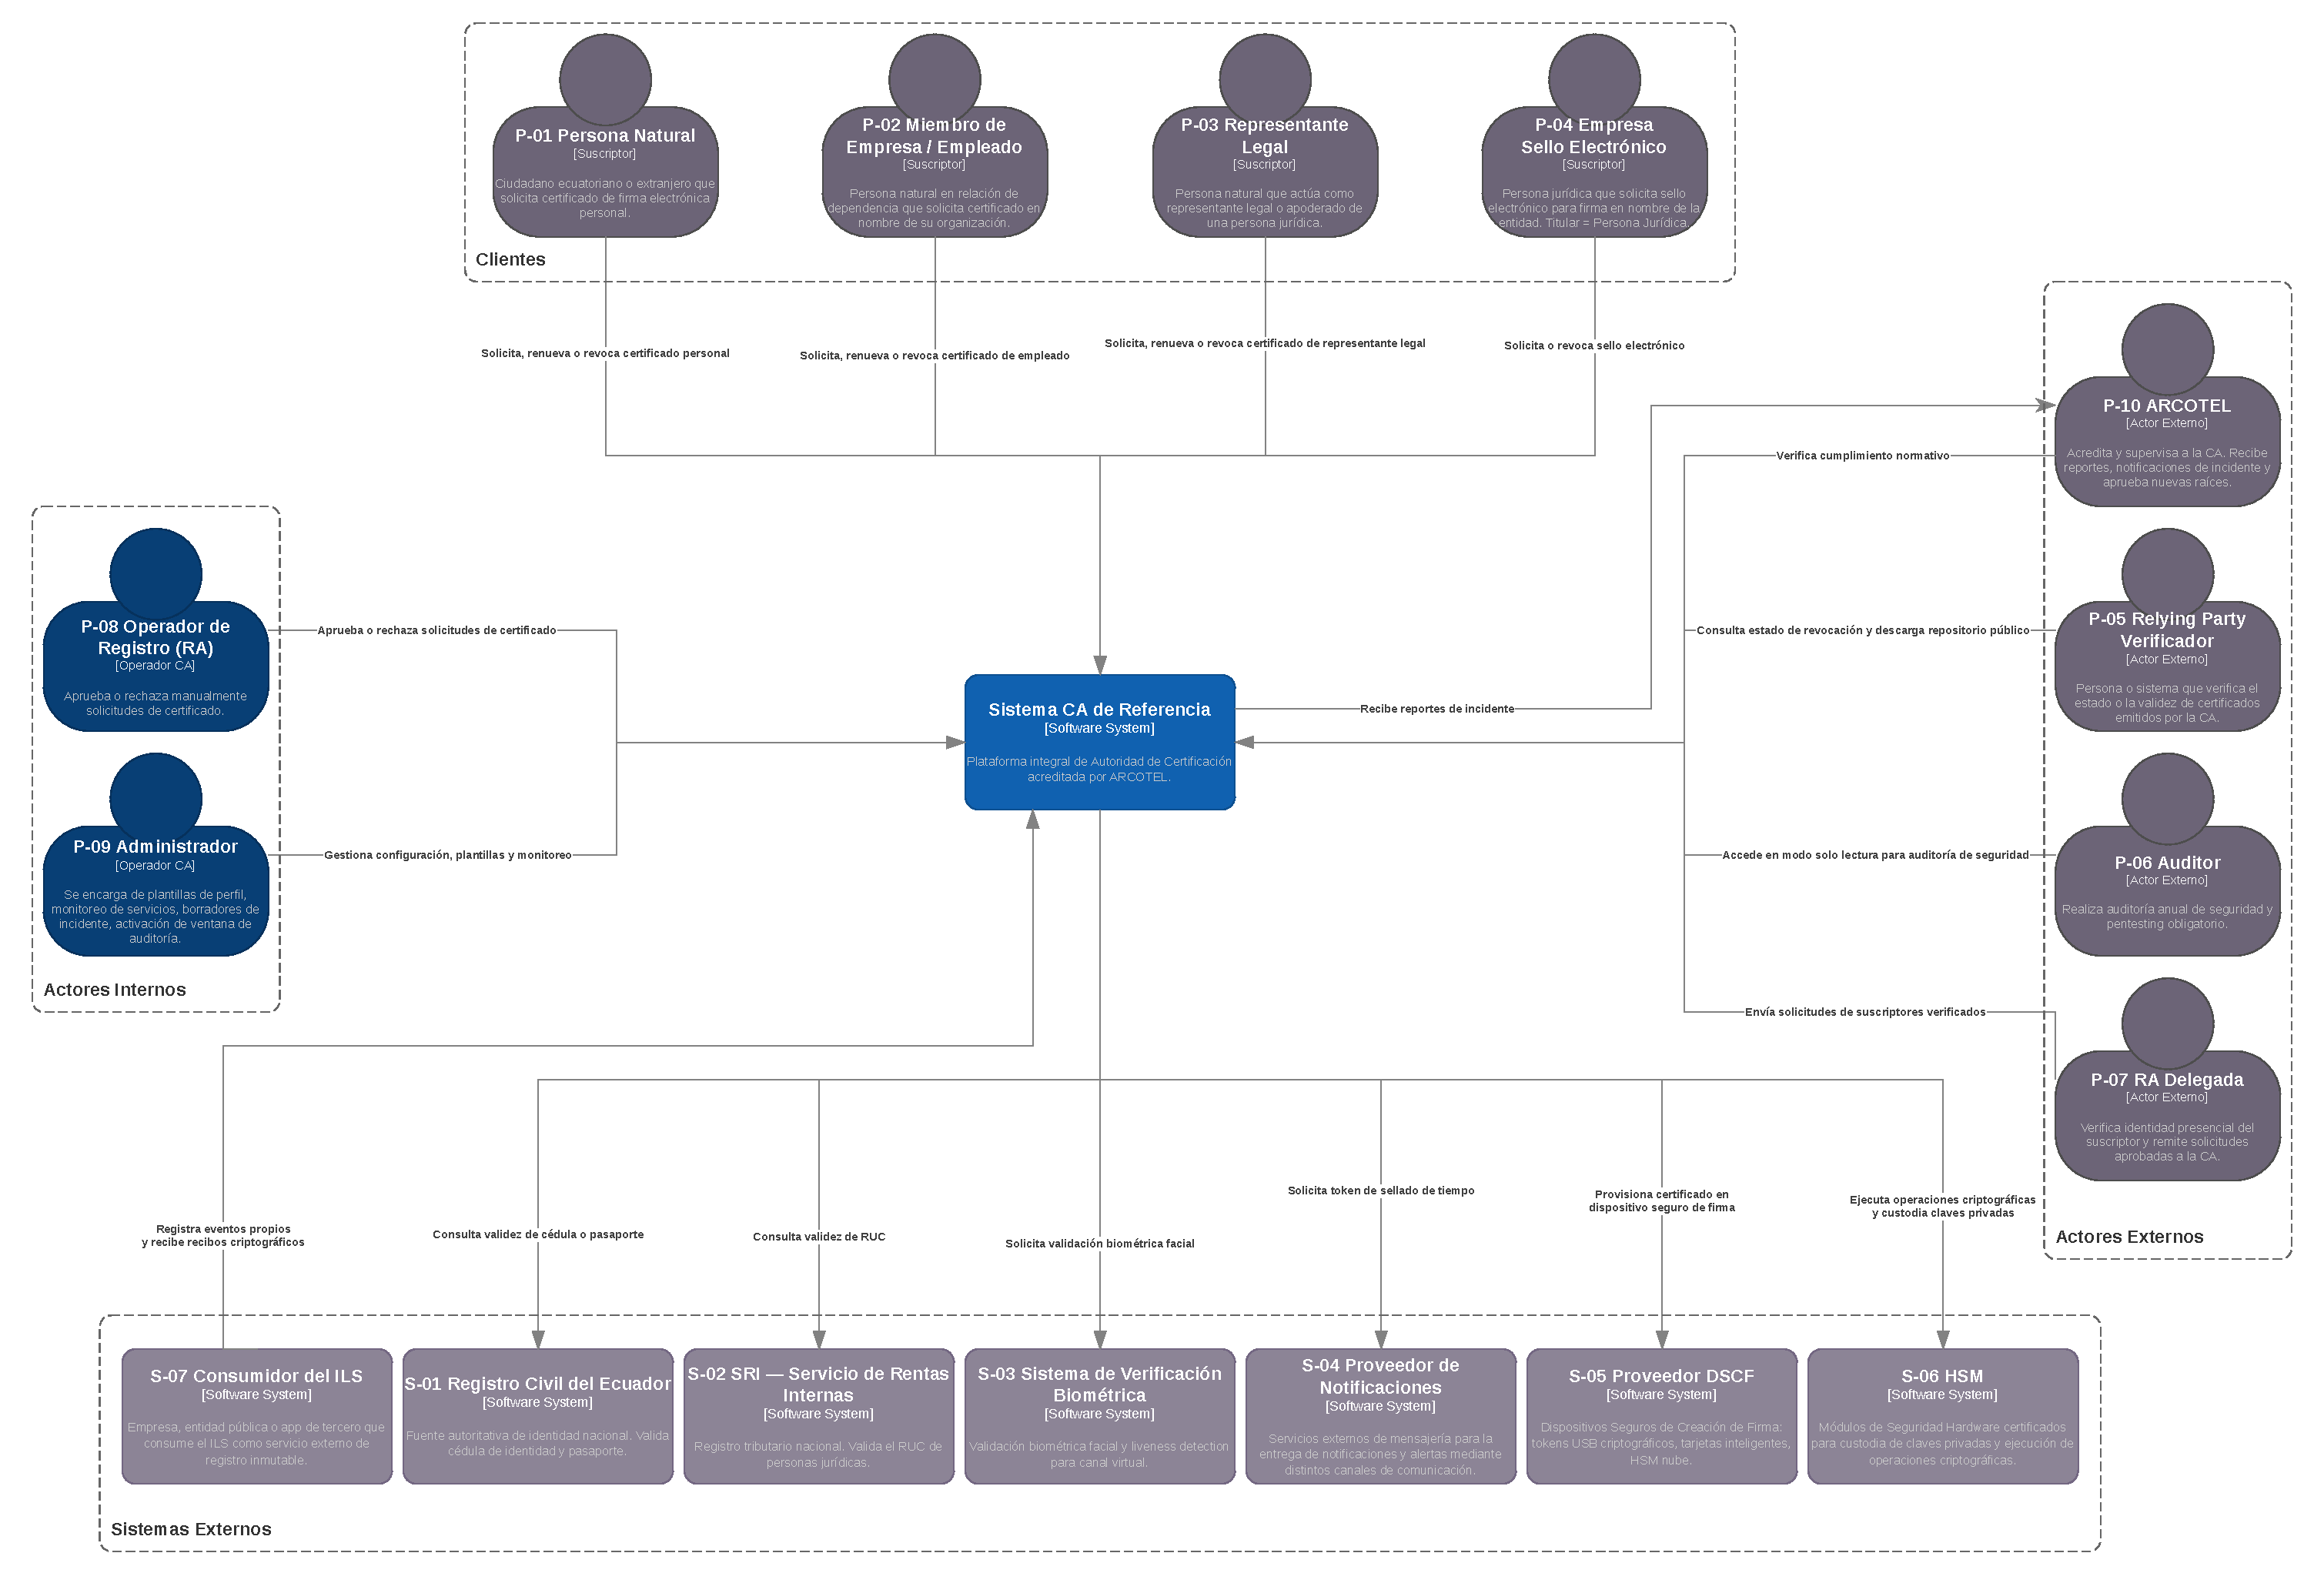
\includegraphics[width=\textwidth]{figs/resultados/c4-nv1.pdf}
\caption[Diagrama de Contexto C4 Nivel~1]{Diagrama de Contexto: el sistema CA de referencia
y sus actores externos.}
\label{fig:c4_n1}
\end{figure}

Como se observa, el sistema interactúa con cuatro categorías de actores externos. Los clientes (P-01 a
P-04) comprenden personas naturales, miembros de empresa, representantes legales y personas
jurídicas que solicitan, renuevan o piden una revocación de certificados conforme a los cuatro perfiles
regulados por ARCOTEL; su diversidad motiva el principio PA-07, puesto que cada perfil
tiene extensiones X.509 distintas sin que el motor de emisión requiera cambios. Los actores
externos comprenden a ARCOTEL (P-10), que acredita a la CA, recibe reportes, verifica
cumplimiento normativo y aprueba nuevas raíces, y al auditor externo de seguridad (P-06),
que accede en modo solo lectura para verificar la integridad del registro de auditoría sin
depender del operador. Los actores internos son el operador de registro (P-08),
que aprueba o rechaza solicitudes de certificado, y el administrador (P-09), que gestiona
configuración, plantillas de perfil y monitoreo. Los sistemas externos incluyen la
RA Delegada (P-07), que verifica identidad presencial y remite solicitudes ya aprobadas
vía interfaz mTLS, y el consumidor del ILS (S-07), entidad externa que registra sus propios
eventos en el log inmutable y recibe recibos criptográficos auditables.

JUnto a estos, seis sistemas externos adicionales completan el ecosistema: el Registro Civil (S-01) y el SRI (S-02)
validan cédula, pasaporte y RUC de personas jurídicas; el sistema de verificación biométrica
(S-03) ejecuta liveness detection para solicitudes por canal virtual; el proveedor de
notificaciones (S-04) distribuye alertas multicanal en nombre de la CA; el proveedor DSCF
(S-05) suministra dispositivos seguros de creación de firma (tokens USB, tarjetas
inteligentes y HSM en nube); y el HSM (S-06) custodia las claves privadas de la jerarquía
CA. Todos los sistemas externos se comunican con el sistema a través del contenedor
M-08 External Adapter Gateway, materializando el principio PA-02.

% ----------------------------------------------------------------------
\subsection{Análisis de Estilos Arquitectónicos y Decisión Adoptada}\label{subsec:estilos}

La selección del estilo base se apoyó en la evaluación comparativa de nueve estilos
arquitectónicos frente a diez criterios derivados de los Business Drivers y los Principios
Arquitectónicos establecidos en la Preliminary Phase de TOGAF. Los criterios
de peso alto cubren: bajo acoplamiento entre componentes, aislamiento de componentes
críticos, resiliencia ante fallos localizados, modificabilidad, trazabilidad y auditabilidad,
y consistencia transaccional de procesos críticos. Los criterios de peso medio cubren:
gobernabilidad operacional, independencia tecnológica, gestión eficiente de carga e
interoperabilidad con sistemas externos. Los nueve estilos evaluados siguen la clasificación
de Richards y Ford entre estilos monolíticos (Big Ball of Mud, Layered, Pipeline y
Microkernel) y distribuidos (Service-Based, Event-Driven, Space-Based, SOA con ESB y
Microservices) \cite{richards2020fundamentals}. La Figura~\ref{fig:estilos_chart} sintetiza el
resultado de la evaluación mostrando el número de criterios cumplidos y parcialmente
cumplidos por cada estilo.

\begin{figure}[H]
\centering
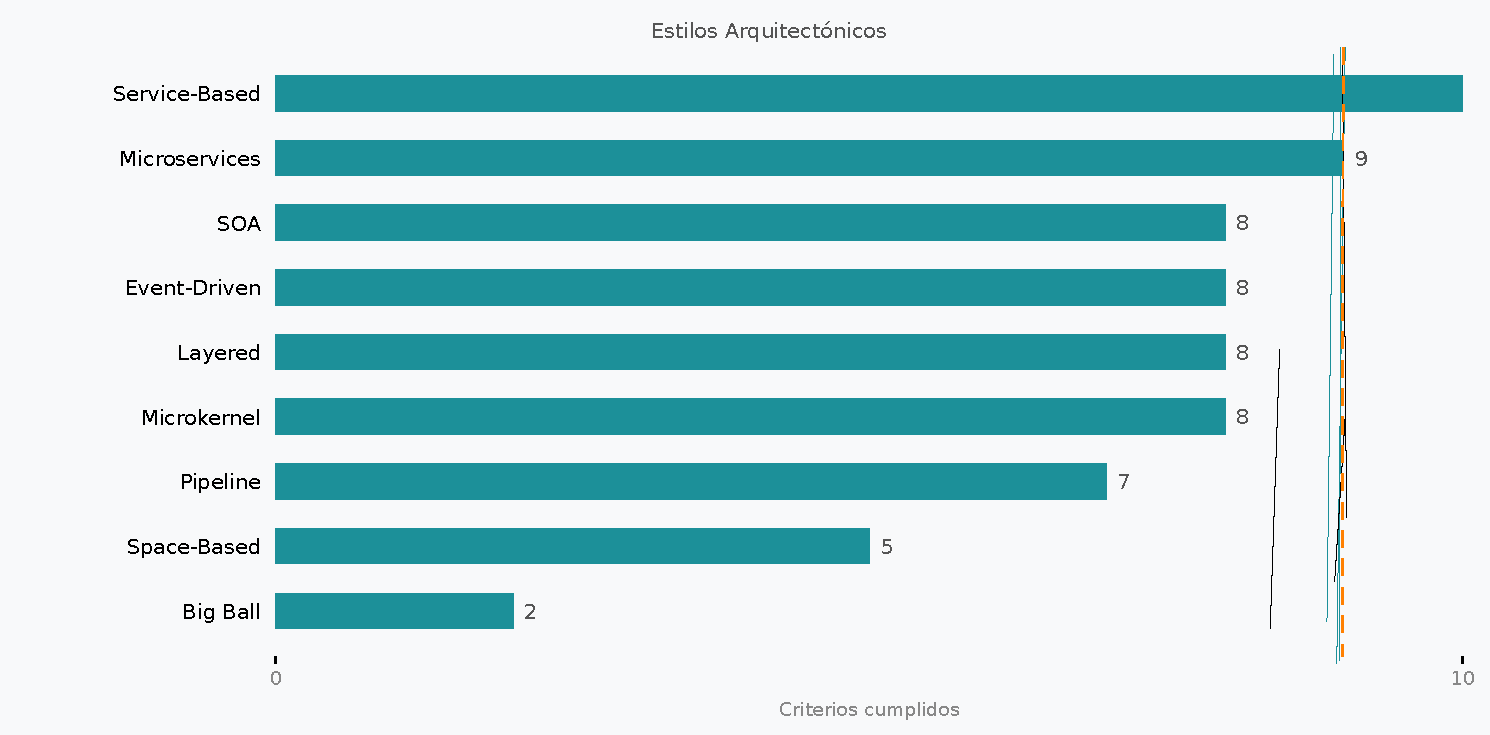
\includegraphics[width=\textwidth]{figs/resultados/arquitecturas_chart-1.pdf}
\caption[El estilo arquitectónico Service-Based es el que satisface la mayor cantidad de criterios de evaluación]
{El estilo arquitectónico Service-Based es el que satisface la mayor cantidad de criterios de evaluación.}
\label{fig:estilos_chart}
\end{figure}

El único estilo con cero evaluaciones negativas sobre los diez criterios es 
Service-Based Architecture, que obtiene resultado positivo en los seis criterios de peso
alto y en el criterio de interoperabilidad, presentando únicamente resultado parcial en el
criterio de gestión de carga, de peso medio. Los cuatro estilos monolíticos no satisfacen
la resiliencia ante fallos localizados porque comparten unidad de despliegue y un fallo en
cualquier componente compromete la totalidad del sistema. Event-Driven Architecture satisface siete criterios pero resulta inadecuada como base porque
la consistencia transaccional que los procesos de emisión y revocación exigen es incompatible
con la eventual consistency que la asincronía introduce: la normativa vigente exige que una
revocación se refleje de forma inmediata en las consultas OCSP, sin ventanas de consistencia
eventual \cite{arcotel20240176}. Microservices Architecture satisface igualmente siete
criterios, pero su operación exige infraestructura de orquestación de contenedores, mallas
de servicios y pipelines de CI/CD avanzados cuya complejidad es prohibitiva para las CA
ecuatorianas de tamaño medio; este factor de rechazo se documenta como ADR-06.

La deficiencia de Service-Based Architecture en el criterio de gestión de carga motiva una
composición dirigida por criterios: de Event-Driven Architecture se incorpora exclusivamente
la cola de mensajes persistente para flujos de menor criticidad: notificaciones, alertas y
registros no urgentes; la restricción explícita es que los flujos de emisión, revocación y
validación OCSP permanecen síncronos (ADR-07, ADR-08), de Microkernel Architecture se adopta
el patrón de extensión por configuración: un núcleo genérico de emisión que admite nuevos
perfiles normativos mediante plantillas sin modificar el código del motor, con lo que cada
nueva resolución ARCOTEL que introduzca un perfil de certificado se incorpora como
configuración, no como rediseño (ADR-06). La arquitectura resultante hereda los cero
resultados negativos de Service-Based Architecture y añade cobertura plena sobre el criterio
de gestión de carga mediante la cola asíncrona acotada a flujos no críticos.

% ----------------------------------------------------------------------
\subsection{Visión Arquitectónica}\label{subsec:vision_arq}

La Architecture Vision Statement sintetiza el resultado esperado de la arquitectura con
independencia de las decisiones de implementación.

\begin{quote}\itshape
Una Autoridad de Certificación acreditada en Ecuador que adopte esta arquitectura de
referencia opera sobre un motor de certificación modular y agnóstico al perfil: un conjunto
de servicios con responsabilidad única, comunicados exclusivamente mediante contratos de
interfaz explícitos y estándares abiertos, donde ningún cambio normativo de ARCOTEL requiere
rediseñar el motor de emisión, solo configurar una nueva plantilla. Los flujos operativos
secundarios se procesan de forma desacoplada sin comprometer la integridad ni la latencia de
las operaciones críticas. El resultado es reducción estructural del acoplamiento respecto a
sistemas PKI monolíticos, disponibilidad continua de validación, latencia de emisión
controlada, auditabilidad criptográficamente comprobable, cumplimiento normativo continuo con
ARCOTEL-2024-0176 y protección de datos personales por diseño conforme a la LOPDP.
\end{quote}

La Tabla~\ref{tab:restricciones_arq} resume las restricciones externas (regulatorias y de
seguridad) y las decisiones de diseño que las materializan estructuralmente.

\small
\begin{longtable}{@{}p{0.8cm}p{2.0cm}p{9.0cm}@{}}
\caption{Restricciones arquitectónicas y decisiones de diseño}\label{tab:restricciones_arq}\\
\toprule
\textbf{ID} & \textbf{Tipo} & \textbf{Descripción} \\
\midrule
\endfirsthead
\multicolumn{3}{l}{\small\itshape Continuación de la Tabla~\thetable}\\[2pt]
\toprule
\textbf{ID} & \textbf{Tipo} & \textbf{Descripción} \\
\midrule
\endhead
\bottomrule
\endlastfoot
RC-01 & Externa & RSA $\geq$\,2\,048\,bits usuarios finales, $\geq$\,4\,096\,bits infraestructura CA; SHA-256 mínimo (ARCOTEL Art.~13, 23) \\
\midrule
RC-02 & Externa & HSM FIPS~140-2 Level~3 y/o Common Criteria EAL4+ (ARCOTEL Art.~9) \\
\midrule
RC-03 & Externa & OCSP libre, gratuito, en tiempo real, sin autenticación de cliente (ARCOTEL Art.~4.17) \\
\midrule
RC-04 & Externa & Claves privadas CA nunca en claro fuera del HSM; la CA no accede a la clave privada del suscriptor (ARCOTEL Art.~4.6, 11b) \\
\midrule
RC-05 & Externa & Perfiles conformes a Anexos 1a--4b y 5--8 de ARCOTEL-2024-0176 más perfiles de extensibilidad \\
\midrule
RC-06 & Externa & Datos personales limitados a la necesidad del tratamiento; supresión al vencer la finalidad (LOPDP Art.~10(e)(i)) \\
\midrule
RC-07 & Externa & Publicación permanente e ininterrumpida de DPC, políticas, certificados emitidos, revocados y suspendidos (ARCOTEL Art.~4.7) \\
\midrule
D-01 & Diseño & El ILS registra hash criptográfico del payload; ningún dato personal en texto claro (PA-08) \\
\midrule
D-02 & Diseño & Toda comunicación inter-servicio se autentica con mTLS; certificados emitidos por la propia CA (PA-04) \\
\midrule
D-03 & Diseño & Cada servicio accede solo a su propio esquema de base de datos; ningún acceso cruzado a datos persistentes de otro (PA-02) \\
\midrule
D-04 & Diseño & El Message Broker Service es el canal principal de comunicación; async preferente; sync limitado a HSM, transacciones ACID, OCSP y queries con respuesta inmediata (ADR-31) \\
\end{longtable}
\normalsize

Estas decisiones clave explican por qué el diagrama de contenedores adopta su forma actual
y cómo cada contenedor se justifica por una decisión trazable. En conjunto, permiten
interpretar la arquitectura como una secuencia de elecciones estructurales coherentes y
alineadas con principios y restricciones previas.

% ----------------------------------------------------------------------
\subsection{Principios Arquitectónicos}\label{subsec:principios_arq}

Los ocho principios arquitectónicos gobiernan toda decisión técnica de la arquitectura de
referencia y establecen las restricciones que ninguna decisión puede violar. El catálogo
completo con justificaciones e implicaciones se presenta en la Tabla~\ref{tab:principios_inline}.

\small
\begin{longtable}{@{}p{0.75cm}p{3.0cm}p{8.0cm}@{}}
\caption{Principios arquitectónicos adoptados}\label{tab:principios_inline}\\
\toprule
\textbf{ID} & \textbf{Enunciado} & \textbf{Implicación principal} \\
\midrule
\endfirsthead
\multicolumn{3}{l}{\small\itshape Continuación de la Tabla~\thetable}\\[2pt]
\toprule
\textbf{ID} & \textbf{Enunciado} & \textbf{Implicación principal} \\
\midrule
\endhead
\bottomrule
\endlastfoot
PA-01 & Primacía de la norma & Algoritmos criptográficos, perfiles de certificado y mecanismos de validación están prescritos por LCE y ARCOTEL; no son elegibles libremente \\
\midrule
PA-02 & Separación de responsabilidades & Cada contenedor tiene una sola responsabilidad; ninguno accede directamente a los datos persistentes de otro; los contratos de interfaz son el único canal de comunicación \\
\midrule
PA-03 & Custodia criptográfica en hardware & Ninguna clave privada de la jerarquía CA existe en claro fuera de un HSM FIPS~140-2~L3; toda operación criptográfica se ejecuta dentro del perímetro del hardware \\
\midrule
PA-04 & Zero Trust & Toda comunicación inter-servicio se autentica con mTLS; los certificados de cliente son emitidos por la propia CA \\
\midrule
PA-05 & Trazabilidad e inmutabilidad & Toda operación del ciclo de vida genera una entrada en el ILS con encadenamiento criptográfico; el registro es comprobable offline sin acceso a la BD operativa \\
\midrule
PA-06 & Neutralidad tecnológica & La arquitectura prescribe estándares (PKCS\#11, RFC~6960, RFC~3161) e interfaces; el adoptante elige los productos que los implementen \\
\midrule
PA-07 & Extensibilidad sin rediseño & La incorporación de un nuevo perfil de certificado se limita a crear una plantilla en el catálogo; el motor de emisión no se modifica, no se recompila, no se redespliega \\
\midrule
PA-08 & Privacidad por diseño & El ILS registra el hash criptográfico del payload, no datos personales en claro; los datos del suscriptor residen exclusivamente en el esquema del servicio que los requiere; la privacidad por diseño implica además que los datos personales almacenados deben protegerse mediante cifrado en reposo \\
\end{longtable}
\normalsize

La tabla explicita la partición del sistema en unidades de despliegue con responsabilidades
claras y protocolos definidos, lo que facilita interpretar las fronteras de cambio y de
datos. En conjunto, se observa el equilibrio entre flujos síncronos críticos y canales
asíncronos, preservando aislamiento y trazabilidad sin comprometer la operación normativa.

% ----------------------------------------------------------------------
\subsection{Decisiones Arquitectónicas Clave}\label{subsec:adrs_principales}

Las decisiones arquitectónicas clave se formalizan como ADRs siguiendo la metodología TOGAF
ADM (ADR-02). La Tabla~\ref{tab:adrs_core} recoge los diez ADRs que directamente condicionan
la estructura del diagrama de contenedores (C4~N2); el catálogo completo de 39 ADRs se
documenta en el \hyperref[anx:adrs]{Anexo~G}.

\footnotesize
\begin{longtable}{@{}p{0.9cm}p{4.5cm}p{3.0cm}p{3.4cm}@{}}
\caption{ADRs con impacto directo en el diseño de contenedores (C4~N2)}\label{tab:adrs_core}\\
\toprule
\textbf{ADR} & \textbf{Decisión} & \textbf{Consecuencia} & \textbf{ADRs relacionados} \\
\midrule
\endfirsthead
\multicolumn{4}{l}{\footnotesize\itshape Continuación de la Tabla~\thetable}\\[2pt]
\toprule
\textbf{ADR} & \textbf{Decisión} & \textbf{Consecuencia} & \textbf{ADRs relacionados} \\
\midrule
\endhead
\bottomrule
\endlastfoot
ADR-04 & HSM FIPS~140-2~L3 obligatorio para claves CA y par del suscriptor generado por la CA &
  Crea el contenedor M-04 HSM Integration Service como única interfaz PKCS\#11 al hardware &
  PA-03 · RC-02 \\
\midrule
ADR-06 & Adoptar estilo compuesto EA-10 (Service-Based + elementos de Event-Driven y Microkernel) &
  10 contenedores de grano grueso con BD compartida DS-01; arquitectura sin microservicios &
  ADR-07 · ADR-08 · ADR-31 \\
\midrule
ADR-07 & RA Service (BFF) y RA Portal (SPA) como unidades de despliegue separadas &
  Crea M-06 RA Service y M-09 RA Portal como contenedores independientes; RBAC centralizado en M-06 &
  ARCOTEL-2024-0176 \\
\midrule
ADR-08 & Microkernel en catálogo de perfiles: núcleo genérico más plantillas intercambiables por perfil &
  Nuevo perfil ARCOTEL = nueva plantilla de configuración; sin modificar M-01 CA Core Service &
  PA-07 · RC-05 \\
\midrule
ADR-09 & Modelo de aislamiento HSM de 6 capas (Monitor Object + Scoped Locking + Lifecycle Callback) &
  M-04 implementa zeroize FIPS~140-2 al destruir sesiones PKCS\#11; protección ante excepciones no manejadas &
  ADR-13 · ADR-22 \\
\midrule
ADR-23 & External Adapter Gateway como Anti-Corruption Layer (ACL) stateless con Plugin Registry &
  Crea M-08 External Adapter Gateway; M-06 no invoca APIs externas directamente (Ce RA Service $\leq$\,5) &
  ADR-25 · PA-02 \\
\midrule
ADR-27 & Message Broker Service con interfaz abstracta \texttt{IMessageBroker} como canal principal &
  Crea M-10 Message Broker Service; productores publican vía \texttt{IMessageBroker.publish()} post-commit &
  ADR-31 · ADR-32 · ADR-35 \\
\midrule
ADR-31 & Comunicación asíncrona preferente; sync limitado a HSM, ACID, OCSP, queries con respuesta inmediata &
  Supersede restricciones previas sobre sync; interacciones nuevas asumen async por defecto &
  ADR-27 · D-04 \\
\midrule
ADR-33 & Ce (Acoplamiento Eferente) $\leq$\,5 como métrica de diseño a nivel C4~N2 &
  Ningún contenedor referencia más de 5 contenedores externos; Ce mide acoplamiento saliente &
  NFR-19 · PA-02 \\
\midrule
ADR-39 & TTL caché OCSP = 5s con invalidación activa síncrona por CRL Service (Observer síncrono) &
  Ventana máxima de inconsistencia 5s; invalidación activa reduce a $<$\,1s nominal en revocación &
  RC-03 · NFR-06 \\
\end{longtable}
\normalsize

Los diez ADRs expuestos operan como restricciones de diseño: cada contenedor del diagrama
C4~N2 existe porque al menos un ADR lo crea o delimita su alcance, y ningún contenedor
puede modificar su protocolo de comunicación sin revisar el ADR correspondiente. La
trazabilidad completa entre decisiones, consecuencias y métricas de acoplamiento garantiza
que la arquitectura sea auditable en su proceso de construcción, no solo en su resultado.

% ----------------------------------------------------------------------
\subsection{Nivel 2 --- Diagrama de Contenedores}\label{subsec:c4_n2}

Con la visión arquitectónica, los principios y los ADRs establecidos, el diagrama de
contenedores materializa esas decisiones en unidades de despliegue concretas. La
Figura~\ref{fig:c4_n2} presenta el diagrama completo.

\begin{figure}[H]
\centering
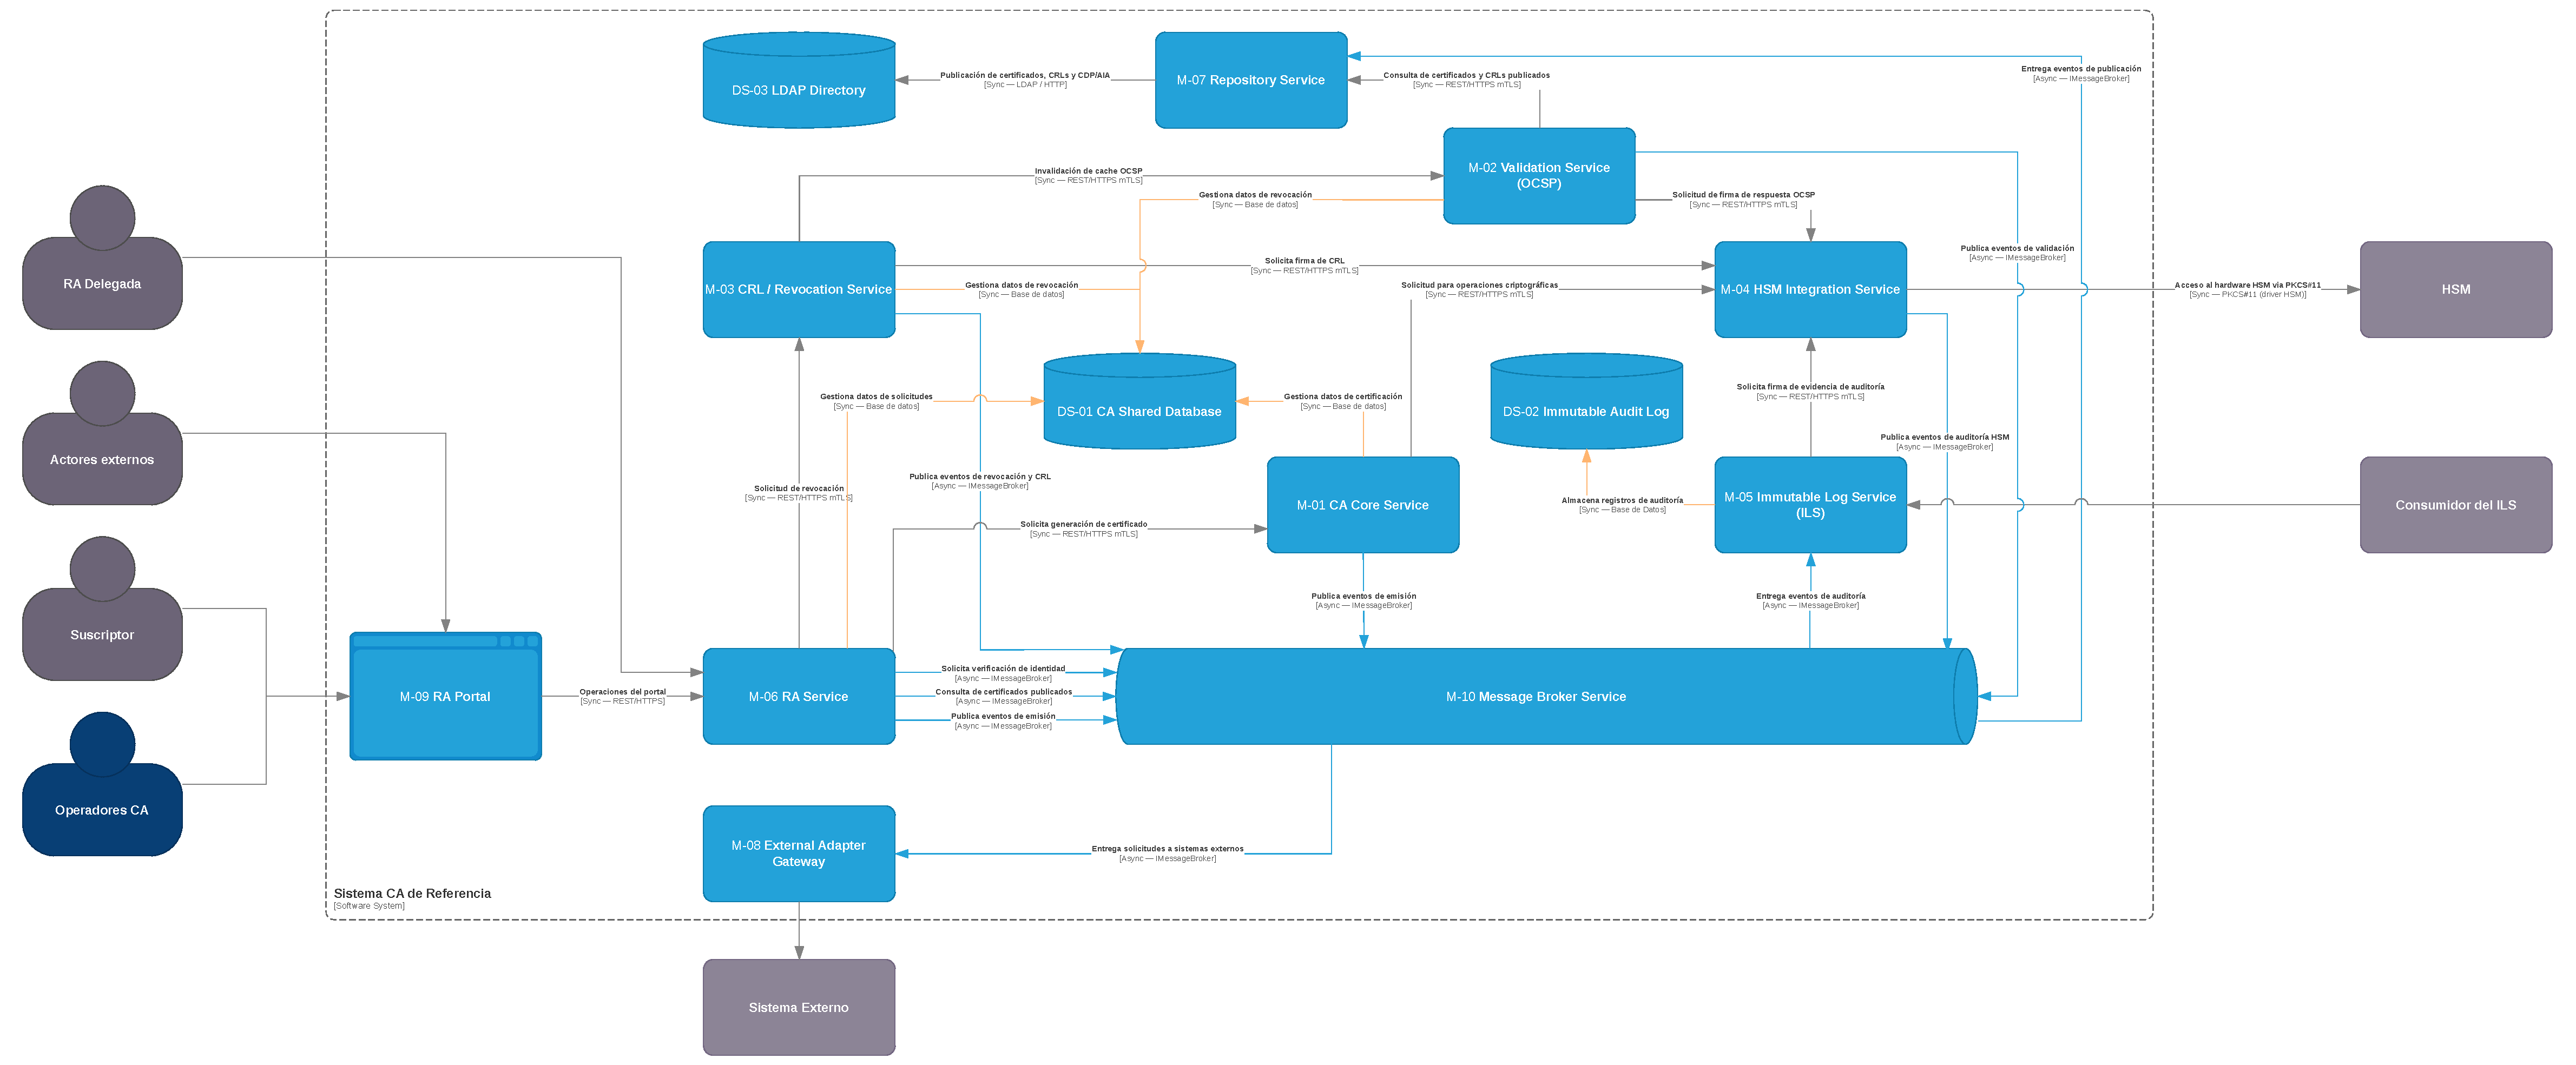
\includegraphics[width=\textwidth]{figs/resultados/c4-nv2.pdf}
\caption[Diagrama de Contenedores C4 Nivel~2]{Diagrama de Contenedores de la arquitectura
de referencia.}
\label{fig:c4_n2}
\end{figure}

El diagrama expone diez contenedores de grano grueso organizados alrededor de una base de
datos compartida (DS-01) con esquemas aislados por contenedor. El canal de comunicación
principal es asíncrono vía \texttt{IMessageBroker} (ADR-27); las interacciones síncronas
quedan acotadas a las operaciones con el HSM, las transacciones ACID de revocación, el
protocolo OCSP y las consultas con respuesta inmediata. El estilo compuesto EA-10 es
visible en la coexistencia de contenedores de servicio grueso (M-01 a M-09) con un
contenedor de mensajería desacoplada (M-10 Message Broker Service) y un núcleo de catálogo
extensible por configuración (ADR-08). La Tabla~\ref{tab:contenedores} detalla la
responsabilidad y protocolo principal de cada contenedor.

\footnotesize
\begin{longtable}{@{}p{2.3cm}p{1.4cm}p{5.5cm}p{2.5cm}@{}}
\caption{Contenedores de la arquitectura de referencia}\label{tab:contenedores}\\
\toprule
\textbf{Contenedor} & \textbf{Tipo} & \textbf{Responsabilidad} & \textbf{Protocolo principal} \\
\midrule
\endfirsthead
\multicolumn{4}{l}{\footnotesize\itshape Continuación de la Tabla~\thetable}\\[2pt]
\toprule
\textbf{Contenedor} & \textbf{Tipo} & \textbf{Responsabilidad} & \textbf{Protocolo principal} \\
\midrule
\endhead
\bottomrule
\endlastfoot
M-01 CA Core Service & App &
  Gestiona la emisión de certificados X.509 y coordina la generación de claves y la firma
  digital con el HSM &
  REST/HTTPS mTLS · Síncr.\newline \texttt{IMessageBroker} · Asíncr. \\
\midrule
M-02 Validation Service (OCSP) & App &
  Responde consultas de estado de certificados conforme RFC~6960; caché pre-firmada para
  SLA bajo carga (TTL 5s, invalidación activa) &
  REST/HTTPS · Síncr. (OCSP queries)\newline \texttt{IMessageBroker} · Asíncr. \\
\midrule
M-03 CRL / Revocation Service & App &
  Administra la revocación y suspensión de certificados; publica CRLs ordinarias y
  extraordinarias; notifica a OCSP síncronamente al revocar &
  REST/HTTPS mTLS · Síncr.\newline \texttt{IMessageBroker} · Asíncr. \\
\midrule
M-04 HSM Integration Service & App &
  Abstrae y coordina el acceso al HSM para ejecución de operaciones criptográficas;
  FIPS~140-2~L3; quórum 3-of-5 para claves CA &
  PKCS\#11 v2.40 (driver HSM)\newline REST/HTTPS mTLS · Síncr. \\
\midrule
M-05 Immutable Log Service (ILS) & App &
  Registra evidencias auditables con encadenamiento criptográfico; confirmación selectiva
  de eventos de alta relevancia regulatoria en Hyperledger Fabric 2.5 &
  REST/HTTPS mTLS · Síncr. (firma HSM)\newline \texttt{IMessageBroker} · Asíncr. (consume eventos) \\
\midrule
M-06 RA Service (BFF) & App &
  Gestiona la validación de identidad y la aprobación de solicitudes de certificado;
  Backend for Frontend con RBAC conforme ARCOTEL-2024-0176 &
  REST/HTTPS mTLS · Síncr.\newline \texttt{IMessageBroker} · Asíncr. \\
\midrule
M-07 Repository Service & App &
  Publica certificados, CRLs, cadenas de confianza y documentos de política de la CA;
  endpoint de consulta pública por número de serie (ARCOTEL Art.~4.7) &
  LDAP / HTTP · Síncr. (CDP/AIA)\newline \texttt{IMessageBroker} · Asíncr. (consume eventos) \\
\midrule
M-08 External Adapter Gateway & Infra. &
  Anti-Corruption Layer (ACL) stateless con Plugin Registry para sistemas externos
  (Registro Civil S-01, SRI S-02, biométrico S-03, TSA S-04); Ce~=~1 &
  REST/HTTPS · Síncr. (adaptadores)\newline \texttt{IMessageBroker} · Asíncr. (consume eventos) \\
\midrule
M-09 RA Portal & Web &
  SPA (Single Page Application) para operadores y suscriptores; stateless, sin BD propia;
  interactúa exclusivamente con M-06 &
  REST/HTTPS · Síncr.\newline WebSocket (notificaciones tiempo real) \\
\midrule
M-10 Message Broker Service & Infra. &
  Canal principal de comunicación asíncrona entre contenedores mediante publicación y
  suscripción de eventos; interfaz abstracta \texttt{IMessageBroker} (ADR-27, ADR-32) &
  \texttt{IMessageBroker} · Asíncr. \\
\midrule
DS-01 CA Shared Database & BD &
  Almacena los datos operacionales de los servicios de certificación; esquemas aislados por
  servicio (Data Mapper ADR-30); sin acceso cruzado entre contenedores &
  Base de datos · Schemas aislados \\
\midrule
DS-02 Immutable Audit Log & BD &
  Almacena las evidencias inmutables de auditoría con encadenamiento criptográfico y firma
  HSM; modo append-only; implementación: Hyperledger Fabric 2.5 &
  Base de datos · Append-only \\
\midrule
DS-03 LDAP Directory & Directorio &
  Almacena y publica certificados, CRLs y cadenas de confianza conforme RFC~5280 (CDP/AIA);
  acceso público de lectura &
  LDAP \\
\end{longtable}
\normalsize

La arquitectura materializa el principio PA-02 mediante la asignación de un único esquema de
datos por contenedor: ningún servicio accede directamente a los datos persistentes de otro
(ADR-30). La comunicación asíncrona entre contenedores se realiza mediante publicación
directa post-commit a través de la interfaz \texttt{IMessageBroker} (ADR-27, ADR-32);
los productores dependen únicamente del contrato abstracto, sin conocer a sus suscriptores.
El broker opera como capa de transporte no confiable por diseño: la integridad de los
mensajes queda garantizada por la firma del \textit{Command} (ADR-10) y el token de un
solo uso (ADR-28), que permiten al \textit{CommandProcessor} rechazar cualquier mensaje
manipulado o reinyectado sin ejecutar ninguna operación de dominio. 
El HSM permanece fuera del perímetro del sistema
como sistema externo, accedido exclusivamente por M-04 mediante PKCS\#11~v2.40,
materializando el principio PA-03. La métrica de acoplamiento eferente Ce se mantiene en
promedio de 2,7 arcos por contenedor; la única excepción es M-06 con Ce~=~6, valor que
supera el umbral Ce~$\leq$~5 de ADR-33 y está documentado como consecuencia aceptada de su
rol de orquestador BFF del portal RA.

% ----------------------------------------------------------------------
\subsection{Nivel 3 --- Diagramas de Componentes}\label{subsec:c4_n3}

Los diagramas de componentes (C4 Nivel~3) detallan la estructura interna de cada contenedor
arquitectónicamente relevante, describiendo cómo se organiza la lógica interna y cómo se
materializan los patrones tácticos establecidos en los ADRs de la Sección~\ref{subsec:adrs_principales}
y documentados en el \hyperref[anx:tacticos_artefacts]{Anexo~F}.
Se examinan los cuatro contenedores con mayor relevancia estructural: M-01 CA Core Service,
M-02 Validation Service (OCSP), M-03 CRL / Revocation Service y M-05 Immutable Log Service.

% --- M-01 -----------------------------------------------------------
El primer contenedor, M-01 CA Core Service, concentra la lógica de emisión de certificados X.509.
La Figura~\ref{fig:c4_n3_m01} expone sus once componentes internos organizados en tres
capas: la entrada REST/mTLS (\texttt{CertificateIssuanceController}), la orquestación
transaccional (\texttt{IssuanceOrchestrator}, \texttt{IssuancePipeline} y
\texttt{SubjectDataFormatValidator}) y la capa de persistencia y publicación
(\texttt{CertificateRepository}, \texttt{EventPublisher} y \texttt{CertificatePublisher}).

\begin{figure}[H]
\centering
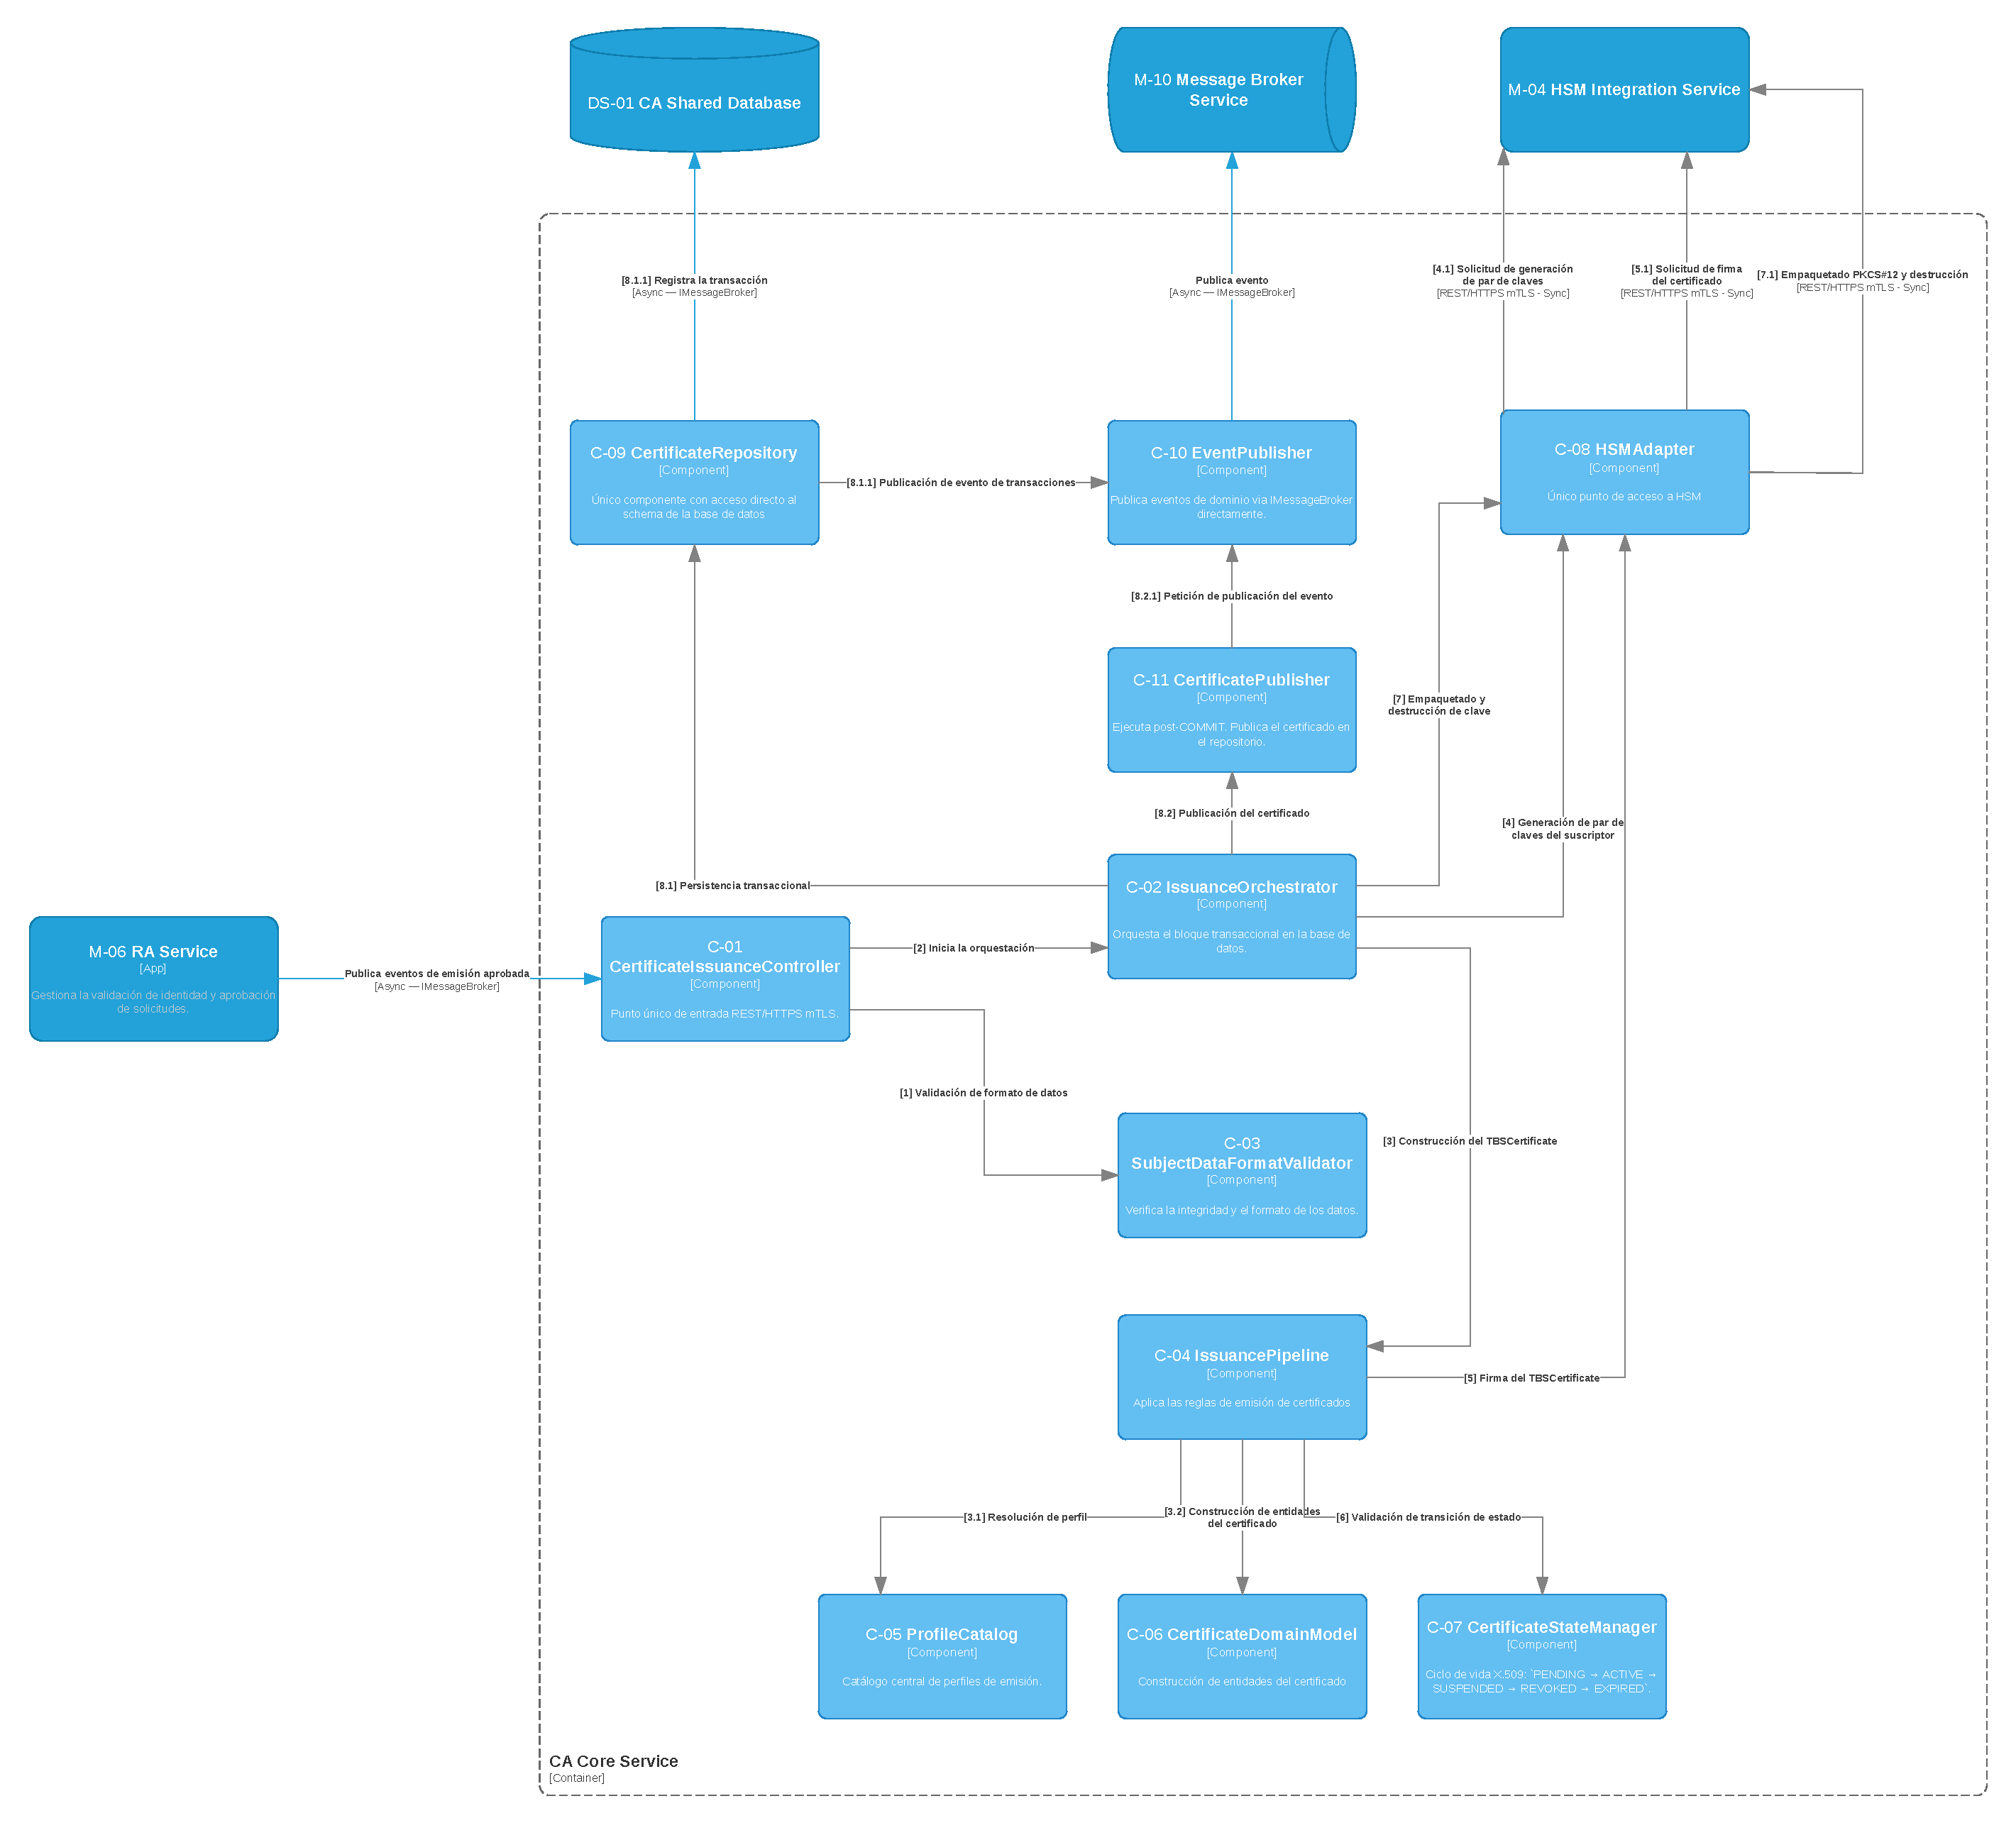
\includegraphics[width=\textwidth]{figs/resultados/m01-c4-nv3.pdf}
\caption[C4 N3: M-01 CA Core Service]{Diagrama de componentes del contenedor M-01 CA Core Service.}
\label{fig:c4_n3_m01}
\end{figure}

El diseño revela varios invariantes tácticos. La restricción de acoplamiento Ce~$\leq$~5
(ADR-33) se mantiene al concentrar todo el acceso a la base de datos en el único
\texttt{CertificateRepository} y el acceso al HSM en \texttt{HSMAdapter}. El
\texttt{ProfileCatalog} actúa como punto de extensión del núcleo Microkernel (ADR-08):
nuevos perfiles de emisión se incorporan sin modificar la lógica del \texttt{IssuancePipeline}.
El \texttt{CertificateStateManager} formaliza la máquina de estados X.509
(\texttt{PENDING $\rightarrow$ ACTIVE $\rightarrow$ SUSPENDED $\rightarrow$ REVOKED
$\rightarrow$ EXPIRED}) como componente independiente, separando el ciclo de vida del acto
de emisión. El \texttt{EventPublisher} publica eventos directamente post-commit vía
\texttt{IMessageBroker} (ADR-27), en coherencia con la latencia de emisión exigida por NFR-05. 

% --- M-02 -----------------------------------------------------------
El contenedor M-02 complementa a M-01 desde
la perspectiva de los clientes verificadores: mientras M-01 emite, M-02 responde a las
consultas de estado de los certificados activos. La Figura~\ref{fig:c4_n3_m02} detalla 
los nueve componentes del contenedor M-02 Validation
Service (OCSP), responsable de responder a consultas de estado de certificados en tiempo
real conforme al protocolo RFC~6960. El diagrama permite observar cómo el diseño resuelve
simultáneamente dos requisitos en tensión: alta disponibilidad de respuesta y coherencia
inmediata tras una revocación.

\begin{figure}[H]
\centering
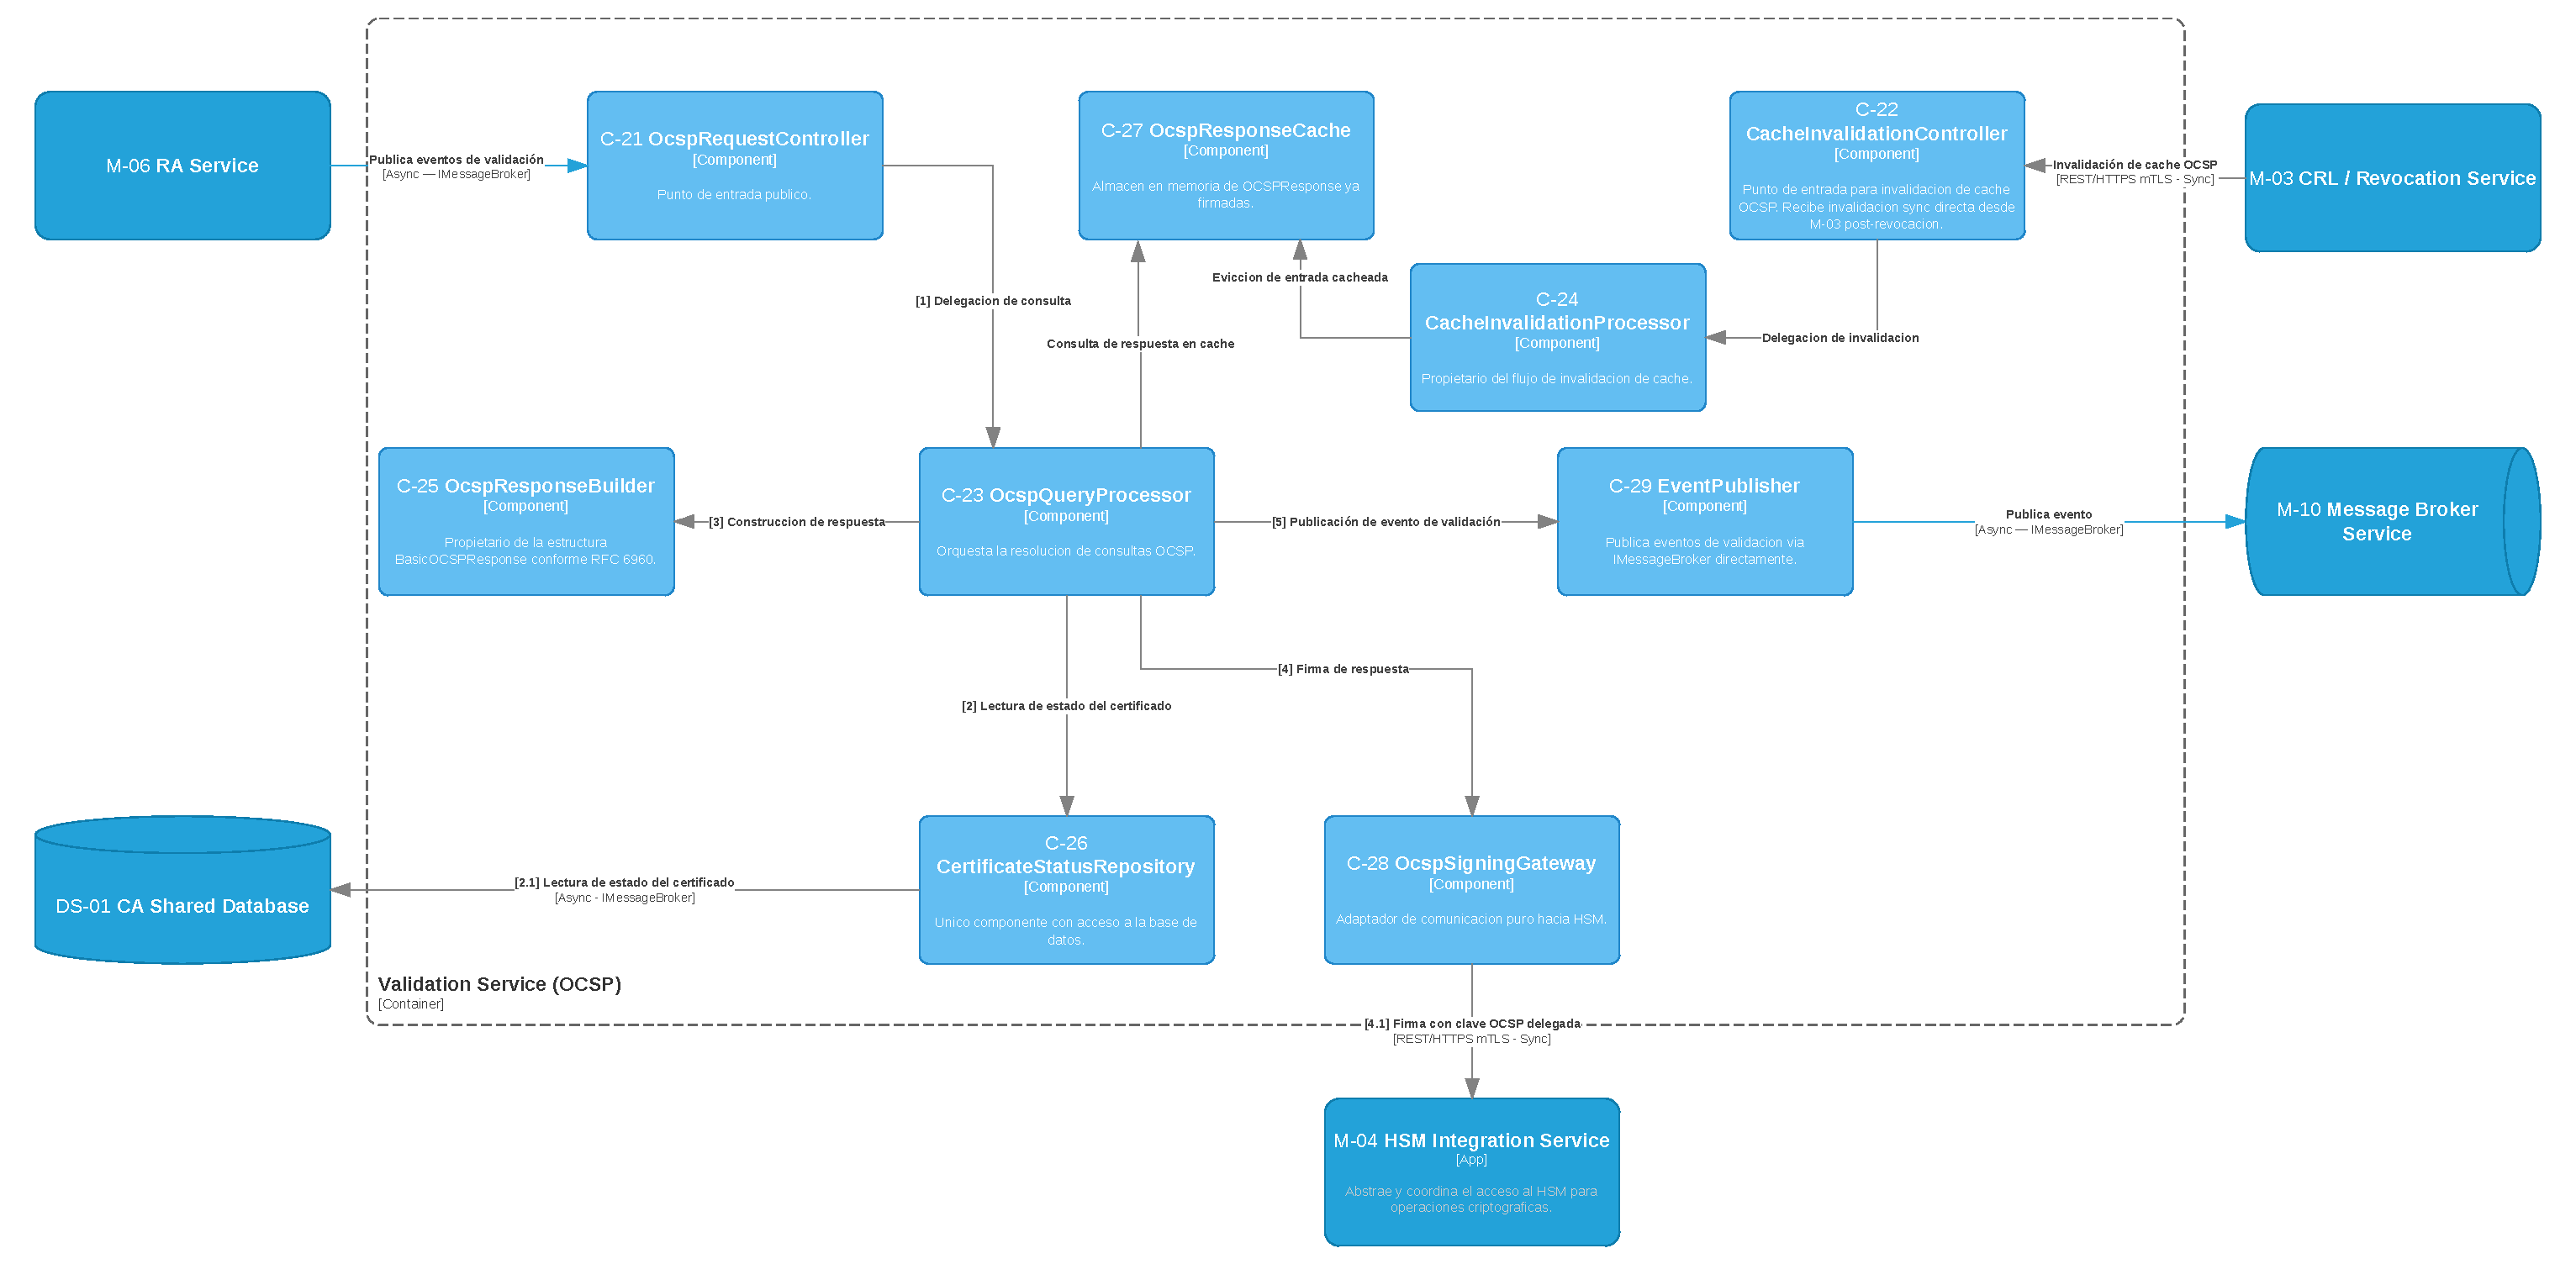
\includegraphics[width=\textwidth]{figs/resultados/m02-c4-nv3.pdf}
\caption[C4 N3: M-02 Validation Service (OCSP)]{Diagrama de componentes del contenedor M-02 Validation Service (OCSP).}
\label{fig:c4_n3_m02}
\end{figure}

El componente más crítico en términos de rendimiento es \texttt{OcspResponseCache}, que
almacena en memoria las respuestas OCSP ya firmadas y reduce las invocaciones al HSM a
solo las entradas sin caché. La gestión de invalidación es explícita y síncrona:
\texttt{CacheInvalidationController} recibe notificación directa de M-03 post-revocación,
y \texttt{CacheInvalidationProcessor} elimina la entrada del certificado revocado sin
consultar la base de datos, minimizando el acoplamiento eferente de ese flujo.
\texttt{OcspResponseBuilder} es el único propietario de la estructura
\texttt{BasicOCSPResponse}, manteniendo la conformidad con RFC~6960 en un único punto.
El \texttt{OcspSigningGateway} actúa como adaptador puro hacia M-04 (HSM Integration
Service), garantizando que las respuestas OCSP se firmen con la clave delegada del OCSP
Responder y nunca con la clave raíz de la CA. 

% --- M-03 -----------------------------------------------------------
La siguiente figura examina M-03, el
contenedor que origina las notificaciones de revocación que M-02 consume. 
La Figura~\ref{fig:c4_n3_m03} presenta los diez componentes de M-03 CRL / Revocation
Service. Este contenedor tiene responsabilidad dual: procesar comandos de revocación
individuales y generar periódicamente las listas de certificados revocados (CRL) conformes
al estándar RFC~5280. El diagrama expone cómo ambos flujos comparten la misma base de datos
pero operan con lógicas de control independientes.

\begin{figure}[H]
\centering
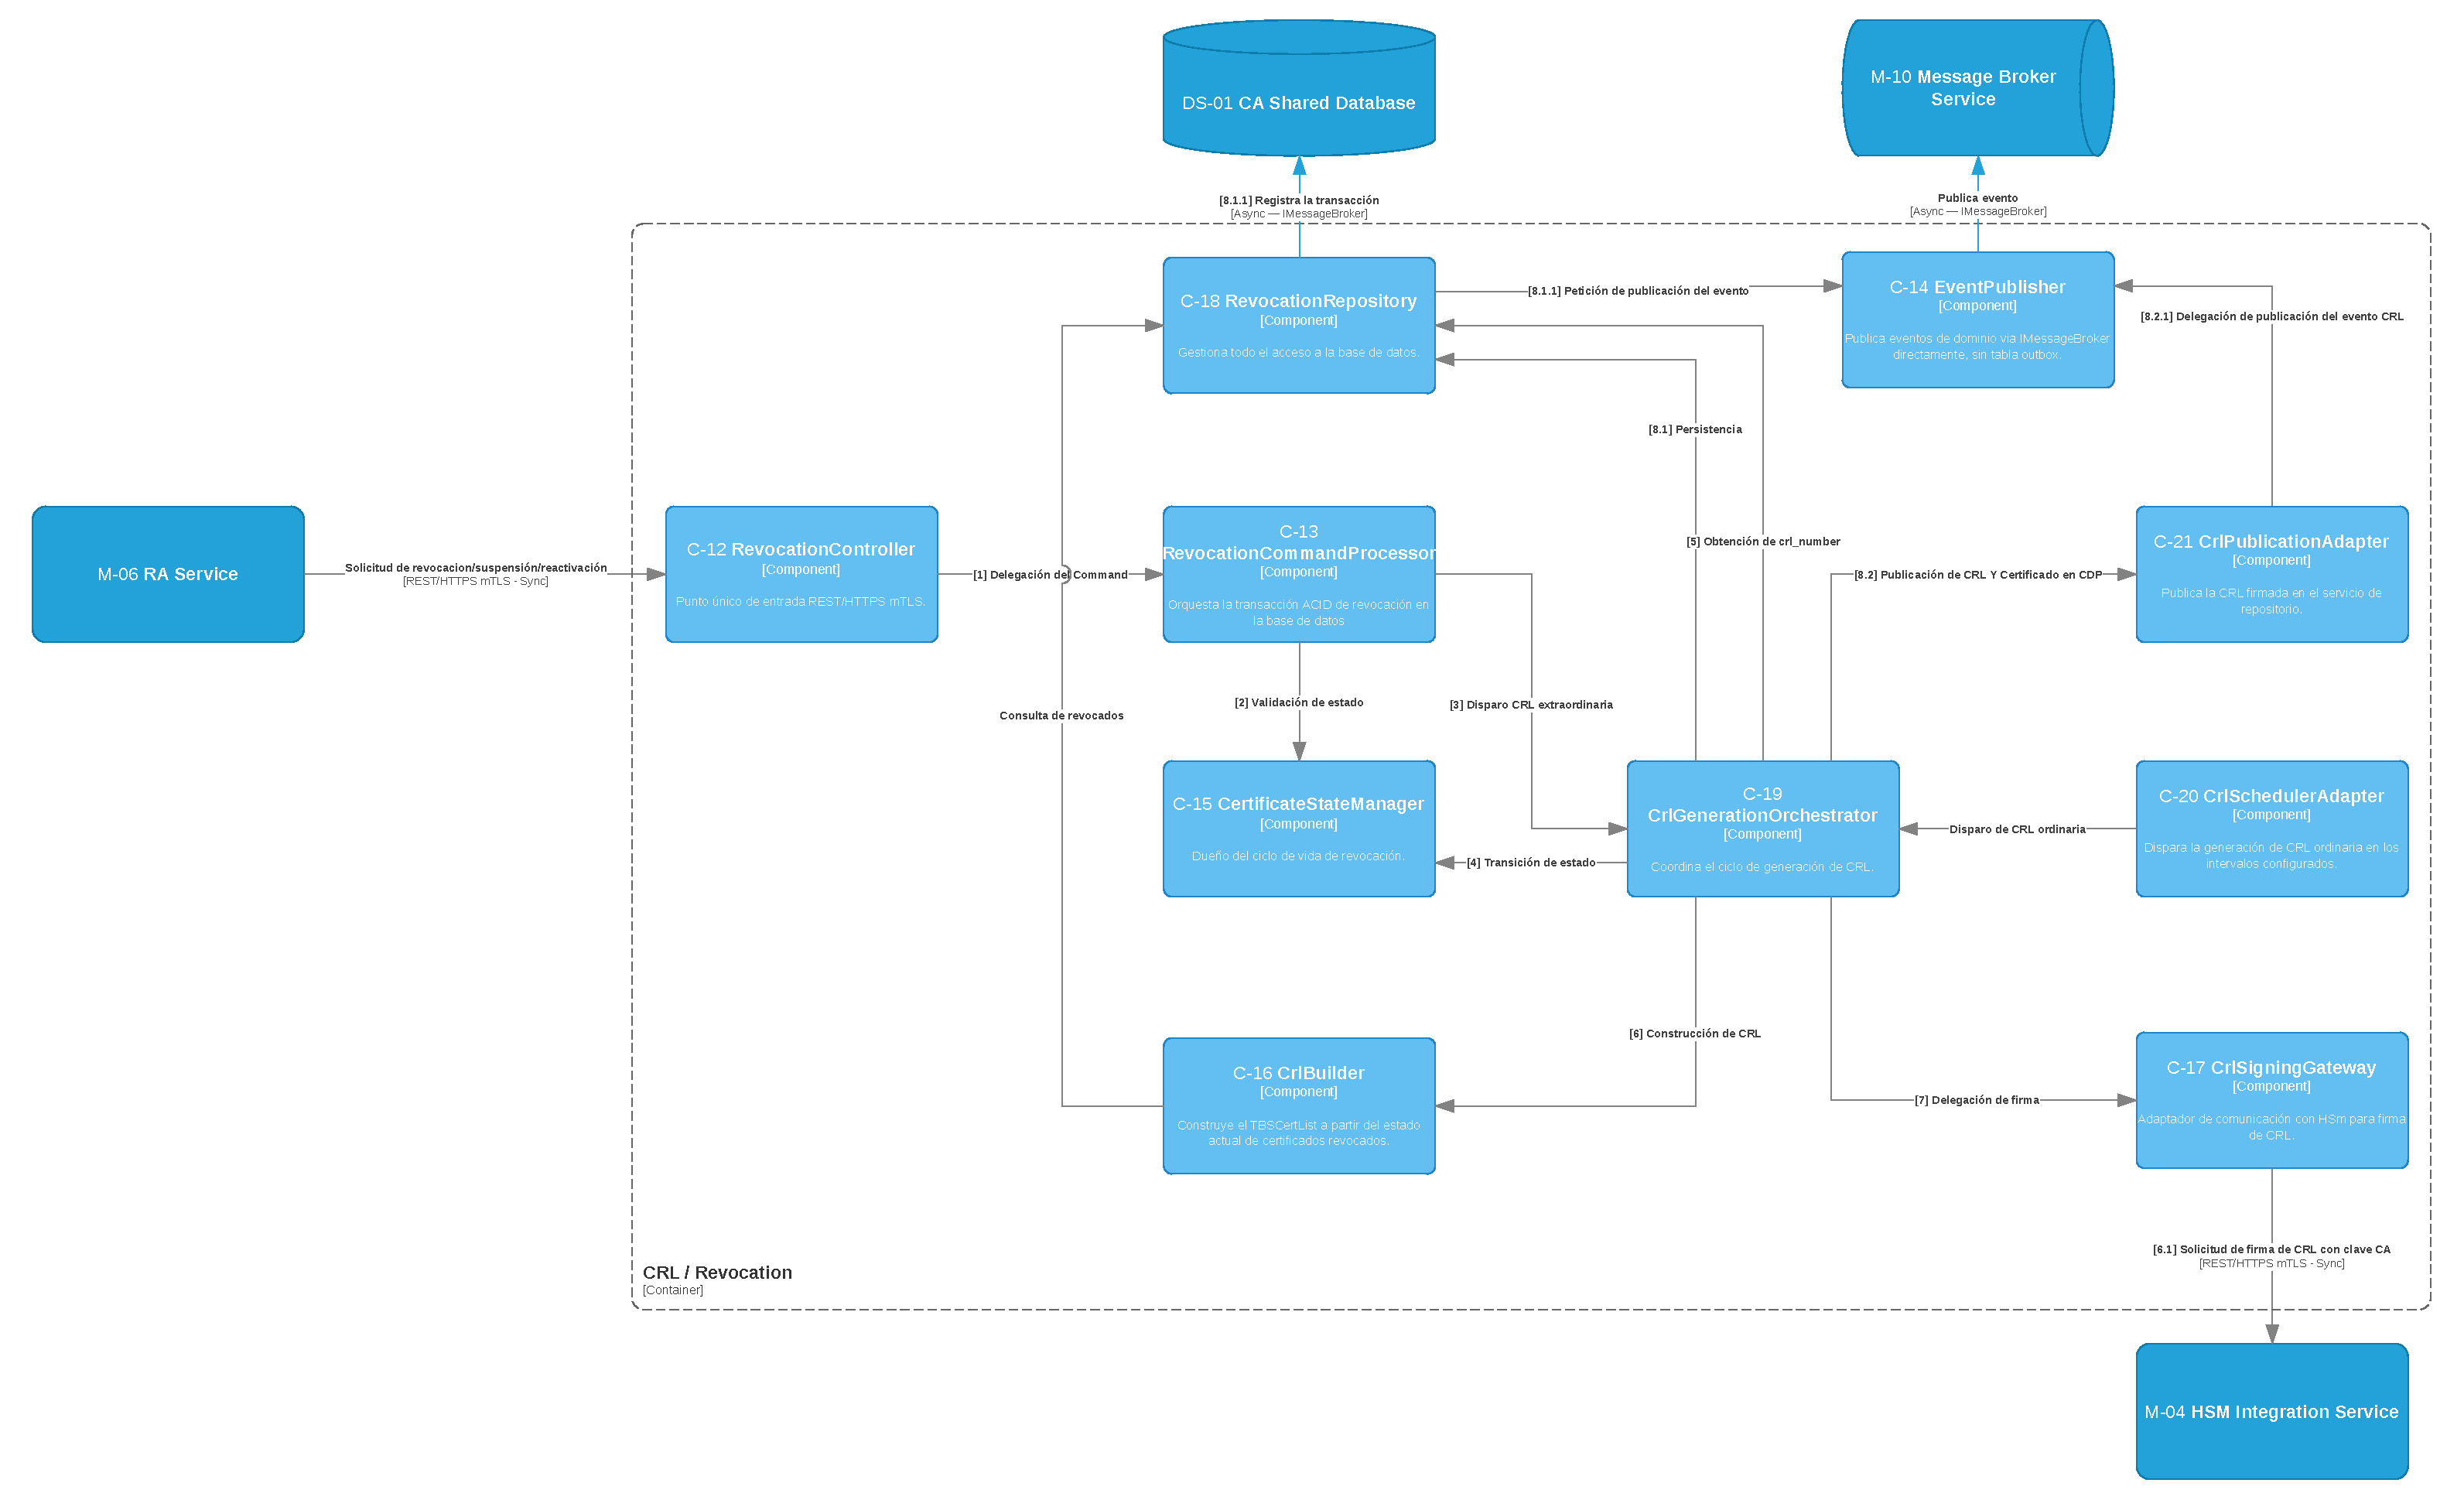
\includegraphics[width=\textwidth]{figs/resultados/m03-c4-nv3.pdf}
\caption[C4 N3: M-03 CRL / Revocation Service]{Diagrama de componentes del contenedor M-03 CRL / Revocation Service.}
\label{fig:c4_n3_m03}
\end{figure}

La dualidad de responsabilidades se refleja en dos flujos internos diferenciados. En el flujo
de revocación, síncrono y transaccional, \texttt{RevocationController} recibe y valida la solicitud entrante,
\texttt{RevocationCommandProcessor} ejecuta la transacción ACID sobre la base de datos,
\texttt{CertificateStateManager} actualiza el estado del certificado y
\texttt{EventPublisher} notifica el evento vía \texttt{IMessageBroker} (ADR-27). El flujo
de generación de CRL es asíncrono y basado en temporizador: \texttt{CrlSchedulerAdapter}
dispara la generación en los intervalos configurados, \texttt{CrlGenerationOrchestrator}
coordina el ciclo, \texttt{CrlBuilder} construye el \texttt{TBSCertList} a partir del
estado actual de certificados revocados, \texttt{CrlSigningGateway} firma la CRL en el HSM
y \texttt{CrlPublicationAdapter} la publica en el repositorio público. El
\texttt{RevocationRepository} es el único punto de acceso a la base de datos en ambos
flujos, cumpliendo la restricción Ce~$\leq$~5 de ADR-33.


% --- M-05 -----------------------------------------------------------
Finalmente, el contenedor de mayor densidad
estructural es M-05 Immutable Log Service, que registra los eventos generados por los tres
contenedores anteriores. La Figura~\ref{fig:c4_n3_m05} expone los catorce componentes del contenedor M-05
Immutable Log Service (ILS), el de mayor complejidad interna de la arquitectura. Su
propósito es garantizar la trazabilidad regulatoria de todos los eventos de la CA mediante
un log hash-encadenado con notarización selectiva en Hyperledger Fabric (ADR-29).

\begin{figure}[H]
\centering
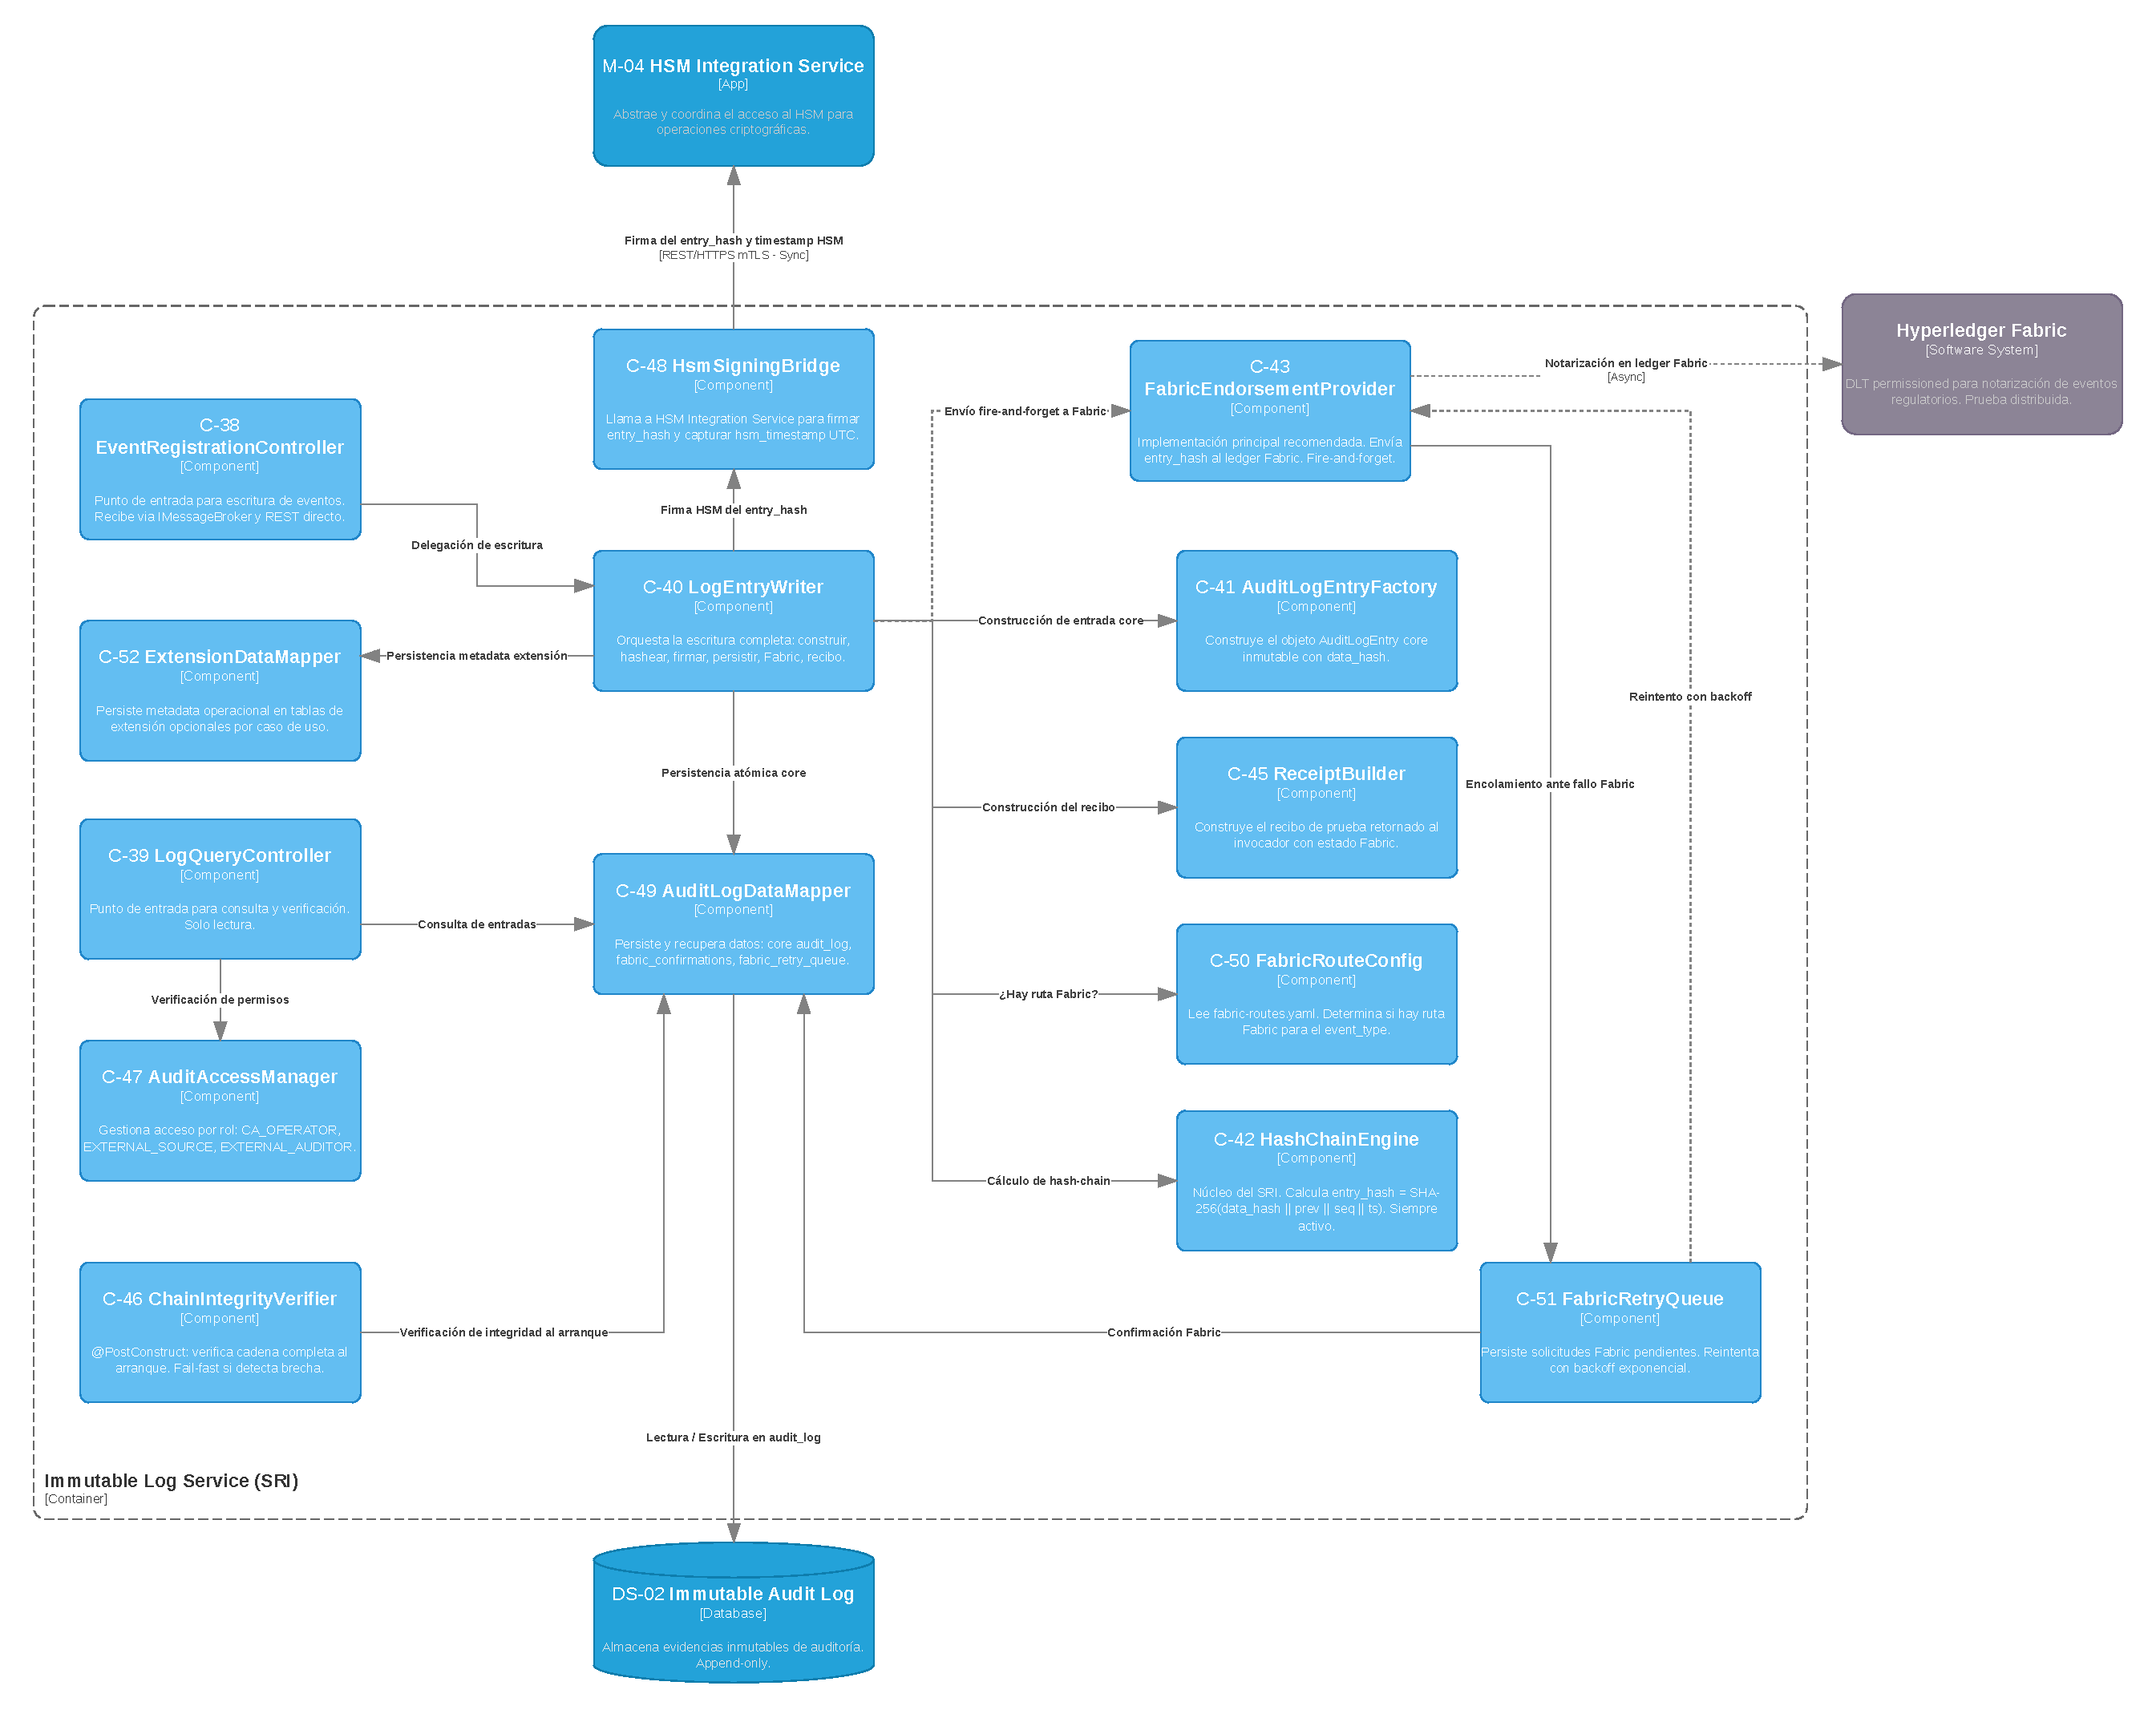
\includegraphics[width=\textwidth]{figs/resultados/m05-c4-nv3.pdf}
\caption[C4 N3: M-05 Immutable Log Service]{Diagrama de componentes del contenedor M-05 Immutable Log Service (ILS).}
\label{fig:c4_n3_m05}
\end{figure}

El motor de hash-encadenado (\texttt{HashChainEngine}) es el núcleo estructural del
contenedor: calcula
$\mathit{entry\_hash} = \textup{SHA-256}(\mathit{data\_hash} \| \mathit{prev\_hash} \|
\mathit{seq} \| \mathit{ts})$ para cada entrada, garantizando que cualquier modificación
retroactiva rompa la cadena completa de forma detectable. El verificador de integridad
(\texttt{ChainIntegrityVerifier}) comprueba la cadena completa en el arranque del servicio
con lógica \textit{fail-fast}: el ILS no acepta escrituras si detecta una brecha en la
secuencia. La integración con Hyperledger Fabric se implementa con un patrón
\textit{fire-and-forget} en \texttt{FabricEndorsementProvider}, acompañado de reintentos
gestionados por \texttt{FabricRetryQueue}, evitando que la latencia de la red Fabric afecte
el tiempo de respuesta del registro principal. El puente de firma HSM
(\texttt{HsmSigningBridge}) captura la firma y el \texttt{hsm\_timestamp} UTC para cada
entrada, añadiendo no repudio criptográfico. El acceso al log se gobierna por roles
(\texttt{CA\_OPERATOR}, \texttt{EXTERNAL\_SOURCE} y \texttt{EXTERNAL\_AUDITOR}) a través
del gestor de acceso (\texttt{AuditAccessManager}), separando la escritura y la consulta
en dos controladores con acoplamiento nulo entre sí. La notarización en Fabric complementa
el hash-chain local de PA-05 con una segunda capa de inmutabilidad distribuida, cuya
solidez descansa en la descentralización real de la red y en la independencia entre
sus organizaciones participantes.

% ======================================================================
% 6.3 — PROTOTIPO: MÓDULO DE AUDITORÍA (ILS)
% ======================================================================

\section{Prototipo: Módulo de Auditoría (ILS)}\label{sec:prototipo}

Esta sección presenta el diagrama de implementación del prototipo desarrollado para
validar experimentalmente la capa de auditoría de la arquitectura de referencia. El
Immutable Log Service (ILS) integra un log hash-encadenado en PostgreSQL con
confirmación selectiva de eventos de alta relevancia regulatoria en Hyperledger Fabric,
más un servidor TSA conforme a RFC~3161. Las especificaciones del entorno experimental
(nodos, límites de memoria y versiones de software) se documentan en el
\hyperref[anx:poc_entorno]{Anexo~H}.

% ----------------------------------------------------------------------
\subsection{Implementación: Diagrama de Código (C4 Nivel 4)}\label{subsec:c4_n4}

El Nivel~4 del modelo C4 descompone el módulo ILS hasta el nivel de clase, verificando
la correspondencia entre los componentes definidos en el N3 y las clases implementadas en
el prototipo~\cite{brown2022c4}. El diagrama de clases expone 19 clases distribuidas en
tres grupos funcionales: los controladores de entrada (escritura y consulta), el núcleo de
orquestación y persistencia, y la infraestructura de mensajería asíncrona que implementa
la interfaz \texttt{IMessageBroker} del canal de comunicación M-10.

\begin{figure}[H]
\centering
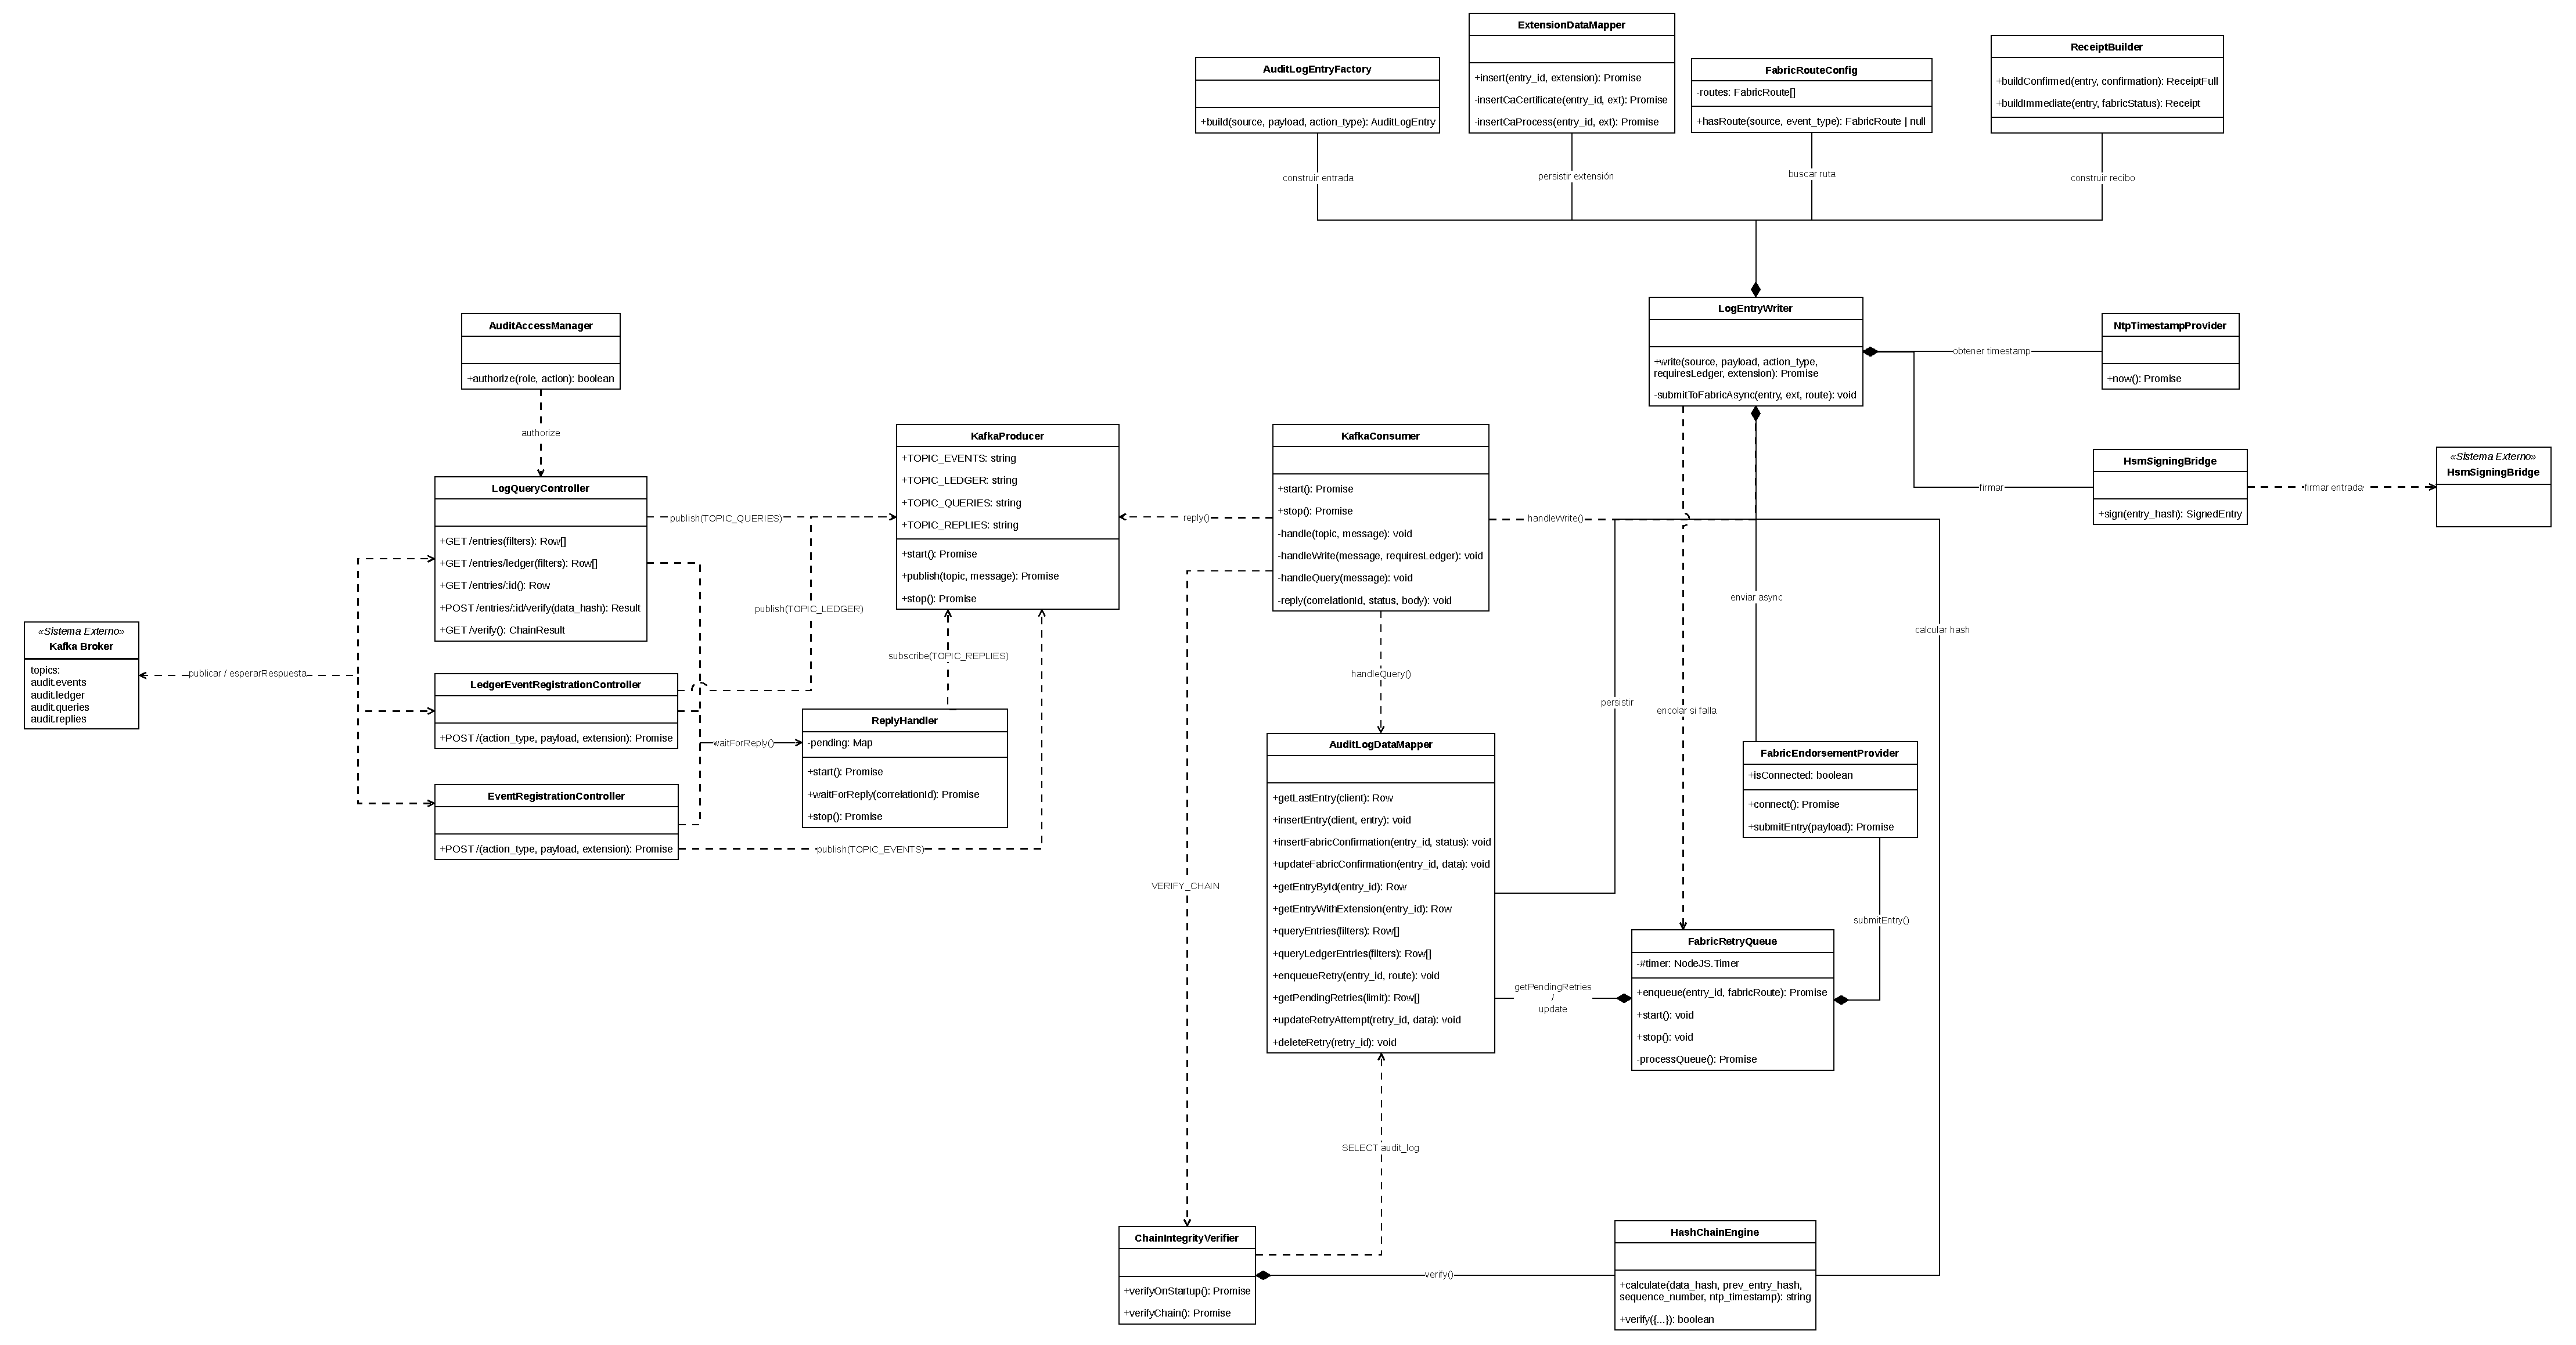
\includegraphics[width=\textwidth]{figs/resultados/class-diagram.pdf}
\caption[C4 N4: M-05 Immutable Log Service]{Diagrama de clases del módulo M-05 Immutable Log Service, correspondiente al Nivel~4 del modelo C4.}
\label{fig:c4_n4}
\end{figure}

El diagrama cumple íntegramente la especificación del N3. Los 14 componentes definidos
 están presentes y correctamente conectados; los adicionales
(\texttt{KafkaProducer}, \texttt{KafkaConsumer}, \texttt{ReplyHandler},
\texttt{LedgerEventRegistrationController} y \texttt{NtpTimestampProvider}) son
realizaciones técnicas de abstracciones del N3: \texttt{KafkaProducer} y
\texttt{KafkaConsumer} materializan el contrato \texttt{IMessageBroker} prescrito por
ADR-31, mientras que \texttt{NtpTimestampProvider} encapsula la fuente de tiempo requerida
por el \texttt{HashChainEngine} sin exponerla como dependencia directa de \texttt{LogEntryWriter}.

El núcleo del diseño es \texttt{LogEntryWriter}, que orquesta ocho componentes mediante
relaciones de composición: \texttt{AuditLogEntryFactory} construye la entrada inmutable,
\texttt{HashChainEngine} calcula el hash de cadena, \texttt{HsmSigningBridge} firma el
\texttt{entry\_hash} y captura el \texttt{hsm\_timestamp} UTC invocando al HSM Integration
Service, \texttt{AuditLogDataMapper} persiste el registro en la base de datos,
\texttt{ExtensionDataMapper}
gestiona los metadatos opcionales por caso de uso, \texttt{FabricRouteConfig} determina
si el evento requiere notarización, \texttt{FabricEndorsementProvider} ejecuta
el envío asíncrono al ledger y \texttt{ReceiptBuilder} construye el recibo devuelto al
invocador.

La resistencia a la incorporación de nuevos módulos se sostiene en tres mecanismos de
diseño independientes. Primero, \texttt{FabricRouteConfig} lee \texttt{fabric-routes.yaml}
en tiempo de arranque: añadir un nuevo módulo como fuente de eventos no requiere modificar
ninguna clase, solo declarar la ruta del nuevo origen en el archivo de configuración.
Segundo, \texttt{ExtensionDataMapper} aísla los metadatos específicos por caso de uso en
métodos privados (\texttt{-insertCaCertificate}, \texttt{-insertCaProcess}): un nuevo
módulo con extensión propia añade un método privado en \texttt{ExtensionDataMapper} y deja
\texttt{LogEntryWriter} sin cambios. Tercero, \texttt{HsmSigningBridge} abstrae la interfaz
con el hardware criptográfico: cualquier cambio de algoritmo o proveedor HSM queda confinado
a M-04 sin que M-05 requiera modificación alguna, satisfaciendo la garantía de alcance
de QAS-14 (crypto-agility).


% ======================================================================
% 6.4 — EVALUACIÓN DE LA ARQUITECTURA Y EL PROTOTIPO
% ======================================================================

\section{Evaluación de la Arquitectura y el Prototipo}\label{sec:evaluacion}

Esta sección presenta los resultados de la evaluación de la arquitectura y el prototipo
mediante dos métodos complementarios. El primero es el experimento GQM, que valida el
comportamiento del módulo ILS mediante seis objetivos de medición y treinta y cinco
preguntas operacionales documentados en el \hyperref[anx:gqm_catalogo]{Anexo~I}. El
segundo es el análisis ATAM, que evalúa la arquitectura de referencia completa a través
del árbol de utilidad, la identificación de riesgos y la detección de compromisos entre
atributos de calidad. Los resultados GQM se presentan en las subsecciones~\ref{subsec:poc_g1g2}
y~\ref{subsec:poc_metricas}; el análisis ATAM se desarrolla en la
subsección~\ref{subsec:atam}.

% ----------------------------------------------------------------------
\subsection{Proceso GQM: Correctitud Funcional (G1--G2)}\label{subsec:poc_g1g2}

La suite GQM se ejecutó el 26 de mayo de 2026 (\texttt{2026-05-26T01:53:59\,UTC}) sobre el
entorno descrito en el \hyperref[anx:poc_entorno]{Anexo~H}, con resultado global de 129
pasos aprobados y 0 fallos en una duración de 162,1\,s. Los objetivos G1 y G2 evalúan
la correctitud funcional del módulo ILS en los dos escenarios de negocio más críticos:
el ciclo de vida completo del certificado (G1) y el firmado electrónico multi-firmante (G2). Para cada objetivo se definen primero las
preguntas operacionales, que delimitan los comportamientos a verificar, y a continuación
el diseño de medición, que establece la métrica exacta y el umbral de aceptación derivado
del NFR asociado. La Tabla~\ref{tab:preguntas_g1} presenta las trece preguntas que
operacionalizan G1, organizadas según el caso de prueba al que corresponden.

\footnotesize
\begin{longtable}{@{}p{0.75cm}p{8.5cm}p{2.5cm}@{}}
\caption{Preguntas operacionales --- G1: Correctitud funcional del ciclo de vida del certificado}\label{tab:preguntas_g1}\\
\toprule
\textbf{ID} & \textbf{Pregunta} & \textbf{Caso de prueba} \\
\midrule
\endfirsthead
\multicolumn{3}{l}{\small\itshape Continuación de la Tabla~\thetable}\\[2pt]
\toprule
\textbf{ID} & \textbf{Pregunta} & \textbf{Caso de prueba} \\
\midrule
\endhead
\bottomrule
\endlastfoot
Q1.1 &
  ¿Se registran en el ILS los eventos operativos de pre-emisión sin generar ningún evento en Fabric? &
  Caso 1, Pasos 1--4 \\
\midrule
Q1.2 &
  ¿Se registra \texttt{CA\_KEY\_GENERATED} en el ILS y se confirma en Fabric? &
  Caso 1, Paso 5 \\
\midrule
Q1.3 &
  ¿Se registra \texttt{CERTIFICATE\_ISSUED} en el ILS con hash encadenado y se confirma en Fabric? &
  Caso 1, Paso 6 \\
\midrule
Q1.4 &
  ¿Se registran en el ILS los eventos de entrega del certificado (P12, descarga, destrucción de clave) sin generar eventos en Fabric? &
  Caso 1, Pasos 7--9 \\
\midrule
Q1.5 &
  ¿Permanece íntegro el hash chain tras las fases de pre-emisión, issuance y entrega? &
  Caso 1, Paso 10 \\
\midrule
Q1.6 &
  ¿Se registra \texttt{CERTIFICATE\_REVOKED} en el ILS y se confirma en Fabric con transacción independiente de la emisión? &
  Caso 1, Paso 11 \\
\midrule
Q1.7 &
  ¿Se registra en el ILS la exportación del log para el auditor externo sin generar evento en Fabric? &
  Caso 1, Paso 12 \\
\midrule
Q1.8 &
  ¿Es posible reconstruir el ciclo completo de un certificado desde PostgreSQL por \texttt{cert\_serial}? &
  Caso 1, Paso 13 \\
\midrule
Q1.9 &
  ¿Permanece íntegro el hash chain al final del ciclo completo de 14 pasos? &
  Caso 1, Paso 14 \\
\midrule
Q1.10 &
  ¿Se registran correctamente todos los eventos del ciclo de renovación con los tres eventos blockchain independientes? &
  Caso 3 \\
\midrule
Q1.11 &
  ¿Se registra y notariza el ciclo completo de revocación de emergencia con solo la revocación en blockchain? &
  Caso 4 \\
\midrule
Q1.12 &
  ¿Queda registrada una solicitud rechazada en el ILS sin generar ningún evento en blockchain, manteniendo la integridad del hash chain? &
  Caso 5 \\
\midrule
Q1.13 &
  ¿Se procesan correctamente 3 certificados en lote con sus 6 eventos blockchain confirmados en Fabric y trazabilidad completa por \texttt{cert\_serial}? &
  Caso 6 \\
\end{longtable}
\normalsize

Las trece preguntas revelan la estructura del experimento: Q1.1 a Q1.9 cubren el ciclo
estándar de catorce pasos (emisión, entrega, revocación, trazabilidad y verificación de
integridad), mientras que Q1.10 a Q1.13 extienden la cobertura a ciclos derivados con
requisitos de confirmación Fabric distintos. Una característica central del diseño es la
selectividad de la notarización: solo tres tipos de evento (generación de clave CA, emisión
y revocación de certificado) generan transacciones en el ledger distribuido; el resto se
registra exclusivamente en el log local del ILS. Esta distinción queda explícita en las
preguntas Q1.1, Q1.4 y Q1.7, que verifican que los eventos operativos ordinarios no
produzcan confirmaciones Fabric innecesarias. Por otra parte, la Tabla~\ref{tab:preguntas_g2} recoge las
cuatro preguntas del objetivo G2, que concentran la evaluación en el escenario de firma
electrónica CAdES-BES con múltiples firmantes.

\footnotesize
\begin{longtable}{@{}p{0.75cm}p{8.5cm}p{2.5cm}@{}}
\caption{Preguntas operacionales --- G2: Correctitud funcional del firmado electrónico}\label{tab:preguntas_g2}\\
\toprule
\textbf{ID} & \textbf{Pregunta} & \textbf{Caso de prueba} \\
\midrule
\endfirsthead
\multicolumn{3}{l}{\small\itshape Continuación de la Tabla~\thetable}\\[2pt]
\toprule
\textbf{ID} & \textbf{Pregunta} & \textbf{Caso de prueba} \\
\midrule
\endhead
\bottomrule
\endlastfoot
Q2.1 &
  ¿Se registra correctamente cada firma individual \texttt{DOCUMENT\_SIGN} con confirmación en Fabric? &
  Caso 2, todos los escenarios \\
\midrule
Q2.2 &
  ¿Escala el sistema de 1 a 5 firmantes sin degradación en la tasa de aceptación? &
  Caso 2 \\
\midrule
Q2.3 &
  ¿La trazabilidad del documento es completa en PostgreSQL para cada escenario de firma? &
  Caso 2 \\
\midrule
Q2.4 &
  ¿El hash chain permanece íntegro después de los 8 eventos \texttt{DOCUMENT\_SIGN} acumulados? &
  Caso 2, verificación final \\
\end{longtable}
\normalsize

G2 es estructuralmente más compacto que G1: las cuatro preguntas verifican un único tipo
de evento (\texttt{DOCUMENT\_SIGN}) bajo tres niveles de concurrencia creciente (1, 2 y 5
firmantes simultáneos), lo que permite evaluar la escalabilidad del registro sin
introducir nuevos tipos de datos en el log. La pregunta Q2.4, que verifica la integridad
del hash chain tras los ocho eventos acumulados del Caso~2, opera sobre el mismo log
que acumuló los eventos de G1, comprobando que ambos objetivos compartan el mismo
sustrato de auditoría sin interferencia. Con las preguntas definidas para G1 y G2, la
Tabla~\ref{tab:gqm_g1_diseno} formaliza el diseño de medición de G1, especificando para
cada grupo de preguntas el foco de verificación, la métrica observable y el umbral de
aceptación.

\footnotesize
\begin{longtable}{@{}p{0.85cm}p{4.2cm}p{3.4cm}p{1.6cm}p{1.5cm}@{}}
\caption{Diseño GQM --- G1: Correctitud funcional del ciclo de vida del certificado}\label{tab:gqm_g1_diseno}\\
\toprule
\textbf{Preg.} & \textbf{Foco de verificación} & \textbf{Métrica} & \textbf{Umbral} & \textbf{ASR} \\
\midrule
\endfirsthead
\multicolumn{5}{l}{\small\itshape Continuación de la Tabla~\thetable}\\[2pt]
\toprule
\textbf{Preg.} & \textbf{Foco de verificación} & \textbf{Métrica} & \textbf{Umbral} & \textbf{ASR} \\
\midrule
\endhead
\bottomrule
\endlastfoot
Q1.1 Q1.4 Q1.7 &
  Registro en ILS-only de eventos operativos sin confirmación Fabric &
  \texttt{fabric\_confirmations} por evento operativo &
  0 confirmaciones &
  NFR-07 QAS-05 \\
\midrule
Q1.2 Q1.3 Q1.6 &
  Confirmación en Hyperledger Fabric de \texttt{CA\_KEY\_GENERATED}, \texttt{CERTIFICATE\_ISSUED} y \texttt{CERTIFICATE\_REVOKED} &
  \textbullet~\texttt{fabric\_status}\newline\textbullet~\texttt{fabric\_tx\_id} &
  \textbullet~CONFIRMED\newline\textbullet~$\neq$ null &
  NFR-07 QAS-05 \\
\midrule
Q1.3 &
  Latencia desde publicación en \texttt{audit.events.ledger} hasta receipt de confirmación Fabric &
  Tiempo hasta confirmación &
  $\leq$\,10\,000\,ms &
  NFR-07 \\
\midrule
Q1.5 Q1.9 &
  Integridad del hash chain tras ciclo completo de catorce pasos (once entries) &
  \textbullet~\texttt{verifyChain().ok}\newline\textbullet~\texttt{entriesChecked} &
  \textbullet~true\newline\textbullet~$\geq$\,11 &
  NFR-07 QAS-05 \\
\midrule
Q1.8 &
  Trazabilidad forense del ciclo de vida por \texttt{cert\_serial} en PostgreSQL &
  \textbullet~ISSUED y REVOKED presentes\newline\textbullet~\texttt{seq(ISSUED)} $<$ \texttt{seq(REVOKED)} &
  Logs en orden cronológico &
  NFR-07 QAS-05 \\
\midrule
Q1.10--Q1.13 &
  Correctitud de ciclos derivados: renovación (3~tx), revocación de emergencia (1~tx), solicitud rechazada (0~tx) y emisión en lote (6~tx) &
  \textbullet~Pasos OK / total\newline\textbullet~Eventos blockchain por ciclo &
  \textbullet~100\,\%\newline\textbullet~0, 1 o 6 según diseño &
  NFR-07 QAS-05 \\
\end{longtable}
\normalsize

El diseño de G1 organiza las trece preguntas en seis grupos de medición según la
dimensión de correctitud que cada uno evalúa. El primer grupo (Q1.1, Q1.4, Q1.7) verifica
el filtro de selectividad: ningún evento operativo debe producir confirmaciones en Fabric.
El segundo grupo (Q1.2, Q1.3, Q1.6) verifica la ruta afirmativa: los tres tipos de evento
de alta relevancia regulatoria deben obtener \texttt{fabric\_status = CONFIRMED} con
\texttt{fabric\_tx\_id} no nulo. La latencia de confirmación Fabric tiene umbral propio
(Q1.3, $\leq$~10\,000\,ms), deliberadamente conservador respecto al tiempo finalmente observado
(3\,002\,ms), para absorber variaciones de red en entornos de producción. Los grupos
restantes verifican integridad del hash chain en puntos de control clave y trazabilidad
forense por número de serie. La Tabla~\ref{tab:gqm_g2_diseno} presenta el diseño
equivalente para G2.

\footnotesize
\begin{longtable}{@{}p{0.85cm}p{4.2cm}p{3.4cm}p{1.6cm}p{1.5cm}@{}}
\caption{Diseño GQM --- G2: Correctitud funcional del firmado electrónico}\label{tab:gqm_g2_diseno}\\
\toprule
\textbf{Preg.} & \textbf{Foco de verificación} & \textbf{Métrica} & \textbf{Umbral} & \textbf{ASR} \\
\midrule
\endfirsthead
\multicolumn{5}{l}{\small\itshape Continuación de la Tabla~\thetable}\\[2pt]
\toprule
\textbf{Preg.} & \textbf{Foco de verificación} & \textbf{Métrica} & \textbf{Umbral} & \textbf{ASR} \\
\midrule
\endhead
\bottomrule
\endlastfoot
Q2.1--Q2.3 &
  Registro y confirmación Fabric de firmas CAdES-BES para 1, 2 y 5 firmantes;
  trazabilidad en PostgreSQL por \texttt{cert\_serial} &
  \textbullet~\texttt{fabric\_status} $\times$~N\newline\textbullet~\texttt{firma\_order} 1\,..\,N &
  \textbullet~CONFIRMED\newline\textbullet~100\,\%\newline\textbullet~orden creciente &
  NFR-07 QAS-05 \\
\midrule
Q2.4 &
  Integridad del hash chain tras ocho eventos \texttt{DOCUMENT\_SIGN} acumulados &
  \textbullet~\texttt{verifyChain().ok}\newline\textbullet~\texttt{entriesChecked} &
  \textbullet~true\newline\textbullet~$\geq$\,19 &
  NFR-07 \\
\end{longtable}
\normalsize

El diseño de G2 consolida sus cuatro preguntas en dos grupos: el primero verifica la
confirmación Fabric de cada firma individual y la trazabilidad por número de serie del
certificado firmante en los tres escenarios de concurrencia; el segundo verifica la
integridad del hash chain tras los ocho eventos \texttt{DOCUMENT\_SIGN} acumulados, con
umbral \texttt{entriesChecked}~$\geq$~19, que refleja la suma de los once entries de G1
más los ocho de G2 hasta ese punto del experimento. La separación en dos grupos de
medición distingue la correctitud del protocolo de confirmación (dependiente de la red
Fabric) de la correctitud del mecanismo de hash-encadenado (local al ILS), permitiendo
diagnosticar fallos en cada dimensión de forma independiente.

La Tabla~\ref{tab:poc_funcionales} resume los seis casos funcionales (G1) y el caso de
firmado electrónico (G2). Todos los ciclos se completaron sin fallos. El tiempo de
confirmación Fabric para \texttt{CERTIFICATE\_ISSUED} fue de 3\,002\,ms (Q1.3;
umbral $\leq$\,10\,000\,ms) y para \texttt{DOCUMENT\_SIGN} el máximo registrado fue de
3\,004\,ms (Q2.1). El verificador de integridad (\texttt{verifyChain()}) confirmó la integridad
del hash chain en todas las verificaciones intermedias y finales.

\begin{table}[H]
\centering
\small
\caption{Resultados de correctitud funcional (G1--G2)}
\label{tab:poc_funcionales}
\begin{tabular}{@{}p{0.5cm}p{3.0cm}p{0.8cm}p{0.8cm}p{6.1cm}@{}}
\toprule
\textbf{G} & \textbf{Suite} & \textbf{PASS} & \textbf{FAIL} & \textbf{Observación} \\
\midrule
G1 & Caso 1 --- Ciclo Estándar & 19 & 0 &
  \textbullet~\texttt{CERTIFICATE\_ISSUED} confirmado en 3\,002\,ms\newline
  \textbullet~\texttt{verifyChain().ok} en chainMid (9 entries) y chainFinal (11 entries) \\
\midrule
G1 & Caso 3 --- Renovación & 16 & 0 &
  \textbullet~3 tx Fabric independientes (CA\_KEY\_GEN, ISSUED, REVOKED)\newline
  \textbullet~\texttt{verifyChain().ok} post-renovación \\
\midrule
G1 & Caso 4 --- Revocación emergencia & 10 & 0 &
  \textbullet~1 tx Fabric (CERTIFICATE\_REVOKED)\newline
  \textbullet~7 eventos ILS-only\newline
  \textbullet~\texttt{verifyChain().ok} post-incidente \\
\midrule
G1 & Caso 5 --- Solicitud rechazada & 8 & 0 &
  \textbullet~0 eventos Fabric\newline
  \textbullet~6 eventos ILS-only\newline
  \textbullet~\texttt{verifyChain().ok} sin ninguna emisión \\
\midrule
G1 & Caso 6 --- Emisión en lote & 32 & 0 &
  \textbullet~20 entries en ILS\newline
  \textbullet~6 tx Fabric (3 CA\_KEY\_GEN + 3 ISSUED)\newline
  \textbullet~\texttt{entriesChecked}\,=\,63 post-lote \\
\midrule
G2 & Caso 2 --- Firmado multi-firma & 31 & 0 &
  \textbullet~8 \texttt{DOCUMENT\_SIGN} confirmados\newline
  \textbullet~Máximo 3\,004\,ms por firma\newline
  \textbullet~\texttt{entriesChecked}\,=\,19 tras Caso~2 \\
\bottomrule
\end{tabular}
\end{table}

Los resultados confirman que todos los ciclos se completaron sin ningún fallo. En la columna
de observaciones, \textit{chainMid} denota una verificación de integridad intermedia ejecutada
con el log parcialmente poblado durante el transcurso del caso de prueba, mientras que
\textit{chainFinal} corresponde a la verificación ejecutada al término del caso con la
totalidad de entries registrados. El término \textit{tx~Fabric} designa un evento de alta
relevancia regulatoria confirmado en el ledger distribuido de Hyperledger Fabric, a
diferencia de los eventos registrados únicamente en el log local del ILS. La selectividad
de la notarización queda reflejada en los casos 4 y 5: la revocación de emergencia genera
una única transacción Fabric mientras registra siete eventos ILS-only; la solicitud rechazada
no produce ninguna transacción en el ledger, preservando así la integridad del hash chain
sin emitir evidencia criptográfica de una operación que no se materializó.

% ----------------------------------------------------------------------
\subsection{Resultados de Métricas por Escenario}\label{subsec:poc_metricas}

Los objetivos G3 a G6 cubren las dimensiones de integridad y control de acceso (G3--G4),
rendimiento bajo carga sostenida (G5) y trazabilidad forense (G6). Su proceso de medición
completo, incluyendo preguntas operacionales y diseño de métricas, se documenta en el
\hyperref[anx:gqm_catalogo]{Anexo~I}; a continuación se presentan los resultados
observados.

\paragraph{G3--G4 --- Integridad y seguridad.}
Las pruebas de seguridad acumularon 8 pasos sin fallos en dos dimensiones complementarias:
la robustez del hash chain frente a modificaciones directas en la base de datos (G3) y el
control de acceso e integridad del receipt de auditoría (G4). La
Tabla~\ref{tab:poc_seguridad} detalla los resultados por métrica.

\small
\begin{longtable}{@{}p{1.4cm}p{4.1cm}p{4.5cm}p{1.0cm}@{}}
\caption{Resultados de integridad y seguridad (G3--G4)}\label{tab:poc_seguridad}\\
\toprule
\textbf{Métrica} & \textbf{Verificación} & \textbf{Resultado observado} & \textbf{Est.} \\
\midrule
\endfirsthead
\multicolumn{4}{l}{\small\itshape Continuación de la Tabla~\thetable}\\[2pt]
\toprule
\textbf{Métrica} & \textbf{Verificación} & \textbf{Resultado observado} & \textbf{Est.} \\
\midrule
\endhead
\bottomrule
\endlastfoot
M3.1.1 &
  Modificación directa de \texttt{data\_hash} mediante \texttt{UPDATE} SQL &
  Aceptada por la base de datos; comportamiento esperado para actor con privilegios de escritura &
  PASS \\
\midrule
M3.2.3 &
  Detección de discrepancia sin consultar Fabric &
  \texttt{entry\_hash} almacenado difiere del \texttt{data\_hash} modificado; corrupción detectable localmente &
  PASS \\
\midrule
M3.3.3 &
  Restauración del valor original &
  Hash chain devuelto a estado íntegro &
  PASS \\
\midrule
M3.4.1 M3.4.2 &
  Localización del \texttt{sequence\_number} corrupto por \texttt{verifyChain()} &
  No aplica por diseño: bloque \texttt{finally} del test restaura el valor antes de cualquier llamada a \texttt{verifyChain()} &
  No aplica \\
\midrule
M4.1.1 &
  Control de acceso: solicitud sin \texttt{X-Audit-Source} &
  Endpoint HTTP responde con código 401 &
  PASS \\
\midrule
M4.2.2 &
  Anti-replay para \textit{payloads} idénticos &
  \texttt{entry\_id} distintos generados para cada solicitud &
  PASS \\
\midrule
M4.3.1 &
  Consistencia entre receipt del servicio y PostgreSQL &
  \texttt{entry\_hash} coincide exactamente &
  PASS \\
\end{longtable}
\normalsize

La protección opera en dos capas: los permisos de solo lectura SQL constituyen la barrera
para clientes de auditoría ordinarios, mientras que el hash chain detecta cualquier
alteración realizada por un actor privilegiado que eluda esa restricción. Las métricas
M3.4.1 y M3.4.2 no aplican por diseño en ejecución nominal (la corrupción activa no es
observable durante la suite porque el bloque \texttt{finally} garantiza la restauración
antes de cualquier verificación de integridad).

\paragraph{G5 --- Rendimiento bajo carga.}
Las pruebas de rendimiento ejecutaron cinco escenarios de estrés con distintos tipos de
carga y volumen de mensajes (burst de emisión, carga sostenida, firma múltiple, revocación
en burst y carga mixta), midiendo la latencia del producer Kafka, la tasa de error y la
tasa de confirmación Fabric en cada uno. La Tabla~\ref{tab:poc_estres} presenta los
resultados.

\begin{table}[H]
\centering
\small
\caption{Resultados de las pruebas de estrés (G5)}
\label{tab:poc_estres}
\begin{tabular}{@{}p{3.0cm}p{0.7cm}p{0.9cm}p{0.9cm}p{0.9cm}p{1.0cm}p{1.0cm}p{1.8cm}p{0.8cm}@{}}
\toprule
\textbf{Escenario} & \textbf{N} &
\textbf{avg} \textbf{(ms)} & \textbf{p95} \textbf{(ms)} & \textbf{p99} \textbf{(ms)} &
\textbf{Error} & \textbf{Fabric} &
\textbf{Throughput} \textbf{(msg/s)} & \textbf{Est.} \\
\midrule
\textit{Umbral} & & $\leq$\,2\,000 & $\leq$\,5\,000 & &
  $\leq$\,5\,\% & $\geq$\,95\,\% & & \\
\midrule
Burst (CERT\_ISSUED) & 50 & 2 & 3 & 3 & 0,0\% & 100,0\% & 4,99 & PASS \\
\midrule
Carga Sostenida & 200 & 2 & 3 & 3 & 0,0\% & 100,0\% & 14,18 & PASS \\
\midrule
Multi-firma (SIGN) & 100 & 4 & 5 & 6 & 0,0\% & 100,0\% & 9,98 & PASS \\
\midrule
Revocación Burst & 50 & 2 & 3 & 4 & 0,0\% & 100,0\% & 4,99 & PASS \\
\midrule
Carga Mixta & 100 & 2 & 3 & 3 & 0,0\% & 100,0\% & 9,97 & PASS \\
\bottomrule
\end{tabular}
\end{table}

Todos los escenarios superaron los cuatro umbrales configurados. La latencia promedio del
producer Kafka se mantuvo entre 2\,ms y 4\,ms, dos órdenes de magnitud por debajo del
umbral de 2\,000\,ms, con p95 máximo de 5\,ms. La tasa de confirmación Fabric alcanzó el
100\,\% en los cinco escenarios. El escenario de carga sostenida (200 mensajes) exhibió el
mayor throughput (14,18\,msg/s). Los eventos \texttt{DOCUMENT\_SIGN} registraron la
latencia más elevada (4\,ms promedio, 5\,ms p95), consistente con el mayor peso
computacional de las operaciones de firma respecto a los eventos de ciclo de vida de
certificados.

Estas latencias miden el canal de mensajería asíncrono, las variables de latencia
asociadas a operaciones criptográficas dentro de hardware HSM físico FIPS~140-2~L3 no
fueron consideradas en la PoC por restricciones de recursos, ya que la adquisición de
dicho hardware supera el alcance académico del proyecto.

\paragraph{G6 --- Trazabilidad forense.}
Las cuatro operaciones de consulta forense se completaron sin fallos, demostrando que la
combinación del log local con el estado confirmado en Fabric es suficiente para reconstruir
el ciclo de vida completo de un certificado sin acceso privilegiado al servicio activo. La
Tabla~\ref{tab:poc_forense} resume los resultados por operación.

\small
\begin{longtable}{@{}p{3.0cm}p{1.2cm}p{5.7cm}p{1.0cm}@{}}
\caption{Resultados de trazabilidad forense (G6)}\label{tab:poc_forense}\\
\toprule
\textbf{Operación} & \textbf{Caso} & \textbf{Resultado observado} & \textbf{Est.} \\
\midrule
\endfirsthead
\multicolumn{4}{l}{\small\itshape Continuación de la Tabla~\thetable}\\[2pt]
\toprule
\textbf{Operación} & \textbf{Caso} & \textbf{Resultado observado} & \textbf{Est.} \\
\midrule
\endhead
\bottomrule
\endlastfoot
Historial por \texttt{cert\_serial} (M6.1.1) &
  Caso~1 &
  \textbullet~5 tipos de evento recuperados (umbral $\geq$\,2)\newline
  \textbullet~\texttt{seq(ISSUED)}\,=\,6 $<$ \texttt{seq(REVOKED)}\,=\,10\newline
  \textbullet~Ambos con \texttt{fabric\_status\,=\,CONFIRMED} &
  PASS \\
\midrule
Vinculación de renovación &
  Caso~3 &
  Serial anterior revocado con \texttt{revocation\_reason:\,superseded} vinculado al nuevo serial emitido &
  PASS \\
\midrule
Consulta por lote de seriales &
  Caso~6 &
  3 entradas \texttt{CERTIFICATE\_ISSUED} recuperadas, una por certificado emitido &
  PASS \\
\midrule
Detección de manipulación post-registro &
  No Aplica &
  Log local y estado Fabric suficientes sin acceso privilegiado al servicio activo &
  PASS \\
\end{longtable}
\normalsize

El Caso~1 reveló el patrón de ciclo de vida completo con cinco tipos de evento, orden
cronológico confirmado y trazabilidad cruzada hacia Fabric para los dos eventos de alta
relevancia regulatoria. La renovación del Caso~3 demostró que la vinculación entre
seriales consecutivos es posible a través del campo \texttt{revocation\_reason}, sin
necesidad de una tabla de relaciones adicional en la base de datos. La emisión en lote
del Caso~6 verificó que la consulta por lote de seriales recupera exactamente una entrada
\texttt{CERTIFICATE\_ISSUED} por certificado, manteniendo la trazabilidad individual
dentro de una operación colectiva. Finalmente, la detección de manipulación post-registro
confirmó que la combinación del log local con el estado Fabric es suficiente para
identificar alteraciones sin requerir acceso privilegiado al servicio activo.

% ======================================================================
% 6.4.3 — ANÁLISIS ATAM
% ======================================================================

% ----------------------------------------------------------------------
\subsection{Análisis ATAM de la Arquitectura de Referencia}\label{subsec:atam}

Esta subsección presenta los resultados de la evaluación estructural de la arquitectura de
referencia mediante el \textit{Architecture Tradeoff Analysis Method}~(ATAM). El análisis
se circunscribe a los once QAS presentados en la subsección~\ref{subsec:nfr}.
Se exponen el Árbol de Utilidad con los QAS priorizados, el
análisis de sensitivity points y tradeoff points, los \textit{risks} identificados, los \textit{non-risks}
formales y un resumen consolidado de hallazgos.

La evaluación contó con la colaboración de dos stakeholders del dominio: un desarrollador de software con experiencia en el dominio y el director de una CA, quienes aportaron perspectivas de la industria en la revisión de los escenarios de calidad y la identificación de trade-offs.

\subsubsection*{Árbol de Utilidad}

Los once QAS del Utility Tree provienen del catálogo operacionalizado en la
Tabla~\ref{tab:qas_core}. La Tabla~\ref{tab:atam_utility_tree}
los organiza por atributo de calidad; las prioridades se expresan como par (importancia
para el negocio, dificultad de evaluación arquitectónica) donde H\,=\,alto y M\,=\,medio.
El Árbol de Utilidad con los QAS del catálogo completo se incluye en el
\hyperref[anx:utility_tree]{Anexo~J}.

\footnotesize
\begin{longtable}{@{}p{2.5cm}p{1.0cm}p{7.0cm}p{1.5cm}@{}}
\caption{Utility Tree --- QAS evaluados por atributo de calidad}\label{tab:atam_utility_tree}\\
\toprule
\textbf{Atributo} & \textbf{QAS} & \textbf{Enunciado resumido} & \textbf{Prioridad} \\
\midrule
\endfirsthead
\multicolumn{4}{l}{\footnotesize\itshape Continuación de la Tabla~\thetable}\\[2pt]
\toprule
\textbf{Atributo} & \textbf{QAS} & \textbf{Enunciado resumido} & \textbf{Prioridad} \\
\midrule
\endhead
\bottomrule
\endlastfoot
Auditabilidad & QAS-05 &
  Hash chain verificable \textit{offline} sin acceso al servidor activo; operaciones
  \texttt{UPDATE}/\texttt{DELETE}/\texttt{PATCH} declaradas en el contrato del ILS = 0 &
  (H,\,H) \\
\midrule
Privacidad & QAS-06 &
  Campos con datos personales identificables en texto claro en el esquema del ILS = 0 &
  (H,\,M) \\
\midrule
Disponibilidad & QAS-09 &
  Arcos de flujo crítico hacia mensajería asíncrona con semántica síncrona o espera = 0;
  arcos de retorno mensajería $\rightarrow$ contenedores críticos = 0 &
  (H,\,H) \\
\midrule
Disponibilidad & QAS-10 &
  Arcos de dependencia directa motor de emisión $\rightarrow$ contenedor de
  revocación/CRL = 0 &
  (H,\,H) \\
\midrule
Disponibilidad & QAS-11 &
  Estado de sesión compartido entre instancias del motor de emisión: no cumple;
  estado de sesión compartido entre instancias del contenedor OCSP: no cumple &
  (H,\,M) \\
\midrule
Disponibilidad & QAS-21 &
  \textit{Endpoints} del repositorio sin \textit{health check} = 0;
  mecanismo de alerta de \texttt{nextUpdate} declarado en el diseño &
  (H,\,M) \\
\midrule
Extensibilidad & QAS-12 &
  Contenedores cuyo diseño requiere cambio para incorporar el nuevo perfil = 0;
  perfiles definidos como constantes dentro del motor de emisión = 0 &
  (H,\,H) \\
\midrule
Modificabilidad & QAS-13 &
  Dependencias del motor hacia implementaciones concretas de perfiles, HSM, ILS
  o mensajería = 0 &
  (H,\,M) \\
\midrule
Modificabilidad & QAS-14 &
  Cambios en el motor de emisión para incorporar Sub-CA = 0; perfil de Sub-CA
  registrado bajo el mismo contrato que cualquier otro perfil &
  (H,\,M) \\
\midrule
Corrección funcional & QAS-19 &
  Caminos donde el motor recibe solicitud sin validación previa del catálogo = 0;
  campos obligatorios de cada perfil regulado declarados en el \textit{schema} del catálogo &
  (H,\,M) \\
\midrule
Consulta pública & QAS-26 &
  Campos estado, fecha de emisión, caducidad y vigencia en toda respuesta = 4/4;
  \textit{endpoint} sin mecanismo de autenticación del cliente &
  (H,\,M) \\
\end{longtable}
\normalsize

De los once QAS evaluados, cuatro reciben la clasificación de máxima prioridad (H,\,H):
QAS-05 (auditabilidad), QAS-09 y QAS-10 (disponibilidad) y QAS-12 (extensibilidad).
Los siete QAS restantes presentan clasificación (H,\,M) y en conjunto, son la base del análisis
de sensitivity points y tradeoff points que se presenta a continuación.

\subsubsection*{Sensitivity Points y Tradeoff Points}
La evaluación identificó ocho sensitivity points y un tradeoff point alineados con los
QAS del Utility Tree; el catálogo completo se documenta en el
\hyperref[anx:atam_sp_tp_risk]{Anexo~K}. La Tabla~\ref{tab:atam_st_risk} presenta los cinco
clasificados como \textit{risk}, detallando el atributo de calidad afectado y el identificador de
\textit{risk} asociado.

\footnotesize
\begin{longtable}{@{}p{0.8cm}p{4.2cm}p{2.1cm}p{1.5cm}p{2.5cm}@{}}
\caption{Sensitivity Points y Tradeoff Points clasificados como \textit{risk}}\label{tab:atam_st_risk}\\
\toprule
\textbf{ID} & \textbf{Descripción resumida} & \textbf{Atributo} & \textbf{QAS} &
  \textbf{Risk} \\
\midrule
\endfirsthead
\multicolumn{5}{l}{\footnotesize\itshape Continuación de la Tabla~\thetable}\\[2pt]
\toprule
\textbf{ID} & \textbf{Descripción resumida} & \textbf{Atributo} & \textbf{QAS} &
  \textbf{Risk} \\
\midrule
\endhead
\bottomrule
\endlastfoot
S10 &
  Inmutabilidad del objeto Memento dependiente de la implementación del adoptante &
  Auditabilidad & QAS-05 & R-NR-E \\
\midrule
S11 &
  Completitud de la cobertura del \texttt{AuditInterceptor}; rutas bypass no
  detectables por la RA &
  Auditabilidad & QAS-05 & R-NR-F \\
\midrule
S17 &
  Aislamiento de esquema de datos personales nominal vs.\ real (LOPDP) &
  Privacidad & QAS-06 & R-NR-I \\
\midrule
T3 &
  Hyperledger Fabric como implementación de \texttt{IAuditLogger}; latencia de
  notarización bajo carga real no validada antes de la PoC &
  \textbullet~Auditabilidad\newline\textbullet~Modificabilidad &
  \textbullet~QAS-05\newline\textbullet~QAS-13 & T3-risk \\
\end{longtable}
\normalsize

Los tres sensitivity points clasificados como \textit{risk} (S10, S11, S17) corresponden a
decisiones cuyas consecuencias no están completamente especificadas por la RA y dependen
de la implementación del adoptante. El tradeoff point (T3) identifica
tensiones estructurales con impacto directo sobre la auditabilidad. La
Tabla~\ref{tab:atam_st_nonrisk} presenta los cinco clasificados como \textit{non-risk}, detallando
el atributo de calidad afectado y el razonamiento que respalda la decisión, el catálogo
completo se documenta en el \hyperref[anx:atam_sp_tp_nonrisk]{Anexo~K}.

\footnotesize
\begin{longtable}{@{}p{0.8cm}p{3.5cm}p{2.0cm}p{1.5cm}p{4.0cm}@{}}
\caption{Sensitivity Points y Tradeoff Points clasificados como \textit{non-risk}}\label{tab:atam_st_nonrisk}\\
\toprule
\textbf{ID} & \textbf{Descripción resumida} & \textbf{Atributo} & \textbf{QAS} &
  \textbf{Razonamiento} \\
\midrule
\endfirsthead
\multicolumn{5}{l}{\footnotesize\itshape Continuación de la Tabla~\thetable}\\[2pt]
\toprule
\textbf{ID} & \textbf{Descripción resumida} & \textbf{Atributo} & \textbf{QAS} &
  \textbf{Razonamiento} \\
\midrule
\endhead
\bottomrule
\endlastfoot
S8 &
  Comunicación asíncrona preferente vía \textit{broker} &
  Disponibilidad & QAS-09 &
  ADR-31 establece el \textit{broker} como canal preferente; la desconexión estructural
  entre productores y consumidores es verificable en el C4~N2 \\
\midrule
S9 &
  \textit{Statelessness} de contenedores de servicio &
  Disponibilidad & QAS-11 &
  QAS-11 documenta la propiedad como verificable; ningún contenedor declara estado de
  sesión compartido entre instancias \\
\midrule
S12 &
  Estabilidad de la interfaz \texttt{IAuditLogger} &
  \textbullet~Auditabilidad\newline\textbullet~Modificabilidad & QAS-13 &
  La interfaz está definida en la RA y es el contrato que habilita la intercambiabilidad
  del \textit{ledger} (ADR-03/ADR-29) \\
\midrule
S13 &
  Estabilidad de la interfaz \texttt{ICertificateProfile} &
  Extensibilidad & QAS-12 &
  Contrato del Microkernel (ADR-08); su estabilidad es una decisión arquitectónica
  explícita, no un riesgo pendiente \\
\midrule
S14 &
  Ausencia de efectos secundarios en la cadena Chain of Responsibility &
  Extensibilidad & QAS-12 &
  ADR-16 establece que cada eslabón es intercambiable; la ausencia de efectos secundarios
  compartidos es consecuencia estructural del patrón \\
\end{longtable}
\normalsize

S8 y S9 se sustentan en propiedades de disponibilidad: la desconexión entre productores
y consumidores es consecuencia del canal asíncrono preferente, y ningún contenedor
declara estado de sesión compartido entre instancias. S12 y S13 corresponden a contratos
de interfaz con estabilidad declarada: \texttt{IAuditLogger} habilita la intercambiabilidad
del ledger e \texttt{ICertificateProfile} es el punto de extensión del catálogo de
perfiles. S14 es consecuencia estructural del patrón Chain of Responsibility, que impide
por construcción efectos secundarios compartidos entre eslabones. Documentar estos
hallazgos previene que revisiones futuras los traten como decisiones pendientes de
análisis.

\subsubsection*{\textit{Risks} Identificados}
En el contexto del ATAM, un \textit{risk} es una decisión arquitectónica potencialmente
problemática: puede ser una decisión no tomada que deja una brecha en el diseño, o una
decisión tomada cuyas consecuencias no están completamente comprendidas. El catálogo
completo de \textit{risks} del análisis se documenta en el
\hyperref[anx:atam_risks]{Anexo~L}; la Tabla~\ref{tab:atam_risks} consolida los cinco
derivados de los QAS descritos en el Utility Tree.

\small
\begin{longtable}{@{}p{1.1cm}p{2.8cm}p{4.2cm}p{1.8cm}p{1.5cm}@{}}
\caption{\textit{Risks} identificados en el análisis ATAM}\label{tab:atam_risks}\\
\toprule
\textbf{ID} & \textbf{Tipo} & \textbf{\textit{Gap} o decisión sin especificar} &
  \textbf{Atributo} & \textbf{QAS} \\
\midrule
\endfirsthead
\multicolumn{5}{l}{\small\itshape Continuación de la Tabla~\thetable}\\[2pt]
\toprule
\textbf{ID} & \textbf{Tipo} & \textbf{\textit{Gap} o decisión sin especificar} &
  \textbf{Atributo} & \textbf{QAS} \\
\midrule
\endhead
\bottomrule
\endlastfoot
R-NR-E &
  \textbullet~Decisión tomada\newline\textbullet~Consecuencias no comprendidas &
  El objeto Memento no tiene \textit{enforcement} de inmutabilidad en la RA;
  depende de la implementación del adoptante &
  Auditabilidad & QAS-05 \\
\midrule
R-NR-F &
  \textbullet~Decisión tomada\newline\textbullet~Consecuencias no comprendidas &
  Rutas de invocación que eludan el \textit{framework} AOP producen operaciones
  no registradas en el ILS; la RA no define un mecanismo de verificación de cobertura &
  Auditabilidad & QAS-05 \\
\midrule
T3-risk &
  \textbullet~Decisión tomada\newline\textbullet~Consecuencias no comprendidas &
  Latencia de notarización en Fabric (\textasciitilde{}500\,ms--2\,s en
  \texttt{test-network}); impacto bajo carga real no comprendido antes de la PoC &
  \textbullet~Auditabilidad\newline\textbullet~Modificabilidad &
  \textbullet~QAS-05\newline\textbullet~QAS-13 \\
\midrule
R-NR-I &
  \textbullet~Decisión tomada\newline\textbullet~Consecuencias no comprendidas &
  El aislamiento de esquema LOPDP es nominal si el adoptante implementa separación de
  tablas sin controles de acceso a nivel de esquema de base de datos ni cifrado en reposo &
  Privacidad & QAS-06 \\
\end{longtable}
\normalsize

T3-risk queda resuelto por los resultados del experimento GQM: la latencia de
confirmación de Fabric se mantuvo dentro del umbral establecido en los cinco escenarios
de carga evaluados (Tabla~\ref{tab:poc_estres}).

\subsubsection*{\textit{Non-Risks} Documentados}
Un \textit{non-risk} es una decisión cuyo valor actual produce un resultado aceptable respaldado
por razonamiento explícito, documentar estos hallazgos previene que revisiones futuras
cuestionen decisiones sin el contexto de evaluación que las respalda. El catálogo
completo se documenta en el \hyperref[anx:atam_nonrisks]{Anexo~M}; la
Tabla~\ref{tab:atam_nonrisks} presenta los dos \textit{non-risks} formales alineados con los QAS
del Utility Tree, con los supuestos de vigencia que el adoptante debe respetar.

\small
\begin{longtable}{@{}p{0.8cm}p{4.5cm}p{1.4cm}p{4.5cm}@{}}
\caption{\textit{Non-Risks} formales documentados en el análisis ATAM}\label{tab:atam_nonrisks}\\
\toprule
\textbf{ID} & \textbf{Decisión arquitectónica} & \textbf{QAS} &
  \textbf{Supuesto de vigencia} \\
\midrule
\endfirsthead
\multicolumn{4}{l}{\small\itshape Continuación de la Tabla~\thetable}\\[2pt]
\toprule
\textbf{ID} & \textbf{Decisión arquitectónica} & \textbf{QAS} &
  \textbf{Supuesto de vigencia} \\
\midrule
\endhead
\bottomrule
\endlastfoot
NR-2 &
  ADR-17: Interceptor (AOP) como mecanismo transversal de auditoría, la lógica de
  auditoría está separada del código de dominio &
  QAS-05 &
  Que el \textit{framework} AOP cubra todos los puntos de entrada declarados y que no
  se introduzcan llamadas directas que lo eludan \\
\midrule
NR-4 &
  ADR-10: \textit{Command} firmado como unidad de auditoría, el
  \textit{CommandProcessor} verifica el estado \texttt{APPROVED} antes de ejecutar &
  QAS-05 &
  Que el \textit{CommandProcessor} no sea modificado para aceptar estados distintos de
  \texttt{APPROVED} y que el \textit{Command} sea la única ruta de invocación de
  operaciones de dominio \\
\end{longtable}
\normalsize

Ambos \textit{non-risks} están vinculados a QAS-05 y dependen de invariantes de implementación
que la RA no puede verificar estructuralmente: la cobertura total del
\textit{framework} AOP y la unicidad de la ruta de invocación a través del
\textit{Command}. Su documentación expresa los supuestos que el adoptante debe respetar
para que la garantía de auditabilidad se mantenga en producción.

\subsubsection*{Interpretación de Hallazgos}

El balance entre \textit{risks} y \textit{non-risks} refleja una arquitectura con garantías estructurales
sólidas en auditabilidad y disponibilidad. Los cuatro \textit{risks} identificados son decisiones
tomadas con consecuencias no completamente comprendidas, mitigables mediante restricciones
de implementación o mediante los resultados experimentales de la PoC.

R-NR-E y R-NR-F se controlan mediante restricciones de implementación documentadas en
los ADRs correspondientes. R-NR-I depende de que el adoptante implemente controles de
acceso a nivel de esquema de base de datos, incluyendo cifrado en reposo a nivel de motor
de base de datos como parte de los controles mínimos requeridos por PA-08 (LOPDP);
T3-risk queda resuelto con los resultados experimentales de la PoC.

    \chapter{Conclusiones}
\label{cap:conclusiones}

El presente trabajo tuvo como objetivo el diseño de una arquitectura de referencia para
Autoridades de Certificación reguladas bajo el marco legal ecuatoriano, orientada a superar
las limitaciones de rigidez, acoplamiento fuerte y baja escalabilidad de los sistemas PKI
tradicionales. El proceso comprendió cuatro fases: análisis de requisitos normativos y
funcionales, diseño de la arquitectura con el modelo C4 bajo TOGAF ADM, implementación de
una prueba de concepto del módulo de auditoría con Hyperledger Fabric, y evaluación mediante
el experimento GQM y el análisis ATAM. Los hallazgos de cada fase se sintetizan a continuación.

El análisis de los estándares PKI (X.509, RFC~5280, RFC~6960, RFC~3161) y del marco
regulatorio ecuatoriano encabezado por la Resolución ARCOTEL-2024-0176 permitió derivar
una cadena de requisitos que parte de los conductores de negocio y desciende hasta
escenarios de atributo de calidad verificables. Los seis business drivers más destacados
(Tabla~\ref{tab:bd_nfr_core}) se descompusieron en los doce NFRs y once QAS más
relevantes para el diseño (Tablas~\ref{tab:nfr_core} y~\ref{tab:qas_core}). El ejercicio confirmó que
la regulación vigente impone restricciones determinantes sobre la arquitectura: la exigencia
de respuesta OCSP inmediata tras revocación y el almacenamiento de claves exclusivamente en
HSM certificado hacen inviables los estilos de arquitectura con consistencia eventual o sin
aislamiento criptográfico de hardware. Estas restricciones se formalizaron en la
Tabla~\ref{tab:restricciones_arq} y constituyeron el filtro principal para la selección del
estilo arquitectónico. 

Con esos requisitos como marco, la evaluación sistemática de nueve estilos arquitectónicos
frente a diez criterios ponderados (Figura~\ref{fig:estilos_chart}) derivó en la selección
del estilo compuesto EA-10: Service-Based como base, complementado con asincronía selectiva
tomada de Event-Driven Architecture y extensibilidad basada en el patrón Microkernel.
Service-Based fue el único estilo con cero evaluaciones negativas, satisfaciendo los seis
criterios de peso alto y presentando solo resultado parcial en gestión de carga; esta
limitación se subsanó con la incorporación del broker de mensajería asíncrono (ADR-27,
ADR-31). La arquitectura resultante se materializa en diez contenedores de grano grueso
(Figura~\ref{fig:c4_n2} y Tabla~\ref{tab:contenedores}), cada uno con responsabilidad
delimitada por al menos una decisión arquitectónica documentada en el ADR Log. Los treinta
y nueve ADRs agrupados en seis categorías (Tabla~\ref{tab:adrs_core} y Anexo~G) formalizan
la justificación de cada decisión de diseño, vinculándola con los NFRs y QAS que la motivan
y con las métricas que la validan. Entre estas, la restricción de acoplamiento eferente
Ce~$\leq$~5 por contenedor (ADR-33), verificable directamente en los diagramas C4 de
Nivel~3, constituye una métrica objetiva que permite auditar el grado de independencia entre
contenedores sin herramientas de análisis estático externas.

Sobre esa base, la implementación del prototipo materializó esas decisiones en el módulo M-05 Immutable
Log Service. El módulo se descompone en 19 clases organizadas en tres grupos
funcionales: los controladores de entrada para escritura y consulta, el núcleo de
orquestación y persistencia centrado en \texttt{LogEntryWriter}, y la infraestructura de
mensajería asíncrona que implementa el contrato \texttt{IMessageBroker} del canal M-10. Las
decisiones de diseño más determinantes de la implementación son tres. Primero,
\texttt{HashChainEngine} opera siempre activo e independiente de la configuración de Fabric,
garantizando la integridad local del log por construcción y no por convención. Segundo,
\texttt{FabricRouteConfig} separa la política de notarización del código: añadir un nuevo
origen de eventos al ledger distribuido requiere solo una entrada en
\texttt{fabric-routes.yaml}, sin modificar ninguna clase. Tercero, \texttt{HsmSigningBridge}
abstrae la interfaz con el hardware criptográfico de M-04, confinando cualquier cambio de
algoritmo o proveedor a ese contenedor sin afectar a M-05.

La validez de este prototipo fue evaluada con el
experimento GQM descrito en el \hyperref[anx:poc_entorno]{Anexo~H}. Los resultados
confirman tres propiedades estructurales del diseño. En primer lugar, la selectividad de la
notarización es correcta: solo los eventos de alta relevancia regulatoria generan
transacciones en Hyperledger Fabric, mientras que el resto se registra exclusivamente en
el log local, sin que esta distinción comprometa la integridad del hash chain ni la
completitud de la trazabilidad por número de serie (Tabla~\ref{tab:poc_funcionales}).
En segundo lugar, la integración asíncrona con Fabric no degrada el rendimiento del canal de
mensajería bajo ninguno de los cinco escenarios de carga evaluados, lo que confirma la
viabilidad del patrón \textit{fire-and-forget} adoptado en ADR-29
(Tabla~\ref{tab:poc_estres}); la latencia de operaciones criptográficas en hardware HSM
físico queda fuera del alcance de esta PoC por restricciones económicas de adquisición.
En tercer lugar, la protección del log opera en capas
independientes: el hash chain detecta cualquier alteración retroactiva sin necesidad de
consultar el ledger, y el control de acceso rechaza solicitudes no autorizadas antes de
que alcancen el mecanismo criptográfico (Tabla~\ref{tab:poc_seguridad}). La combinación
de estas tres propiedades permite reconstruir el ciclo de vida completo de un certificado
y auditar operaciones en lote (Tabla~\ref{tab:poc_forense}).

De igual manera, el análisis ATAM examinó la arquitectura de referencia en su conjunto
(Tablas~\ref{tab:atam_utility_tree},~\ref{tab:atam_st_risk} y~\ref{tab:atam_st_nonrisk})
e identificó dos categorías de hallazgos diferenciadas. En los puntos donde la arquitectura
fija la decisión de forma estructural (estabilidad de las interfaces de extensibilidad,
aislamiento de flujos críticos respecto a la mensajería asíncrona, ausencia de estado
compartido entre instancias de servicio), las consecuencias son completamente comprendidas y
aceptables: la arquitectura de referencia garantiza esas propiedades por construcción, con
independencia del adoptante. En contraste, las brechas más relevantes
(Tabla~\ref{tab:atam_risks}) se concentran en decisiones que la arquitectura necesariamente
delega al adoptante: la completitud del registro de auditoría ante rutas de invocación que
puedan eludir el mecanismo transversal de intercepción, y la efectividad del aislamiento de
datos personales a nivel de control de acceso en la base de datos. En ambos casos, la arquitectura de referencia prescribe el
mecanismo correcto pero no puede verificar por construcción que la implementación concreta
del adoptante lo respete; esta distinción entre garantía arquitectónica y garantía de
implementación delimita el alcance de las propiedades que una arquitectura de referencia
puede ofrecer. La incertidumbre sobre la latencia de Fabric como implementación del ledger
de auditoría, identificada por el ATAM, queda resuelta por los resultados del experimento (Tabla~\ref{tab:poc_estres}): la
latencia de confirmación observada se mantuvo dentro del umbral establecido en todos los
escenarios evaluados.

Como resultado final, la arquitectura de referencia resultante constituye una especificación formal, trazable y
portable para Autoridades de Certificación que operen bajo el marco regulatorio ecuatoriano.
A diferencia de adaptaciones de plataformas internacionales sin ajuste normativo, esta
propuesta parte de los mandatos legales como restricciones de primer nivel
(Tabla~\ref{tab:restricciones_arq}) y los transforma en decisiones de diseño auditables
mediante el catálogo de ADRs (Anexo~G), los principios arquitectónicos
(Tabla~\ref{tab:principios_inline}) y los diagramas C4 en cuatro niveles de abstracción
(Figuras~\ref{fig:c4_n1} a~\ref{fig:c4_n4}). Una CA adoptante puede verificar cada decisión
contra su contexto regulatorio, sustituir los componentes de terceros por alternativas
conformes a los estándares prescritos (PKCS\#11, RFC~6960, RFC~3161) e incorporar nuevos
perfiles de certificado normativos sin rediseñar el motor de emisión. Esta capacidad de
adopción graduada, posibilitada por la separación entre estándares prescritos e
implementaciones elegibles, constituye la contribución estructural de la propuesta al
ecosistema ecuatoriano regulado de infraestructura de clave pública.

Finalmente, como líneas de trabajo futuro, la validación experimental puede extenderse a
los nueve módulos restantes de la arquitectura siguiendo el mismo proceso GQM aplicado al
módulo de auditoría, con especial atención al motor de emisión y al servicio de validación
OCSP, cuyos atributos de latencia y disponibilidad bajo carga determinan el cumplimiento
de los requisitos de mayor criticidad regulatoria. La integración con HSM físico
FIPS~140-2~L3 permitiría además completar la validación de rendimiento de extremo a
extremo, condicionada al coste de adquisición del hardware. El modelado e implementación 
completa de CA Core Service deberá incorporar además un
control estricto del ciclo de vida de variables sensibles en memoria volátil, línea de
trabajo identificada en R-NR-J. En el plano normativo,
si la regulación ecuatoriana evoluciona para permitir la generación del par de claves en
dispositivo del suscriptor, CA Core Service debería adaptarse para aceptar
solicitudes de firma de certificado (CSR) en lugar de desencadenar la generación
centralizada, lo que permitiría fortalecer la garantía de no repudio en sentido estricto.
Por último, la aplicación de la arquitectura en un proceso formal de acreditación ante
ARCOTEL proporcionaría evidencia empírica sobre la completitud de la cobertura regulatoria
en condiciones de producción.

    % Bibliografía
    \cleardoublepage
    \bibliographystyle{etc/IEEEtranEC}
    % \nocite{*}  % Muestra TODAS las referencias (quitar cuando uses \cite{})
    \bibliography{sections/bibliografia}

    \chapter*{Anexos}\label{cap:anexos}
\phantomsection
\addcontentsline{toc}{chapter}{Anexos}

% ======================================================================
% ANEXO A — CATÁLOGO COMPLETO DE EPICs
% ======================================================================

\section*{Anexo A — Catálogo Completo de EPICs}\label{anx:backlog_completo}
\phantomsection
\addcontentsline{toc}{section}{Anexo A — Catálogo Completo de EPICs}

Neque porro quisquam est, qui dolorem ipsum quia dolor sit amet, consectetur, adipisci velit, sed quia non numquam eius modi tempora incidunt ut labore et dolore magnam aliquam quaerat voluptatem. Ut enim ad minima veniam, quis nostrum exercitationem ullam corporis suscipit laboriosam, nisi ut aliquid ex ea commodi consequatur.

\small
\begin{longtable}{@{}p{1cm}p{4.5cm}p{6.5cm}p{1.3cm}@{}}
\caption{Lorem ipsum dolor sit amet, consectetur adipiscing elit.}\label{tab:epics_completo}\\
\toprule
\textbf{EPIC} & \textbf{Nombre} & \textbf{Referencias normativas} & \textbf{MoSCoW} \\
\midrule
\endfirsthead
\multicolumn{4}{l}{\small\itshape Continuación de la Tabla~\thetable}\\[2pt]
\toprule
\textbf{EPIC} & \textbf{Nombre} & \textbf{Referencias normativas} & \textbf{MoSCoW} \\
\midrule
\endhead
\bottomrule
\endlastfoot
Lorem ipsum dolor & Lorem ipsum dolor & Lorem ipsum dolor & Lorem ipsum dolor \\
Lorem ipsum dolor & Lorem ipsum dolor & Lorem ipsum dolor & Lorem ipsum dolor \\
Lorem ipsum dolor & Lorem ipsum dolor & Lorem ipsum dolor & Lorem ipsum dolor \\
Lorem ipsum dolor & Lorem ipsum dolor & Lorem ipsum dolor & Lorem ipsum dolor \\
Lorem ipsum dolor & Lorem ipsum dolor & Lorem ipsum dolor & Lorem ipsum dolor \\
Lorem ipsum dolor & Lorem ipsum dolor & Lorem ipsum dolor & Lorem ipsum dolor \\
Lorem ipsum dolor & Lorem ipsum dolor & Lorem ipsum dolor & Lorem ipsum dolor \\
Lorem ipsum dolor & Lorem ipsum dolor & Lorem ipsum dolor & Lorem ipsum dolor \\
Lorem ipsum dolor & Lorem ipsum dolor & Lorem ipsum dolor & Lorem ipsum dolor \\
Lorem ipsum dolor & Lorem ipsum dolor & Lorem ipsum dolor & Lorem ipsum dolor \\
Lorem ipsum dolor & Lorem ipsum dolor & Lorem ipsum dolor & Lorem ipsum dolor \\
Lorem ipsum dolor & Lorem ipsum dolor & Lorem ipsum dolor & Lorem ipsum dolor \\
\end{longtable}
\normalsize

At vero eos et accusamus et iusto odio dignissimos ducimus qui blanditiis praesentium voluptatum deleniti atque corrupti quos dolores et quas molestias excepturi sint occaecati cupiditate non provident.

\paragraph{Ut enim ad minima veniam, quis nostrum exercitationem.}
Duis aute irure dolor in reprehenderit in voluptate velit esse cillum dolore eu fugiat nulla pariatur. Excepteur sint occaecat cupidatat non proident, sunt in culpa qui officia deserunt mollit anim id est laborum. Nemo enim ipsam voluptatem quia voluptas sit aspernatur aut odit aut fugit, sed quia consequuntur magni dolores eos qui ratione voluptatem sequi nesciunt. Ut enim ad minima veniam, quis nostrum exercitationem ullam corporis suscipit laboriosam, nisi ut aliquid ex ea commodi consequatur. Quis autem vel eum iure reprehenderit qui in ea voluptate velit esse quam nihil molestiae consequatur, vel illum qui dolorem eum fugiat quo voluptas nulla pariatur.

\paragraph{Et harum quidem rerum facilis est et expedita.}
Et harum quidem rerum facilis est et expedita distinctio, nam libero tempore, cum soluta nobis est eligendi optio cumque nihil impedit quo minus id quod maxime placeat facere possimus. Temporibus autem quibusdam et aut officiis debitis aut rerum necessitatibus saepe eveniet ut et voluptates repudiandae sint et molestiae non recusandae. Ut enim ad minim veniam, quis nostrud exercitation ullamco laboris nisi ut aliquip ex ea commodo consequat. Excepteur sint occaecat cupidatat non proident, sunt in culpa qui officia deserunt mollit anim id est laborum. Nemo enim ipsam voluptatem quia voluptas sit aspernatur aut odit aut fugit, sed quia consequuntur magni dolores eos qui ratione voluptatem sequi nesciunt.

\paragraph{Lorem ipsum dolor sit amet, consectetur adipiscing elit.}
Temporibus autem quibusdam et aut officiis debitis aut rerum necessitatibus saepe eveniet ut et voluptates repudiandae sint et molestiae non recusandae. Lorem ipsum dolor sit amet, consectetur adipiscing elit, sed do eiusmod tempor incididunt ut labore et dolore magna aliqua. Duis aute irure dolor in reprehenderit in voluptate velit esse cillum dolore eu fugiat nulla pariatur. Sed ut perspiciatis unde omnis iste natus error sit voluptatem accusantium doloremque laudantium, totam rem aperiam eaque ipsa quae ab illo inventore veritatis. Nemo enim ipsam voluptatem quia voluptas sit aspernatur aut odit aut fugit, sed quia consequuntur magni dolores eos qui ratione voluptatem sequi nesciunt. Neque porro quisquam est, qui dolorem ipsum quia dolor sit amet, consectetur, adipisci velit, sed quia non numquam eius modi tempora incidunt ut labore et dolore magnam aliquam quaerat voluptatem.

\paragraph{Nemo enim ipsam voluptatem quia voluptas sit aspernatur.}
Excepteur sint occaecat cupidatat non proident, sunt in culpa qui officia deserunt mollit anim id est laborum. Nemo enim ipsam voluptatem quia voluptas sit aspernatur aut odit aut fugit, sed quia consequuntur magni dolores eos qui ratione voluptatem sequi nesciunt. Ut enim ad minima veniam, quis nostrum exercitationem ullam corporis suscipit laboriosam, nisi ut aliquid ex ea commodi consequatur. Quis autem vel eum iure reprehenderit qui in ea voluptate velit esse quam nihil molestiae consequatur, vel illum qui dolorem eum fugiat quo voluptas nulla pariatur. At vero eos et accusamus et iusto odio dignissimos ducimus qui blanditiis praesentium voluptatum deleniti atque corrupti quos dolores et quas molestias excepturi sint occaecati cupiditate non provident.

\paragraph{Nemo enim ipsam voluptatem quia voluptas sit aspernatur.}
Et harum quidem rerum facilis est et expedita distinctio, nam libero tempore, cum soluta nobis est eligendi optio cumque nihil impedit quo minus id quod maxime placeat facere possimus. Lorem ipsum dolor sit amet, consectetur adipiscing elit, sed do eiusmod tempor incididunt ut labore et dolore magna aliqua. Duis aute irure dolor in reprehenderit in voluptate velit esse cillum dolore eu fugiat nulla pariatur. Excepteur sint occaecat cupidatat non proident, sunt in culpa qui officia deserunt mollit anim id est laborum. Sed ut perspiciatis unde omnis iste natus error sit voluptatem accusantium doloremque laudantium, totam rem aperiam eaque ipsa quae ab illo inventore veritatis. Nemo enim ipsam voluptatem quia voluptas sit aspernatur aut odit aut fugit, sed quia consequuntur magni dolores eos qui ratione voluptatem sequi nesciunt.

\paragraph{Duis aute irure dolor in reprehenderit in voluptate.}
Duis aute irure dolor in reprehenderit in voluptate velit esse cillum dolore eu fugiat nulla pariatur. Excepteur sint occaecat cupidatat non proident, sunt in culpa qui officia deserunt mollit anim id est laborum. Sed ut perspiciatis unde omnis iste natus error sit voluptatem accusantium doloremque laudantium, totam rem aperiam eaque ipsa quae ab illo inventore veritatis. Nemo enim ipsam voluptatem quia voluptas sit aspernatur aut odit aut fugit, sed quia consequuntur magni dolores eos qui ratione voluptatem sequi nesciunt. Neque porro quisquam est, qui dolorem ipsum quia dolor sit amet, consectetur, adipisci velit, sed quia non numquam eius modi tempora incidunt ut labore et dolore magnam aliquam quaerat voluptatem.

\paragraph{Temporibus autem quibusdam et aut officiis debitis aut.}
Sed ut perspiciatis unde omnis iste natus error sit voluptatem accusantium doloremque laudantium, totam rem aperiam eaque ipsa quae ab illo inventore veritatis. Nemo enim ipsam voluptatem quia voluptas sit aspernatur aut odit aut fugit, sed quia consequuntur magni dolores eos qui ratione voluptatem sequi nesciunt. Ut enim ad minima veniam, quis nostrum exercitationem ullam corporis suscipit laboriosam, nisi ut aliquid ex ea commodi consequatur. At vero eos et accusamus et iusto odio dignissimos ducimus qui blanditiis praesentium voluptatum deleniti atque corrupti quos dolores et quas molestias excepturi sint occaecati cupiditate non provident.

\paragraph{Ut enim ad minim veniam, quis nostrud exercitation.}
Temporibus autem quibusdam et aut officiis debitis aut rerum necessitatibus saepe eveniet ut et voluptates repudiandae sint et molestiae non recusandae. Lorem ipsum dolor sit amet, consectetur adipiscing elit, sed do eiusmod tempor incididunt ut labore et dolore magna aliqua. Ut enim ad minim veniam, quis nostrud exercitation ullamco laboris nisi ut aliquip ex ea commodo consequat. Duis aute irure dolor in reprehenderit in voluptate velit esse cillum dolore eu fugiat nulla pariatur. Excepteur sint occaecat cupidatat non proident, sunt in culpa qui officia deserunt mollit anim id est laborum. Nemo enim ipsam voluptatem quia voluptas sit aspernatur aut odit aut fugit, sed quia consequuntur magni dolores eos qui ratione voluptatem sequi nesciunt.

\paragraph{Temporibus autem quibusdam et aut officiis debitis aut.}
Ut enim ad minima veniam, quis nostrum exercitationem ullam corporis suscipit laboriosam, nisi ut aliquid ex ea commodi consequatur. Quis autem vel eum iure reprehenderit qui in ea voluptate velit esse quam nihil molestiae consequatur, vel illum qui dolorem eum fugiat quo voluptas nulla pariatur. At vero eos et accusamus et iusto odio dignissimos ducimus qui blanditiis praesentium voluptatum deleniti atque corrupti quos dolores et quas molestias excepturi sint occaecati cupiditate non provident.

\paragraph{Lorem ipsum dolor sit amet, consectetur adipiscing elit.}
Nemo enim ipsam voluptatem quia voluptas sit aspernatur aut odit aut fugit, sed quia consequuntur magni dolores eos qui ratione voluptatem sequi nesciunt. Neque porro quisquam est, qui dolorem ipsum quia dolor sit amet, consectetur, adipisci velit, sed quia non numquam eius modi tempora incidunt ut labore et dolore magnam aliquam quaerat voluptatem. Ut enim ad minima veniam, quis nostrum exercitationem ullam corporis suscipit laboriosam, nisi ut aliquid ex ea commodi consequatur. Quis autem vel eum iure reprehenderit qui in ea voluptate velit esse quam nihil molestiae consequatur, vel illum qui dolorem eum fugiat quo voluptas nulla pariatur.

\paragraph{Nemo enim ipsam voluptatem quia voluptas sit aspernatur.}
Et harum quidem rerum facilis est et expedita distinctio, nam libero tempore, cum soluta nobis est eligendi optio cumque nihil impedit quo minus id quod maxime placeat facere possimus. Temporibus autem quibusdam et aut officiis debitis aut rerum necessitatibus saepe eveniet ut et voluptates repudiandae sint et molestiae non recusandae. Lorem ipsum dolor sit amet, consectetur adipiscing elit, sed do eiusmod tempor incididunt ut labore et dolore magna aliqua. Ut enim ad minim veniam, quis nostrud exercitation ullamco laboris nisi ut aliquip ex ea commodo consequat. Excepteur sint occaecat cupidatat non proident, sunt in culpa qui officia deserunt mollit anim id est laborum. Sed ut perspiciatis unde omnis iste natus error sit voluptatem accusantium doloremque laudantium, totam rem aperiam eaque ipsa quae ab illo inventore veritatis.

\paragraph{Lorem ipsum dolor sit amet, consectetur adipiscing elit.}
Duis aute irure dolor in reprehenderit in voluptate velit esse cillum dolore eu fugiat nulla pariatur. Sed ut perspiciatis unde omnis iste natus error sit voluptatem accusantium doloremque laudantium, totam rem aperiam eaque ipsa quae ab illo inventore veritatis. Nemo enim ipsam voluptatem quia voluptas sit aspernatur aut odit aut fugit, sed quia consequuntur magni dolores eos qui ratione voluptatem sequi nesciunt. Ut enim ad minima veniam, quis nostrum exercitationem ullam corporis suscipit laboriosam, nisi ut aliquid ex ea commodi consequatur. At vero eos et accusamus et iusto odio dignissimos ducimus qui blanditiis praesentium voluptatum deleniti atque corrupti quos dolores et quas molestias excepturi sint occaecati cupiditate non provident.

% ======================================================================
% ANEXO B — BUSINESS DRIVERS
% ======================================================================

\cleardoublepage
\section*{Anexo B --- Business Drivers}\label{anx:business_drivers}
\phantomsection
\addcontentsline{toc}{section}{Anexo B --- Business Drivers}

At vero eos et accusamus et iusto odio dignissimos ducimus qui blanditiis praesentium voluptatum deleniti atque corrupti quos dolores et quas molestias excepturi sint occaecati cupiditate non provident. Et harum quidem rerum facilis est et expedita distinctio, nam libero tempore, cum soluta nobis est eligendi optio cumque nihil impedit quo minus id quod maxime placeat facere possimus. Lorem ipsum dolor sit amet, consectetur adipiscing elit, sed do eiusmod tempor incididunt ut labore et dolore magna aliqua.

\small
\begin{longtable}{@{}p{0.8cm}p{5.4cm}p{2.1cm}p{3.9cm}@{}}
\caption{Quis autem vel eum iure reprehenderit qui in.}\label{tab:business_drivers}\\
\toprule
\textbf{BD} & \textbf{Driver} & \textbf{Tipo} & \textbf{Fuente normativa} \\
\midrule
\endfirsthead
\multicolumn{4}{l}{\small\itshape Continuación de la Tabla~\thetable}\\[2pt]
\toprule
\textbf{BD} & \textbf{Driver} & \textbf{Tipo} & \textbf{Fuente normativa} \\
\midrule
\endhead
\bottomrule
\endlastfoot
Lorem ipsum dolor & Lorem ipsum dolor & Lorem ipsum dolor & Lorem ipsum dolor \\
\midrule
Lorem ipsum dolor & Lorem ipsum dolor & Lorem ipsum dolor & Lorem ipsum dolor \\
\midrule
Lorem ipsum dolor & Lorem ipsum dolor & Lorem ipsum dolor & Lorem ipsum dolor \\
\midrule
Lorem ipsum dolor & Lorem ipsum dolor & Lorem ipsum dolor & Lorem ipsum dolor \\
\midrule
Lorem ipsum dolor & Lorem ipsum dolor & Lorem ipsum dolor & Lorem ipsum dolor \\
\midrule
Lorem ipsum dolor & Lorem ipsum dolor & Lorem ipsum dolor & Lorem ipsum dolor \\
\midrule
Lorem ipsum dolor & Lorem ipsum dolor & Lorem ipsum dolor & Lorem ipsum dolor \\
\midrule
Lorem ipsum dolor & Lorem ipsum dolor & Lorem ipsum dolor & Lorem ipsum dolor \\
\end{longtable}
\normalsize

% ======================================================================
% ANEXO C — CATÁLOGO COMPLETO DE NFRs
% ======================================================================

\cleardoublepage
\section*{Anexo C — Catálogo Completo de NFRs}\label{anx:nfr_completo}
\phantomsection
\addcontentsline{toc}{section}{Anexo C — Catálogo Completo de NFRs}

Ut enim ad minima veniam, quis nostrum exercitationem ullam corporis suscipit laboriosam, nisi ut aliquid ex ea commodi consequatur. Quis autem vel eum iure reprehenderit qui in ea voluptate velit esse quam nihil molestiae consequatur, vel illum qui dolorem eum fugiat quo voluptas nulla pariatur. At vero eos et accusamus et iusto odio dignissimos ducimus qui blanditiis praesentium voluptatum deleniti atque corrupti quos dolores et quas molestias excepturi sint occaecati cupiditate non provident.

\small
\begin{longtable}{@{}p{1cm}p{3.8cm}p{3cm}p{3.5cm}p{1.2cm}@{}}
\caption{Ut enim ad minim veniam, quis nostrud exercitation.}\label{tab:nfr_apendice}\\
\toprule
\textbf{ID} & \textbf{Nombre} & \textbf{Sub-caract. ISO~25010} & \textbf{Valor objetivo} & \textbf{MoSCoW} \\
\midrule
\endfirsthead
\multicolumn{5}{l}{\small\itshape Continuación de la Tabla~\thetable}\\[2pt]
\toprule
\textbf{ID} & \textbf{Nombre} & \textbf{Sub-caract. ISO~25010} & \textbf{Valor objetivo} & \textbf{MoSCoW} \\
\midrule
\endhead
\bottomrule
\endlastfoot
Lorem ipsum dolor & Lorem ipsum dolor & Lorem ipsum dolor & Lorem ipsum dolor & Lorem ipsum dolor \\
\midrule
Lorem ipsum dolor & Lorem ipsum dolor & Lorem ipsum dolor & Lorem ipsum dolor & Lorem ipsum dolor \\
\midrule
Lorem ipsum dolor & Lorem ipsum dolor & Lorem ipsum dolor & Lorem ipsum dolor & Lorem ipsum dolor \\
\midrule
Lorem ipsum dolor & Lorem ipsum dolor & Lorem ipsum dolor & Lorem ipsum dolor & Lorem ipsum dolor \\
\midrule
Lorem ipsum dolor & Lorem ipsum dolor & Lorem ipsum dolor & Lorem ipsum dolor & Lorem ipsum dolor \\
\midrule
Lorem ipsum dolor & Lorem ipsum dolor & Lorem ipsum dolor & Lorem ipsum dolor & Lorem ipsum dolor \\
\midrule
Lorem ipsum dolor & Lorem ipsum dolor & Lorem ipsum dolor & Lorem ipsum dolor & Lorem ipsum dolor \\
\midrule
Lorem ipsum dolor & Lorem ipsum dolor & Lorem ipsum dolor & Lorem ipsum dolor & Lorem ipsum dolor \\
\midrule
Lorem ipsum dolor & Lorem ipsum dolor & Lorem ipsum dolor & Lorem ipsum dolor & Lorem ipsum dolor \\
\midrule
Lorem ipsum dolor & Lorem ipsum dolor & Lorem ipsum dolor & Lorem ipsum dolor & Lorem ipsum dolor \\
\midrule
Lorem ipsum dolor & Lorem ipsum dolor & Lorem ipsum dolor & Lorem ipsum dolor & Lorem ipsum dolor \\
\midrule
Lorem ipsum dolor & Lorem ipsum dolor & Lorem ipsum dolor & Lorem ipsum dolor & Lorem ipsum dolor \\
\midrule
Lorem ipsum dolor & Lorem ipsum dolor & Lorem ipsum dolor & Lorem ipsum dolor & Lorem ipsum dolor \\
\midrule
Lorem ipsum dolor & Lorem ipsum dolor & Lorem ipsum dolor & Lorem ipsum dolor & Lorem ipsum dolor \\
\midrule
Lorem ipsum dolor & Lorem ipsum dolor & Lorem ipsum dolor & Lorem ipsum dolor & Lorem ipsum dolor \\
\midrule
Lorem ipsum dolor & Lorem ipsum dolor & Lorem ipsum dolor & Lorem ipsum dolor & Lorem ipsum dolor \\
\midrule
Lorem ipsum dolor & Lorem ipsum dolor & Lorem ipsum dolor & Lorem ipsum dolor & Lorem ipsum dolor \\
\midrule
Lorem ipsum dolor & Lorem ipsum dolor & Lorem ipsum dolor & Lorem ipsum dolor & Lorem ipsum dolor \\
\midrule
Lorem ipsum dolor & Lorem ipsum dolor & Lorem ipsum dolor & Lorem ipsum dolor & Lorem ipsum dolor \\
\midrule
Lorem ipsum dolor & Lorem ipsum dolor & Lorem ipsum dolor & Lorem ipsum dolor & Lorem ipsum dolor \\
\midrule
Lorem ipsum dolor & Lorem ipsum dolor & Lorem ipsum dolor & Lorem ipsum dolor & Lorem ipsum dolor \\
\midrule
Lorem ipsum dolor & Lorem ipsum dolor & Lorem ipsum dolor & Lorem ipsum dolor & Lorem ipsum dolor \\
\midrule
Lorem ipsum dolor & Lorem ipsum dolor & Lorem ipsum dolor & Lorem ipsum dolor & Lorem ipsum dolor \\
\midrule
Lorem ipsum dolor & Lorem ipsum dolor & Lorem ipsum dolor & Lorem ipsum dolor & Lorem ipsum dolor \\
\midrule
Lorem ipsum dolor & Lorem ipsum dolor & Lorem ipsum dolor & Lorem ipsum dolor & Lorem ipsum dolor \\
\end{longtable}

% ======================================================================
% ANEXO D — CATÁLOGO COMPLETO DE QAS
% ======================================================================

\cleardoublepage
\section*{Anexo D — Catálogo Completo de QAS}\label{anx:qas_completo}
\phantomsection
\addcontentsline{toc}{section}{Anexo D — Catálogo Completo de QAS}

Neque porro quisquam est, qui dolorem ipsum quia dolor sit amet, consectetur, adipisci velit, sed quia non numquam eius modi tempora incidunt ut labore et dolore magnam aliquam quaerat voluptatem. Ut enim ad minima veniam, quis nostrum exercitationem ullam corporis suscipit laboriosam, nisi ut aliquid ex ea commodi consequatur. At vero eos et accusamus et iusto odio dignissimos ducimus qui blanditiis praesentium voluptatum deleniti atque corrupti quos dolores et quas molestias excepturi sint occaecati cupiditate non provident. Et harum quidem rerum facilis est et expedita distinctio, nam libero tempore, cum soluta nobis est eligendi optio cumque nihil impedit quo minus id quod maxime placeat facere possimus.

\small
\begin{longtable}{@{}p{0.9cm}p{1.5cm}p{3.2cm}p{2.5cm}p{4.6cm}@{}}
\caption{Et harum quidem rerum facilis est et expedita.}\label{tab:qas_apendice}\\
\toprule
\textbf{ID} & \textbf{NFR(s)} & \textbf{Estímulo} & \textbf{Artefacto} & \textbf{Medida de respuesta} \\
\midrule
\endfirsthead
\multicolumn{5}{l}{\small\itshape Continuación de la Tabla~\thetable}\\[2pt]
\toprule
\textbf{ID} & \textbf{NFR(s)} & \textbf{Estímulo} & \textbf{Artefacto} & \textbf{Medida de respuesta} \\
\midrule
\endhead
\bottomrule
\endlastfoot
Lorem ipsum dolor & Lorem ipsum dolor & Lorem ipsum dolor & Lorem ipsum dolor & Lorem ipsum dolor \\
\midrule
Lorem ipsum dolor & Lorem ipsum dolor & Lorem ipsum dolor & Lorem ipsum dolor & Lorem ipsum dolor \\
\midrule
Lorem ipsum dolor & Lorem ipsum dolor & Lorem ipsum dolor & Lorem ipsum dolor & Lorem ipsum dolor \\
\midrule
Lorem ipsum dolor & Lorem ipsum dolor & Lorem ipsum dolor & Lorem ipsum dolor & Lorem ipsum dolor \\
\midrule
Lorem ipsum dolor & Lorem ipsum dolor & Lorem ipsum dolor & Lorem ipsum dolor & Lorem ipsum dolor \\
\midrule
Lorem ipsum dolor & Lorem ipsum dolor & Lorem ipsum dolor & Lorem ipsum dolor & Lorem ipsum dolor \\
\midrule
Lorem ipsum dolor & Lorem ipsum dolor & Lorem ipsum dolor & Lorem ipsum dolor & Lorem ipsum dolor \\
\midrule
Lorem ipsum dolor & Lorem ipsum dolor & Lorem ipsum dolor & Lorem ipsum dolor & Lorem ipsum dolor \\
\midrule
Lorem ipsum dolor & Lorem ipsum dolor & Lorem ipsum dolor & Lorem ipsum dolor & Lorem ipsum dolor \\
\midrule
Lorem ipsum dolor & Lorem ipsum dolor & Lorem ipsum dolor & Lorem ipsum dolor & Lorem ipsum dolor \\
\midrule
Lorem ipsum dolor & Lorem ipsum dolor & Lorem ipsum dolor & Lorem ipsum dolor & Lorem ipsum dolor \\
\midrule
Lorem ipsum dolor & Lorem ipsum dolor & Lorem ipsum dolor & Lorem ipsum dolor & Lorem ipsum dolor \\
\midrule
Lorem ipsum dolor & Lorem ipsum dolor & Lorem ipsum dolor & Lorem ipsum dolor & Lorem ipsum dolor \\
\midrule
Lorem ipsum dolor & Lorem ipsum dolor & Lorem ipsum dolor & Lorem ipsum dolor & Lorem ipsum dolor \\
\midrule
Lorem ipsum dolor & Lorem ipsum dolor & Lorem ipsum dolor & Lorem ipsum dolor & Lorem ipsum dolor \\
\midrule
Lorem ipsum dolor & Lorem ipsum dolor & Lorem ipsum dolor & Lorem ipsum dolor & Lorem ipsum dolor \\
\midrule
Lorem ipsum dolor & Lorem ipsum dolor & Lorem ipsum dolor & Lorem ipsum dolor & Lorem ipsum dolor \\
\midrule
Lorem ipsum dolor & Lorem ipsum dolor & Lorem ipsum dolor & Lorem ipsum dolor & Lorem ipsum dolor \\
\midrule
Lorem ipsum dolor & Lorem ipsum dolor & Lorem ipsum dolor & Lorem ipsum dolor & Lorem ipsum dolor \\
\midrule
Lorem ipsum dolor & Lorem ipsum dolor & Lorem ipsum dolor & Lorem ipsum dolor & Lorem ipsum dolor \\
\midrule
Lorem ipsum dolor & Lorem ipsum dolor & Lorem ipsum dolor & Lorem ipsum dolor & Lorem ipsum dolor \\
\midrule
Lorem ipsum dolor & Lorem ipsum dolor & Lorem ipsum dolor & Lorem ipsum dolor & Lorem ipsum dolor \\
\midrule
Lorem ipsum dolor & Lorem ipsum dolor & Lorem ipsum dolor & Lorem ipsum dolor & Lorem ipsum dolor \\
\midrule
Lorem ipsum dolor & Lorem ipsum dolor & Lorem ipsum dolor & Lorem ipsum dolor & Lorem ipsum dolor \\
\midrule
Lorem ipsum dolor & Lorem ipsum dolor & Lorem ipsum dolor & Lorem ipsum dolor & Lorem ipsum dolor \\
\midrule
Lorem ipsum dolor & Lorem ipsum dolor & Lorem ipsum dolor & Lorem ipsum dolor & Lorem ipsum dolor \\
\end{longtable}

% ======================================================================
% ANEXO E — MATRIZ DE TRAZABILIDAD BD→NFR→QAS
% ======================================================================

\cleardoublepage
\section*{Anexo E — Matriz de trazabilidad BD~$\rightarrow$~NFR~$\rightarrow$~QAS}\label{anx:trazabilidad}
\phantomsection
\addcontentsline{toc}{section}{Anexo E — Matriz de trazabilidad BD→NFR→QAS}

Sed ut perspiciatis unde omnis iste natus error sit voluptatem accusantium doloremque laudantium, totam rem aperiam eaque ipsa quae ab illo inventore veritatis. Nemo enim ipsam voluptatem quia voluptas sit aspernatur aut odit aut fugit, sed quia consequuntur magni dolores eos qui ratione voluptatem sequi nesciunt. Neque porro quisquam est, qui dolorem ipsum quia dolor sit amet, consectetur, adipisci velit, sed quia non numquam eius modi tempora incidunt ut labore et dolore magnam aliquam quaerat voluptatem.

\small
\begin{longtable}{@{}p{0.9cm}p{4.6cm}p{3cm}p{2.4cm}p{1.4cm}@{}}
\caption{Et harum quidem rerum facilis est et expedita.}\label{tab:trazabilidad_req}\\
\toprule
\textbf{BD} & \textbf{Driver} & \textbf{NFRs} & \textbf{QAS} & \textbf{EPIC(s)} \\
\midrule
\endfirsthead
\multicolumn{5}{l}{\small\itshape Continuación de la Tabla~\thetable}\\[2pt]
\toprule
\textbf{BD} & \textbf{Driver} & \textbf{NFRs} & \textbf{QAS} & \textbf{EPIC(s)} \\
\midrule
\endhead
\bottomrule
\endlastfoot
Lorem ipsum dolor & Lorem ipsum dolor & Lorem ipsum dolor & Lorem ipsum dolor & Lorem ipsum dolor \\
\midrule
Lorem ipsum dolor & Lorem ipsum dolor & Lorem ipsum dolor & Lorem ipsum dolor & Lorem ipsum dolor \\
\midrule
Lorem ipsum dolor & Lorem ipsum dolor & Lorem ipsum dolor & Lorem ipsum dolor & Lorem ipsum dolor \\
\midrule
Lorem ipsum dolor & Lorem ipsum dolor & Lorem ipsum dolor & Lorem ipsum dolor & Lorem ipsum dolor \\
\midrule
Lorem ipsum dolor & Lorem ipsum dolor & Lorem ipsum dolor & Lorem ipsum dolor & Lorem ipsum dolor \\
\end{longtable}
\normalsize

% ======================================================================
% ANEXO F — ARTEFACTOS TÁCTICOS: PATRONES Y TECHNOLOGY REFERENCE MAP
% ======================================================================

\cleardoublepage
\section*{Anexo F --- Artefactos Tácticos: Patrones por Contenedor y Technology Reference Map}\label{anx:tacticos_artefacts}
\phantomsection
\addcontentsline{toc}{section}{Anexo F --- Artefactos Tácticos: Patrones por Contenedor y Technology Reference Map}

Lorem ipsum dolor sit amet, consectetur adipiscing elit, sed do eiusmod tempor incididunt ut labore et dolore magna aliqua. Ut enim ad minim veniam, quis nostrud exercitation ullamco laboris nisi ut aliquip ex ea commodo consequat.

\subsection*{Consolidación de Patrones Tácticos por Contenedor}

Et harum quidem rerum facilis est et expedita distinctio, nam libero tempore, cum soluta nobis est eligendi optio cumque nihil impedit quo minus id quod maxime placeat facere possimus. Temporibus autem quibusdam et aut officiis debitis aut rerum necessitatibus saepe eveniet ut et voluptates repudiandae sint et molestiae non recusandae.

\footnotesize
\begin{longtable}{@{}p{2.1cm}p{3.2cm}p{1.9cm}p{4.0cm}@{}}
\caption{Lorem ipsum dolor sit amet, consectetur adipiscing elit.}\label{tab:patrones}\\
\toprule
\textbf{Contenedor} & \textbf{Patrón táctico} & \textbf{NFR satisfecho} & \textbf{Alternativa descartada} \\
\midrule
\endfirsthead
\multicolumn{4}{l}{\small\itshape Continuación de la Tabla~\thetable}\\[2pt]
\toprule
\textbf{Contenedor} & \textbf{Patrón táctico} & \textbf{NFR satisfecho} & \textbf{Alternativa descartada} \\
\midrule
\endhead
\bottomrule
\endlastfoot
Lorem ipsum dolor & Lorem ipsum dolor & Lorem ipsum dolor & Lorem ipsum dolor \\
\midrule
Lorem ipsum dolor & Lorem ipsum dolor & Lorem ipsum dolor & Lorem ipsum dolor \\
\midrule
Lorem ipsum dolor & Lorem ipsum dolor & Lorem ipsum dolor & Lorem ipsum dolor \\
\midrule
Lorem ipsum dolor & Lorem ipsum dolor & Lorem ipsum dolor & Lorem ipsum dolor \\
\midrule
Lorem ipsum dolor & Lorem ipsum dolor & Lorem ipsum dolor & Lorem ipsum dolor \\
\midrule
Lorem ipsum dolor & Lorem ipsum dolor & Lorem ipsum dolor & Lorem ipsum dolor \\
\midrule
Lorem ipsum dolor & Lorem ipsum dolor & Lorem ipsum dolor & Lorem ipsum dolor \\
\midrule
Lorem ipsum dolor & Lorem ipsum dolor & Lorem ipsum dolor & Lorem ipsum dolor \\
\midrule
Lorem ipsum dolor & Lorem ipsum dolor & Lorem ipsum dolor & Lorem ipsum dolor \\
\midrule
Lorem ipsum dolor & Lorem ipsum dolor & Lorem ipsum dolor & Lorem ipsum dolor \\
\end{longtable}
\normalsize

\subsection*{Technology Reference Map}

Quis autem vel eum iure reprehenderit qui in ea voluptate velit esse quam nihil molestiae consequatur, vel illum qui dolorem eum fugiat quo voluptas nulla pariatur. At vero eos et accusamus et iusto odio dignissimos ducimus qui blanditiis praesentium voluptatum deleniti atque corrupti quos dolores et quas molestias excepturi sint occaecati cupiditate non provident. Et harum quidem rerum facilis est et expedita distinctio, nam libero tempore, cum soluta nobis est eligendi optio cumque nihil impedit quo minus id quod maxime placeat facere possimus.

\footnotesize
\begin{longtable}{@{}p{2.4cm}p{3.6cm}p{3.1cm}p{2.7cm}@{}}
\caption{Ut enim ad minim veniam, quis nostrud exercitation.}\label{tab:tech_map}\\
\toprule
\textbf{Módulo} & \textbf{Estándar / protocolo prescrito} & \textbf{Implementación de referencia (PoC)} & \textbf{Restricción normativa} \\
\midrule
\endfirsthead
\multicolumn{4}{l}{\small\itshape Continuación de la Tabla~\thetable}\\[2pt]
\toprule
\textbf{Módulo} & \textbf{Estándar / protocolo prescrito} & \textbf{Implementación de referencia (PoC)} & \textbf{Restricción normativa} \\
\midrule
\endhead
\bottomrule
\endlastfoot
Lorem ipsum dolor & Lorem ipsum dolor & Lorem ipsum dolor & Lorem ipsum dolor \\
\midrule
Lorem ipsum dolor & Lorem ipsum dolor & Lorem ipsum dolor & Lorem ipsum dolor \\
\midrule
Lorem ipsum dolor & Lorem ipsum dolor & Lorem ipsum dolor & Lorem ipsum dolor \\
\midrule
Lorem ipsum dolor & Lorem ipsum dolor & Lorem ipsum dolor & Lorem ipsum dolor \\
\midrule
Lorem ipsum dolor & Lorem ipsum dolor & Lorem ipsum dolor & Lorem ipsum dolor \\
\midrule
Lorem ipsum dolor & Lorem ipsum dolor & Lorem ipsum dolor & Lorem ipsum dolor \\
\midrule
Lorem ipsum dolor & Lorem ipsum dolor & Lorem ipsum dolor & Lorem ipsum dolor \\
\midrule
Lorem ipsum dolor & Lorem ipsum dolor & Lorem ipsum dolor & Lorem ipsum dolor \\
\midrule
Lorem ipsum dolor & Lorem ipsum dolor & Lorem ipsum dolor & Lorem ipsum dolor \\
\midrule
Lorem ipsum dolor & Lorem ipsum dolor & Lorem ipsum dolor & Lorem ipsum dolor \\
\end{longtable}
\normalsize

% ======================================================================
% ANEXO G — REGISTRO DE DECISIONES ARQUITECTÓNICAS (ADR Log)
% ======================================================================

\cleardoublepage
\section*{Anexo G — Registro de Decisiones Arquitectónicas}\label{anx:adrs}
\phantomsection
\addcontentsline{toc}{section}{Anexo G — Registro de Decisiones Arquitectónicas (ADR Log)}

Lorem ipsum dolor sit amet, consectetur adipiscing elit, sed do eiusmod tempor incididunt ut labore et dolore magna aliqua. Ut enim ad minim veniam, quis nostrud exercitation ullamco laboris nisi ut aliquip ex ea commodo consequat. Duis aute irure dolor in reprehenderit in voluptate velit esse cillum dolore eu fugiat nulla pariatur.

% ------------------------------------------------------------------
\subsubsection*{Tabla Resumen General}
% ------------------------------------------------------------------

\footnotesize
\begin{longtable}{@{}p{1.5cm}p{7.5cm}p{3.2cm}p{0.7cm}@{}}
\caption{Neque porro quisquam est, qui dolorem ipsum quia.}\label{tab:adr_resumen_general}\\
\toprule
\textbf{ADR} & \textbf{Título} & \textbf{Estado} & \textbf{G.} \\
\midrule
\endfirsthead
\multicolumn{4}{l}{\footnotesize\itshape Continuación de la Tabla~\thetable}\\[2pt]
\toprule
\textbf{ADR} & \textbf{Título} & \textbf{Estado} & \textbf{G.} \\
\midrule
\endhead
\bottomrule
\endlastfoot
Lorem ipsum dolor & Lorem ipsum dolor & Lorem ipsum dolor & Lorem ipsum dolor \\
Lorem ipsum dolor & Lorem ipsum dolor & Lorem ipsum dolor & Lorem ipsum dolor \\
Lorem ipsum dolor & Lorem ipsum dolor & Lorem ipsum dolor & Lorem ipsum dolor \\
Lorem ipsum dolor & Lorem ipsum dolor & Lorem ipsum dolor & Lorem ipsum dolor \\
Lorem ipsum dolor & Lorem ipsum dolor & Lorem ipsum dolor & Lorem ipsum dolor \\
Lorem ipsum dolor & Lorem ipsum dolor & Lorem ipsum dolor & Lorem ipsum dolor \\
Lorem ipsum dolor & Lorem ipsum dolor & Lorem ipsum dolor & Lorem ipsum dolor \\
Lorem ipsum dolor & Lorem ipsum dolor & Lorem ipsum dolor & Lorem ipsum dolor \\
Lorem ipsum dolor & Lorem ipsum dolor & Lorem ipsum dolor & Lorem ipsum dolor \\
Lorem ipsum dolor & Lorem ipsum dolor & Lorem ipsum dolor & Lorem ipsum dolor \\
Lorem ipsum dolor & Lorem ipsum dolor & Lorem ipsum dolor & Lorem ipsum dolor \\
Lorem ipsum dolor & Lorem ipsum dolor & Lorem ipsum dolor & Lorem ipsum dolor \\
Lorem ipsum dolor & Lorem ipsum dolor & Lorem ipsum dolor & Lorem ipsum dolor \\
Lorem ipsum dolor & Lorem ipsum dolor & Lorem ipsum dolor & Lorem ipsum dolor \\
Lorem ipsum dolor & Lorem ipsum dolor & Lorem ipsum dolor & Lorem ipsum dolor \\
Lorem ipsum dolor & Lorem ipsum dolor & Lorem ipsum dolor & Lorem ipsum dolor \\
Lorem ipsum dolor & Lorem ipsum dolor & Lorem ipsum dolor & Lorem ipsum dolor \\
Lorem ipsum dolor & Lorem ipsum dolor & Lorem ipsum dolor & Lorem ipsum dolor \\
Lorem ipsum dolor & Lorem ipsum dolor & Lorem ipsum dolor & Lorem ipsum dolor \\
Lorem ipsum dolor & Lorem ipsum dolor & Lorem ipsum dolor & Lorem ipsum dolor \\
Lorem ipsum dolor & Lorem ipsum dolor & Lorem ipsum dolor & Lorem ipsum dolor \\
Lorem ipsum dolor & Lorem ipsum dolor & Lorem ipsum dolor & Lorem ipsum dolor \\
Lorem ipsum dolor & Lorem ipsum dolor & Lorem ipsum dolor & Lorem ipsum dolor \\
Lorem ipsum dolor & Lorem ipsum dolor & Lorem ipsum dolor & Lorem ipsum dolor \\
Lorem ipsum dolor & Lorem ipsum dolor & Lorem ipsum dolor & Lorem ipsum dolor \\
Lorem ipsum dolor & Lorem ipsum dolor & Lorem ipsum dolor & Lorem ipsum dolor \\
Lorem ipsum dolor & Lorem ipsum dolor & Lorem ipsum dolor & Lorem ipsum dolor \\
Lorem ipsum dolor & Lorem ipsum dolor & Lorem ipsum dolor & Lorem ipsum dolor \\
Lorem ipsum dolor & Lorem ipsum dolor & Lorem ipsum dolor & Lorem ipsum dolor \\
Lorem ipsum dolor & Lorem ipsum dolor & Lorem ipsum dolor & Lorem ipsum dolor \\
Lorem ipsum dolor & Lorem ipsum dolor & Lorem ipsum dolor & Lorem ipsum dolor \\
Lorem ipsum dolor & Lorem ipsum dolor & Lorem ipsum dolor & Lorem ipsum dolor \\
Lorem ipsum dolor & Lorem ipsum dolor & Lorem ipsum dolor & Lorem ipsum dolor \\
Lorem ipsum dolor & Lorem ipsum dolor & Lorem ipsum dolor & Lorem ipsum dolor \\
Lorem ipsum dolor & Lorem ipsum dolor & Lorem ipsum dolor & Lorem ipsum dolor \\
Lorem ipsum dolor & Lorem ipsum dolor & Lorem ipsum dolor & Lorem ipsum dolor \\
Lorem ipsum dolor & Lorem ipsum dolor & Lorem ipsum dolor & Lorem ipsum dolor \\
Lorem ipsum dolor & Lorem ipsum dolor & Lorem ipsum dolor & Lorem ipsum dolor \\
Lorem ipsum dolor & Lorem ipsum dolor & Lorem ipsum dolor & Lorem ipsum dolor \\
\end{longtable}
\normalsize

% ------------------------------------------------------------------
\subsubsection*{Grupo A --- Meta-decisiones}
% ------------------------------------------------------------------

Ut enim ad minima veniam, quis nostrum exercitationem ullam corporis suscipit laboriosam, nisi ut aliquid ex ea commodi consequatur. At vero eos et accusamus et iusto odio dignissimos ducimus qui blanditiis praesentium voluptatum deleniti atque corrupti quos dolores et quas molestias excepturi sint occaecati cupiditate non provident.

\footnotesize
\begin{longtable}{@{}p{2.0cm}p{4.2cm}p{3.5cm}p{3.0cm}@{}}
\caption{Duis aute irure dolor in reprehenderit in voluptate.}\label{tab:adr_grupo_a}\\
\toprule
\textbf{ADR} & \textbf{Decisión} & \textbf{Contexto} & \textbf{Consecuencias} \\
\midrule
\endfirsthead
\multicolumn{4}{l}{\footnotesize\itshape Continuación de la Tabla~\thetable}\\[2pt]
\toprule
\textbf{ADR} & \textbf{Decisión} & \textbf{Contexto} & \textbf{Consecuencias} \\
\midrule
\endhead
\bottomrule
\endlastfoot
Lorem ipsum dolor & Lorem ipsum dolor & Lorem ipsum dolor & Lorem ipsum dolor \\
\midrule
Lorem ipsum dolor & Lorem ipsum dolor & Lorem ipsum dolor & Lorem ipsum dolor \\
\midrule
Lorem ipsum dolor & Lorem ipsum dolor & Lorem ipsum dolor & Lorem ipsum dolor \\
\midrule
Lorem ipsum dolor & Lorem ipsum dolor & Lorem ipsum dolor & Lorem ipsum dolor \\
\midrule
Lorem ipsum dolor & Lorem ipsum dolor & Lorem ipsum dolor & Lorem ipsum dolor \\
\end{longtable}
\normalsize

% ------------------------------------------------------------------
\subsubsection*{Grupo B --- Estilos Arquitectónicos}
% ------------------------------------------------------------------

Ut enim ad minim veniam, quis nostrud exercitation ullamco laboris nisi ut aliquip ex ea commodo consequat. Excepteur sint occaecat cupidatat non proident, sunt in culpa qui officia deserunt mollit anim id est laborum.

\footnotesize
\begin{longtable}{@{}p{1.8cm}p{3.5cm}p{2.5cm}p{2.5cm}p{2.4cm}@{}}
\caption{At vero eos et accusamus et iusto odio.}\label{tab:adr_grupo_b}\\
\toprule
\textbf{ADR} & \textbf{Decisión} & \textbf{Alt.\ rechazada} & \textbf{Criterio} & \textbf{Consecuencias} \\
\midrule
\endfirsthead
\multicolumn{5}{l}{\footnotesize\itshape Continuación de la Tabla~\thetable}\\[2pt]
\toprule
\textbf{ADR} & \textbf{Decisión} & \textbf{Alt.\ rechazada} & \textbf{Criterio} & \textbf{Consecuencias} \\
\midrule
\endhead
\bottomrule
\endlastfoot
Lorem ipsum dolor & Lorem ipsum dolor & Lorem ipsum dolor & Lorem ipsum dolor & Lorem ipsum dolor \\
\midrule
Lorem ipsum dolor & Lorem ipsum dolor & Lorem ipsum dolor & Lorem ipsum dolor & Lorem ipsum dolor \\
\end{longtable}
\normalsize

Quis autem vel eum iure reprehenderit qui in ea voluptate velit esse quam nihil molestiae consequatur, vel illum qui dolorem eum fugiat quo voluptas nulla pariatur.

Excepteur sint occaecat cupidatat non proident, sunt in culpa qui officia deserunt mollit anim id est laborum. Sed ut perspiciatis unde omnis iste natus error sit voluptatem accusantium doloremque laudantium, totam rem aperiam eaque ipsa quae ab illo inventore veritatis.

Lorem ipsum dolor sit amet, consectetur adipiscing elit, sed do eiusmod tempor incididunt ut labore et dolore magna aliqua. Ut enim ad minim veniam, quis nostrud exercitation ullamco laboris nisi ut aliquip ex ea commodo consequat. Duis aute irure dolor in reprehenderit in voluptate velit esse cillum dolore eu fugiat nulla pariatur. Excepteur sint occaecat cupidatat non proident, sunt in culpa qui officia deserunt mollit anim id est laborum.

Lorem ipsum dolor sit amet, consectetur adipiscing elit, sed do eiusmod tempor incididunt ut labore et dolore magna aliqua. Ut enim ad minim veniam, quis nostrud exercitation ullamco laboris nisi ut aliquip ex ea commodo consequat. Duis aute irure dolor in reprehenderit in voluptate velit esse cillum dolore eu fugiat nulla pariatur. Excepteur sint occaecat cupidatat non proident, sunt in culpa qui officia deserunt mollit anim id est laborum.

Ut enim ad minim veniam, quis nostrud exercitation ullamco laboris nisi ut aliquip ex ea commodo consequat. Excepteur sint occaecat cupidatat non proident, sunt in culpa qui officia deserunt mollit anim id est laborum.

\footnotesize
\begin{longtable}{@{}p{4.0cm}p{8.5cm}@{}}
\toprule\textbf{Alternativa} & \textbf{Razón} \\\midrule
\endhead
\bottomrule
\endlastfoot
Lorem ipsum dolor & Lorem ipsum dolor \\
Lorem ipsum dolor & Lorem ipsum dolor \\
Lorem ipsum dolor & Lorem ipsum dolor \\
\end{longtable}
\normalsize

Ut enim ad minima veniam, quis nostrum exercitationem ullam corporis suscipit laboriosam, nisi ut aliquid ex ea commodi consequatur. Quis autem vel eum iure reprehenderit qui in ea voluptate velit esse quam nihil molestiae consequatur, vel illum qui dolorem eum fugiat quo voluptas nulla pariatur.

Ut enim ad minima veniam, quis nostrum exercitationem ullam corporis suscipit laboriosam, nisi ut aliquid ex ea commodi consequatur.

Sed ut perspiciatis unde omnis iste natus error sit voluptatem accusantium doloremque laudantium, totam rem aperiam eaque ipsa quae ab illo inventore veritatis.

Quis autem vel eum iure reprehenderit qui in ea voluptate velit esse quam nihil molestiae consequatur, vel illum qui dolorem eum fugiat quo voluptas nulla pariatur. At vero eos et accusamus et iusto odio dignissimos ducimus qui blanditiis praesentium voluptatum deleniti atque corrupti quos dolores et quas molestias excepturi sint occaecati cupiditate non provident. Temporibus autem quibusdam et aut officiis debitis aut rerum necessitatibus saepe eveniet ut et voluptates repudiandae sint et molestiae non recusandae.

Lorem ipsum dolor sit amet, consectetur adipiscing elit, sed do eiusmod tempor incididunt ut labore et dolore magna aliqua. Ut enim ad minim veniam, quis nostrud exercitation ullamco laboris nisi ut aliquip ex ea commodo consequat. Duis aute irure dolor in reprehenderit in voluptate velit esse cillum dolore eu fugiat nulla pariatur.

At vero eos et accusamus et iusto odio dignissimos ducimus qui blanditiis praesentium voluptatum deleniti atque corrupti quos dolores et quas molestias excepturi sint occaecati cupiditate non provident.

\footnotesize
\begin{longtable}{@{}p{4.0cm}p{8.5cm}@{}}
\toprule\textbf{Alternativa} & \textbf{Razón} \\\midrule
\endhead
\bottomrule
\endlastfoot
Lorem ipsum dolor & Lorem ipsum dolor \\
Lorem ipsum dolor & Lorem ipsum dolor \\
\end{longtable}
\normalsize

Neque porro quisquam est, qui dolorem ipsum quia dolor sit amet, consectetur, adipisci velit, sed quia non numquam eius modi tempora incidunt ut labore et dolore magnam aliquam quaerat voluptatem. Quis autem vel eum iure reprehenderit qui in ea voluptate velit esse quam nihil molestiae consequatur, vel illum qui dolorem eum fugiat quo voluptas nulla pariatur.

Sed ut perspiciatis unde omnis iste natus error sit voluptatem accusantium doloremque laudantium, totam rem aperiam eaque ipsa quae ab illo inventore veritatis.

Ut enim ad minim veniam, quis nostrud exercitation ullamco laboris nisi ut aliquip ex ea commodo consequat. Duis aute irure dolor in reprehenderit in voluptate velit esse cillum dolore eu fugiat nulla pariatur.

Temporibus autem quibusdam et aut officiis debitis aut rerum necessitatibus saepe eveniet ut et voluptates repudiandae sint et molestiae non recusandae. Lorem ipsum dolor sit amet, consectetur adipiscing elit, sed do eiusmod tempor incididunt ut labore et dolore magna aliqua. Ut enim ad minim veniam, quis nostrud exercitation ullamco laboris nisi ut aliquip ex ea commodo consequat. Duis aute irure dolor in reprehenderit in voluptate velit esse cillum dolore eu fugiat nulla pariatur.

Neque porro quisquam est, qui dolorem ipsum quia dolor sit amet, consectetur, adipisci velit, sed quia non numquam eius modi tempora incidunt ut labore et dolore magnam aliquam quaerat voluptatem. Quis autem vel eum iure reprehenderit qui in ea voluptate velit esse quam nihil molestiae consequatur, vel illum qui dolorem eum fugiat quo voluptas nulla pariatur. At vero eos et accusamus et iusto odio dignissimos ducimus qui blanditiis praesentium voluptatum deleniti atque corrupti quos dolores et quas molestias excepturi sint occaecati cupiditate non provident. Et harum quidem rerum facilis est et expedita distinctio, nam libero tempore, cum soluta nobis est eligendi optio cumque nihil impedit quo minus id quod maxime placeat facere possimus.

Neque porro quisquam est, qui dolorem ipsum quia dolor sit amet, consectetur, adipisci velit, sed quia non numquam eius modi tempora incidunt ut labore et dolore magnam aliquam quaerat voluptatem.

\footnotesize
\begin{longtable}{@{}p{4.0cm}p{8.5cm}@{}}
\toprule\textbf{Alternativa} & \textbf{Razón} \\\midrule
\endhead
\bottomrule
\endlastfoot
Lorem ipsum dolor & Lorem ipsum dolor \\
Lorem ipsum dolor & Lorem ipsum dolor \\
Lorem ipsum dolor & Lorem ipsum dolor \\
\end{longtable}
\normalsize

Sed ut perspiciatis unde omnis iste natus error sit voluptatem accusantium doloremque laudantium, totam rem aperiam eaque ipsa quae ab illo inventore veritatis. Nemo enim ipsam voluptatem quia voluptas sit aspernatur aut odit aut fugit, sed quia consequuntur magni dolores eos qui ratione voluptatem sequi nesciunt.

% ------------------------------------------------------------------
\subsubsection*{Grupo C --- Patrones Arquitectónicos}
% ------------------------------------------------------------------

Lorem ipsum dolor sit amet, consectetur adipiscing elit, sed do eiusmod tempor incididunt ut labore et dolore magna aliqua.

\footnotesize
\begin{longtable}{@{}p{1.4cm}p{4.2cm}p{2.8cm}p{2.2cm}p{1.5cm}@{}}
\caption{Ut enim ad minim veniam, quis nostrud exercitation.}\label{tab:adr_grupo_c}\\
\toprule
\textbf{ADR} & \textbf{Decisión} & \textbf{Módulo} & \textbf{Patrón POSA4} & \textbf{PC} \\
\midrule
\endfirsthead
\multicolumn{5}{l}{\footnotesize\itshape Continuación de la Tabla~\thetable}\\[2pt]
\toprule
\textbf{ADR} & \textbf{Decisión} & \textbf{Módulo} & \textbf{Patrón POSA4} & \textbf{PC} \\
\midrule
\endhead
\bottomrule
\endlastfoot
Lorem ipsum dolor & Lorem ipsum dolor & Lorem ipsum dolor & Lorem ipsum dolor & Lorem ipsum dolor \\
Lorem ipsum dolor & Lorem ipsum dolor & Lorem ipsum dolor & Lorem ipsum dolor & Lorem ipsum dolor \\
Lorem ipsum dolor & Lorem ipsum dolor & Lorem ipsum dolor & Lorem ipsum dolor & Lorem ipsum dolor \\
Lorem ipsum dolor & Lorem ipsum dolor & Lorem ipsum dolor & Lorem ipsum dolor & Lorem ipsum dolor \\
Lorem ipsum dolor & Lorem ipsum dolor & Lorem ipsum dolor & Lorem ipsum dolor & Lorem ipsum dolor \\
Lorem ipsum dolor & Lorem ipsum dolor & Lorem ipsum dolor & Lorem ipsum dolor & Lorem ipsum dolor \\
Lorem ipsum dolor & Lorem ipsum dolor & Lorem ipsum dolor & Lorem ipsum dolor & Lorem ipsum dolor \\
Lorem ipsum dolor & Lorem ipsum dolor & Lorem ipsum dolor & Lorem ipsum dolor & Lorem ipsum dolor \\
Lorem ipsum dolor & Lorem ipsum dolor & Lorem ipsum dolor & Lorem ipsum dolor & Lorem ipsum dolor \\
Lorem ipsum dolor & Lorem ipsum dolor & Lorem ipsum dolor & Lorem ipsum dolor & Lorem ipsum dolor \\
Lorem ipsum dolor & Lorem ipsum dolor & Lorem ipsum dolor & Lorem ipsum dolor & Lorem ipsum dolor \\
Lorem ipsum dolor & Lorem ipsum dolor & Lorem ipsum dolor & Lorem ipsum dolor & Lorem ipsum dolor \\
Lorem ipsum dolor & Lorem ipsum dolor & Lorem ipsum dolor & Lorem ipsum dolor & Lorem ipsum dolor \\
Lorem ipsum dolor & Lorem ipsum dolor & Lorem ipsum dolor & Lorem ipsum dolor & Lorem ipsum dolor \\
Lorem ipsum dolor & Lorem ipsum dolor & Lorem ipsum dolor & Lorem ipsum dolor & Lorem ipsum dolor \\
\end{longtable}
\normalsize

Lorem ipsum dolor sit amet, consectetur adipiscing elit, sed do eiusmod tempor incididunt ut labore et dolore magna aliqua.

Excepteur sint occaecat cupidatat non proident, sunt in culpa qui officia deserunt mollit anim id est laborum. Nemo enim ipsam voluptatem quia voluptas sit aspernatur aut odit aut fugit, sed quia consequuntur magni dolores eos qui ratione voluptatem sequi nesciunt.

Sed ut perspiciatis unde omnis iste natus error sit voluptatem accusantium doloremque laudantium, totam rem aperiam eaque ipsa quae ab illo inventore veritatis. Neque porro quisquam est, qui dolorem ipsum quia dolor sit amet, consectetur, adipisci velit, sed quia non numquam eius modi tempora incidunt ut labore et dolore magnam aliquam quaerat voluptatem. Ut enim ad minima veniam, quis nostrum exercitationem ullam corporis suscipit laboriosam, nisi ut aliquid ex ea commodi consequatur.

Ut enim ad minima veniam, quis nostrum exercitationem ullam corporis suscipit laboriosam, nisi ut aliquid ex ea commodi consequatur. At vero eos et accusamus et iusto odio dignissimos ducimus qui blanditiis praesentium voluptatum deleniti atque corrupti quos dolores et quas molestias excepturi sint occaecati cupiditate non provident. Et harum quidem rerum facilis est et expedita distinctio, nam libero tempore, cum soluta nobis est eligendi optio cumque nihil impedit quo minus id quod maxime placeat facere possimus.

Lorem ipsum dolor sit amet, consectetur adipiscing elit, sed do eiusmod tempor incididunt ut labore et dolore magna aliqua.

\footnotesize
\begin{longtable}{@{}p{4.0cm}p{8.5cm}@{}}
\toprule\textbf{Alternativa} & \textbf{Razón} \\\midrule
\endhead
\bottomrule
\endlastfoot
Lorem ipsum dolor & Lorem ipsum dolor \\
Lorem ipsum dolor & Lorem ipsum dolor \\
\end{longtable}
\normalsize

Sed ut perspiciatis unde omnis iste natus error sit voluptatem accusantium doloremque laudantium, totam rem aperiam eaque ipsa quae ab illo inventore veritatis. Neque porro quisquam est, qui dolorem ipsum quia dolor sit amet, consectetur, adipisci velit, sed quia non numquam eius modi tempora incidunt ut labore et dolore magnam aliquam quaerat voluptatem.

Ut enim ad minim veniam, quis nostrud exercitation ullamco laboris nisi ut aliquip ex ea commodo consequat. Duis aute irure dolor in reprehenderit in voluptate velit esse cillum dolore eu fugiat nulla pariatur.

Temporibus autem quibusdam et aut officiis debitis aut rerum necessitatibus saepe eveniet ut et voluptates repudiandae sint et molestiae non recusandae.

Sed ut perspiciatis unde omnis iste natus error sit voluptatem accusantium doloremque laudantium, totam rem aperiam eaque ipsa quae ab illo inventore veritatis. Nemo enim ipsam voluptatem quia voluptas sit aspernatur aut odit aut fugit, sed quia consequuntur magni dolores eos qui ratione voluptatem sequi nesciunt. Neque porro quisquam est, qui dolorem ipsum quia dolor sit amet, consectetur, adipisci velit, sed quia non numquam eius modi tempora incidunt ut labore et dolore magnam aliquam quaerat voluptatem.

Nemo enim ipsam voluptatem quia voluptas sit aspernatur aut odit aut fugit, sed quia consequuntur magni dolores eos qui ratione voluptatem sequi nesciunt. Neque porro quisquam est, qui dolorem ipsum quia dolor sit amet, consectetur, adipisci velit, sed quia non numquam eius modi tempora incidunt ut labore et dolore magnam aliquam quaerat voluptatem. Ut enim ad minima veniam, quis nostrum exercitationem ullam corporis suscipit laboriosam, nisi ut aliquid ex ea commodi consequatur.

Duis aute irure dolor in reprehenderit in voluptate velit esse cillum dolore eu fugiat nulla pariatur. Excepteur sint occaecat cupidatat non proident, sunt in culpa qui officia deserunt mollit anim id est laborum.

\footnotesize
\begin{longtable}{@{}p{4.0cm}p{8.5cm}@{}}
\toprule\textbf{Alternativa} & \textbf{Razón} \\\midrule
\endhead
\bottomrule
\endlastfoot
Lorem ipsum dolor & Lorem ipsum dolor \\
Lorem ipsum dolor & Lorem ipsum dolor \\
\end{longtable}
\normalsize

Ut enim ad minima veniam, quis nostrum exercitationem ullam corporis suscipit laboriosam, nisi ut aliquid ex ea commodi consequatur. Quis autem vel eum iure reprehenderit qui in ea voluptate velit esse quam nihil molestiae consequatur, vel illum qui dolorem eum fugiat quo voluptas nulla pariatur. At vero eos et accusamus et iusto odio dignissimos ducimus qui blanditiis praesentium voluptatum deleniti atque corrupti quos dolores et quas molestias excepturi sint occaecati cupiditate non provident.

Nemo enim ipsam voluptatem quia voluptas sit aspernatur aut odit aut fugit, sed quia consequuntur magni dolores eos qui ratione voluptatem sequi nesciunt.

Ut enim ad minima veniam, quis nostrum exercitationem ullam corporis suscipit laboriosam, nisi ut aliquid ex ea commodi consequatur.

Sed ut perspiciatis unde omnis iste natus error sit voluptatem accusantium doloremque laudantium, totam rem aperiam eaque ipsa quae ab illo inventore veritatis. Nemo enim ipsam voluptatem quia voluptas sit aspernatur aut odit aut fugit, sed quia consequuntur magni dolores eos qui ratione voluptatem sequi nesciunt. Neque porro quisquam est, qui dolorem ipsum quia dolor sit amet, consectetur, adipisci velit, sed quia non numquam eius modi tempora incidunt ut labore et dolore magnam aliquam quaerat voluptatem.

Temporibus autem quibusdam et aut officiis debitis aut rerum necessitatibus saepe eveniet ut et voluptates repudiandae sint et molestiae non recusandae. Lorem ipsum dolor sit amet, consectetur adipiscing elit, sed do eiusmod tempor incididunt ut labore et dolore magna aliqua. Ut enim ad minim veniam, quis nostrud exercitation ullamco laboris nisi ut aliquip ex ea commodo consequat. Duis aute irure dolor in reprehenderit in voluptate velit esse cillum dolore eu fugiat nulla pariatur.

Ut enim ad minim veniam, quis nostrud exercitation ullamco laboris nisi ut aliquip ex ea commodo consequat. Duis aute irure dolor in reprehenderit in voluptate velit esse cillum dolore eu fugiat nulla pariatur.

\footnotesize
\begin{longtable}{@{}p{4.0cm}p{8.5cm}@{}}
\toprule\textbf{Alternativa} & \textbf{Razón} \\\midrule
\endhead
\bottomrule
\endlastfoot
Lorem ipsum dolor & Lorem ipsum dolor \\
Lorem ipsum dolor & Lorem ipsum dolor \\
Lorem ipsum dolor & Lorem ipsum dolor \\
\end{longtable}
\normalsize

Sed ut perspiciatis unde omnis iste natus error sit voluptatem accusantium doloremque laudantium, totam rem aperiam eaque ipsa quae ab illo inventore veritatis. Nemo enim ipsam voluptatem quia voluptas sit aspernatur aut odit aut fugit, sed quia consequuntur magni dolores eos qui ratione voluptatem sequi nesciunt.

Nemo enim ipsam voluptatem quia voluptas sit aspernatur aut odit aut fugit, sed quia consequuntur magni dolores eos qui ratione voluptatem sequi nesciunt.

Neque porro quisquam est, qui dolorem ipsum quia dolor sit amet, consectetur, adipisci velit, sed quia non numquam eius modi tempora incidunt ut labore et dolore magnam aliquam quaerat voluptatem.

Nemo enim ipsam voluptatem quia voluptas sit aspernatur aut odit aut fugit, sed quia consequuntur magni dolores eos qui ratione voluptatem sequi nesciunt. Ut enim ad minima veniam, quis nostrum exercitationem ullam corporis suscipit laboriosam, nisi ut aliquid ex ea commodi consequatur. At vero eos et accusamus et iusto odio dignissimos ducimus qui blanditiis praesentium voluptatum deleniti atque corrupti quos dolores et quas molestias excepturi sint occaecati cupiditate non provident.

At vero eos et accusamus et iusto odio dignissimos ducimus qui blanditiis praesentium voluptatum deleniti atque corrupti quos dolores et quas molestias excepturi sint occaecati cupiditate non provident. Temporibus autem quibusdam et aut officiis debitis aut rerum necessitatibus saepe eveniet ut et voluptates repudiandae sint et molestiae non recusandae.

Ut enim ad minima veniam, quis nostrum exercitationem ullam corporis suscipit laboriosam, nisi ut aliquid ex ea commodi consequatur.

\footnotesize
\begin{longtable}{@{}p{4.0cm}p{8.5cm}@{}}
\toprule\textbf{Alternativa} & \textbf{Razón} \\\midrule
\endhead
\bottomrule
\endlastfoot
Lorem ipsum dolor & Lorem ipsum dolor \\
Lorem ipsum dolor & Lorem ipsum dolor \\
\end{longtable}
\normalsize

Temporibus autem quibusdam et aut officiis debitis aut rerum necessitatibus saepe eveniet ut et voluptates repudiandae sint et molestiae non recusandae. Lorem ipsum dolor sit amet, consectetur adipiscing elit, sed do eiusmod tempor incididunt ut labore et dolore magna aliqua. Ut enim ad minim veniam, quis nostrud exercitation ullamco laboris nisi ut aliquip ex ea commodo consequat.

% ------------------------------------------------------------------
\subsubsection*{Grupo D --- Extensibilidad y Modularidad}
% ------------------------------------------------------------------

\footnotesize
\begin{longtable}{@{}p{1.4cm}p{4.0cm}p{2.8cm}p{2.2cm}p{1.7cm}@{}}
\caption{Nemo enim ipsam voluptatem quia voluptas sit aspernatur.}\label{tab:adr_grupo_d}\\
\toprule
\textbf{ADR} & \textbf{Decisión} & \textbf{Módulo} & \textbf{Patrón} & \textbf{Criterio} \\
\midrule
\endfirsthead
\multicolumn{5}{l}{\footnotesize\itshape Continuación de la Tabla~\thetable}\\[2pt]
\toprule
\textbf{ADR} & \textbf{Decisión} & \textbf{Módulo} & \textbf{Patrón} & \textbf{Criterio} \\
\midrule
\endhead
\bottomrule
\endlastfoot
Lorem ipsum dolor & Lorem ipsum dolor & Lorem ipsum dolor & Lorem ipsum dolor & Lorem ipsum dolor \\
Lorem ipsum dolor & Lorem ipsum dolor & Lorem ipsum dolor & Lorem ipsum dolor & Lorem ipsum dolor \\
Lorem ipsum dolor & Lorem ipsum dolor & Lorem ipsum dolor & Lorem ipsum dolor & Lorem ipsum dolor \\
Lorem ipsum dolor & Lorem ipsum dolor & Lorem ipsum dolor & Lorem ipsum dolor & Lorem ipsum dolor \\
Lorem ipsum dolor & Lorem ipsum dolor & Lorem ipsum dolor & Lorem ipsum dolor & Lorem ipsum dolor \\
Lorem ipsum dolor & Lorem ipsum dolor & Lorem ipsum dolor & Lorem ipsum dolor & Lorem ipsum dolor \\
Lorem ipsum dolor & Lorem ipsum dolor & Lorem ipsum dolor & Lorem ipsum dolor & Lorem ipsum dolor \\
Lorem ipsum dolor & Lorem ipsum dolor & Lorem ipsum dolor & Lorem ipsum dolor & Lorem ipsum dolor \\
Lorem ipsum dolor & Lorem ipsum dolor & Lorem ipsum dolor & Lorem ipsum dolor & Lorem ipsum dolor \\
Lorem ipsum dolor & Lorem ipsum dolor & Lorem ipsum dolor & Lorem ipsum dolor & Lorem ipsum dolor \\
Lorem ipsum dolor & Lorem ipsum dolor & Lorem ipsum dolor & Lorem ipsum dolor & Lorem ipsum dolor \\
\end{longtable}
\normalsize

Excepteur sint occaecat cupidatat non proident, sunt in culpa qui officia deserunt mollit anim id est laborum. Sed ut perspiciatis unde omnis iste natus error sit voluptatem accusantium doloremque laudantium, totam rem aperiam eaque ipsa quae ab illo inventore veritatis.

Neque porro quisquam est, qui dolorem ipsum quia dolor sit amet, consectetur, adipisci velit, sed quia non numquam eius modi tempora incidunt ut labore et dolore magnam aliquam quaerat voluptatem.

Quis autem vel eum iure reprehenderit qui in ea voluptate velit esse quam nihil molestiae consequatur, vel illum qui dolorem eum fugiat quo voluptas nulla pariatur. At vero eos et accusamus et iusto odio dignissimos ducimus qui blanditiis praesentium voluptatum deleniti atque corrupti quos dolores et quas molestias excepturi sint occaecati cupiditate non provident.

Quis autem vel eum iure reprehenderit qui in ea voluptate velit esse quam nihil molestiae consequatur, vel illum qui dolorem eum fugiat quo voluptas nulla pariatur. At vero eos et accusamus et iusto odio dignissimos ducimus qui blanditiis praesentium voluptatum deleniti atque corrupti quos dolores et quas molestias excepturi sint occaecati cupiditate non provident. Et harum quidem rerum facilis est et expedita distinctio, nam libero tempore, cum soluta nobis est eligendi optio cumque nihil impedit quo minus id quod maxime placeat facere possimus.

Temporibus autem quibusdam et aut officiis debitis aut rerum necessitatibus saepe eveniet ut et voluptates repudiandae sint et molestiae non recusandae.

\footnotesize
\begin{longtable}{@{}p{4.0cm}p{8.5cm}@{}}
\toprule\textbf{Alternativa} & \textbf{Razón} \\\midrule
\endhead
\bottomrule
\endlastfoot
Lorem ipsum dolor & Lorem ipsum dolor \\
Lorem ipsum dolor & Lorem ipsum dolor \\
\end{longtable}
\normalsize

Quis autem vel eum iure reprehenderit qui in ea voluptate velit esse quam nihil molestiae consequatur, vel illum qui dolorem eum fugiat quo voluptas nulla pariatur. At vero eos et accusamus et iusto odio dignissimos ducimus qui blanditiis praesentium voluptatum deleniti atque corrupti quos dolores et quas molestias excepturi sint occaecati cupiditate non provident.

Excepteur sint occaecat cupidatat non proident, sunt in culpa qui officia deserunt mollit anim id est laborum. Nemo enim ipsam voluptatem quia voluptas sit aspernatur aut odit aut fugit, sed quia consequuntur magni dolores eos qui ratione voluptatem sequi nesciunt.

Ut enim ad minim veniam, quis nostrud exercitation ullamco laboris nisi ut aliquip ex ea commodo consequat. Duis aute irure dolor in reprehenderit in voluptate velit esse cillum dolore eu fugiat nulla pariatur.

Nemo enim ipsam voluptatem quia voluptas sit aspernatur aut odit aut fugit, sed quia consequuntur magni dolores eos qui ratione voluptatem sequi nesciunt. Neque porro quisquam est, qui dolorem ipsum quia dolor sit amet, consectetur, adipisci velit, sed quia non numquam eius modi tempora incidunt ut labore et dolore magnam aliquam quaerat voluptatem. Ut enim ad minima veniam, quis nostrum exercitationem ullam corporis suscipit laboriosam, nisi ut aliquid ex ea commodi consequatur.

Ut enim ad minim veniam, quis nostrud exercitation ullamco laboris nisi ut aliquip ex ea commodo consequat. Duis aute irure dolor in reprehenderit in voluptate velit esse cillum dolore eu fugiat nulla pariatur. Excepteur sint occaecat cupidatat non proident, sunt in culpa qui officia deserunt mollit anim id est laborum.

Et harum quidem rerum facilis est et expedita distinctio, nam libero tempore, cum soluta nobis est eligendi optio cumque nihil impedit quo minus id quod maxime placeat facere possimus.

\footnotesize
\begin{longtable}{@{}p{4.0cm}p{8.5cm}@{}}
\toprule\textbf{Alternativa} & \textbf{Razón} \\\midrule
\endhead
\bottomrule
\endlastfoot
Lorem ipsum dolor & Lorem ipsum dolor \\
Lorem ipsum dolor & Lorem ipsum dolor \\
\end{longtable}
\normalsize

Quis autem vel eum iure reprehenderit qui in ea voluptate velit esse quam nihil molestiae consequatur, vel illum qui dolorem eum fugiat quo voluptas nulla pariatur. At vero eos et accusamus et iusto odio dignissimos ducimus qui blanditiis praesentium voluptatum deleniti atque corrupti quos dolores et quas molestias excepturi sint occaecati cupiditate non provident. Et harum quidem rerum facilis est et expedita distinctio, nam libero tempore, cum soluta nobis est eligendi optio cumque nihil impedit quo minus id quod maxime placeat facere possimus.

Sed ut perspiciatis unde omnis iste natus error sit voluptatem accusantium doloremque laudantium, totam rem aperiam eaque ipsa quae ab illo inventore veritatis.

Lorem ipsum dolor sit amet, consectetur adipiscing elit, sed do eiusmod tempor incididunt ut labore et dolore magna aliqua.

Duis aute irure dolor in reprehenderit in voluptate velit esse cillum dolore eu fugiat nulla pariatur. Sed ut perspiciatis unde omnis iste natus error sit voluptatem accusantium doloremque laudantium, totam rem aperiam eaque ipsa quae ab illo inventore veritatis.

Ut enim ad minim veniam, quis nostrud exercitation ullamco laboris nisi ut aliquip ex ea commodo consequat. Excepteur sint occaecat cupidatat non proident, sunt in culpa qui officia deserunt mollit anim id est laborum. Sed ut perspiciatis unde omnis iste natus error sit voluptatem accusantium doloremque laudantium, totam rem aperiam eaque ipsa quae ab illo inventore veritatis.

Neque porro quisquam est, qui dolorem ipsum quia dolor sit amet, consectetur, adipisci velit, sed quia non numquam eius modi tempora incidunt ut labore et dolore magnam aliquam quaerat voluptatem.

\footnotesize
\begin{longtable}{@{}p{4.0cm}p{8.5cm}@{}}
\toprule\textbf{Alternativa} & \textbf{Razón} \\\midrule
\endhead
\bottomrule
\endlastfoot
Lorem ipsum dolor & Lorem ipsum dolor \\
Lorem ipsum dolor & Lorem ipsum dolor \\
\end{longtable}
\normalsize

Duis aute irure dolor in reprehenderit in voluptate velit esse cillum dolore eu fugiat nulla pariatur. Excepteur sint occaecat cupidatat non proident, sunt in culpa qui officia deserunt mollit anim id est laborum.

Duis aute irure dolor in reprehenderit in voluptate velit esse cillum dolore eu fugiat nulla pariatur. Sed ut perspiciatis unde omnis iste natus error sit voluptatem accusantium doloremque laudantium, totam rem aperiam eaque ipsa quae ab illo inventore veritatis.

At vero eos et accusamus et iusto odio dignissimos ducimus qui blanditiis praesentium voluptatum deleniti atque corrupti quos dolores et quas molestias excepturi sint occaecati cupiditate non provident.

Et harum quidem rerum facilis est et expedita distinctio, nam libero tempore, cum soluta nobis est eligendi optio cumque nihil impedit quo minus id quod maxime placeat facere possimus.

Lorem ipsum dolor sit amet, consectetur adipiscing elit, sed do eiusmod tempor incididunt ut labore et dolore magna aliqua. Ut enim ad minim veniam, quis nostrud exercitation ullamco laboris nisi ut aliquip ex ea commodo consequat.

Neque porro quisquam est, qui dolorem ipsum quia dolor sit amet, consectetur, adipisci velit, sed quia non numquam eius modi tempora incidunt ut labore et dolore magnam aliquam quaerat voluptatem.

At vero eos et accusamus et iusto odio dignissimos ducimus qui blanditiis praesentium voluptatum deleniti atque corrupti quos dolores et quas molestias excepturi sint occaecati cupiditate non provident.

Et harum quidem rerum facilis est et expedita distinctio, nam libero tempore, cum soluta nobis est eligendi optio cumque nihil impedit quo minus id quod maxime placeat facere possimus.

Quis autem vel eum iure reprehenderit qui in ea voluptate velit esse quam nihil molestiae consequatur, vel illum qui dolorem eum fugiat quo voluptas nulla pariatur.

Temporibus autem quibusdam et aut officiis debitis aut rerum necessitatibus saepe eveniet ut et voluptates repudiandae sint et molestiae non recusandae. Ut enim ad minim veniam, quis nostrud exercitation ullamco laboris nisi ut aliquip ex ea commodo consequat. Duis aute irure dolor in reprehenderit in voluptate velit esse cillum dolore eu fugiat nulla pariatur.

Temporibus autem quibusdam et aut officiis debitis aut rerum necessitatibus saepe eveniet ut et voluptates repudiandae sint et molestiae non recusandae. Ut enim ad minim veniam, quis nostrud exercitation ullamco laboris nisi ut aliquip ex ea commodo consequat. Duis aute irure dolor in reprehenderit in voluptate velit esse cillum dolore eu fugiat nulla pariatur.

Nemo enim ipsam voluptatem quia voluptas sit aspernatur aut odit aut fugit, sed quia consequuntur magni dolores eos qui ratione voluptatem sequi nesciunt.

\footnotesize
\begin{longtable}{@{}p{4.0cm}p{8.5cm}@{}}
\toprule\textbf{Alternativa} & \textbf{Razón} \\\midrule
\endhead
\bottomrule
\endlastfoot
Lorem ipsum dolor & Lorem ipsum dolor \\
Lorem ipsum dolor & Lorem ipsum dolor \\
\end{longtable}
\normalsize

Ut enim ad minim veniam, quis nostrud exercitation ullamco laboris nisi ut aliquip ex ea commodo consequat. Duis aute irure dolor in reprehenderit in voluptate velit esse cillum dolore eu fugiat nulla pariatur. Excepteur sint occaecat cupidatat non proident, sunt in culpa qui officia deserunt mollit anim id est laborum.

Neque porro quisquam est, qui dolorem ipsum quia dolor sit amet, consectetur, adipisci velit, sed quia non numquam eius modi tempora incidunt ut labore et dolore magnam aliquam quaerat voluptatem.

Quis autem vel eum iure reprehenderit qui in ea voluptate velit esse quam nihil molestiae consequatur, vel illum qui dolorem eum fugiat quo voluptas nulla pariatur.

Lorem ipsum dolor sit amet, consectetur adipiscing elit, sed do eiusmod tempor incididunt ut labore et dolore magna aliqua. Ut enim ad minim veniam, quis nostrud exercitation ullamco laboris nisi ut aliquip ex ea commodo consequat. Duis aute irure dolor in reprehenderit in voluptate velit esse cillum dolore eu fugiat nulla pariatur. Excepteur sint occaecat cupidatat non proident, sunt in culpa qui officia deserunt mollit anim id est laborum. Sed ut perspiciatis unde omnis iste natus error sit voluptatem accusantium doloremque laudantium, totam rem aperiam eaque ipsa quae ab illo inventore veritatis. Nemo enim ipsam voluptatem quia voluptas sit aspernatur aut odit aut fugit, sed quia consequuntur magni dolores eos qui ratione voluptatem sequi nesciunt.

Ut enim ad minima veniam, quis nostrum exercitationem ullam corporis suscipit laboriosam, nisi ut aliquid ex ea commodi consequatur. Quis autem vel eum iure reprehenderit qui in ea voluptate velit esse quam nihil molestiae consequatur, vel illum qui dolorem eum fugiat quo voluptas nulla pariatur. At vero eos et accusamus et iusto odio dignissimos ducimus qui blanditiis praesentium voluptatum deleniti atque corrupti quos dolores et quas molestias excepturi sint occaecati cupiditate non provident. Temporibus autem quibusdam et aut officiis debitis aut rerum necessitatibus saepe eveniet ut et voluptates repudiandae sint et molestiae non recusandae.

Excepteur sint occaecat cupidatat non proident, sunt in culpa qui officia deserunt mollit anim id est laborum. Sed ut perspiciatis unde omnis iste natus error sit voluptatem accusantium doloremque laudantium, totam rem aperiam eaque ipsa quae ab illo inventore veritatis.

\footnotesize
\begin{longtable}{@{}p{4.0cm}p{8.5cm}@{}}
\toprule\textbf{Alternativa} & \textbf{Razón} \\\midrule
\endhead
\bottomrule
\endlastfoot
Lorem ipsum dolor & Lorem ipsum dolor \\
Lorem ipsum dolor & Lorem ipsum dolor \\
Lorem ipsum dolor & Lorem ipsum dolor \\
\end{longtable}
\normalsize

Sed ut perspiciatis unde omnis iste natus error sit voluptatem accusantium doloremque laudantium, totam rem aperiam eaque ipsa quae ab illo inventore veritatis. Nemo enim ipsam voluptatem quia voluptas sit aspernatur aut odit aut fugit, sed quia consequuntur magni dolores eos qui ratione voluptatem sequi nesciunt.

Et harum quidem rerum facilis est et expedita distinctio, nam libero tempore, cum soluta nobis est eligendi optio cumque nihil impedit quo minus id quod maxime placeat facere possimus.

At vero eos et accusamus et iusto odio dignissimos ducimus qui blanditiis praesentium voluptatum deleniti atque corrupti quos dolores et quas molestias excepturi sint occaecati cupiditate non provident.

Ut enim ad minim veniam, quis nostrud exercitation ullamco laboris nisi ut aliquip ex ea commodo consequat. Duis aute irure dolor in reprehenderit in voluptate velit esse cillum dolore eu fugiat nulla pariatur.

Temporibus autem quibusdam et aut officiis debitis aut rerum necessitatibus saepe eveniet ut et voluptates repudiandae sint et molestiae non recusandae.

Ut enim ad minima veniam, quis nostrum exercitationem ullam corporis suscipit laboriosam, nisi ut aliquid ex ea commodi consequatur.

Ut enim ad minim veniam, quis nostrud exercitation ullamco laboris nisi ut aliquip ex ea commodo consequat. Duis aute irure dolor in reprehenderit in voluptate velit esse cillum dolore eu fugiat nulla pariatur. Excepteur sint occaecat cupidatat non proident, sunt in culpa qui officia deserunt mollit anim id est laborum. Nemo enim ipsam voluptatem quia voluptas sit aspernatur aut odit aut fugit, sed quia consequuntur magni dolores eos qui ratione voluptatem sequi nesciunt. Neque porro quisquam est, qui dolorem ipsum quia dolor sit amet, consectetur, adipisci velit, sed quia non numquam eius modi tempora incidunt ut labore et dolore magnam aliquam quaerat voluptatem.

Sed ut perspiciatis unde omnis iste natus error sit voluptatem accusantium doloremque laudantium, totam rem aperiam eaque ipsa quae ab illo inventore veritatis.

Duis aute irure dolor in reprehenderit in voluptate velit esse cillum dolore eu fugiat nulla pariatur. Excepteur sint occaecat cupidatat non proident, sunt in culpa qui officia deserunt mollit anim id est laborum. Nemo enim ipsam voluptatem quia voluptas sit aspernatur aut odit aut fugit, sed quia consequuntur magni dolores eos qui ratione voluptatem sequi nesciunt.

Quis autem vel eum iure reprehenderit qui in ea voluptate velit esse quam nihil molestiae consequatur, vel illum qui dolorem eum fugiat quo voluptas nulla pariatur. Et harum quidem rerum facilis est et expedita distinctio, nam libero tempore, cum soluta nobis est eligendi optio cumque nihil impedit quo minus id quod maxime placeat facere possimus.

Lorem ipsum dolor sit amet, consectetur adipiscing elit, sed do eiusmod tempor incididunt ut labore et dolore magna aliqua.

\footnotesize
\begin{longtable}{@{}p{4.0cm}p{8.5cm}@{}}
\toprule\textbf{Alternativa} & \textbf{Razón} \\\midrule
\endhead
\bottomrule
\endlastfoot
Lorem ipsum dolor & Lorem ipsum dolor \\
Lorem ipsum dolor & Lorem ipsum dolor \\
\end{longtable}
\normalsize

Ut enim ad minima veniam, quis nostrum exercitationem ullam corporis suscipit laboriosam, nisi ut aliquid ex ea commodi consequatur. Quis autem vel eum iure reprehenderit qui in ea voluptate velit esse quam nihil molestiae consequatur, vel illum qui dolorem eum fugiat quo voluptas nulla pariatur.

Nemo enim ipsam voluptatem quia voluptas sit aspernatur aut odit aut fugit, sed quia consequuntur magni dolores eos qui ratione voluptatem sequi nesciunt.

Sed ut perspiciatis unde omnis iste natus error sit voluptatem accusantium doloremque laudantium, totam rem aperiam eaque ipsa quae ab illo inventore veritatis.

Sed ut perspiciatis unde omnis iste natus error sit voluptatem accusantium doloremque laudantium, totam rem aperiam eaque ipsa quae ab illo inventore veritatis. Nemo enim ipsam voluptatem quia voluptas sit aspernatur aut odit aut fugit, sed quia consequuntur magni dolores eos qui ratione voluptatem sequi nesciunt. Neque porro quisquam est, qui dolorem ipsum quia dolor sit amet, consectetur, adipisci velit, sed quia non numquam eius modi tempora incidunt ut labore et dolore magnam aliquam quaerat voluptatem.

Excepteur sint occaecat cupidatat non proident, sunt in culpa qui officia deserunt mollit anim id est laborum. Nemo enim ipsam voluptatem quia voluptas sit aspernatur aut odit aut fugit, sed quia consequuntur magni dolores eos qui ratione voluptatem sequi nesciunt. Neque porro quisquam est, qui dolorem ipsum quia dolor sit amet, consectetur, adipisci velit, sed quia non numquam eius modi tempora incidunt ut labore et dolore magnam aliquam quaerat voluptatem.

Ut enim ad minim veniam, quis nostrud exercitation ullamco laboris nisi ut aliquip ex ea commodo consequat. Duis aute irure dolor in reprehenderit in voluptate velit esse cillum dolore eu fugiat nulla pariatur.

\footnotesize
\begin{longtable}{@{}p{4.0cm}p{8.5cm}@{}}
\toprule\textbf{Alternativa} & \textbf{Razón} \\\midrule
\endhead
\bottomrule
\endlastfoot
Lorem ipsum dolor & Lorem ipsum dolor \\
Lorem ipsum dolor & Lorem ipsum dolor \\
\end{longtable}
\normalsize

Lorem ipsum dolor sit amet, consectetur adipiscing elit, sed do eiusmod tempor incididunt ut labore et dolore magna aliqua. Ut enim ad minim veniam, quis nostrud exercitation ullamco laboris nisi ut aliquip ex ea commodo consequat.

Duis aute irure dolor in reprehenderit in voluptate velit esse cillum dolore eu fugiat nulla pariatur. Sed ut perspiciatis unde omnis iste natus error sit voluptatem accusantium doloremque laudantium, totam rem aperiam eaque ipsa quae ab illo inventore veritatis.

Neque porro quisquam est, qui dolorem ipsum quia dolor sit amet, consectetur, adipisci velit, sed quia non numquam eius modi tempora incidunt ut labore et dolore magnam aliquam quaerat voluptatem.

Duis aute irure dolor in reprehenderit in voluptate velit esse cillum dolore eu fugiat nulla pariatur. Excepteur sint occaecat cupidatat non proident, sunt in culpa qui officia deserunt mollit anim id est laborum. Sed ut perspiciatis unde omnis iste natus error sit voluptatem accusantium doloremque laudantium, totam rem aperiam eaque ipsa quae ab illo inventore veritatis.

Lorem ipsum dolor sit amet, consectetur adipiscing elit, sed do eiusmod tempor incididunt ut labore et dolore magna aliqua. Ut enim ad minim veniam, quis nostrud exercitation ullamco laboris nisi ut aliquip ex ea commodo consequat. Duis aute irure dolor in reprehenderit in voluptate velit esse cillum dolore eu fugiat nulla pariatur.

Quis autem vel eum iure reprehenderit qui in ea voluptate velit esse quam nihil molestiae consequatur, vel illum qui dolorem eum fugiat quo voluptas nulla pariatur.

\footnotesize
\begin{longtable}{@{}p{4.0cm}p{8.5cm}@{}}
\toprule\textbf{Alternativa} & \textbf{Razón} \\\midrule
\endhead
\bottomrule
\endlastfoot
Lorem ipsum dolor & Lorem ipsum dolor \\
\end{longtable}
\normalsize

Excepteur sint occaecat cupidatat non proident, sunt in culpa qui officia deserunt mollit anim id est laborum. Sed ut perspiciatis unde omnis iste natus error sit voluptatem accusantium doloremque laudantium, totam rem aperiam eaque ipsa quae ab illo inventore veritatis.

Nemo enim ipsam voluptatem quia voluptas sit aspernatur aut odit aut fugit, sed quia consequuntur magni dolores eos qui ratione voluptatem sequi nesciunt.

Excepteur sint occaecat cupidatat non proident, sunt in culpa qui officia deserunt mollit anim id est laborum. Sed ut perspiciatis unde omnis iste natus error sit voluptatem accusantium doloremque laudantium, totam rem aperiam eaque ipsa quae ab illo inventore veritatis.

Nemo enim ipsam voluptatem quia voluptas sit aspernatur aut odit aut fugit, sed quia consequuntur magni dolores eos qui ratione voluptatem sequi nesciunt. Neque porro quisquam est, qui dolorem ipsum quia dolor sit amet, consectetur, adipisci velit, sed quia non numquam eius modi tempora incidunt ut labore et dolore magnam aliquam quaerat voluptatem.

Ut enim ad minim veniam, quis nostrud exercitation ullamco laboris nisi ut aliquip ex ea commodo consequat. Duis aute irure dolor in reprehenderit in voluptate velit esse cillum dolore eu fugiat nulla pariatur. Excepteur sint occaecat cupidatat non proident, sunt in culpa qui officia deserunt mollit anim id est laborum.

Quis autem vel eum iure reprehenderit qui in ea voluptate velit esse quam nihil molestiae consequatur, vel illum qui dolorem eum fugiat quo voluptas nulla pariatur.

\footnotesize
\begin{longtable}{@{}p{4.0cm}p{8.5cm}@{}}
\toprule\textbf{Alternativa} & \textbf{Razón} \\\midrule
\endhead
\bottomrule
\endlastfoot
Lorem ipsum dolor & Lorem ipsum dolor \\
\end{longtable}
\normalsize

At vero eos et accusamus et iusto odio dignissimos ducimus qui blanditiis praesentium voluptatum deleniti atque corrupti quos dolores et quas molestias excepturi sint occaecati cupiditate non provident.

% ------------------------------------------------------------------
\subsubsection*{Grupo E --- Technology Architecture}
% ------------------------------------------------------------------

\footnotesize
\begin{longtable}{@{}p{1.4cm}p{4.5cm}p{3.5cm}p{3.0cm}@{}}
\caption{Et harum quidem rerum facilis est et expedita.}\label{tab:adr_grupo_e}\\
\toprule
\textbf{ADR} & \textbf{Decisión} & \textbf{Módulos afectados} & \textbf{Trazabilidad} \\
\midrule
\endfirsthead
\multicolumn{4}{l}{\footnotesize\itshape Continuación de la Tabla~\thetable}\\[2pt]
\toprule
\textbf{ADR} & \textbf{Decisión} & \textbf{Módulos afectados} & \textbf{Trazabilidad} \\
\midrule
\endhead
\bottomrule
\endlastfoot
Lorem ipsum dolor & Lorem ipsum dolor & Lorem ipsum dolor & Lorem ipsum dolor \\
Lorem ipsum dolor & Lorem ipsum dolor & Lorem ipsum dolor & Lorem ipsum dolor \\
Lorem ipsum dolor & Lorem ipsum dolor & Lorem ipsum dolor & Lorem ipsum dolor \\
Lorem ipsum dolor & Lorem ipsum dolor & Lorem ipsum dolor & Lorem ipsum dolor \\
Lorem ipsum dolor & Lorem ipsum dolor & Lorem ipsum dolor & Lorem ipsum dolor \\
\end{longtable}
\normalsize

At vero eos et accusamus et iusto odio dignissimos ducimus qui blanditiis praesentium voluptatum deleniti atque corrupti quos dolores et quas molestias excepturi sint occaecati cupiditate non provident.

Duis aute irure dolor in reprehenderit in voluptate velit esse cillum dolore eu fugiat nulla pariatur. Sed ut perspiciatis unde omnis iste natus error sit voluptatem accusantium doloremque laudantium, totam rem aperiam eaque ipsa quae ab illo inventore veritatis.

Quis autem vel eum iure reprehenderit qui in ea voluptate velit esse quam nihil molestiae consequatur, vel illum qui dolorem eum fugiat quo voluptas nulla pariatur. At vero eos et accusamus et iusto odio dignissimos ducimus qui blanditiis praesentium voluptatum deleniti atque corrupti quos dolores et quas molestias excepturi sint occaecati cupiditate non provident.

At vero eos et accusamus et iusto odio dignissimos ducimus qui blanditiis praesentium voluptatum deleniti atque corrupti quos dolores et quas molestias excepturi sint occaecati cupiditate non provident. Et harum quidem rerum facilis est et expedita distinctio, nam libero tempore, cum soluta nobis est eligendi optio cumque nihil impedit quo minus id quod maxime placeat facere possimus.

Nemo enim ipsam voluptatem quia voluptas sit aspernatur aut odit aut fugit, sed quia consequuntur magni dolores eos qui ratione voluptatem sequi nesciunt. Neque porro quisquam est, qui dolorem ipsum quia dolor sit amet, consectetur, adipisci velit, sed quia non numquam eius modi tempora incidunt ut labore et dolore magnam aliquam quaerat voluptatem.

Quis autem vel eum iure reprehenderit qui in ea voluptate velit esse quam nihil molestiae consequatur, vel illum qui dolorem eum fugiat quo voluptas nulla pariatur. At vero eos et accusamus et iusto odio dignissimos ducimus qui blanditiis praesentium voluptatum deleniti atque corrupti quos dolores et quas molestias excepturi sint occaecati cupiditate non provident.

Ut enim ad minima veniam, quis nostrum exercitationem ullam corporis suscipit laboriosam, nisi ut aliquid ex ea commodi consequatur.

Temporibus autem quibusdam et aut officiis debitis aut rerum necessitatibus saepe eveniet ut et voluptates repudiandae sint et molestiae non recusandae.

Nemo enim ipsam voluptatem quia voluptas sit aspernatur aut odit aut fugit, sed quia consequuntur magni dolores eos qui ratione voluptatem sequi nesciunt. Ut enim ad minima veniam, quis nostrum exercitationem ullam corporis suscipit laboriosam, nisi ut aliquid ex ea commodi consequatur.

Nemo enim ipsam voluptatem quia voluptas sit aspernatur aut odit aut fugit, sed quia consequuntur magni dolores eos qui ratione voluptatem sequi nesciunt.

Excepteur sint occaecat cupidatat non proident, sunt in culpa qui officia deserunt mollit anim id est laborum. Sed ut perspiciatis unde omnis iste natus error sit voluptatem accusantium doloremque laudantium, totam rem aperiam eaque ipsa quae ab illo inventore veritatis.

Duis aute irure dolor in reprehenderit in voluptate velit esse cillum dolore eu fugiat nulla pariatur. Excepteur sint occaecat cupidatat non proident, sunt in culpa qui officia deserunt mollit anim id est laborum.

Duis aute irure dolor in reprehenderit in voluptate velit esse cillum dolore eu fugiat nulla pariatur. Excepteur sint occaecat cupidatat non proident, sunt in culpa qui officia deserunt mollit anim id est laborum.

Ut enim ad minim veniam, quis nostrud exercitation ullamco laboris nisi ut aliquip ex ea commodo consequat. Excepteur sint occaecat cupidatat non proident, sunt in culpa qui officia deserunt mollit anim id est laborum.

Duis aute irure dolor in reprehenderit in voluptate velit esse cillum dolore eu fugiat nulla pariatur. Excepteur sint occaecat cupidatat non proident, sunt in culpa qui officia deserunt mollit anim id est laborum.

Sed ut perspiciatis unde omnis iste natus error sit voluptatem accusantium doloremque laudantium, totam rem aperiam eaque ipsa quae ab illo inventore veritatis.

Ut enim ad minima veniam, quis nostrum exercitationem ullam corporis suscipit laboriosam, nisi ut aliquid ex ea commodi consequatur.

Nemo enim ipsam voluptatem quia voluptas sit aspernatur aut odit aut fugit, sed quia consequuntur magni dolores eos qui ratione voluptatem sequi nesciunt.

Duis aute irure dolor in reprehenderit in voluptate velit esse cillum dolore eu fugiat nulla pariatur. Excepteur sint occaecat cupidatat non proident, sunt in culpa qui officia deserunt mollit anim id est laborum.

Duis aute irure dolor in reprehenderit in voluptate velit esse cillum dolore eu fugiat nulla pariatur. Excepteur sint occaecat cupidatat non proident, sunt in culpa qui officia deserunt mollit anim id est laborum.

Ut enim ad minim veniam, quis nostrud exercitation ullamco laboris nisi ut aliquip ex ea commodo consequat. Duis aute irure dolor in reprehenderit in voluptate velit esse cillum dolore eu fugiat nulla pariatur.

Excepteur sint occaecat cupidatat non proident, sunt in culpa qui officia deserunt mollit anim id est laborum. Sed ut perspiciatis unde omnis iste natus error sit voluptatem accusantium doloremque laudantium, totam rem aperiam eaque ipsa quae ab illo inventore veritatis.

Sed ut perspiciatis unde omnis iste natus error sit voluptatem accusantium doloremque laudantium, totam rem aperiam eaque ipsa quae ab illo inventore veritatis.

Neque porro quisquam est, qui dolorem ipsum quia dolor sit amet, consectetur, adipisci velit, sed quia non numquam eius modi tempora incidunt ut labore et dolore magnam aliquam quaerat voluptatem.

Ut enim ad minima veniam, quis nostrum exercitationem ullam corporis suscipit laboriosam, nisi ut aliquid ex ea commodi consequatur.

Ut enim ad minim veniam, quis nostrud exercitation ullamco laboris nisi ut aliquip ex ea commodo consequat. Excepteur sint occaecat cupidatat non proident, sunt in culpa qui officia deserunt mollit anim id est laborum.

Excepteur sint occaecat cupidatat non proident, sunt in culpa qui officia deserunt mollit anim id est laborum. Sed ut perspiciatis unde omnis iste natus error sit voluptatem accusantium doloremque laudantium, totam rem aperiam eaque ipsa quae ab illo inventore veritatis.

Ut enim ad minima veniam, quis nostrum exercitationem ullam corporis suscipit laboriosam, nisi ut aliquid ex ea commodi consequatur. Quis autem vel eum iure reprehenderit qui in ea voluptate velit esse quam nihil molestiae consequatur, vel illum qui dolorem eum fugiat quo voluptas nulla pariatur. At vero eos et accusamus et iusto odio dignissimos ducimus qui blanditiis praesentium voluptatum deleniti atque corrupti quos dolores et quas molestias excepturi sint occaecati cupiditate non provident. Et harum quidem rerum facilis est et expedita distinctio, nam libero tempore, cum soluta nobis est eligendi optio cumque nihil impedit quo minus id quod maxime placeat facere possimus.

Et harum quidem rerum facilis est et expedita distinctio, nam libero tempore, cum soluta nobis est eligendi optio cumque nihil impedit quo minus id quod maxime placeat facere possimus.

\footnotesize
\begin{longtable}{@{}p{4.0cm}p{8.5cm}@{}}
\toprule\textbf{Alternativa} & \textbf{Razón} \\\midrule
\endhead
\bottomrule
\endlastfoot
Lorem ipsum dolor & Lorem ipsum dolor \\
Lorem ipsum dolor & Lorem ipsum dolor \\
\end{longtable}
\normalsize

At vero eos et accusamus et iusto odio dignissimos ducimus qui blanditiis praesentium voluptatum deleniti atque corrupti quos dolores et quas molestias excepturi sint occaecati cupiditate non provident. Temporibus autem quibusdam et aut officiis debitis aut rerum necessitatibus saepe eveniet ut et voluptates repudiandae sint et molestiae non recusandae.

% ------------------------------------------------------------------
\subsubsection*{Grupo F --- Decisiones Tácticas}
% ------------------------------------------------------------------

Et harum quidem rerum facilis est et expedita distinctio, nam libero tempore, cum soluta nobis est eligendi optio cumque nihil impedit quo minus id quod maxime placeat facere possimus.

Duis aute irure dolor in reprehenderit in voluptate velit esse cillum dolore eu fugiat nulla pariatur. Excepteur sint occaecat cupidatat non proident, sunt in culpa qui officia deserunt mollit anim id est laborum.

Ut enim ad minima veniam, quis nostrum exercitationem ullam corporis suscipit laboriosam, nisi ut aliquid ex ea commodi consequatur. At vero eos et accusamus et iusto odio dignissimos ducimus qui blanditiis praesentium voluptatum deleniti atque corrupti quos dolores et quas molestias excepturi sint occaecati cupiditate non provident.

Excepteur sint occaecat cupidatat non proident, sunt in culpa qui officia deserunt mollit anim id est laborum. Nemo enim ipsam voluptatem quia voluptas sit aspernatur aut odit aut fugit, sed quia consequuntur magni dolores eos qui ratione voluptatem sequi nesciunt.

Lorem ipsum dolor sit amet, consectetur adipiscing elit, sed do eiusmod tempor incididunt ut labore et dolore magna aliqua. Duis aute irure dolor in reprehenderit in voluptate velit esse cillum dolore eu fugiat nulla pariatur.

Temporibus autem quibusdam et aut officiis debitis aut rerum necessitatibus saepe eveniet ut et voluptates repudiandae sint et molestiae non recusandae. Ut enim ad minim veniam, quis nostrud exercitation ullamco laboris nisi ut aliquip ex ea commodo consequat.

% ------------------------------------------------------------------
\subsubsection*{Trazabilidad ADR $\rightarrow$ Principio Arquitectónico $\rightarrow$ NFR/QAS}
% ------------------------------------------------------------------

\footnotesize
\begin{longtable}{@{}p{3.0cm}p{4.5cm}p{5.2cm}@{}}
\caption{Sed ut perspiciatis unde omnis iste natus error.}\label{tab:adr_trazabilidad}\\
\toprule
\textbf{ADR} & \textbf{Principio PA} & \textbf{NFR / QAS Matriz ASR} \\
\midrule
\endfirsthead
\multicolumn{3}{l}{\footnotesize\itshape Continuación de la Tabla~\thetable}\\[2pt]
\toprule
\textbf{ADR} & \textbf{Principio PA} & \textbf{NFR / QAS Matriz ASR} \\
\midrule
\endhead
\bottomrule
\endlastfoot
Lorem ipsum dolor & Lorem ipsum dolor & Lorem ipsum dolor \\
\midrule
Lorem ipsum dolor & Lorem ipsum dolor & Lorem ipsum dolor \\
\midrule
Lorem ipsum dolor & Lorem ipsum dolor & Lorem ipsum dolor \\
\midrule
Lorem ipsum dolor & Lorem ipsum dolor & Lorem ipsum dolor \\
\midrule
Lorem ipsum dolor & Lorem ipsum dolor & Lorem ipsum dolor \\
\midrule
Lorem ipsum dolor & Lorem ipsum dolor & Lorem ipsum dolor \\
\midrule
Lorem ipsum dolor & Lorem ipsum dolor & Lorem ipsum dolor \\
\midrule
Lorem ipsum dolor & Lorem ipsum dolor & Lorem ipsum dolor \\
\midrule
Lorem ipsum dolor & Lorem ipsum dolor & Lorem ipsum dolor \\
\midrule
Lorem ipsum dolor & Lorem ipsum dolor & Lorem ipsum dolor \\
\midrule
Lorem ipsum dolor & Lorem ipsum dolor & Lorem ipsum dolor \\
\midrule
Lorem ipsum dolor & Lorem ipsum dolor & Lorem ipsum dolor \\
\midrule
Lorem ipsum dolor & Lorem ipsum dolor & Lorem ipsum dolor \\
\midrule
Lorem ipsum dolor & Lorem ipsum dolor & Lorem ipsum dolor \\
\midrule
Lorem ipsum dolor & Lorem ipsum dolor & Lorem ipsum dolor \\
\midrule
Lorem ipsum dolor & Lorem ipsum dolor & Lorem ipsum dolor \\
\midrule
Lorem ipsum dolor & Lorem ipsum dolor & Lorem ipsum dolor \\
\midrule
Lorem ipsum dolor & Lorem ipsum dolor & Lorem ipsum dolor \\
\midrule
Lorem ipsum dolor & Lorem ipsum dolor & Lorem ipsum dolor \\
\midrule
Lorem ipsum dolor & Lorem ipsum dolor & Lorem ipsum dolor \\
\midrule
Lorem ipsum dolor & Lorem ipsum dolor & Lorem ipsum dolor \\
\midrule
Lorem ipsum dolor & Lorem ipsum dolor & Lorem ipsum dolor \\
\midrule
Lorem ipsum dolor & Lorem ipsum dolor & Lorem ipsum dolor \\
\midrule
Lorem ipsum dolor & Lorem ipsum dolor & Lorem ipsum dolor \\
\end{longtable}

\normalsize

% ======================================================================
% ANEXO H — ENTORNO EXPERIMENTAL DEL PROTOTIPO
% ======================================================================

\cleardoublepage
\section*{Anexo H --- Entorno Experimental del Prototipo}\label{anx:poc_entorno}
\phantomsection
\addcontentsline{toc}{section}{Anexo H --- Entorno Experimental del Prototipo}

Sed ut perspiciatis unde omnis iste natus error sit voluptatem accusantium doloremque laudantium, totam rem aperiam eaque ipsa quae ab illo inventore veritatis. Nemo enim ipsam voluptatem quia voluptas sit aspernatur aut odit aut fugit, sed quia consequuntur magni dolores eos qui ratione voluptatem sequi nesciunt. Neque porro quisquam est, qui dolorem ipsum quia dolor sit amet, consectetur, adipisci velit, sed quia non numquam eius modi tempora incidunt ut labore et dolore magnam aliquam quaerat voluptatem. Ut enim ad minima veniam, quis nostrum exercitationem ullam corporis suscipit laboriosam, nisi ut aliquid ex ea commodi consequatur. Quis autem vel eum iure reprehenderit qui in ea voluptate velit esse quam nihil molestiae consequatur, vel illum qui dolorem eum fugiat quo voluptas nulla pariatur.

\small
\begin{longtable}{@{}p{3.2cm}p{5.5cm}p{2.5cm}@{}}
\caption{Neque porro quisquam est, qui dolorem ipsum quia.}\label{tab:poc_ram}\\
\toprule
\textbf{Nodo} & \textbf{Contenedor} & \textbf{Límite RAM} \\
\midrule
\endfirsthead
\multicolumn{3}{l}{\small\itshape Continuación de la Tabla~\thetable}\\[2pt]
\toprule
\textbf{Nodo} & \textbf{Contenedor} & \textbf{Límite RAM} \\
\midrule
\endhead
\bottomrule
\endlastfoot
Lorem ipsum dolor & Lorem ipsum dolor & Lorem ipsum dolor \\
\midrule
Lorem ipsum dolor & Lorem ipsum dolor & Lorem ipsum dolor \\
\midrule
Lorem ipsum dolor & Lorem ipsum dolor & Lorem ipsum dolor \\
\midrule
Lorem ipsum dolor & Lorem ipsum dolor & Lorem ipsum dolor \\
\midrule
Lorem ipsum dolor & Lorem ipsum dolor & Lorem ipsum dolor \\
\midrule
Lorem ipsum dolor & Lorem ipsum dolor & Lorem ipsum dolor \\
\midrule
Lorem ipsum dolor & Lorem ipsum dolor & Lorem ipsum dolor \\
\midrule
Lorem ipsum dolor & Lorem ipsum dolor & Lorem ipsum dolor \\
\midrule
Lorem ipsum dolor & Lorem ipsum dolor & Lorem ipsum dolor \\
\end{longtable}
\normalsize

Ut enim ad minima veniam, quis nostrum exercitationem ullam corporis suscipit laboriosam, nisi ut aliquid ex ea commodi consequatur. At vero eos et accusamus et iusto odio dignissimos ducimus qui blanditiis praesentium voluptatum deleniti atque corrupti quos dolores et quas molestias excepturi sint occaecati cupiditate non provident. Temporibus autem quibusdam et aut officiis debitis aut rerum necessitatibus saepe eveniet ut et voluptates repudiandae sint et molestiae non recusandae. Ut enim ad minim veniam, quis nostrud exercitation ullamco laboris nisi ut aliquip ex ea commodo consequat.

\small
\begin{longtable}{@{}p{3.8cm}p{2.0cm}p{2.5cm}p{3.2cm}@{}}
\caption{Lorem ipsum dolor sit amet, consectetur adipiscing elit.}\label{tab:poc_software}\\
\toprule
\textbf{Componente} & \textbf{Versión} & \textbf{Nodo} & \textbf{Rol} \\
\midrule
\endfirsthead
\multicolumn{4}{l}{\small\itshape Continuación de la Tabla~\thetable}\\[2pt]
\toprule
\textbf{Componente} & \textbf{Versión} & \textbf{Nodo} & \textbf{Rol} \\
\midrule
\endhead
\bottomrule
\endlastfoot
Lorem ipsum dolor & Lorem ipsum dolor & Lorem ipsum dolor & Lorem ipsum dolor \\
\midrule
Lorem ipsum dolor & Lorem ipsum dolor & Lorem ipsum dolor & Lorem ipsum dolor \\
\midrule
Lorem ipsum dolor & Lorem ipsum dolor & Lorem ipsum dolor & Lorem ipsum dolor \\
\midrule
Lorem ipsum dolor & Lorem ipsum dolor & Lorem ipsum dolor & Lorem ipsum dolor \\
\midrule
Lorem ipsum dolor & Lorem ipsum dolor & Lorem ipsum dolor & Lorem ipsum dolor \\
\midrule
Lorem ipsum dolor & Lorem ipsum dolor & Lorem ipsum dolor & Lorem ipsum dolor \\
\midrule
Lorem ipsum dolor & Lorem ipsum dolor & Lorem ipsum dolor & Lorem ipsum dolor \\
\midrule
Lorem ipsum dolor & Lorem ipsum dolor & Lorem ipsum dolor & Lorem ipsum dolor \\
\midrule
Lorem ipsum dolor & Lorem ipsum dolor & Lorem ipsum dolor & Lorem ipsum dolor \\
\midrule
Lorem ipsum dolor & Lorem ipsum dolor & Lorem ipsum dolor & Lorem ipsum dolor \\
\midrule
Lorem ipsum dolor & Lorem ipsum dolor & Lorem ipsum dolor & Lorem ipsum dolor \\
\midrule
Lorem ipsum dolor & Lorem ipsum dolor & Lorem ipsum dolor & Lorem ipsum dolor \\
\end{longtable}
\normalsize
% ======================================================================
% ANEXO I — CATÁLOGO GQM: OBJETIVOS Y PREGUNTAS OPERACIONALES
% ======================================================================

\cleardoublepage
\section*{Anexo I --- Catálogo GQM: Objetivos y Preguntas Operacionales}\label{anx:gqm_catalogo}
\phantomsection
\addcontentsline{toc}{section}{Anexo I --- Catálogo GQM: Objetivos y Preguntas Operacionales}

Neque porro quisquam est, qui dolorem ipsum quia dolor sit amet, consectetur, adipisci velit, sed quia non numquam eius modi tempora incidunt ut labore et dolore magnam aliquam quaerat voluptatem.

\footnotesize
\begin{longtable}{@{}p{0.75cm}p{8.0cm}p{3.0cm}@{}}
\caption{Ut enim ad minima veniam, quis nostrum exercitationem.}\label{tab:gqm_preguntas_g1g2}\\
\toprule
\textbf{ID} & \textbf{Pregunta} & \textbf{Caso de prueba} \\
\midrule
\endfirsthead
\multicolumn{3}{l}{\footnotesize\itshape Continuación de la Tabla~\thetable}\\[2pt]
\toprule
\textbf{ID} & \textbf{Pregunta} & \textbf{Caso de prueba} \\
\midrule
\endhead
\bottomrule
\endlastfoot
Lorem ipsum dolor & Lorem ipsum dolor & Lorem ipsum dolor \\
\midrule
Lorem ipsum dolor & Lorem ipsum dolor & Lorem ipsum dolor \\
\midrule
Lorem ipsum dolor & Lorem ipsum dolor & Lorem ipsum dolor \\
\midrule
Lorem ipsum dolor & Lorem ipsum dolor & Lorem ipsum dolor \\
\midrule
Lorem ipsum dolor & Lorem ipsum dolor & Lorem ipsum dolor \\
\midrule
Lorem ipsum dolor & Lorem ipsum dolor & Lorem ipsum dolor \\
\midrule
Lorem ipsum dolor & Lorem ipsum dolor & Lorem ipsum dolor \\
\midrule
Lorem ipsum dolor & Lorem ipsum dolor & Lorem ipsum dolor \\
\midrule
Lorem ipsum dolor & Lorem ipsum dolor & Lorem ipsum dolor \\
\midrule
Lorem ipsum dolor & Lorem ipsum dolor & Lorem ipsum dolor \\
\midrule
Lorem ipsum dolor & Lorem ipsum dolor & Lorem ipsum dolor \\
\midrule
Lorem ipsum dolor & Lorem ipsum dolor & Lorem ipsum dolor \\
\midrule
Lorem ipsum dolor & Lorem ipsum dolor & Lorem ipsum dolor \\
\midrule
Lorem ipsum dolor & Lorem ipsum dolor & Lorem ipsum dolor \\
\midrule
Lorem ipsum dolor & Lorem ipsum dolor & Lorem ipsum dolor \\
\midrule
Lorem ipsum dolor & Lorem ipsum dolor & Lorem ipsum dolor \\
\midrule
Lorem ipsum dolor & Lorem ipsum dolor & Lorem ipsum dolor \\
\end{longtable}
\normalsize

Sed ut perspiciatis unde omnis iste natus error sit voluptatem accusantium doloremque laudantium, totam rem aperiam eaque ipsa quae ab illo inventore veritatis. Nemo enim ipsam voluptatem quia voluptas sit aspernatur aut odit aut fugit, sed quia consequuntur magni dolores eos qui ratione voluptatem sequi nesciunt.

\footnotesize
\begin{longtable}{@{}p{0.5cm}p{0.85cm}p{3.8cm}p{3.5cm}p{1.85cm}p{1.7cm}@{}}
\caption{Et harum quidem rerum facilis est et expedita.}\label{tab:gqm_design}\\
\toprule
\textbf{Obj.} & \textbf{Preg.} & \textbf{Foco de verificación} & \textbf{Métrica} & \textbf{Umbral} & \textbf{ASR} \\
\midrule
\endfirsthead
\multicolumn{6}{l}{\footnotesize\itshape Continuación de la Tabla~\thetable}\\[2pt]
\toprule
\textbf{Obj.} & \textbf{Preg.} & \textbf{Foco de verificación} & \textbf{Métrica} & \textbf{Umbral} & \textbf{ASR} \\
\midrule
\endhead
\bottomrule
\endlastfoot
Lorem ipsum dolor & Lorem ipsum dolor & Lorem ipsum dolor & Lorem ipsum dolor & Lorem ipsum dolor & Lorem ipsum dolor \\
\midrule
Lorem ipsum dolor & Lorem ipsum dolor & Lorem ipsum dolor & Lorem ipsum dolor & Lorem ipsum dolor & Lorem ipsum dolor \\
\midrule
Lorem ipsum dolor & Lorem ipsum dolor & Lorem ipsum dolor & Lorem ipsum dolor & Lorem ipsum dolor & Lorem ipsum dolor \\
\midrule
Lorem ipsum dolor & Lorem ipsum dolor & Lorem ipsum dolor & Lorem ipsum dolor & Lorem ipsum dolor & Lorem ipsum dolor \\
\midrule
Lorem ipsum dolor & Lorem ipsum dolor & Lorem ipsum dolor & Lorem ipsum dolor & Lorem ipsum dolor & Lorem ipsum dolor \\
\midrule
Lorem ipsum dolor & Lorem ipsum dolor & Lorem ipsum dolor & Lorem ipsum dolor & Lorem ipsum dolor & Lorem ipsum dolor \\
\midrule
Lorem ipsum dolor & Lorem ipsum dolor & Lorem ipsum dolor & Lorem ipsum dolor & Lorem ipsum dolor & Lorem ipsum dolor \\
\midrule
Lorem ipsum dolor & Lorem ipsum dolor & Lorem ipsum dolor & Lorem ipsum dolor & Lorem ipsum dolor & Lorem ipsum dolor \\
\midrule
Lorem ipsum dolor & Lorem ipsum dolor & Lorem ipsum dolor & Lorem ipsum dolor & Lorem ipsum dolor & Lorem ipsum dolor \\
\midrule
Lorem ipsum dolor & Lorem ipsum dolor & Lorem ipsum dolor & Lorem ipsum dolor & Lorem ipsum dolor & Lorem ipsum dolor \\
\midrule
Lorem ipsum dolor & Lorem ipsum dolor & Lorem ipsum dolor & Lorem ipsum dolor & Lorem ipsum dolor & Lorem ipsum dolor \\
\midrule
Lorem ipsum dolor & Lorem ipsum dolor & Lorem ipsum dolor & Lorem ipsum dolor & Lorem ipsum dolor & Lorem ipsum dolor \\
\midrule
Lorem ipsum dolor & Lorem ipsum dolor & Lorem ipsum dolor & Lorem ipsum dolor & Lorem ipsum dolor & Lorem ipsum dolor \\
\midrule
Lorem ipsum dolor & Lorem ipsum dolor & Lorem ipsum dolor & Lorem ipsum dolor & Lorem ipsum dolor & Lorem ipsum dolor \\
\midrule
Lorem ipsum dolor & Lorem ipsum dolor & Lorem ipsum dolor & Lorem ipsum dolor & Lorem ipsum dolor & Lorem ipsum dolor \\
\midrule
Lorem ipsum dolor & Lorem ipsum dolor & Lorem ipsum dolor & Lorem ipsum dolor & Lorem ipsum dolor & Lorem ipsum dolor \\
\midrule
Lorem ipsum dolor & Lorem ipsum dolor & Lorem ipsum dolor & Lorem ipsum dolor & Lorem ipsum dolor & Lorem ipsum dolor \\
\midrule
Lorem ipsum dolor & Lorem ipsum dolor & Lorem ipsum dolor & Lorem ipsum dolor & Lorem ipsum dolor & Lorem ipsum dolor \\
\midrule
Lorem ipsum dolor & Lorem ipsum dolor & Lorem ipsum dolor & Lorem ipsum dolor & Lorem ipsum dolor & Lorem ipsum dolor \\
\end{longtable}
\normalsize

\footnotesize
\begin{longtable}{@{}p{0.6cm}p{4.8cm}p{2.2cm}p{4.5cm}@{}}
\caption{At vero eos et accusamus et iusto odio.}\label{tab:gqm_objetivos}\\
\toprule
\textbf{ID} & \textbf{Enunciado del objetivo} & \textbf{Preguntas} & \textbf{ASR origen} \\
\midrule
\endfirsthead
\multicolumn{4}{l}{\footnotesize\itshape Continuación de la Tabla~\thetable}\\[2pt]
\toprule
\textbf{ID} & \textbf{Enunciado del objetivo} & \textbf{Preguntas} & \textbf{ASR origen} \\
\midrule
\endhead
\bottomrule
\endlastfoot
Lorem ipsum dolor & Lorem ipsum dolor & Lorem ipsum dolor & Lorem ipsum dolor \\
\midrule
Lorem ipsum dolor & Lorem ipsum dolor & Lorem ipsum dolor & Lorem ipsum dolor \\
\midrule
Lorem ipsum dolor & Lorem ipsum dolor & Lorem ipsum dolor & Lorem ipsum dolor \\
\midrule
Lorem ipsum dolor & Lorem ipsum dolor & Lorem ipsum dolor & Lorem ipsum dolor \\
\midrule
Lorem ipsum dolor & Lorem ipsum dolor & Lorem ipsum dolor & Lorem ipsum dolor \\
\midrule
Lorem ipsum dolor & Lorem ipsum dolor & Lorem ipsum dolor & Lorem ipsum dolor \\
\end{longtable}
\normalsize

\footnotesize
\begin{longtable}{@{}p{0.8cm}p{0.65cm}p{7.8cm}p{2.5cm}@{}}
\caption{Nemo enim ipsam voluptatem quia voluptas sit aspernatur.}\label{tab:gqm_preguntas}\\
\toprule
\textbf{ID} & \textbf{Obj.} & \textbf{Pregunta operacional} & \textbf{Métricas} \\
\midrule
\endfirsthead
\multicolumn{4}{l}{\footnotesize\itshape Continuación de la Tabla~\thetable}\\[2pt]
\toprule
\textbf{ID} & \textbf{Obj.} & \textbf{Pregunta operacional} & \textbf{Métricas} \\
\midrule
\endhead
\bottomrule
\endlastfoot
Lorem ipsum dolor & Lorem ipsum dolor & Lorem ipsum dolor & Lorem ipsum dolor \\
\midrule
Lorem ipsum dolor & Lorem ipsum dolor & Lorem ipsum dolor & Lorem ipsum dolor \\
\midrule
Lorem ipsum dolor & Lorem ipsum dolor & Lorem ipsum dolor & Lorem ipsum dolor \\
\midrule
Lorem ipsum dolor & Lorem ipsum dolor & Lorem ipsum dolor & Lorem ipsum dolor \\
\midrule
Lorem ipsum dolor & Lorem ipsum dolor & Lorem ipsum dolor & Lorem ipsum dolor \\
\midrule
Lorem ipsum dolor & Lorem ipsum dolor & Lorem ipsum dolor & Lorem ipsum dolor \\
\midrule
Lorem ipsum dolor & Lorem ipsum dolor & Lorem ipsum dolor & Lorem ipsum dolor \\
\midrule
Lorem ipsum dolor & Lorem ipsum dolor & Lorem ipsum dolor & Lorem ipsum dolor \\
\midrule
Lorem ipsum dolor & Lorem ipsum dolor & Lorem ipsum dolor & Lorem ipsum dolor \\
\midrule
Lorem ipsum dolor & Lorem ipsum dolor & Lorem ipsum dolor & Lorem ipsum dolor \\
\midrule
Lorem ipsum dolor & Lorem ipsum dolor & Lorem ipsum dolor & Lorem ipsum dolor \\
\midrule
Lorem ipsum dolor & Lorem ipsum dolor & Lorem ipsum dolor & Lorem ipsum dolor \\
\midrule
Lorem ipsum dolor & Lorem ipsum dolor & Lorem ipsum dolor & Lorem ipsum dolor \\
\midrule
Lorem ipsum dolor & Lorem ipsum dolor & Lorem ipsum dolor & Lorem ipsum dolor \\
\midrule
Lorem ipsum dolor & Lorem ipsum dolor & Lorem ipsum dolor & Lorem ipsum dolor \\
\midrule
Lorem ipsum dolor & Lorem ipsum dolor & Lorem ipsum dolor & Lorem ipsum dolor \\
\midrule
Lorem ipsum dolor & Lorem ipsum dolor & Lorem ipsum dolor & Lorem ipsum dolor \\
\midrule
Lorem ipsum dolor & Lorem ipsum dolor & Lorem ipsum dolor & Lorem ipsum dolor \\
\midrule
Lorem ipsum dolor & Lorem ipsum dolor & Lorem ipsum dolor & Lorem ipsum dolor \\
\midrule
Lorem ipsum dolor & Lorem ipsum dolor & Lorem ipsum dolor & Lorem ipsum dolor \\
\midrule
Lorem ipsum dolor & Lorem ipsum dolor & Lorem ipsum dolor & Lorem ipsum dolor \\
\midrule
Lorem ipsum dolor & Lorem ipsum dolor & Lorem ipsum dolor & Lorem ipsum dolor \\
\midrule
Lorem ipsum dolor & Lorem ipsum dolor & Lorem ipsum dolor & Lorem ipsum dolor \\
\midrule
Lorem ipsum dolor & Lorem ipsum dolor & Lorem ipsum dolor & Lorem ipsum dolor \\
\midrule
Lorem ipsum dolor & Lorem ipsum dolor & Lorem ipsum dolor & Lorem ipsum dolor \\
\midrule
Lorem ipsum dolor & Lorem ipsum dolor & Lorem ipsum dolor & Lorem ipsum dolor \\
\midrule
Lorem ipsum dolor & Lorem ipsum dolor & Lorem ipsum dolor & Lorem ipsum dolor \\
\midrule
Lorem ipsum dolor & Lorem ipsum dolor & Lorem ipsum dolor & Lorem ipsum dolor \\
\midrule
Lorem ipsum dolor & Lorem ipsum dolor & Lorem ipsum dolor & Lorem ipsum dolor \\
\midrule
Lorem ipsum dolor & Lorem ipsum dolor & Lorem ipsum dolor & Lorem ipsum dolor \\
\midrule
Lorem ipsum dolor & Lorem ipsum dolor & Lorem ipsum dolor & Lorem ipsum dolor \\
\midrule
Lorem ipsum dolor & Lorem ipsum dolor & Lorem ipsum dolor & Lorem ipsum dolor \\
\midrule
Lorem ipsum dolor & Lorem ipsum dolor & Lorem ipsum dolor & Lorem ipsum dolor \\
\midrule
Lorem ipsum dolor & Lorem ipsum dolor & Lorem ipsum dolor & Lorem ipsum dolor \\
\midrule
Lorem ipsum dolor & Lorem ipsum dolor & Lorem ipsum dolor & Lorem ipsum dolor \\
\end{longtable}
\normalsize

% ======================================================================
% ANEXO J — ÁRBOL DE UTILIDAD ATAM COMPLETO
% ======================================================================

\cleardoublepage
\section*{Anexo J --- Árbol de Utilidad ATAM: Catálogo Completo de QAS}\label{anx:utility_tree}
\phantomsection
\addcontentsline{toc}{section}{Anexo J --- Árbol de Utilidad ATAM: Catálogo Completo de QAS}

Neque porro quisquam est, qui dolorem ipsum quia dolor sit amet, consectetur, adipisci velit, sed quia non numquam eius modi tempora incidunt ut labore et dolore magnam aliquam quaerat voluptatem. Quis autem vel eum iure reprehenderit qui in ea voluptate velit esse quam nihil molestiae consequatur, vel illum qui dolorem eum fugiat quo voluptas nulla pariatur.

\footnotesize
\begin{longtable}{@{}p{2.5cm}p{1.0cm}p{7.5cm}p{1.5cm}@{}}
\caption{Duis aute irure dolor in reprehenderit in voluptate.}\label{tab:utility_tree_completo}\\
\toprule
\textbf{Atributo} & \textbf{QAS} & \textbf{Enunciado resumido} & \textbf{Prioridad} \\
\midrule
\endfirsthead
\multicolumn{4}{l}{\footnotesize\itshape Continuación de la Tabla~\thetable}\\[2pt]
\toprule
\textbf{Atributo} & \textbf{QAS} & \textbf{Enunciado resumido} & \textbf{Prioridad} \\
\midrule
\endhead
\bottomrule
\endlastfoot
Lorem ipsum dolor & Lorem ipsum dolor & Lorem ipsum dolor & Lorem ipsum dolor \\
\midrule
Lorem ipsum dolor & Lorem ipsum dolor & Lorem ipsum dolor & Lorem ipsum dolor \\
\midrule
Lorem ipsum dolor & Lorem ipsum dolor & Lorem ipsum dolor & Lorem ipsum dolor \\
\midrule
Lorem ipsum dolor & Lorem ipsum dolor & Lorem ipsum dolor & Lorem ipsum dolor \\
\midrule
Lorem ipsum dolor & Lorem ipsum dolor & Lorem ipsum dolor & Lorem ipsum dolor \\
\midrule
Lorem ipsum dolor & Lorem ipsum dolor & Lorem ipsum dolor & Lorem ipsum dolor \\
\midrule
Lorem ipsum dolor & Lorem ipsum dolor & Lorem ipsum dolor & Lorem ipsum dolor \\
\midrule
Lorem ipsum dolor & Lorem ipsum dolor & Lorem ipsum dolor & Lorem ipsum dolor \\
\midrule
Lorem ipsum dolor & Lorem ipsum dolor & Lorem ipsum dolor & Lorem ipsum dolor \\
\midrule
Lorem ipsum dolor & Lorem ipsum dolor & Lorem ipsum dolor & Lorem ipsum dolor \\
\midrule
Lorem ipsum dolor & Lorem ipsum dolor & Lorem ipsum dolor & Lorem ipsum dolor \\
\midrule
Lorem ipsum dolor & Lorem ipsum dolor & Lorem ipsum dolor & Lorem ipsum dolor \\
\midrule
Lorem ipsum dolor & Lorem ipsum dolor & Lorem ipsum dolor & Lorem ipsum dolor \\
\midrule
Lorem ipsum dolor & Lorem ipsum dolor & Lorem ipsum dolor & Lorem ipsum dolor \\
\midrule
Lorem ipsum dolor & Lorem ipsum dolor & Lorem ipsum dolor & Lorem ipsum dolor \\
\midrule
Lorem ipsum dolor & Lorem ipsum dolor & Lorem ipsum dolor & Lorem ipsum dolor \\
\midrule
Lorem ipsum dolor & Lorem ipsum dolor & Lorem ipsum dolor & Lorem ipsum dolor \\
\midrule
Lorem ipsum dolor & Lorem ipsum dolor & Lorem ipsum dolor & Lorem ipsum dolor \\
\midrule
Lorem ipsum dolor & Lorem ipsum dolor & Lorem ipsum dolor & Lorem ipsum dolor \\
\midrule
Lorem ipsum dolor & Lorem ipsum dolor & Lorem ipsum dolor & Lorem ipsum dolor \\
\midrule
Lorem ipsum dolor & Lorem ipsum dolor & Lorem ipsum dolor & Lorem ipsum dolor \\
\midrule
Lorem ipsum dolor & Lorem ipsum dolor & Lorem ipsum dolor & Lorem ipsum dolor \\
\midrule
Lorem ipsum dolor & Lorem ipsum dolor & Lorem ipsum dolor & Lorem ipsum dolor \\
\midrule
Lorem ipsum dolor & Lorem ipsum dolor & Lorem ipsum dolor & Lorem ipsum dolor \\
\midrule
Lorem ipsum dolor & Lorem ipsum dolor & Lorem ipsum dolor & Lorem ipsum dolor \\
\midrule
Lorem ipsum dolor & Lorem ipsum dolor & Lorem ipsum dolor & Lorem ipsum dolor \\
\end{longtable}
\normalsize

% ======================================================================
% ANEXO K — SENSITIVITY POINTS Y TRADEOFF POINTS COMPLETOS
% ======================================================================

\cleardoublepage
\section*{Anexo K --- Sensitivity Points y Tradeoff Points: Catálogo Completo}\label{anx:atam_sp_tp}
\phantomsection
\addcontentsline{toc}{section}{Anexo K --- Sensitivity Points y Tradeoff Points: Catálogo Completo}

Ut enim ad minima veniam, quis nostrum exercitationem ullam corporis suscipit laboriosam, nisi ut aliquid ex ea commodi consequatur. Quis autem vel eum iure reprehenderit qui in ea voluptate velit esse quam nihil molestiae consequatur, vel illum qui dolorem eum fugiat quo voluptas nulla pariatur.

\subsection*{Clasificados como Risk}\label{anx:atam_sp_tp_risk}

\footnotesize
\begin{longtable}{@{}p{0.8cm}p{4.2cm}p{2.1cm}p{1.5cm}p{2.5cm}@{}}
\caption{Neque porro quisquam est, qui dolorem ipsum quia.}\label{tab:sp_tp_risk_completo}\\
\toprule
\textbf{ID} & \textbf{Descripción resumida} & \textbf{Atributo} & \textbf{QAS} & \textbf{Risk} \\
\midrule
\endfirsthead
\multicolumn{5}{l}{\footnotesize\itshape Continuación de la Tabla~\thetable}\\[2pt]
\toprule
\textbf{ID} & \textbf{Descripción resumida} & \textbf{Atributo} & \textbf{QAS} & \textbf{Risk} \\
\midrule
\endhead
\bottomrule
\endlastfoot
Lorem ipsum dolor & Lorem ipsum dolor & Lorem ipsum dolor & Lorem ipsum dolor & Lorem ipsum dolor \\
\midrule
Lorem ipsum dolor & Lorem ipsum dolor & Lorem ipsum dolor & Lorem ipsum dolor & Lorem ipsum dolor \\
\midrule
Lorem ipsum dolor & Lorem ipsum dolor & Lorem ipsum dolor & Lorem ipsum dolor & Lorem ipsum dolor \\
\midrule
Lorem ipsum dolor & Lorem ipsum dolor & Lorem ipsum dolor & Lorem ipsum dolor & Lorem ipsum dolor \\
\midrule
Lorem ipsum dolor & Lorem ipsum dolor & Lorem ipsum dolor & Lorem ipsum dolor & Lorem ipsum dolor \\
\midrule
Lorem ipsum dolor & Lorem ipsum dolor & Lorem ipsum dolor & Lorem ipsum dolor & Lorem ipsum dolor \\
\midrule
Lorem ipsum dolor & Lorem ipsum dolor & Lorem ipsum dolor & Lorem ipsum dolor & Lorem ipsum dolor \\
\midrule
Lorem ipsum dolor & Lorem ipsum dolor & Lorem ipsum dolor & Lorem ipsum dolor & Lorem ipsum dolor \\
\midrule
Lorem ipsum dolor & Lorem ipsum dolor & Lorem ipsum dolor & Lorem ipsum dolor & Lorem ipsum dolor \\
\end{longtable}
\normalsize

\subsection*{Clasificados como Non-Risk}\label{anx:atam_sp_tp_nonrisk}

\footnotesize
\begin{longtable}{@{}p{0.8cm}p{3.5cm}p{2.0cm}p{1.5cm}p{4.0cm}@{}}
\caption{Ut enim ad minim veniam, quis nostrud exercitation.}\label{tab:sp_tp_nonrisk_completo}\\
\toprule
\textbf{ID} & \textbf{Descripción resumida} & \textbf{Atributo} & \textbf{QAS} & \textbf{Razonamiento} \\
\midrule
\endfirsthead
\multicolumn{5}{l}{\footnotesize\itshape Continuación de la Tabla~\thetable}\\[2pt]
\toprule
\textbf{ID} & \textbf{Descripción resumida} & \textbf{Atributo} & \textbf{QAS} & \textbf{Razonamiento} \\
\midrule
\endhead
\bottomrule
\endlastfoot
Lorem ipsum dolor & Lorem ipsum dolor & Lorem ipsum dolor & Lorem ipsum dolor & Lorem ipsum dolor \\
\midrule
Lorem ipsum dolor & Lorem ipsum dolor & Lorem ipsum dolor & Lorem ipsum dolor & Lorem ipsum dolor \\
\midrule
Lorem ipsum dolor & Lorem ipsum dolor & Lorem ipsum dolor & Lorem ipsum dolor & Lorem ipsum dolor \\
\midrule
Lorem ipsum dolor & Lorem ipsum dolor & Lorem ipsum dolor & Lorem ipsum dolor & Lorem ipsum dolor \\
\midrule
Lorem ipsum dolor & Lorem ipsum dolor & Lorem ipsum dolor & Lorem ipsum dolor & Lorem ipsum dolor \\
\midrule
Lorem ipsum dolor & Lorem ipsum dolor & Lorem ipsum dolor & Lorem ipsum dolor & Lorem ipsum dolor \\
\midrule
Lorem ipsum dolor & Lorem ipsum dolor & Lorem ipsum dolor & Lorem ipsum dolor & Lorem ipsum dolor \\
\midrule
Lorem ipsum dolor & Lorem ipsum dolor & Lorem ipsum dolor & Lorem ipsum dolor & Lorem ipsum dolor \\
\midrule
Lorem ipsum dolor & Lorem ipsum dolor & Lorem ipsum dolor & Lorem ipsum dolor & Lorem ipsum dolor \\
\midrule
Lorem ipsum dolor & Lorem ipsum dolor & Lorem ipsum dolor & Lorem ipsum dolor & Lorem ipsum dolor \\
\midrule
Lorem ipsum dolor & Lorem ipsum dolor & Lorem ipsum dolor & Lorem ipsum dolor & Lorem ipsum dolor \\
\end{longtable}
\normalsize

% ======================================================================
% ANEXO L — RISKS IDENTIFICADOS COMPLETOS
% ======================================================================

\cleardoublepage
\section*{Anexo L --- \textit{Risks} Identificados: Catálogo Completo}\label{anx:atam_risks}
\phantomsection
\addcontentsline{toc}{section}{Anexo L --- \textit{Risks} Identificados: Catálogo Completo}

Excepteur sint occaecat cupidatat non proident, sunt in culpa qui officia deserunt mollit anim id est laborum. Sed ut perspiciatis unde omnis iste natus error sit voluptatem accusantium doloremque laudantium, totam rem aperiam eaque ipsa quae ab illo inventore veritatis. Nemo enim ipsam voluptatem quia voluptas sit aspernatur aut odit aut fugit, sed quia consequuntur magni dolores eos qui ratione voluptatem sequi nesciunt.

\small
\begin{longtable}{@{}p{1.1cm}p{2.8cm}p{4.5cm}p{2.0cm}p{1.0cm}@{}}
\caption{Neque porro quisquam est, qui dolorem ipsum quia.}\label{tab:risks_completo}\\
\toprule
\textbf{ID} & \textbf{Tipo} & \textbf{\textit{Gap} o decisión sin especificar} & \textbf{Atributo} & \textbf{QAS} \\
\midrule
\endfirsthead
\multicolumn{5}{l}{\small\itshape Continuación de la Tabla~\thetable}\\[2pt]
\toprule
\textbf{ID} & \textbf{Tipo} & \textbf{\textit{Gap} o decisión sin especificar} & \textbf{Atributo} & \textbf{QAS} \\
\midrule
\endhead
\bottomrule
\endlastfoot
Lorem ipsum dolor & Lorem ipsum dolor & Lorem ipsum dolor & Lorem ipsum dolor & Lorem ipsum dolor \\
\midrule
Lorem ipsum dolor & Lorem ipsum dolor & Lorem ipsum dolor & Lorem ipsum dolor & Lorem ipsum dolor \\
\midrule
Lorem ipsum dolor & Lorem ipsum dolor & Lorem ipsum dolor & Lorem ipsum dolor & Lorem ipsum dolor \\
\midrule
Lorem ipsum dolor & Lorem ipsum dolor & Lorem ipsum dolor & Lorem ipsum dolor & Lorem ipsum dolor \\
\midrule
Lorem ipsum dolor & Lorem ipsum dolor & Lorem ipsum dolor & Lorem ipsum dolor & Lorem ipsum dolor \\
\midrule
Lorem ipsum dolor & Lorem ipsum dolor & Lorem ipsum dolor & Lorem ipsum dolor & Lorem ipsum dolor \\
\midrule
Lorem ipsum dolor & Lorem ipsum dolor & Lorem ipsum dolor & Lorem ipsum dolor & Lorem ipsum dolor \\
\midrule
Lorem ipsum dolor & Lorem ipsum dolor & Lorem ipsum dolor & Lorem ipsum dolor & Lorem ipsum dolor \\
\midrule
Lorem ipsum dolor & Lorem ipsum dolor & Lorem ipsum dolor & Lorem ipsum dolor & Lorem ipsum dolor \\
\midrule
Lorem ipsum dolor & Lorem ipsum dolor & Lorem ipsum dolor & Lorem ipsum dolor & Lorem ipsum dolor \\
\midrule
Lorem ipsum dolor & Lorem ipsum dolor & Lorem ipsum dolor & Lorem ipsum dolor & Lorem ipsum dolor \\
\midrule
Lorem ipsum dolor & Lorem ipsum dolor & Lorem ipsum dolor & Lorem ipsum dolor & Lorem ipsum dolor \\
\midrule
Lorem ipsum dolor & Lorem ipsum dolor & Lorem ipsum dolor & Lorem ipsum dolor & Lorem ipsum dolor \\
\end{longtable}
\normalsize

% ======================================================================
% ANEXO M — NON-RISKS DOCUMENTADOS COMPLETOS
% ======================================================================

\cleardoublepage
\section*{Anexo M --- \textit{Non-Risks} Documentados: Catálogo Completo}\label{anx:atam_nonrisks}
\phantomsection
\addcontentsline{toc}{section}{Anexo M --- \textit{Non-Risks} Documentados: Catálogo Completo}

Duis aute irure dolor in reprehenderit in voluptate velit esse cillum dolore eu fugiat nulla pariatur. Excepteur sint occaecat cupidatat non proident, sunt in culpa qui officia deserunt mollit anim id est laborum. Sed ut perspiciatis unde omnis iste natus error sit voluptatem accusantium doloremque laudantium, totam rem aperiam eaque ipsa quae ab illo inventore veritatis.

\small
\begin{longtable}{@{}p{0.8cm}p{4.5cm}p{1.4cm}p{4.5cm}@{}}
\caption{Nemo enim ipsam voluptatem quia voluptas sit aspernatur.}\label{tab:nonrisks_completo}\\
\toprule
\textbf{ID} & \textbf{Decisión arquitectónica} & \textbf{QAS} & \textbf{Supuesto de vigencia} \\
\midrule
\endfirsthead
\multicolumn{4}{l}{\small\itshape Continuación de la Tabla~\thetable}\\[2pt]
\toprule
\textbf{ID} & \textbf{Decisión arquitectónica} & \textbf{QAS} & \textbf{Supuesto de vigencia} \\
\midrule
\endhead
\bottomrule
\endlastfoot
Lorem ipsum dolor & Lorem ipsum dolor & Lorem ipsum dolor & Lorem ipsum dolor \\
\midrule
Lorem ipsum dolor & Lorem ipsum dolor & Lorem ipsum dolor & Lorem ipsum dolor \\
\midrule
Lorem ipsum dolor & Lorem ipsum dolor & Lorem ipsum dolor & Lorem ipsum dolor \\
\midrule
Lorem ipsum dolor & Lorem ipsum dolor & Lorem ipsum dolor & Lorem ipsum dolor \\
\end{longtable}
\normalsize


\end{document}
